% Options for packages loaded elsewhere
\PassOptionsToPackage{unicode}{hyperref}
\PassOptionsToPackage{hyphens}{url}
\PassOptionsToPackage{dvipsnames,svgnames*,x11names*}{xcolor}
%
\documentclass[
]{book}
\usepackage{amsmath,amssymb}
\usepackage{lmodern}
\usepackage{ifxetex,ifluatex}
\ifnum 0\ifxetex 1\fi\ifluatex 1\fi=0 % if pdftex
  \usepackage[T1]{fontenc}
  \usepackage[utf8]{inputenc}
  \usepackage{textcomp} % provide euro and other symbols
\else % if luatex or xetex
  \usepackage{unicode-math}
  \defaultfontfeatures{Scale=MatchLowercase}
  \defaultfontfeatures[\rmfamily]{Ligatures=TeX,Scale=1}
\fi
% Use upquote if available, for straight quotes in verbatim environments
\IfFileExists{upquote.sty}{\usepackage{upquote}}{}
\IfFileExists{microtype.sty}{% use microtype if available
  \usepackage[]{microtype}
  \UseMicrotypeSet[protrusion]{basicmath} % disable protrusion for tt fonts
}{}
\makeatletter
\@ifundefined{KOMAClassName}{% if non-KOMA class
  \IfFileExists{parskip.sty}{%
    \usepackage{parskip}
  }{% else
    \setlength{\parindent}{0pt}
    \setlength{\parskip}{6pt plus 2pt minus 1pt}}
}{% if KOMA class
  \KOMAoptions{parskip=half}}
\makeatother
\usepackage{xcolor}
\IfFileExists{xurl.sty}{\usepackage{xurl}}{} % add URL line breaks if available
\IfFileExists{bookmark.sty}{\usepackage{bookmark}}{\usepackage{hyperref}}
\hypersetup{
  pdftitle={Data Visualization, Exploration and Regression Analysis},
  pdfauthor={Kamarul Imran; Wan Nor Arifin},
  colorlinks=true,
  linkcolor=Maroon,
  filecolor=Maroon,
  citecolor=Blue,
  urlcolor=Blue,
  pdfcreator={LaTeX via pandoc}}
\urlstyle{same} % disable monospaced font for URLs
\usepackage{color}
\usepackage{fancyvrb}
\newcommand{\VerbBar}{|}
\newcommand{\VERB}{\Verb[commandchars=\\\{\}]}
\DefineVerbatimEnvironment{Highlighting}{Verbatim}{commandchars=\\\{\}}
% Add ',fontsize=\small' for more characters per line
\usepackage{framed}
\definecolor{shadecolor}{RGB}{248,248,248}
\newenvironment{Shaded}{\begin{snugshade}}{\end{snugshade}}
\newcommand{\AlertTok}[1]{\textcolor[rgb]{0.33,0.33,0.33}{#1}}
\newcommand{\AnnotationTok}[1]{\textcolor[rgb]{0.37,0.37,0.37}{\textbf{\textit{#1}}}}
\newcommand{\AttributeTok}[1]{\textcolor[rgb]{0.61,0.61,0.61}{#1}}
\newcommand{\BaseNTok}[1]{\textcolor[rgb]{0.06,0.06,0.06}{#1}}
\newcommand{\BuiltInTok}[1]{#1}
\newcommand{\CharTok}[1]{\textcolor[rgb]{0.5,0.5,0.5}{#1}}
\newcommand{\CommentTok}[1]{\textcolor[rgb]{0.37,0.37,0.37}{\textit{#1}}}
\newcommand{\CommentVarTok}[1]{\textcolor[rgb]{0.37,0.37,0.37}{\textbf{\textit{#1}}}}
\newcommand{\ConstantTok}[1]{\textcolor[rgb]{0,0,0}{#1}}
\newcommand{\ControlFlowTok}[1]{\textcolor[rgb]{0.27,0.27,0.27}{\textbf{#1}}}
\newcommand{\DataTypeTok}[1]{\textcolor[rgb]{0.27,0.27,0.27}{#1}}
\newcommand{\DecValTok}[1]{\textcolor[rgb]{0.06,0.06,0.06}{#1}}
\newcommand{\DocumentationTok}[1]{\textcolor[rgb]{0.37,0.37,0.37}{\textbf{\textit{#1}}}}
\newcommand{\ErrorTok}[1]{\textcolor[rgb]{0.14,0.14,0.14}{\textbf{#1}}}
\newcommand{\ExtensionTok}[1]{#1}
\newcommand{\FloatTok}[1]{\textcolor[rgb]{0.06,0.06,0.06}{#1}}
\newcommand{\FunctionTok}[1]{\textcolor[rgb]{0,0,0}{#1}}
\newcommand{\ImportTok}[1]{#1}
\newcommand{\InformationTok}[1]{\textcolor[rgb]{0.37,0.37,0.37}{\textbf{\textit{#1}}}}
\newcommand{\KeywordTok}[1]{\textcolor[rgb]{0.27,0.27,0.27}{\textbf{#1}}}
\newcommand{\NormalTok}[1]{#1}
\newcommand{\OperatorTok}[1]{\textcolor[rgb]{0.43,0.43,0.43}{\textbf{#1}}}
\newcommand{\OtherTok}[1]{\textcolor[rgb]{0.37,0.37,0.37}{#1}}
\newcommand{\PreprocessorTok}[1]{\textcolor[rgb]{0.37,0.37,0.37}{\textit{#1}}}
\newcommand{\RegionMarkerTok}[1]{#1}
\newcommand{\SpecialCharTok}[1]{\textcolor[rgb]{0,0,0}{#1}}
\newcommand{\SpecialStringTok}[1]{\textcolor[rgb]{0.5,0.5,0.5}{#1}}
\newcommand{\StringTok}[1]{\textcolor[rgb]{0.5,0.5,0.5}{#1}}
\newcommand{\VariableTok}[1]{\textcolor[rgb]{0,0,0}{#1}}
\newcommand{\VerbatimStringTok}[1]{\textcolor[rgb]{0.5,0.5,0.5}{#1}}
\newcommand{\WarningTok}[1]{\textcolor[rgb]{0.37,0.37,0.37}{\textbf{\textit{#1}}}}
\usepackage{longtable,booktabs,array}
\usepackage{calc} % for calculating minipage widths
% Correct order of tables after \paragraph or \subparagraph
\usepackage{etoolbox}
\makeatletter
\patchcmd\longtable{\par}{\if@noskipsec\mbox{}\fi\par}{}{}
\makeatother
% Allow footnotes in longtable head/foot
\IfFileExists{footnotehyper.sty}{\usepackage{footnotehyper}}{\usepackage{footnote}}
\makesavenoteenv{longtable}
\usepackage{graphicx}
\makeatletter
\def\maxwidth{\ifdim\Gin@nat@width>\linewidth\linewidth\else\Gin@nat@width\fi}
\def\maxheight{\ifdim\Gin@nat@height>\textheight\textheight\else\Gin@nat@height\fi}
\makeatother
% Scale images if necessary, so that they will not overflow the page
% margins by default, and it is still possible to overwrite the defaults
% using explicit options in \includegraphics[width, height, ...]{}
\setkeys{Gin}{width=\maxwidth,height=\maxheight,keepaspectratio}
% Set default figure placement to htbp
\makeatletter
\def\fps@figure{htbp}
\makeatother
\setlength{\emergencystretch}{3em} % prevent overfull lines
\providecommand{\tightlist}{%
  \setlength{\itemsep}{0pt}\setlength{\parskip}{0pt}}
\setcounter{secnumdepth}{5}
\usepackage{booktabs}
\usepackage{longtable}
\usepackage[bf,singlelinecheck=off]{caption}

\usepackage{framed,color}
\definecolor{shadecolor}{RGB}{248,248,248}

\renewcommand{\textfraction}{0.05}
\renewcommand{\topfraction}{0.8}
\renewcommand{\bottomfraction}{0.8}
\renewcommand{\floatpagefraction}{0.75}

\renewenvironment{quote}{\begin{VF}}{\end{VF}}
\let\oldhref\href
\renewcommand{\href}[2]{#2\footnote{\url{#1}}}

\makeatletter
\newenvironment{kframe}{%
\medskip{}
\setlength{\fboxsep}{.8em}
 \def\at@end@of@kframe{}%
 \ifinner\ifhmode%
  \def\at@end@of@kframe{\end{minipage}}%
  \begin{minipage}{\columnwidth}%
 \fi\fi%
 \def\FrameCommand##1{\hskip\@totalleftmargin \hskip-\fboxsep
 \colorbox{shadecolor}{##1}\hskip-\fboxsep
     % There is no \\@totalrightmargin, so:
     \hskip-\linewidth \hskip-\@totalleftmargin \hskip\columnwidth}%
 \MakeFramed {\advance\hsize-\width
   \@totalleftmargin\z@ \linewidth\hsize
   \@setminipage}}%
 {\par\unskip\endMakeFramed%
 \at@end@of@kframe}
\makeatother

\renewenvironment{Shaded}{\begin{kframe}}{\end{kframe}}

\usepackage{makeidx}
\makeindex

\urlstyle{tt}

\usepackage{amsthm}
\makeatletter
\def\thm@space@setup{%
  \thm@preskip=8pt plus 2pt minus 4pt
  \thm@postskip=\thm@preskip
}
\makeatother

\frontmatter
\ifluatex
  \usepackage{selnolig}  % disable illegal ligatures
\fi
\usepackage[]{natbib}
\bibliographystyle{apalike}

\title{Data Visualization, Exploration and Regression Analysis}
\usepackage{etoolbox}
\makeatletter
\providecommand{\subtitle}[1]{% add subtitle to \maketitle
  \apptocmd{\@title}{\par {\large #1 \par}}{}{}
}
\makeatother
\subtitle{A brief book using R}
\author{Kamarul Imran \and Wan Nor Arifin}
\date{2021-06-18}

\begin{document}
\maketitle

% you may need to leave a few empty pages before the dedication page

%\cleardoublepage\newpage\thispagestyle{empty}\null
%\cleardoublepage\newpage\thispagestyle{empty}\null
%\cleardoublepage\newpage
\thispagestyle{empty}

\begin{center}
Kim would like to dedicate this book to his parents (Arwah Hj Musa and Napisah Mohamed Nor) and his parents in law, his wife, Juhara Haron, his sons, Afif and Iman and to his students, pass, current and future.

Arifin would like to


%\includegraphics{images/dedication.pdf}
\end{center}

\setlength{\abovedisplayskip}{-5pt}
\setlength{\abovedisplayshortskip}{-5pt}

{
\hypersetup{linkcolor=}
\setcounter{tocdepth}{2}
\tableofcontents
}
\listoftables
\listoffigures
\hypertarget{preface}{%
\chapter*{Preface}\label{preface}}


This is the \textbf{draft} version of our book on making plots, exploring data and doing regression analysis in R.

All in all, we hope you enjoy this book!

~

\textbf{Kamarul Imran Musa}

~

\textbf{Wan Nor Arifin Wan Mansor}

\emph{School of Medical Sciences,}

\emph{Universiti Sains Malaysia}

\mainmatter

\hypertarget{introduction-to-r-rstudio-and-rstudio-cloud}{%
\chapter{Introduction to R, RStudio and RStudio Cloud}\label{introduction-to-r-rstudio-and-rstudio-cloud}}

This chapter will introduce to readers to

\begin{itemize}
\tightlist
\item
  R and RStudio
\item
  RStudio Cloud
\item
  Installation for R and RStudio
\item
  Optional installation for Miktex or Texlive and MacTex\\
\item
  R scripts, R packages, R Taskview
\end{itemize}

\hypertarget{rstudio-cloud}{%
\section{RStudio Cloud}\label{rstudio-cloud}}

RStudio cloud facilitates the learning of R. Anyone can sign up and start using RStudio on the cloud.

It is one of the the quickest way to learn R. You do not need to install R on your machine. RStudio Cloud allows collaborration between teachers and students. It also helps colleagues working together on R codes.

RStudio Cloud is free for now. To start, you need to visit \url{https://rstudio.cloud/} and register.

\hypertarget{the-rstudio-cloud-interface}{%
\subsection{The RStudio Cloud Interface}\label{the-rstudio-cloud-interface}}

This is the interface for RStudio Cloud.

{[}
\includegraphics{cloud.PNG}{]}

\hypertarget{register-and-log-in}{%
\subsection{Register and log in}\label{register-and-log-in}}

You can register now. After registration, you can log in.

{[}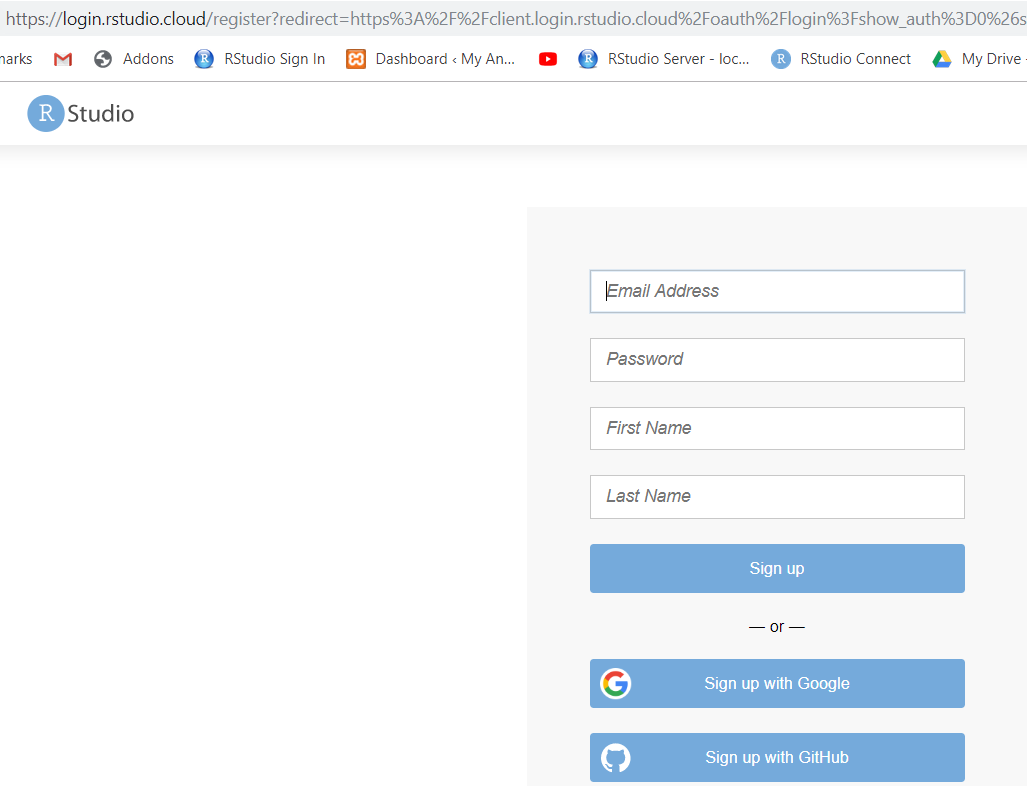
\includegraphics{cloud2.PNG}{]}

\hypertarget{point-and-click-r-gui}{%
\section{Point and click R GUI}\label{point-and-click-r-gui}}

There are a number of SPSS-like GUI for R. For example

\begin{itemize}
\tightlist
\item
  Bluesky statistics \url{https://www.blueskystatistics.com/}
\item
  JAMOVI - \url{https://www.jamovi.org/}
\end{itemize}

This is Bluesky statistics

{[}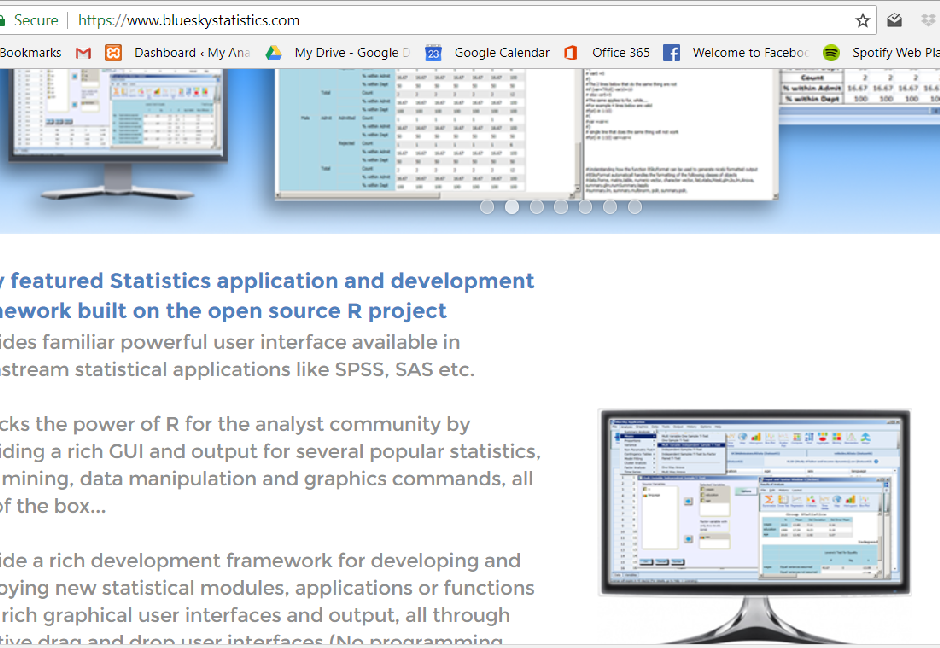
\includegraphics{bluesky.PNG}{]}

And this is JAMOVI

{[}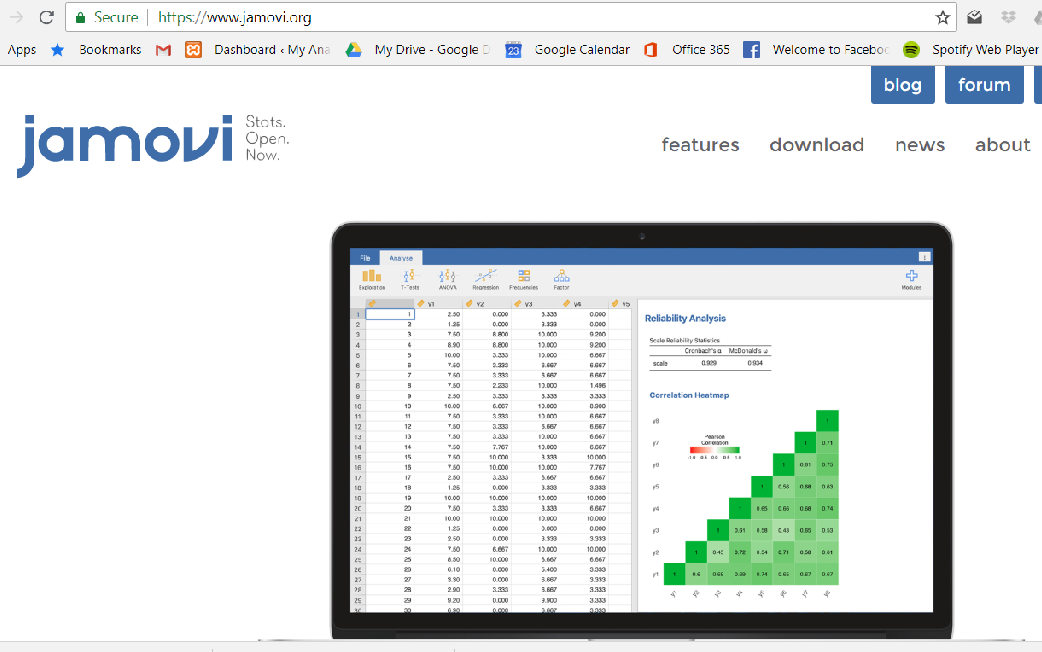
\includegraphics{jamovi.PNG}{]}

\hypertarget{rstudio-server}{%
\section{RStudio Server}\label{rstudio-server}}

You can run R and RStudio on the server. To do this you have to install RStudio Server. having RStudio Server enables you to do analysis on the server.

This will give a taste of working on BIG DATA. There are two versions of RStudio Server

\begin{itemize}
\tightlist
\item
  RStudio Server
\item
  RStudio Server Professional
\end{itemize}

For example, we have our RStudio Server Professional Edition (courtesy of RStudio) running on our server here \url{https://healthdata.usm.my/rstudio/auth-sign-in}

\hypertarget{installation}{%
\section{Installation}\label{installation}}

To install R on your machine, you have to have \textbf{Admin Right} to your machine. We recommend that you install

\begin{itemize}
\tightlist
\item
  R
\item
  RStudio
\end{itemize}

It is optional to install Latex editor for example MiKTeX and TeXLive for Windows and MacTex for Mac OS.

\hypertarget{installation-for-r}{%
\subsection{Installation for R}\label{installation-for-r}}

Though you can use R to run R codes. But we highly enciurage you to install both R and RStudio.

To install R, go to \href{https://cran.r-project.org/}{cran}. Then choose the correct R version for your machine OS. For example, for Windows OS the link is \url{https://cran.r-project.org/bin/windows/base/R-3.6.1-win.exe}. And for Mac OS, the download link is \url{https://cran.r-project.org/bin/macosx/R-3.6.1.pkg}. Similarly, if you are using Linux, follow the steps as listed before.

{[}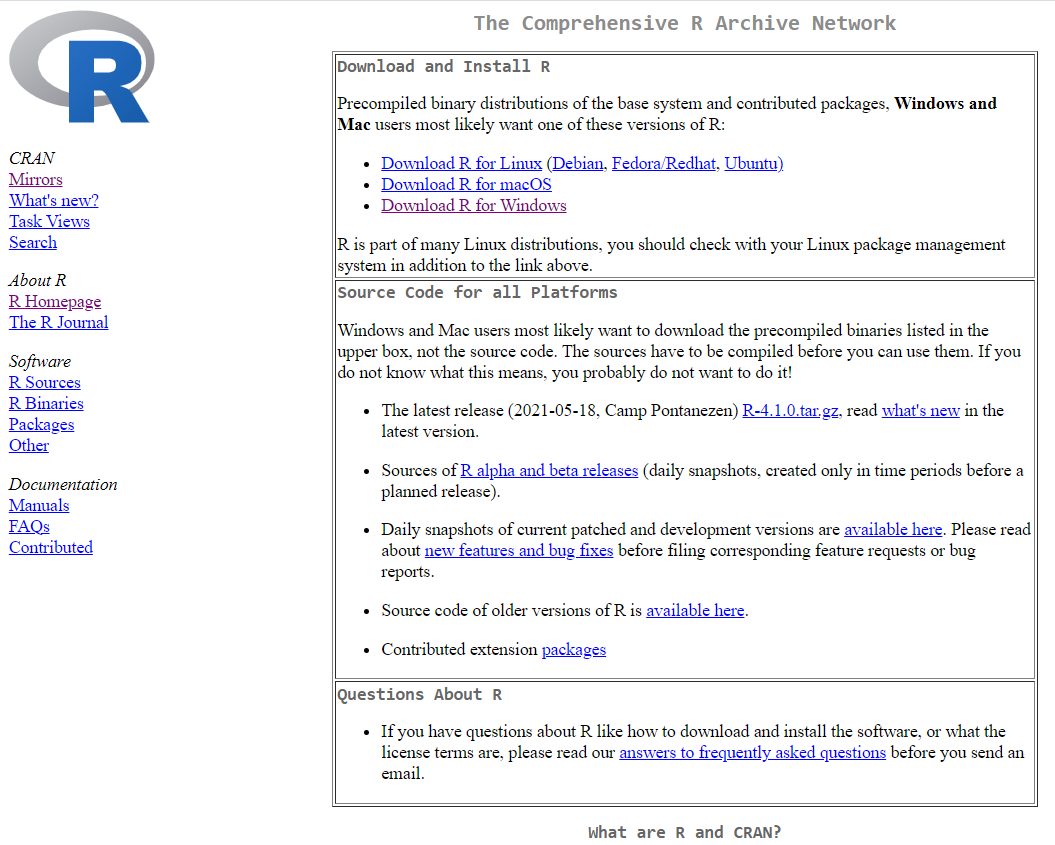
\includegraphics{cran.PNG}{]}

\hypertarget{installation-for-rstudio}{%
\subsection{Installation for RStudio}\label{installation-for-rstudio}}

You can install RStudio for your OS from here \url{https://www.rstudio.com/products/rstudio/download/\#download}. Choose the supported platforms. The size of download will be around 70-90 MB.

{[}
\includegraphics{rstudio2.PNG}{]}

\hypertarget{check-r-and-rstudio-on-your-machine}{%
\subsection{Check R and RStudio on your machine}\label{check-r-and-rstudio-on-your-machine}}

Now, we assume you have installed R and RStudio. Please, check

\begin{itemize}
\tightlist
\item
  Do you have R?
\item
  what version of R do you have?
\item
  Do you have RStudio?
\item
  what version of RStudio do you have?
\item
  Do you need to update R and RStudio?
\end{itemize}

\hypertarget{installation-of-miktex-texlive-and-mactex}{%
\subsection{Installation of MiKTeX, TeXLive and MacTex}\label{installation-of-miktex-texlive-and-mactex}}

It is necessary to install Latex editor if you want to convert the outputs to pdf. Especially, if you run your codes on RMarkdown. It is because RMarkdown can produce different types of documents.

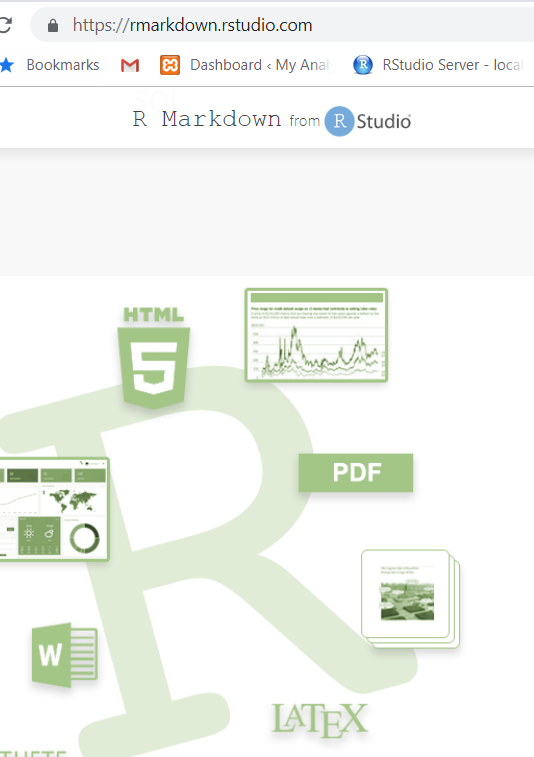
\includegraphics{rmarkdown.PNG}{]}

This is MiKTeX, for Window OS

\begin{figure}
\centering
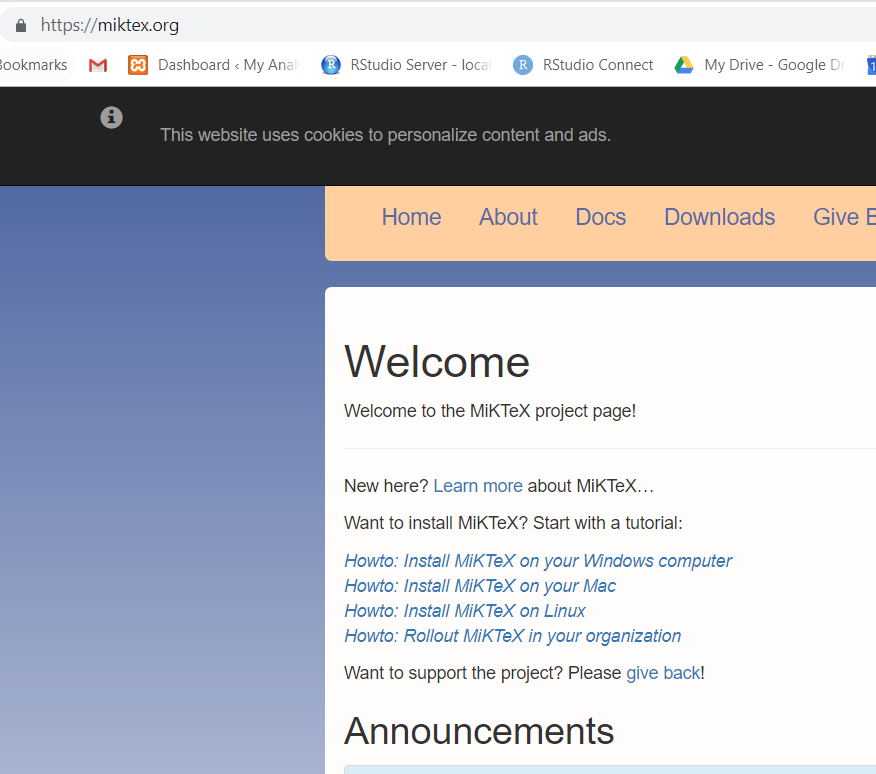
\includegraphics{miktex.PNG}
\caption{MikTeX webpage}
\end{figure}

And this is MacTeX, for Mac OS

\begin{figure}
\centering

\includegraphics{mactex.PNG}
\caption{MacTeX webpage}
\end{figure}

\hypertarget{start-your-rstudio}{%
\section{Start your RStudio}\label{start-your-rstudio}}

You can either login to RStudio Cloud OR start RStudio on your machine. remember, to login to RStudio Cloud, go to \url{https://rstudio.cloud}. Then you will be asked for your username and password.

Click this link \url{https://rstudio.cloud/spaces/44275/join?access_code=LPLoq5Q4kSdtBv1AN8kcHP\%2FHG0DiW1kGj4jVtG4k}

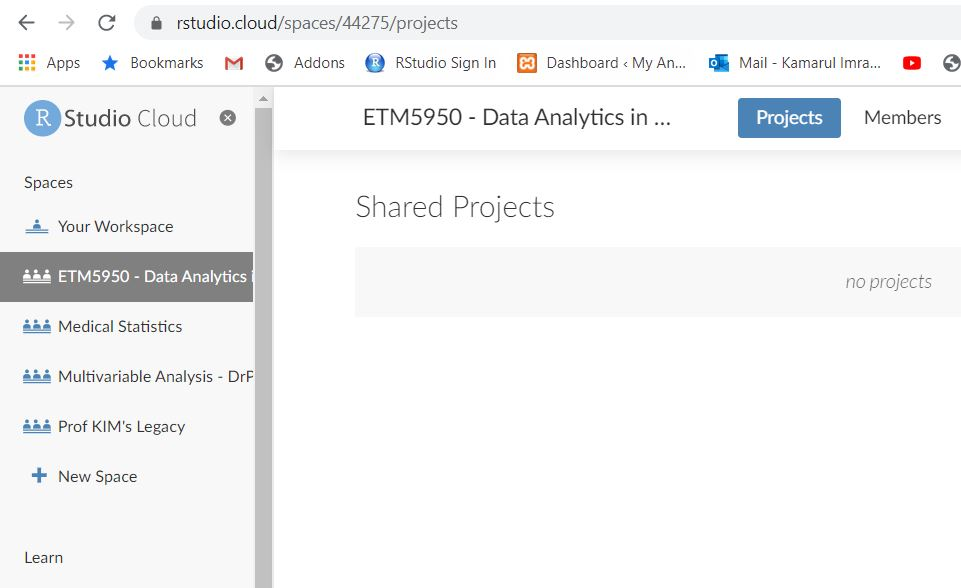
\includegraphics{etm5950.jpg}

To start R on your machine, find the Rstudio program in your start bar in your machine

\begin{figure}
\centering
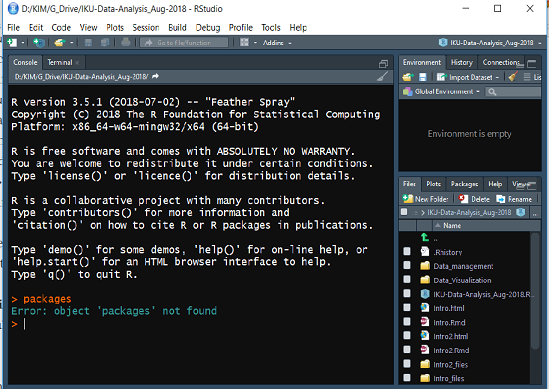
\includegraphics{rstudio.PNG}
\caption{Rstudio}
\end{figure}

What you see on RStudio now? You should see three panes if you start Rstudio for the first time or four panes if you have used RStudio before.

\begin{figure}
\centering
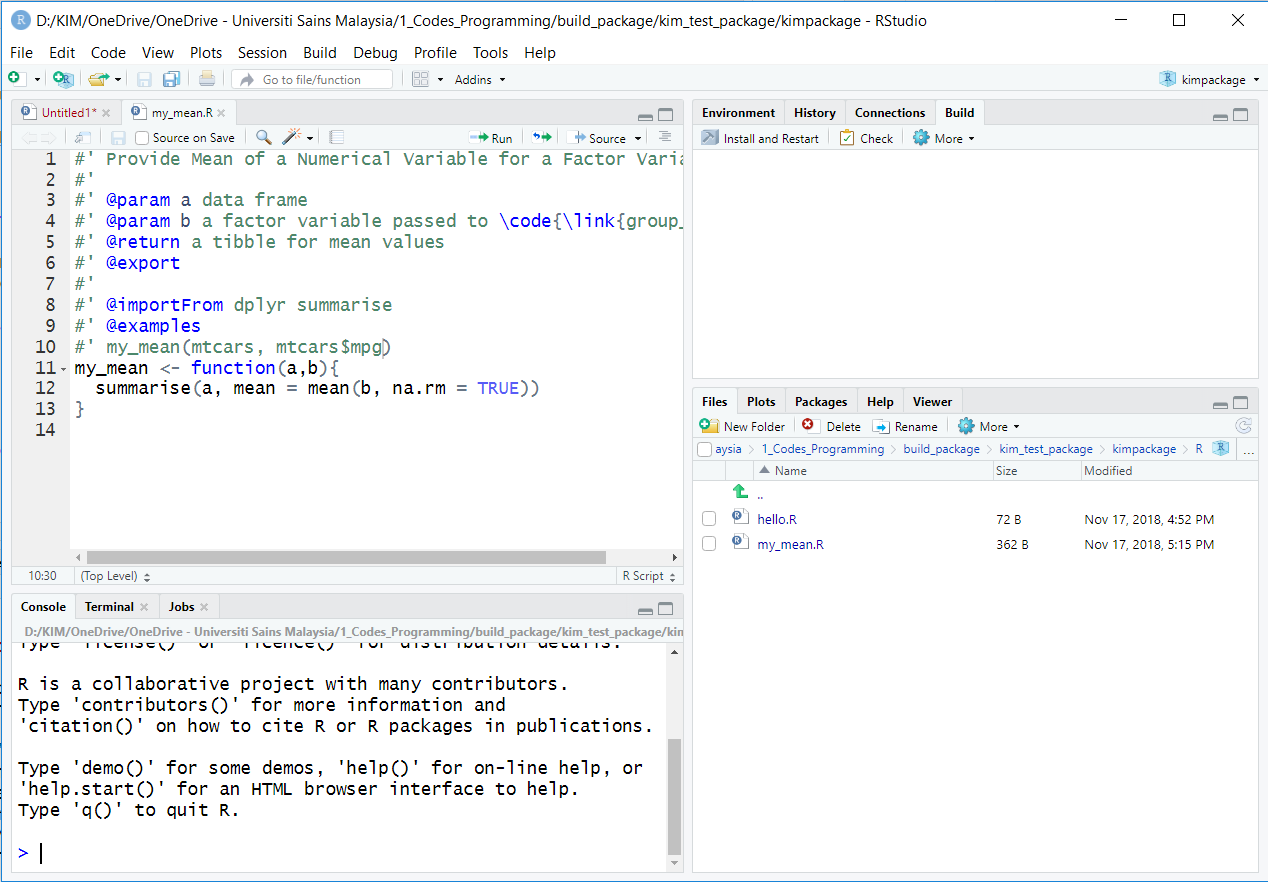
\includegraphics{rstudio_all.PNG}
\caption{RStudio Panes}
\end{figure}

\hypertarget{console-tab}{%
\subsection{Console tab}\label{console-tab}}

In Console tab, this is where we will see most of the results

\begin{figure}
\centering
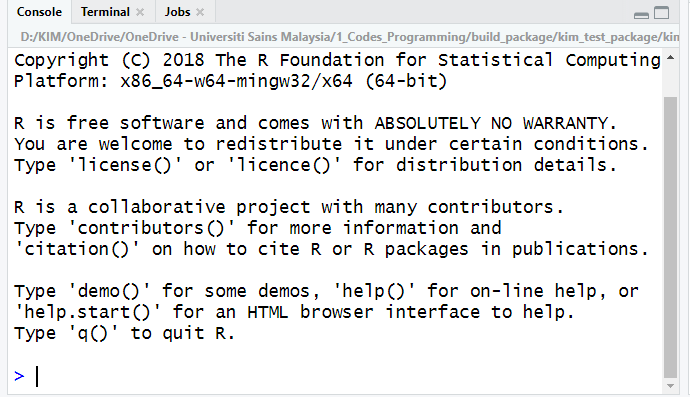
\includegraphics{console.PNG}
\caption{Console Pane}
\end{figure}

\hypertarget{files-plots-packages-help-and-viewer-pane}{%
\subsection{Files, Plots, Packages, Help and Viewer Pane}\label{files-plots-packages-help-and-viewer-pane}}

In this console, you will see

\begin{itemize}
\tightlist
\item
  List of objects
\item
  R files, datasets, tables, list etc
\end{itemize}

\begin{figure}
\centering
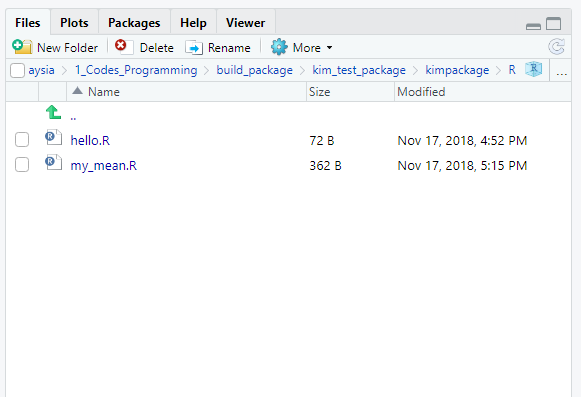
\includegraphics{files.PNG}
\caption{File, Plots and Viewer Pane}
\end{figure}

\hypertarget{environment-history-connection-and-build-pane}{%
\subsection{Environment, History, Connection and Build Pane}\label{environment-history-connection-and-build-pane}}

In the environment, history, connection and build pane, you will see this

\begin{figure}
\centering
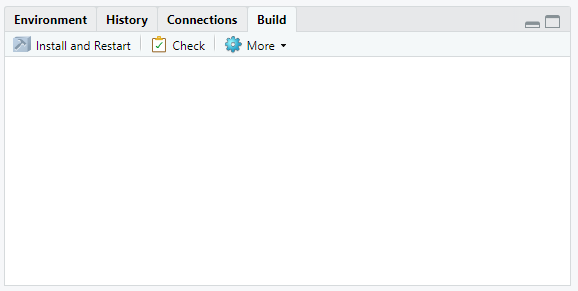
\includegraphics{envir.PNG}
\caption{Environment Pane}
\end{figure}

\hypertarget{source-pane}{%
\subsection{Source Pane}\label{source-pane}}

In the Source pane, you can create R files and write your R codes

\begin{figure}
\centering
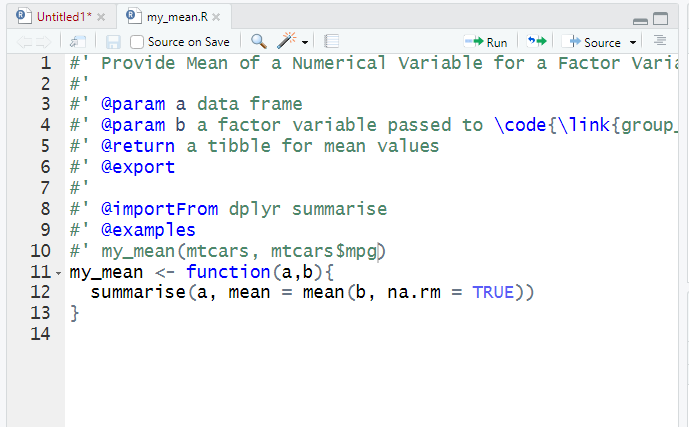
\includegraphics{source.PNG}
\caption{Source Pane}
\end{figure}

\hypertarget{open-a-new-r-script}{%
\section{Open a new R script}\label{open-a-new-r-script}}

To open a new R script

\begin{itemize}
\tightlist
\item
  File -\textgreater{} R Script
\item
  In Window OS, CTRL-SHIFT-N
\end{itemize}

\begin{figure}
\centering
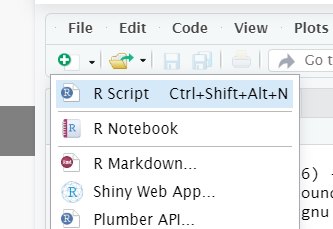
\includegraphics{Rscript.PNG}
\caption{New R Script}
\end{figure}

\hypertarget{our-first-r-script}{%
\subsection{Our first R script}\label{our-first-r-script}}

Let us write our first R script.

\begin{itemize}
\tightlist
\item
  In Line 1, type \texttt{2\ +\ 3}
\item
  click CTRL-ENTER or CMD-ENTER
\item
  see the outputs in the Console Pane
\end{itemize}

\begin{Shaded}
\begin{Highlighting}[]
\DecValTok{2} \SpecialCharTok{+} \DecValTok{3}
\end{Highlighting}
\end{Shaded}

\begin{verbatim}
## [1] 5
\end{verbatim}

After writing your R script, you can save it. This will allow to use or run the R script the next time you run RStudio.

To save R script

\begin{itemize}
\tightlist
\item
  File -\textgreater{}
\item
  Save As -\textgreater{}
\item
  Choose folder -\textgreater{}\\
\item
  Name the file
\end{itemize}

Now, types this to check the version of R

\begin{Shaded}
\begin{Highlighting}[]
\NormalTok{version[}\DecValTok{6}\SpecialCharTok{:}\DecValTok{7}\NormalTok{]}
\end{Highlighting}
\end{Shaded}

\begin{verbatim}
##       _  
## major 4  
## minor 1.0
\end{verbatim}

The current version for R is 4, 1.0

If you lower version, then you want to upgrade. To upgrade

\begin{itemize}
\tightlist
\item
  for Windows, you can use \textbf{installr} package
\item
  for Mac OS, you can use some functions
\end{itemize}

More info here \url{https://www.linkedin.com/pulse/3-methods-update-r-rstudio-windows-mac-woratana-ngarmtrakulchol/}

\hypertarget{function-argument-and-parameters}{%
\subsection{function, argument and parameters}\label{function-argument-and-parameters}}

R codes contain

\begin{itemize}
\tightlist
\item
  function
\item
  argument
\item
  parameters
\end{itemize}

\begin{verbatim}
f <- function(<arguments>) {
## Do something interesting
}
\end{verbatim}

For example, for the function \texttt{lm()} to estimate parameters for linear regression model

\begin{Shaded}
\begin{Highlighting}[]
\FunctionTok{args}\NormalTok{(lm)}
\end{Highlighting}
\end{Shaded}

\begin{verbatim}
## function (formula, data, subset, weights, na.action, method = "qr", 
##     model = TRUE, x = FALSE, y = FALSE, qr = TRUE, singular.ok = TRUE, 
##     contrasts = NULL, offset, ...) 
## NULL
\end{verbatim}

For example:

\begin{Shaded}
\begin{Highlighting}[]
\FunctionTok{lm}\NormalTok{(weight }\SpecialCharTok{\textasciitilde{}}\NormalTok{ Time, }\AttributeTok{data =}\NormalTok{ ChickWeight)}
\end{Highlighting}
\end{Shaded}

\begin{verbatim}
## 
## Call:
## lm(formula = weight ~ Time, data = ChickWeight)
## 
## Coefficients:
## (Intercept)         Time  
##      27.467        8.803
\end{verbatim}

Ref:

\begin{itemize}
\tightlist
\item
  \url{https://www.stat.auckland.ac.nz/~ihaka/downloads/Waikato-WRUG.pdf}
\item
  \url{https://www.stat.berkeley.edu/~statcur/Workshop2/Presentations/functions.pdf}
\end{itemize}

\hypertarget{need-more-help}{%
\subsection{Need more help?}\label{need-more-help}}

Then type the ? before the function

\begin{Shaded}
\begin{Highlighting}[]
\NormalTok{?lm}
\end{Highlighting}
\end{Shaded}

See what will be displayed in Help Pane

\begin{figure}
\centering
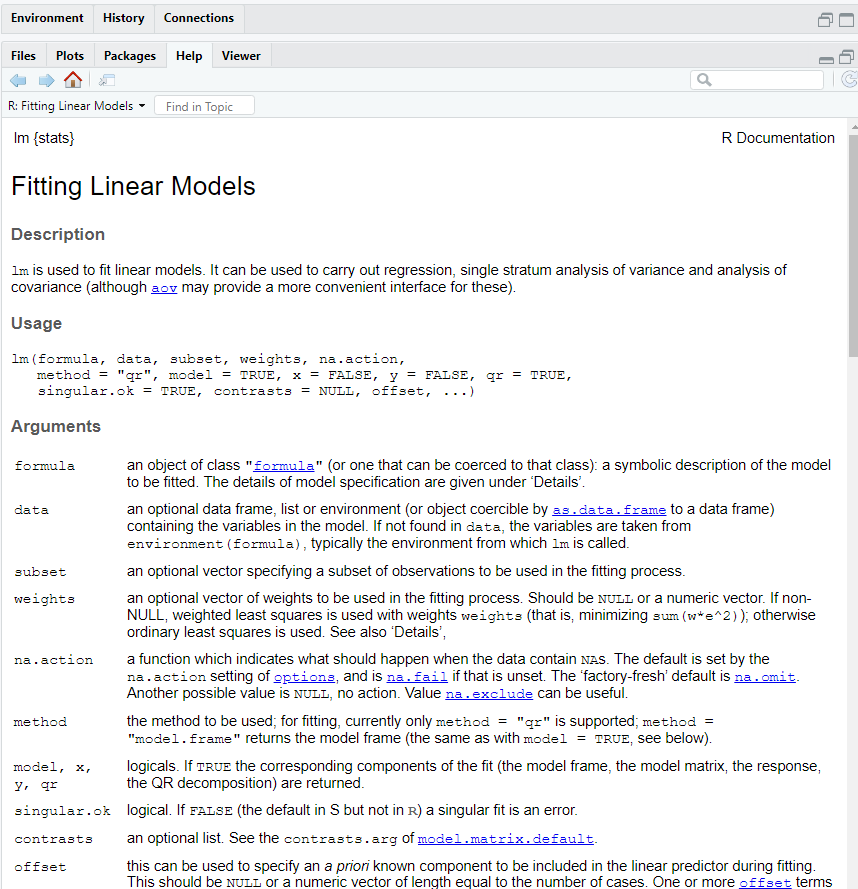
\includegraphics{lm.PNG}
\caption{Help Pane}
\end{figure}

\hypertarget{packages}{%
\section{Packages}\label{packages}}

\hypertarget{packages-on-cran}{%
\subsection{Packages on CRAN}\label{packages-on-cran}}

\url{https://cran.r-project.org/}

\begin{itemize}
\tightlist
\item
  Currently, the CRAN package repository features 12784 available packages
\item
  Cran Task Views
\end{itemize}

\begin{figure}
\centering
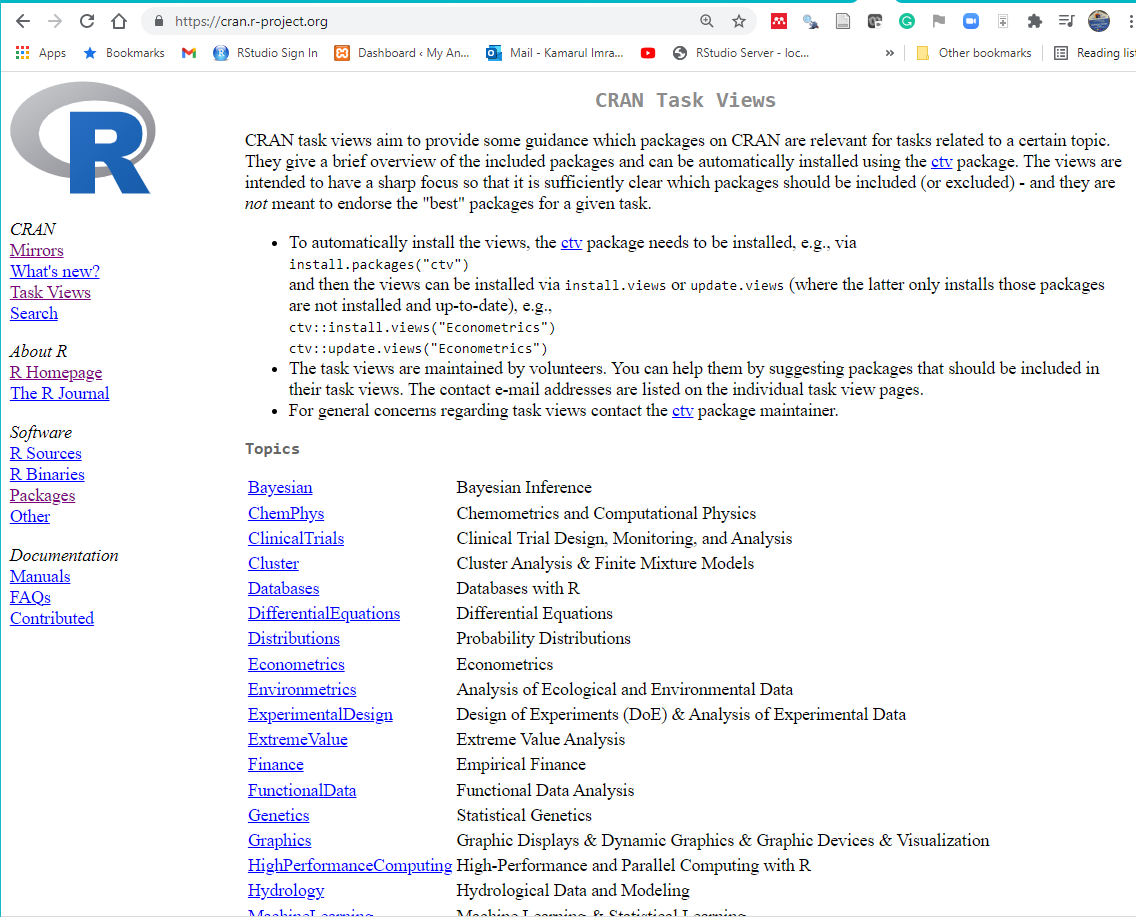
\includegraphics{packages.PNG}
\caption{Task Views}
\end{figure}

\hypertarget{check-if-the-package-you-need-is-available-in-your-r-library}{%
\subsection{Check if the package you need is available in your R library}\label{check-if-the-package-you-need-is-available-in-your-r-library}}

Type this inside your console

\begin{Shaded}
\begin{Highlighting}[]
\FunctionTok{library}\NormalTok{(ggplot2)}
\end{Highlighting}
\end{Shaded}

You should not receive any error message. If you have not installed the package, you will receive and error message. And it tells you that the package is not available in your R. the package is stored in the R folder in your My Document or HOME directory

\begin{Shaded}
\begin{Highlighting}[]
\FunctionTok{.libPaths}\NormalTok{()}
\end{Highlighting}
\end{Shaded}

\begin{verbatim}
## [1] "C:/Users/drkim/OneDrive/Documents/R/win-library/4.1"
## [2] "C:/Program Files/R/R-4.1.0/library"
\end{verbatim}

\hypertarget{install-an-r-package}{%
\subsection{Install an R package}\label{install-an-r-package}}

To install an R package, you can type below (without the \# tag)

\begin{Shaded}
\begin{Highlighting}[]
\CommentTok{\# install.packages(foreign, dependencies = TRUE)}
\end{Highlighting}
\end{Shaded}

You need to have internet access. You can install from a zip file (from your machine or USB), from github and other repo

\hypertarget{directory}{%
\section{Directory}\label{directory}}

This is important. Not knowing your working directory will make you lost (you do not know where your R codes, R outputs, datasets etc)

You must know where your folder is located. The folder can contain many sub folders. The folder should contain dataset (if you want to analyze your data). It will later store the objects created during R session

\begin{Shaded}
\begin{Highlighting}[]
\FunctionTok{getwd}\NormalTok{()}
\end{Highlighting}
\end{Shaded}

\begin{verbatim}
## [1] "C:/Users/drkim/OneDrive - Universiti Sains Malaysia/multivar_data_analysis"
\end{verbatim}

You have to know to write file path. It is written differently for Window OS and other OS

\hypertarget{starting-your-r-job}{%
\subsection{Starting your R job}\label{starting-your-r-job}}

There are 2 ways to start your job:

\begin{itemize}
\tightlist
\item
  create a new project (recommended)
\item
  setting your working directory using \texttt{setwd()} (not recommended)
\end{itemize}

\hypertarget{create-new-project}{%
\subsection{Create new project}\label{create-new-project}}

Always create a new project (This is the recommended way). This can be by

\begin{itemize}
\tightlist
\item
  Go to \texttt{File\ -\textgreater{}\ New\ Project}
\end{itemize}

{[}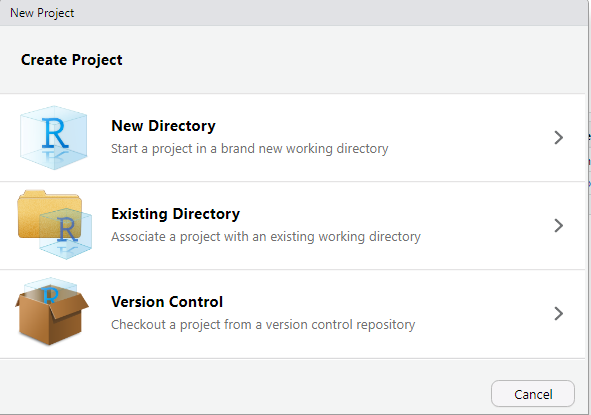
\includegraphics{new_proj.PNG}{]}

When you see project type, click New Project

\begin{figure}
\centering
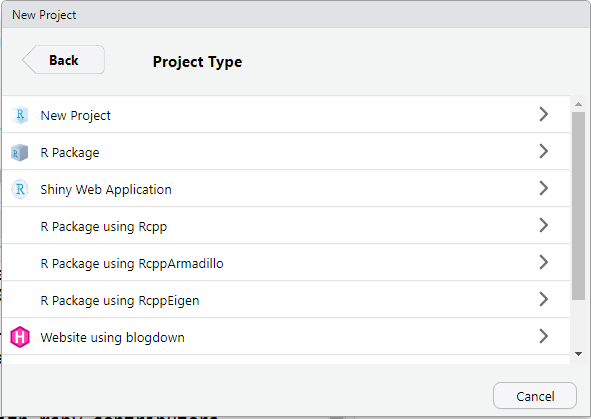
\includegraphics{new_proj2.PNG}
\caption{Project Type}
\end{figure}

\hypertarget{where-is-my-data}{%
\subsection{Where is my data?}\label{where-is-my-data}}

Datasets for analysis in R and usually in data frame format. You can see the datasets in the environment pane. Your data is read from the original dataset to a memory. SO you must know the size of your computer RAM. How much your RAM for your machine? The bigger the RAM, thelarger R can read and store your data.

The data that is read (in memory) will dissaper once you close RStudio. But the original stays in its location. This will not change your original data (so be happy!)

\begin{figure}
\centering
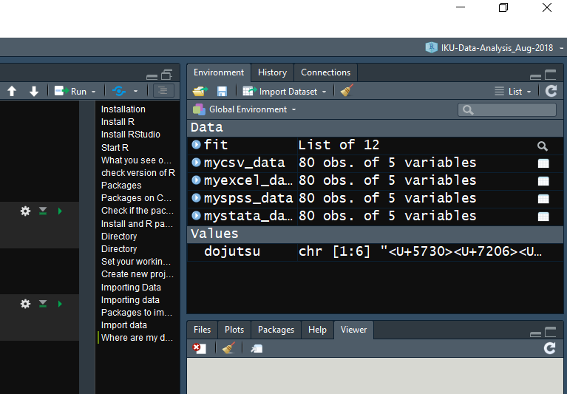
\includegraphics{mydata.PNG}
\caption{My Data}
\end{figure}

\hypertarget{upload-data-to-rstudio-cloud}{%
\section{Upload data to RStudio Cloud}\label{upload-data-to-rstudio-cloud}}

You have to upload data to RStudio Cloud Or link data to dropbox folder

\begin{figure}
\centering
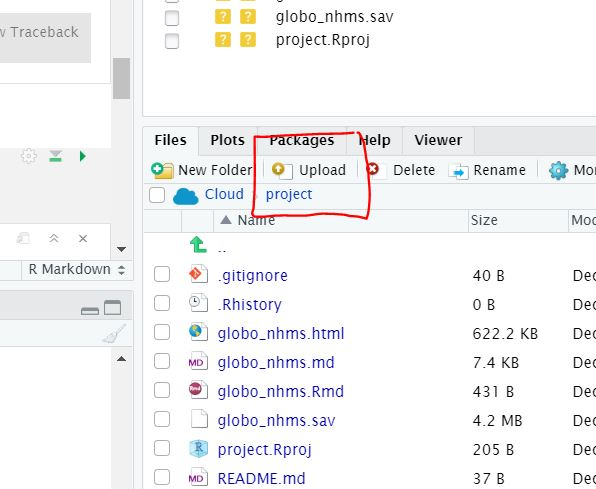
\includegraphics{upload_data.jpg}
\caption{Upload Data in RStudio Cloud}
\end{figure}

\hypertarget{more-resources-on-rstudio-cloud}{%
\section{More resources on RStudio Cloud}\label{more-resources-on-rstudio-cloud}}

You can learn more about RStudio Cloud here

\begin{itemize}
\item
  on YouTube : RStudio Cloud for educationn \url{https://www.youtube.com/watch?v=PviVimazpz8}
\item
  YouTube: Working with R in Cloud \url{https://www.youtube.com/watch?v=SFpzr21Pavg}
\end{itemize}

\hypertarget{need-help}{%
\section{Need help?}\label{need-help}}

If you need help you can

\begin{itemize}
\tightlist
\item
  Type a question mark infront of a function
\end{itemize}

\begin{Shaded}
\begin{Highlighting}[]
\NormalTok{?plot}
\end{Highlighting}
\end{Shaded}

Other options are these:

\begin{itemize}
\tightlist
\item
  register and join RStudio Community here \url{https://community.rstudio.com/}
\item
  Ask questions on Stack Overflow \url{https://stackoverflow.com/}
\item
  Search for mailing list and subscribe to it
\item
  Books on R \url{https://bookdown.org/}
\end{itemize}

\hypertarget{bookdown}{%
\section{Bookdown}\label{bookdown}}

This webpage contains many useful books that use R codes \url{https://bookdown.org/}

\begin{figure}
\centering

\includegraphics{bookdown.PNG}
\caption{Bookdown}
\end{figure}

\hypertarget{data-visualization}{%
\chapter{Data Visualization}\label{data-visualization}}

\hypertarget{introduction-to-visualization}{%
\section{Introduction to visualization}\label{introduction-to-visualization}}

Data visualization is viewed by many disciplines as a modern equivalent of visual communication. It involves the creation and study of the visual representation of data. Data visualization requires ``information that has been abstracted in some schematic form, including attributes or variables for the units of information''. You can read more about data visualization here \url{https://en.m.wikipedia.org/wiki/Data_visualization} and here \url{https://en.m.wikipedia.org/wiki/Michael_Friendly}

\hypertarget{history-of-data-visualization}{%
\subsection{History of data visualization}\label{history-of-data-visualization}}

In his 1983 book which carried the title \emph{The Visual Display of Quantitative Information}, the author Edward Tufte defines \textbf{graphical displays} and principles for effective graphical display. The book mentioned that ``Excellence in statistical graphics consists of complex ideas communicated with clarity, precision and efficiency.''

\hypertarget{processes-and-objectives-of-visualization}{%
\subsection{Processes and Objectives of visualization}\label{processes-and-objectives-of-visualization}}

Visualization is the process of representing data graphically and interacting with these representations. The objective is to gain insight into the data. Some of the processes are outlined here \url{http://researcher.watson.ibm.com/researcher/view_group.php?id=143}

\hypertarget{what-makes-good-graphics}{%
\section{What makes good graphics}\label{what-makes-good-graphics}}

You may require these to make good graphics:

\begin{enumerate}
\def\labelenumi{\arabic{enumi}.}
\tightlist
\item
  Data
\item
  Substance rather than about methodology, graphic design, the technology of graphic production or something else
\item
  No distortion to what the data has to say
\item
  Presence of many numbers in a small space
\item
  Coherence for large data sets
\item
  Encourage the eye to compare different pieces of data
\item
  Reveal the data at several levels of detail, from a broad overview to the fine structure
\item
  Serve a reasonably clear purpose: description, exploration, tabulation or decoration
\item
  Be closely integrated with the statistical and verbal descriptions of a data set.
\end{enumerate}

\hypertarget{graphics-packages-in-r}{%
\section{Graphics packages in R}\label{graphics-packages-in-r}}

There are many \textbf{graphics packages} in R. Some packages are aimed to perform general tasks related with graphs. Some provide specific graphics for certain analyses. The popular general graphics packages in R are:

\begin{enumerate}
\def\labelenumi{\arabic{enumi}.}
\tightlist
\item
  \textbf{graphics} : a base R package
\item
  \textbf{ggplot2} : a user-contributed package by Hadley Wickham
\item
  \textbf{lattice} : a user-contributed package
\end{enumerate}

Except for \textbf{graphics} package (a a base R package), other packages need to downloaded and installed into your R library. Examples of other more specific packages - to run graphics for certain analyses - are:

\begin{enumerate}
\def\labelenumi{\arabic{enumi}.}
\tightlist
\item
  \textbf{survminer::ggsurvlot}
\item
  \textbf{sjPlot}
\end{enumerate}

For this course, we will focus on using the \textbf{ggplot2} package.

\hypertarget{introduction-to-ggplot2-package}{%
\section{\texorpdfstring{Introduction to \textbf{ggplot2} package}{Introduction to ggplot2 package}}\label{introduction-to-ggplot2-package}}

The \textbf{ggplot2} package is an elegant, easy and versatile general graphics package in R. It implements the \textbf{grammar of graphics} concept. The advantage of this concept is that, it fasten the process of learning graphics. It also facilitates the process of creating complex graphics

To work with \textbf{ggplot2}, remember

\begin{itemize}
\tightlist
\item
  start with: \texttt{ggplot()}
\item
  which data: \texttt{data\ =\ X}
\item
  which variables: \texttt{aes(x\ =\ ,\ y\ =\ )}
\item
  which graph: \texttt{geom\_histogram()}, \texttt{geom\_points()}
\end{itemize}

The official website for ggplot2 is here \url{http://ggplot2.org/}.

\emph{ggplot2 is a plotting system for R, based on the grammar of graphics, which tries to take the good parts of base and lattice graphics and none of the bad parts. It takes care of many of the fiddly details that make plotting a hassle (like drawing legends) as well as providing a powerful model of graphics that makes it easy to produce complex multi-layered graphics.}

\hypertarget{preparation}{%
\section{Preparation}\label{preparation}}

\hypertarget{set-a-new-project-or-set-the-working-directory}{%
\subsection{Set a new project or set the working directory}\label{set-a-new-project-or-set-the-working-directory}}

It is always recommended that to start working on data analysis in RStudio, you create first a new project.

Go to File, then click New Project.

You can create a new R project based on existing directory. This method is useful because an RStudio project keep your data, your analysis, and outputs in a clean dedicated folder or sets of folders.If you do not want to create a new project, then make sure you are inside the correct directory (the working directory). The working directory is a folder where you store.

Type \texttt{getwd()} in your Console to display your working directory. Inside your working directory, you should see and keep

\begin{enumerate}
\def\labelenumi{\arabic{enumi}.}
\tightlist
\item
  dataset or datasets
\item
  outputs - plots
\item
  codes (R scripts \texttt{.R}, R markdown files \texttt{.Rmd})
\end{enumerate}

\hypertarget{questions-to-ask-before-making-graphs}{%
\subsection{Questions to ask before making graphs}\label{questions-to-ask-before-making-graphs}}

You must ask yourselves these:

\begin{enumerate}
\def\labelenumi{\arabic{enumi}.}
\tightlist
\item
  Which variable or variables do I want to plot?
\item
  What is (or are) the type of that variable?
\end{enumerate}

\begin{itemize}
\tightlist
\item
  Are they factor (categorical) variables ?
\item
  Are they numerical variables?
\end{itemize}

\begin{enumerate}
\def\labelenumi{\arabic{enumi}.}
\setcounter{enumi}{2}
\tightlist
\item
  Am I going to plot
\end{enumerate}

\begin{itemize}
\tightlist
\item
  a single variable?
\item
  two variables together?
\item
  three variables together?
\end{itemize}

\hypertarget{read-data}{%
\subsection{Read data}\label{read-data}}

The common data formats include

\begin{enumerate}
\def\labelenumi{\arabic{enumi}.}
\tightlist
\item
  comma separated files (\texttt{.csv})
\item
  MS Excel file (\texttt{.xlsx})
\item
  SPSS file (\texttt{.sav})
\item
  Stata file (\texttt{.dta})
\item
  SAS file
\end{enumerate}

Packages that read these data include \textbf{haven} package. Below are the functions to read SAS, SPSS and Stata file.

\begin{enumerate}
\def\labelenumi{\arabic{enumi}.}
\tightlist
\item
  SAS: \texttt{read\_sas()} reads .sas7bdat + .sas7bcat files and read\_xpt() reads SAS transport files (version 5 and version 8). write\_sas() writes .sas7bdat files.
\item
  SPSS: \texttt{read\_sav()} reads .sav files and read\_por() reads the older .por files. write\_sav() writes .sav files.
\item
  Stata: \texttt{read\_dta()} reads .dta files (up to version 15). write\_dta() writes .dta files (versions 8-15).
\end{enumerate}

Data from databases are less common but are getting more important and more common. R can also read these data. Some examples of databases format are:

\begin{enumerate}
\def\labelenumi{\arabic{enumi}.}
\tightlist
\item
  MySQL
\item
  SQLite
\item
  Postgresql
\item
  Mariadb
\end{enumerate}

\hypertarget{load-the-library}{%
\subsection{Load the library}\label{load-the-library}}

The \textbf{ggplot2} package is one of the core member of \textbf{tidyverse} package (\url{https://www.tidyverse.org/}). So, if we load the \textbf{tidyverse} package, we will access to other packages under \textbf{tidyverse} which include \textbf{dplyr}, \textbf{readr}, \textbf{ggplot2}.

Loading a package will give you access to

\begin{enumerate}
\def\labelenumi{\arabic{enumi}.}
\tightlist
\item
  help pages
\item
  functions
\item
  datasets
\end{enumerate}

\begin{Shaded}
\begin{Highlighting}[]
\FunctionTok{library}\NormalTok{(tidyverse)}
\end{Highlighting}
\end{Shaded}

If you run the code and you see \emph{there is no package called tidyverse} then you need to install the \textbf{tidyverse} package. To install the package, type \texttt{install.package("tidyverse")} in the Console. Once the installation is complete, type \texttt{library(tidyverse)} to load the package.

\hypertarget{open-dataset}{%
\subsection{Open dataset}\label{open-dataset}}

For now, we will use the built-in dataset in the \textbf{gapminder} package. You can read more about \emph{gapminder} from \url{https://www.gapminder.org/}. The gapminder website contains many useful datasets and show wonderful graphics. It is made popular by Dr Hans Rosling.

To load the package, type

\begin{Shaded}
\begin{Highlighting}[]
\FunctionTok{library}\NormalTok{(gapminder)}
\end{Highlighting}
\end{Shaded}

call the data \emph{gapminder} into R and browse the first 6 observations of the \emph{gapminder} data

\begin{Shaded}
\begin{Highlighting}[]
\NormalTok{gapminder }\OtherTok{\textless{}{-}}\NormalTok{ gapminder}
\FunctionTok{head}\NormalTok{(gapminder)}
\end{Highlighting}
\end{Shaded}

\begin{verbatim}
## # A tibble: 6 x 6
##   country     continent  year lifeExp      pop gdpPercap
##   <fct>       <fct>     <int>   <dbl>    <int>     <dbl>
## 1 Afghanistan Asia       1952    28.8  8425333      779.
## 2 Afghanistan Asia       1957    30.3  9240934      821.
## 3 Afghanistan Asia       1962    32.0 10267083      853.
## 4 Afghanistan Asia       1967    34.0 11537966      836.
## 5 Afghanistan Asia       1972    36.1 13079460      740.
## 6 Afghanistan Asia       1977    38.4 14880372      786.
\end{verbatim}

We can list the variables and look at the type of the variables in the dataset

\begin{Shaded}
\begin{Highlighting}[]
\FunctionTok{glimpse}\NormalTok{(gapminder)}
\end{Highlighting}
\end{Shaded}

\begin{verbatim}
## Rows: 1,704
## Columns: 6
## $ country   <fct> "Afghanistan", "Afghanistan", "Afghanistan", "Afghanistan", ~
## $ continent <fct> Asia, Asia, Asia, Asia, Asia, Asia, Asia, Asia, Asia, Asia, ~
## $ year      <int> 1952, 1957, 1962, 1967, 1972, 1977, 1982, 1987, 1992, 1997, ~
## $ lifeExp   <dbl> 28.801, 30.332, 31.997, 34.020, 36.088, 38.438, 39.854, 40.8~
## $ pop       <int> 8425333, 9240934, 10267083, 11537966, 13079460, 14880372, 12~
## $ gdpPercap <dbl> 779.4453, 820.8530, 853.1007, 836.1971, 739.9811, 786.1134, ~
\end{verbatim}

The \emph{gapminder} data have

\begin{enumerate}
\def\labelenumi{\arabic{enumi}.}
\tightlist
\item
  6 variables
\item
  1704 observations
\item
  There are 2 factor variables, 2 integer variables and 2 numeric variables
\end{enumerate}

We can examine the basic statistics of the datasets by using \texttt{summary()}. This function will list

\begin{enumerate}
\def\labelenumi{\arabic{enumi}.}
\tightlist
\item
  the frequencies
\item
  some descriptive statistics: min, 1st quartile, median, mean, 3rd quartile and max
\end{enumerate}

\begin{Shaded}
\begin{Highlighting}[]
\FunctionTok{summary}\NormalTok{(gapminder)}
\end{Highlighting}
\end{Shaded}

\begin{verbatim}
##         country        continent        year         lifeExp     
##  Afghanistan:  12   Africa  :624   Min.   :1952   Min.   :23.60  
##  Albania    :  12   Americas:300   1st Qu.:1966   1st Qu.:48.20  
##  Algeria    :  12   Asia    :396   Median :1980   Median :60.71  
##  Angola     :  12   Europe  :360   Mean   :1980   Mean   :59.47  
##  Argentina  :  12   Oceania : 24   3rd Qu.:1993   3rd Qu.:70.85  
##  Australia  :  12                  Max.   :2007   Max.   :82.60  
##  (Other)    :1632                                                
##       pop              gdpPercap       
##  Min.   :6.001e+04   Min.   :   241.2  
##  1st Qu.:2.794e+06   1st Qu.:  1202.1  
##  Median :7.024e+06   Median :  3531.8  
##  Mean   :2.960e+07   Mean   :  7215.3  
##  3rd Qu.:1.959e+07   3rd Qu.:  9325.5  
##  Max.   :1.319e+09   Max.   :113523.1  
## 
\end{verbatim}

To know more about the package, we can use the \(?\) mark

\begin{Shaded}
\begin{Highlighting}[]
\NormalTok{?gapminder}
\end{Highlighting}
\end{Shaded}

\hypertarget{basic-plot}{%
\section{Basic plot}\label{basic-plot}}

We can start create a basic plot by setting these parameters

\begin{itemize}
\tightlist
\item
  data = gapminder
\item
  variables = year, lifeExp
\item
  graph = scatterplot
\end{itemize}

In \textbf{ggplot2} which is a package under \textbf{tidyverse} package, you can use the \(+\) sign to connect the function. And in R, your codes can span multiple lines. This will increase the visibility of the codes.

\begin{Shaded}
\begin{Highlighting}[]
\FunctionTok{ggplot}\NormalTok{(}\AttributeTok{data =}\NormalTok{ gapminder) }\SpecialCharTok{+}
  \FunctionTok{geom\_point}\NormalTok{(}\AttributeTok{mapping =} \FunctionTok{aes}\NormalTok{(}\AttributeTok{x =}\NormalTok{ year, }\AttributeTok{y =}\NormalTok{ lifeExp))}
\end{Highlighting}
\end{Shaded}

\begin{center}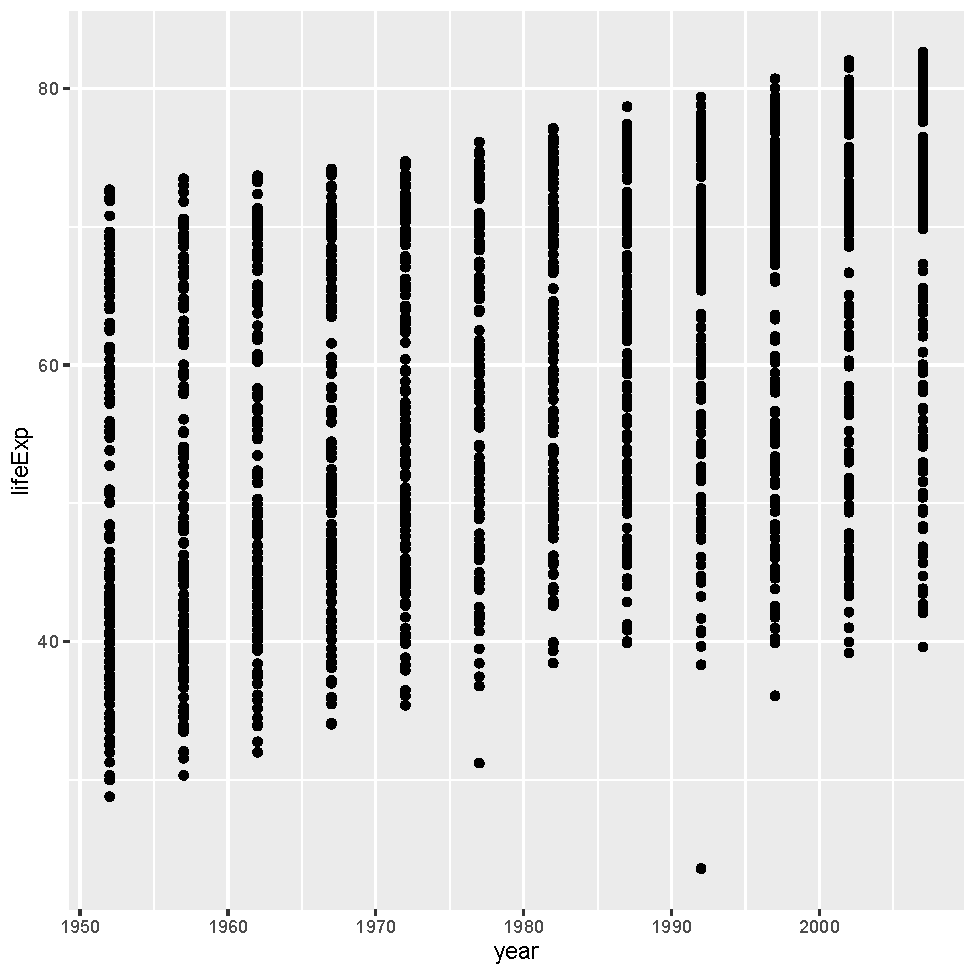
\includegraphics[width=0.7\linewidth,keepaspectratio]{Multivariable_Data_Analysis_files/figure-latex/unnamed-chunk-17-1} \end{center}

Now, you can see that the plot shows:

\begin{enumerate}
\def\labelenumi{\arabic{enumi}.}
\tightlist
\item
  the relationship between year and life expectancy.
\item
  as variable year advances, the life expectancy increases.
\end{enumerate}

the \texttt{ggplot()} tells R to plot what variables from what data. And \texttt{geom\_point()} tells R to make a scatter plot.

\hypertarget{adding-another-variable}{%
\section{Adding another variable}\label{adding-another-variable}}

You realize that we plotted 2 variables based on \texttt{aes()}. We can add the third variable to make a more complicated plot. For example:

\begin{enumerate}
\def\labelenumi{\arabic{enumi}.}
\tightlist
\item
  data = gapminder
\item
  variables = year, life expectancy, continent
\end{enumerate}

For this, the objective to create plot might be to see the relationship between year and life expectancy based on continent.

\begin{Shaded}
\begin{Highlighting}[]
\FunctionTok{ggplot}\NormalTok{(}\AttributeTok{data =}\NormalTok{ gapminder) }\SpecialCharTok{+}
  \FunctionTok{geom\_point}\NormalTok{(}\AttributeTok{mapping =} \FunctionTok{aes}\NormalTok{(}\AttributeTok{x =}\NormalTok{ year, }\AttributeTok{y =}\NormalTok{ lifeExp, }\AttributeTok{colour =}\NormalTok{ continent))}
\end{Highlighting}
\end{Shaded}

\begin{center}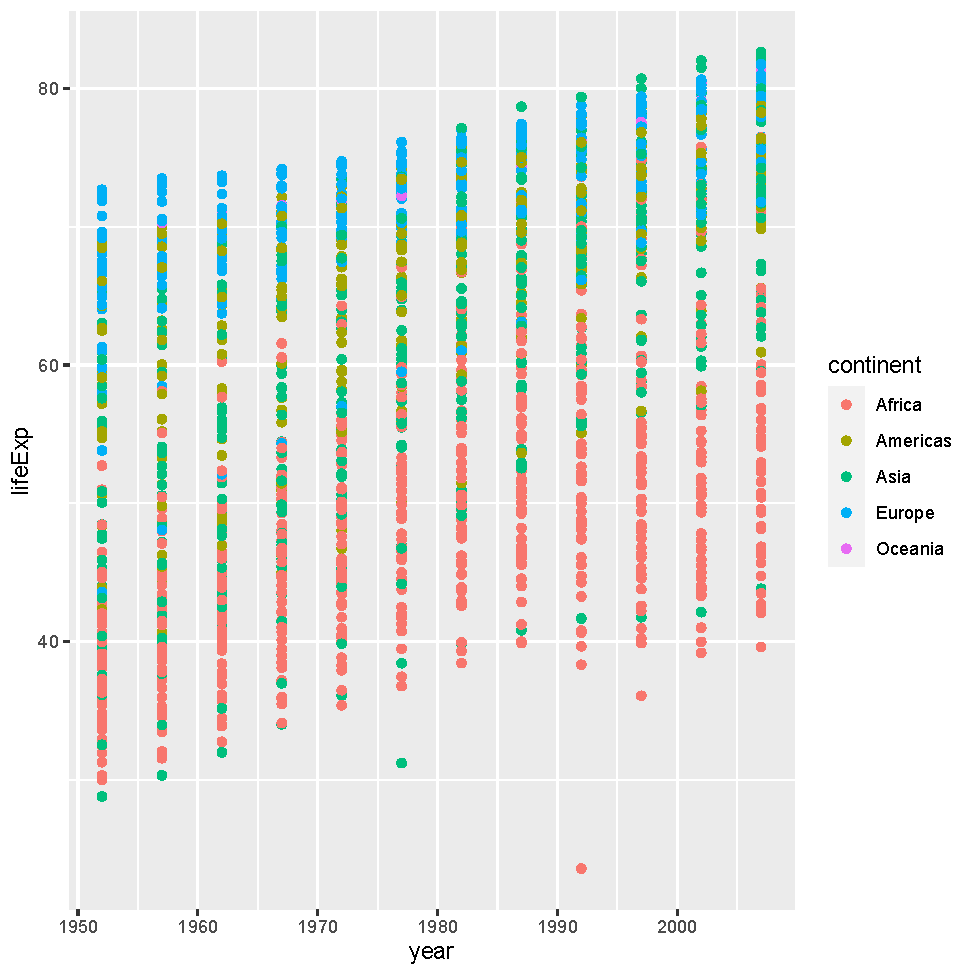
\includegraphics[width=0.7\linewidth,keepaspectratio]{Multivariable_Data_Analysis_files/figure-latex/unnamed-chunk-18-1} \end{center}

What can you see from the scatterplot? You may notice that

\begin{enumerate}
\def\labelenumi{\arabic{enumi}.}
\tightlist
\item
  Europe countries have high life expectancy
\item
  Africa countries have lower life expectancy
\item
  One Asia country looks like an outlier (very low life expectancy)
\item
  One Africa country looks like an outlier (very low life expectancy)
\end{enumerate}

Now, we will replace the 3rd variable with GDP (variable gdpPercap) and make the plot correlates with the size of GDP.

\begin{Shaded}
\begin{Highlighting}[]
\FunctionTok{ggplot}\NormalTok{(}\AttributeTok{data =}\NormalTok{ gapminder) }\SpecialCharTok{+}
  \FunctionTok{geom\_point}\NormalTok{(}\AttributeTok{mapping =} \FunctionTok{aes}\NormalTok{(}\AttributeTok{x =}\NormalTok{ year, }\AttributeTok{y =}\NormalTok{ lifeExp, }\AttributeTok{size =}\NormalTok{ gdpPercap))}
\end{Highlighting}
\end{Shaded}

\begin{center}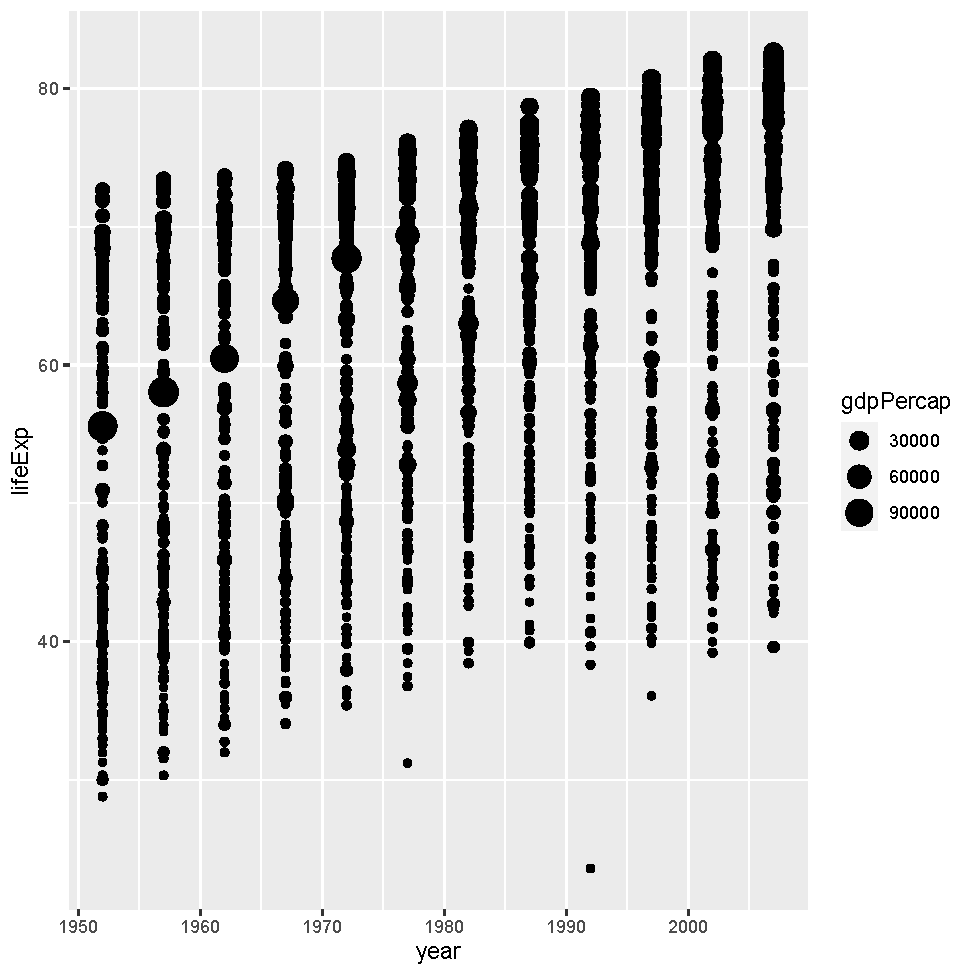
\includegraphics[width=0.7\linewidth,keepaspectratio]{Multivariable_Data_Analysis_files/figure-latex/unnamed-chunk-19-1} \end{center}

\emph{ggplot2} will automatically assign a unique level of the aesthetic (here a unique color) to each unique value of the variable, a process known as scaling. \emph{ggplot2} will also add a legend that explains which levels correspond to which values. The plot suggets that higher GDP countries have longer life expectancy.

Instead of using colour, we can use shape especially in instances where there is no facility to print out colour plots.

\begin{Shaded}
\begin{Highlighting}[]
\FunctionTok{ggplot}\NormalTok{(}\AttributeTok{data =}\NormalTok{ gapminder) }\SpecialCharTok{+}
  \FunctionTok{geom\_point}\NormalTok{(}\AttributeTok{mapping =} \FunctionTok{aes}\NormalTok{(}\AttributeTok{x =}\NormalTok{ year, }\AttributeTok{y =}\NormalTok{ lifeExp, }\AttributeTok{shape =}\NormalTok{ continent))}
\end{Highlighting}
\end{Shaded}

\begin{center}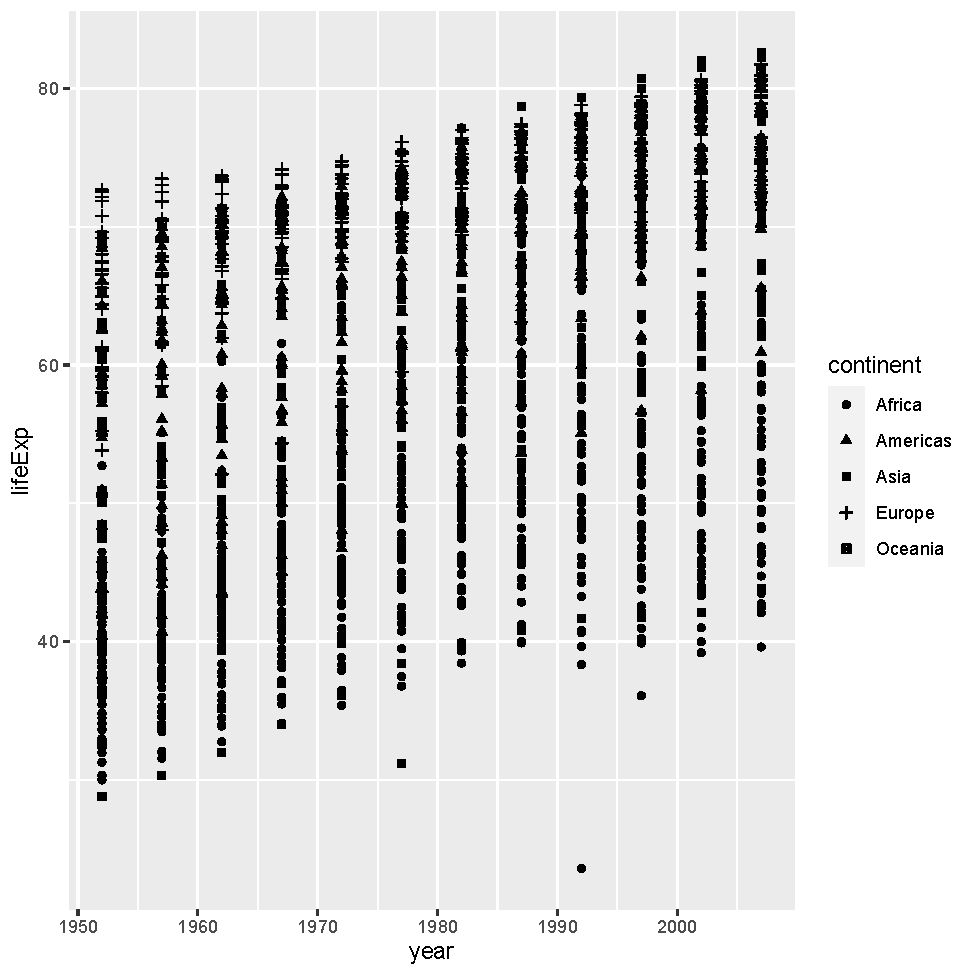
\includegraphics[width=0.7\linewidth,keepaspectratio]{Multivariable_Data_Analysis_files/figure-latex/unnamed-chunk-20-1} \end{center}

But, see what will happen if you set the colour and shape like below but outside the aes parentheses. For example, let set the parameter colour to blue

\begin{Shaded}
\begin{Highlighting}[]
\FunctionTok{ggplot}\NormalTok{(}\AttributeTok{data =}\NormalTok{ gapminder) }\SpecialCharTok{+}
  \FunctionTok{geom\_point}\NormalTok{(}\AttributeTok{mapping =} \FunctionTok{aes}\NormalTok{(}\AttributeTok{x =}\NormalTok{ year, }\AttributeTok{y =}\NormalTok{ lifeExp), }\AttributeTok{colour =} \StringTok{\textquotesingle{}blue\textquotesingle{}}\NormalTok{)}
\end{Highlighting}
\end{Shaded}

\begin{center}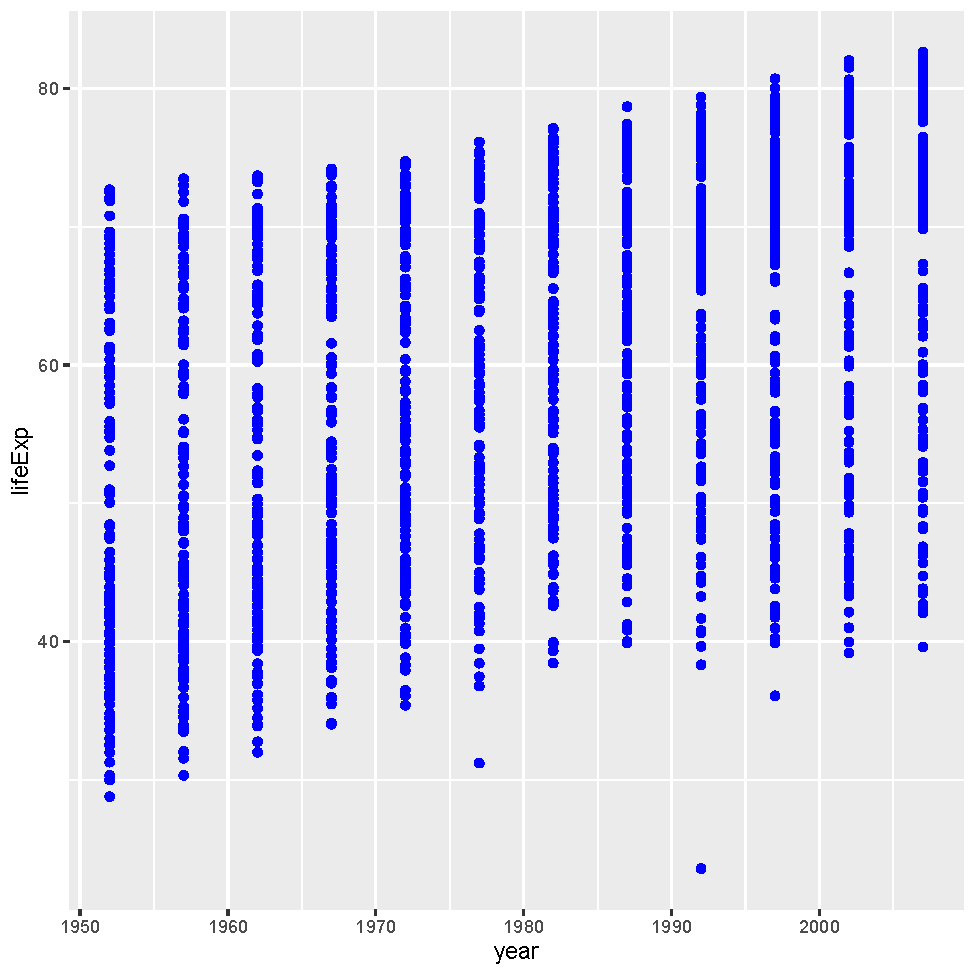
\includegraphics[width=0.7\linewidth,keepaspectratio]{Multivariable_Data_Analysis_files/figure-latex/unnamed-chunk-21-1} \end{center}

And then parameter shape to plus (which is represented by number 3).

\begin{Shaded}
\begin{Highlighting}[]
\FunctionTok{ggplot}\NormalTok{(}\AttributeTok{data =}\NormalTok{ gapminder) }\SpecialCharTok{+}
  \FunctionTok{geom\_point}\NormalTok{(}\AttributeTok{mapping =} \FunctionTok{aes}\NormalTok{(}\AttributeTok{x =}\NormalTok{ year, }\AttributeTok{y =}\NormalTok{ lifeExp), }\AttributeTok{shape =} \DecValTok{3}\NormalTok{)}
\end{Highlighting}
\end{Shaded}

\begin{center}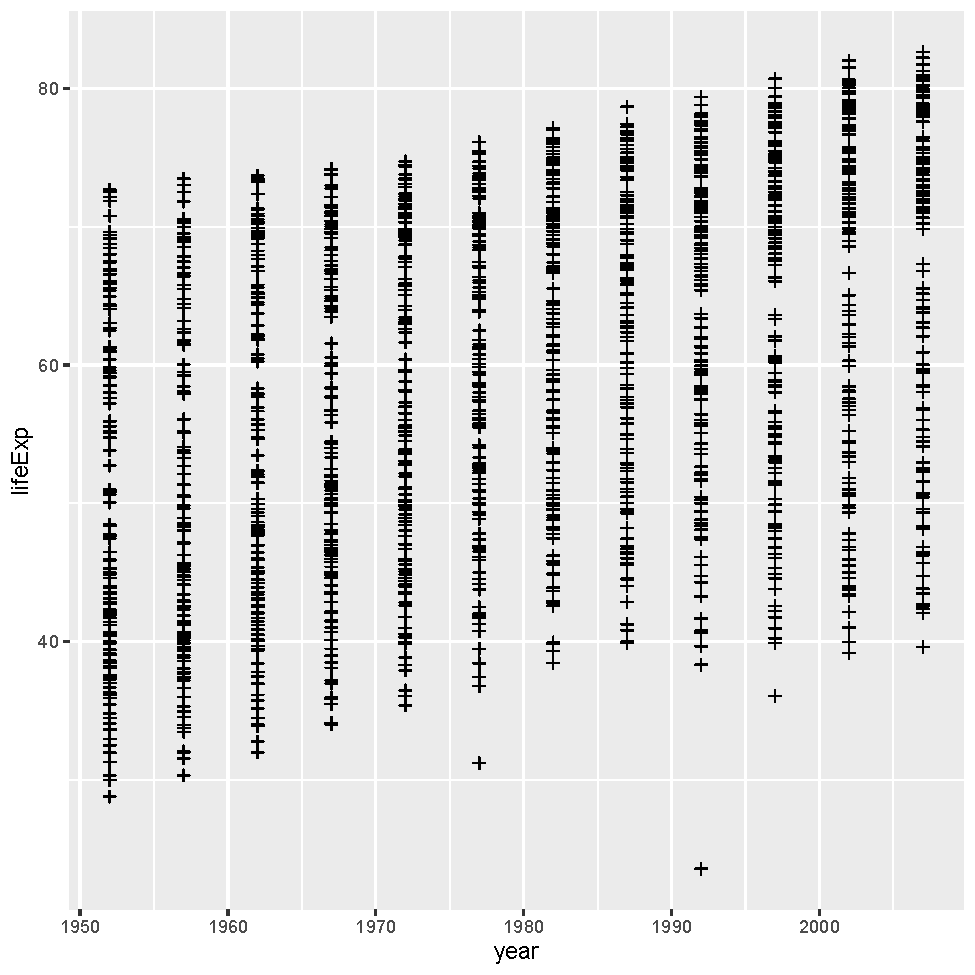
\includegraphics[width=0.7\linewidth,keepaspectratio]{Multivariable_Data_Analysis_files/figure-latex/unnamed-chunk-22-1} \end{center}

You may wonder what number corresponds to what type of shape. You can type \(?pch\). And you will see in the Viewer pane, the explanation about the shape available in R. It also shows what number that corresponds to what shape.

\hypertarget{making-subplots}{%
\section{Making subplots}\label{making-subplots}}

We can split our plots based on a factor variable and make subplots using the \texttt{facet()}. For example, if we want to make subplots based on continents, then you need to set these parameters:

\begin{itemize}
\tightlist
\item
  data = gapminder
\item
  variable year on the x-axis and lifeExp on the y-axis
\item
  split the plot based on continent
\item
  the number of rows for the plot are 3
\end{itemize}

\begin{Shaded}
\begin{Highlighting}[]
\FunctionTok{ggplot}\NormalTok{(}\AttributeTok{data =}\NormalTok{ gapminder) }\SpecialCharTok{+}
  \FunctionTok{geom\_point}\NormalTok{(}\AttributeTok{mapping =} \FunctionTok{aes}\NormalTok{(}\AttributeTok{x =}\NormalTok{ year, }\AttributeTok{y =}\NormalTok{ lifeExp)) }\SpecialCharTok{+} 
  \FunctionTok{facet\_wrap}\NormalTok{(}\SpecialCharTok{\textasciitilde{}}\NormalTok{ continent, }\AttributeTok{nrow =} \DecValTok{3}\NormalTok{)}
\end{Highlighting}
\end{Shaded}

\begin{center}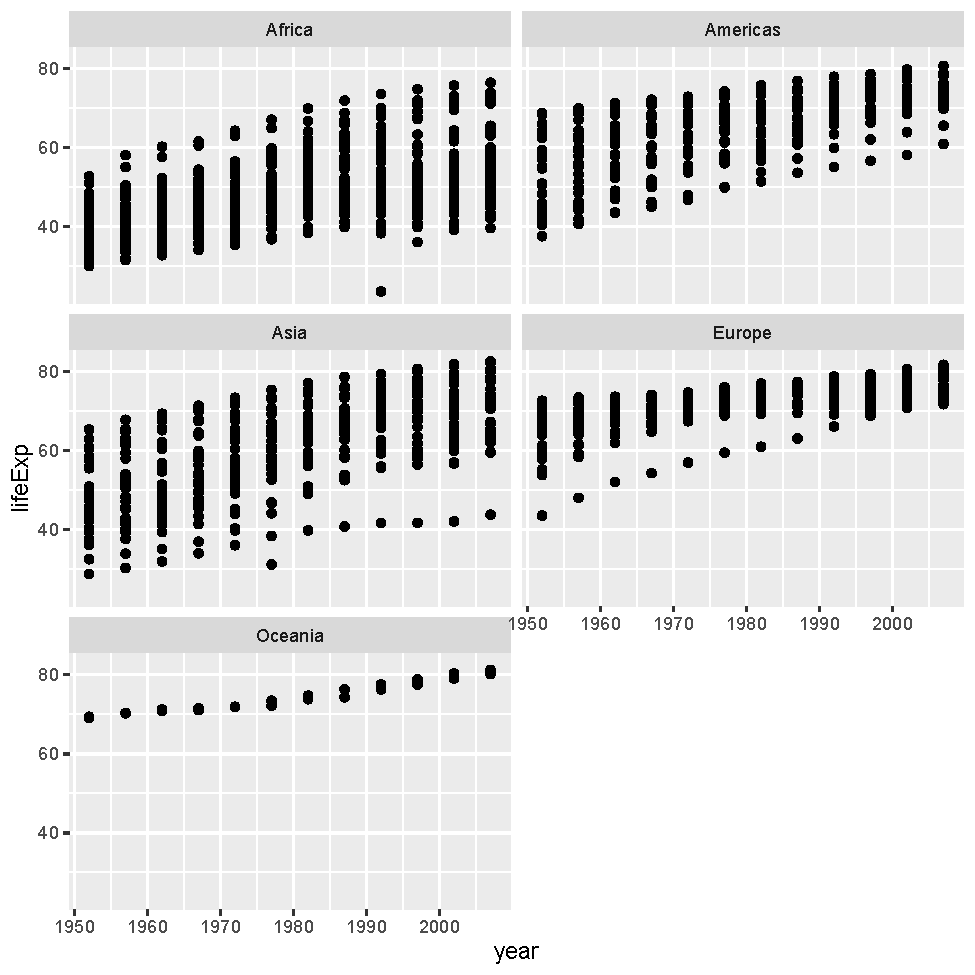
\includegraphics[width=0.7\linewidth,keepaspectratio]{Multivariable_Data_Analysis_files/figure-latex/unnamed-chunk-23-1} \end{center}

Now, what happen if we change the value for the nrow

\begin{Shaded}
\begin{Highlighting}[]
\FunctionTok{ggplot}\NormalTok{(}\AttributeTok{data =}\NormalTok{ gapminder) }\SpecialCharTok{+}
  \FunctionTok{geom\_point}\NormalTok{(}\AttributeTok{mapping =} \FunctionTok{aes}\NormalTok{(}\AttributeTok{x =}\NormalTok{ year, }\AttributeTok{y =}\NormalTok{ lifeExp)) }\SpecialCharTok{+} 
  \FunctionTok{facet\_wrap}\NormalTok{(}\SpecialCharTok{\textasciitilde{}}\NormalTok{ continent, }\AttributeTok{nrow =} \DecValTok{2}\NormalTok{)}
\end{Highlighting}
\end{Shaded}

\begin{center}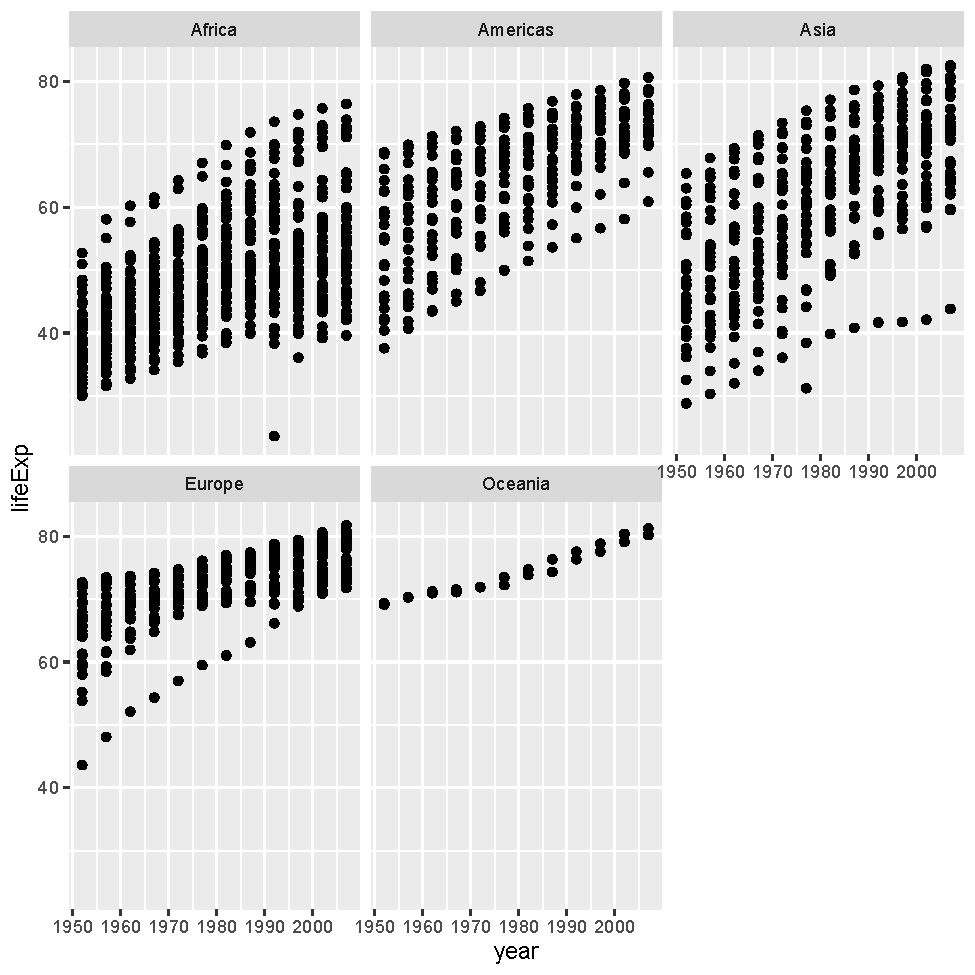
\includegraphics[width=0.7\linewidth,keepaspectratio]{Multivariable_Data_Analysis_files/figure-latex/unnamed-chunk-24-1} \end{center}

\hypertarget{overlaying-plots}{%
\section{Overlaying plots}\label{overlaying-plots}}

Each \texttt{geom\_X()} in ggplot2 indicates different visual objects.

This is a scatterplot

\begin{Shaded}
\begin{Highlighting}[]
\FunctionTok{ggplot}\NormalTok{(}\AttributeTok{data =}\NormalTok{ gapminder) }\SpecialCharTok{+}
  \FunctionTok{geom\_point}\NormalTok{(}\AttributeTok{mapping =} \FunctionTok{aes}\NormalTok{(}\AttributeTok{x =}\NormalTok{ gdpPercap, }\AttributeTok{y =}\NormalTok{ lifeExp))}
\end{Highlighting}
\end{Shaded}

\begin{center}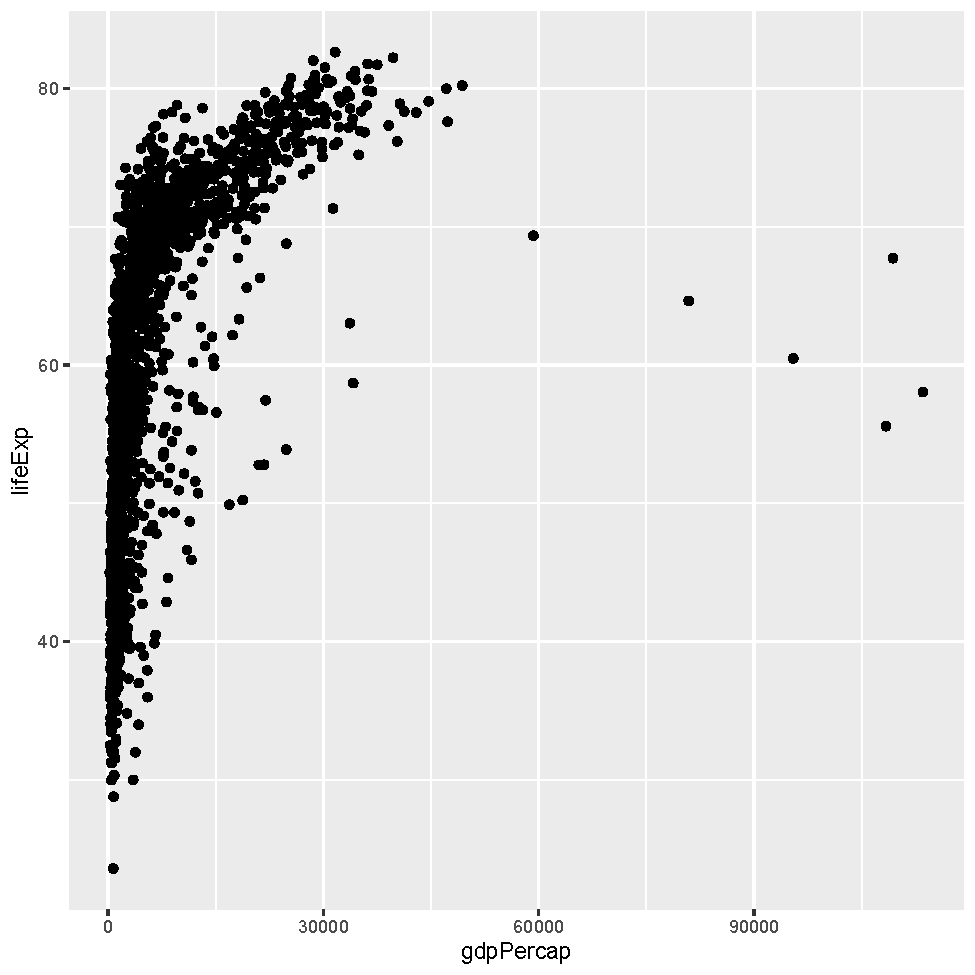
\includegraphics[width=0.7\linewidth,keepaspectratio]{Multivariable_Data_Analysis_files/figure-latex/unnamed-chunk-25-1} \end{center}

This is a smooth line

\begin{Shaded}
\begin{Highlighting}[]
\FunctionTok{ggplot}\NormalTok{(}\AttributeTok{data =}\NormalTok{ gapminder) }\SpecialCharTok{+}
  \FunctionTok{geom\_smooth}\NormalTok{(}\AttributeTok{mapping =} \FunctionTok{aes}\NormalTok{(}\AttributeTok{x =}\NormalTok{ gdpPercap, }\AttributeTok{y =}\NormalTok{ lifeExp))}
\end{Highlighting}
\end{Shaded}

\begin{center}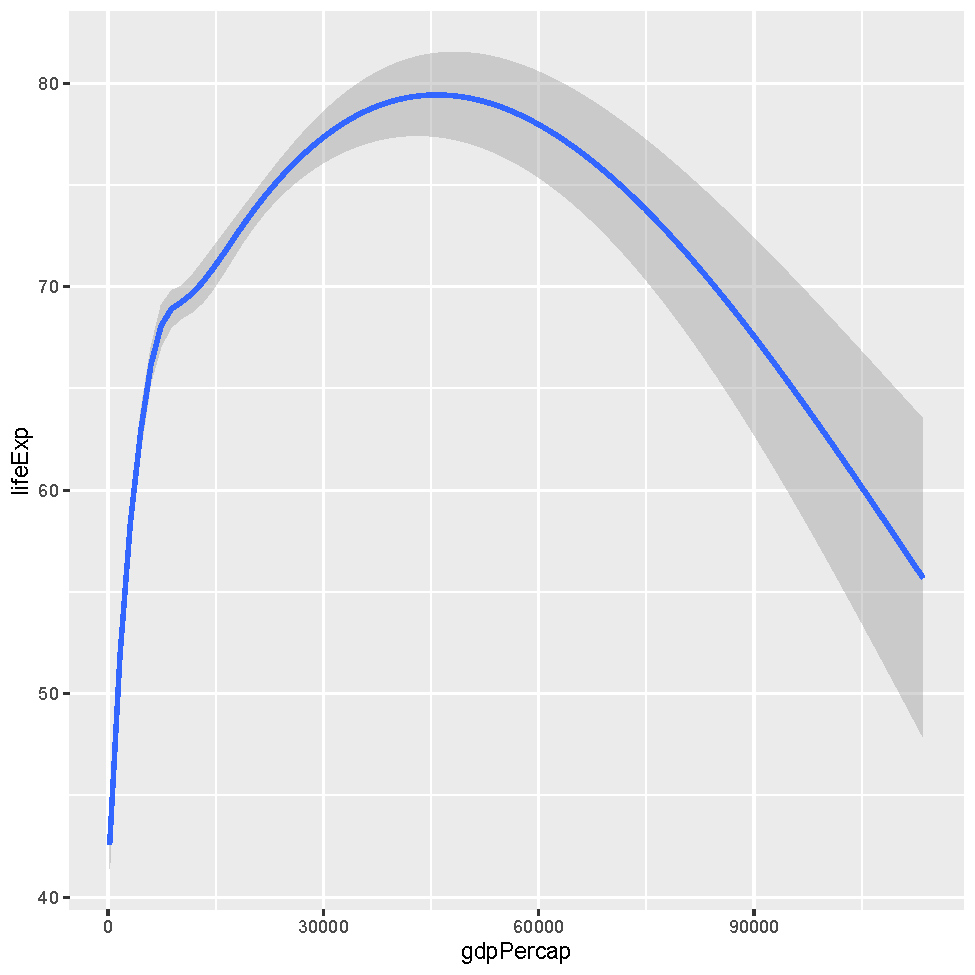
\includegraphics[width=0.7\linewidth,keepaspectratio]{Multivariable_Data_Analysis_files/figure-latex/unnamed-chunk-26-1} \end{center}

And we can regenerate the smooth plot based on continent using the \texttt{linetype()}. We use \texttt{log(gdpPercap)} to reduce the skewness of the data.

\begin{Shaded}
\begin{Highlighting}[]
\FunctionTok{ggplot}\NormalTok{(}\AttributeTok{data =}\NormalTok{ gapminder) }\SpecialCharTok{+}
  \FunctionTok{geom\_smooth}\NormalTok{(}\AttributeTok{mapping =} \FunctionTok{aes}\NormalTok{(}\AttributeTok{x =} \FunctionTok{log}\NormalTok{(gdpPercap), }\AttributeTok{y =}\NormalTok{ lifeExp, }\AttributeTok{linetype =}\NormalTok{ continent))}
\end{Highlighting}
\end{Shaded}

\begin{center}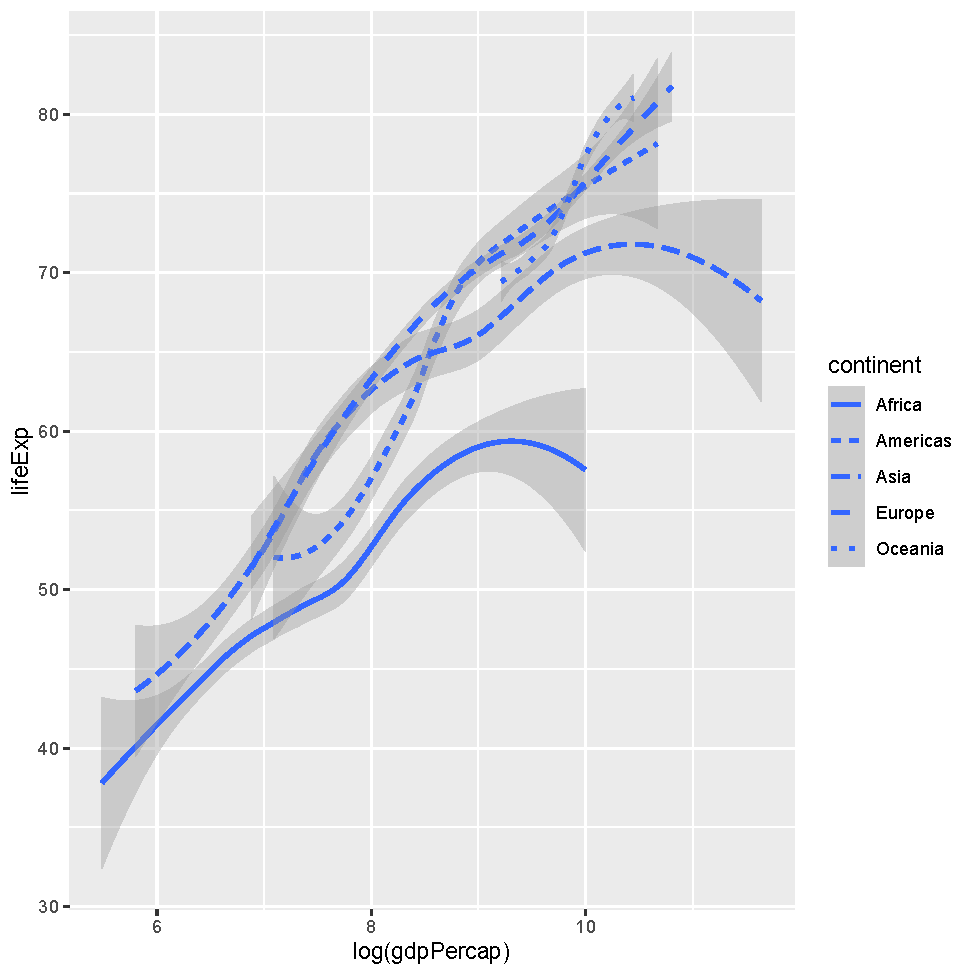
\includegraphics[width=0.7\linewidth,keepaspectratio]{Multivariable_Data_Analysis_files/figure-latex/unnamed-chunk-27-1} \end{center}

Another smooth plot but setting the parameter for colour

\begin{Shaded}
\begin{Highlighting}[]
\FunctionTok{ggplot}\NormalTok{(}\AttributeTok{data =}\NormalTok{ gapminder) }\SpecialCharTok{+}
  \FunctionTok{geom\_smooth}\NormalTok{(}\AttributeTok{mapping =} \FunctionTok{aes}\NormalTok{(}\AttributeTok{x =} \FunctionTok{log}\NormalTok{(gdpPercap), }\AttributeTok{y =}\NormalTok{ lifeExp, }\AttributeTok{colour =}\NormalTok{ continent))}
\end{Highlighting}
\end{Shaded}

\begin{center}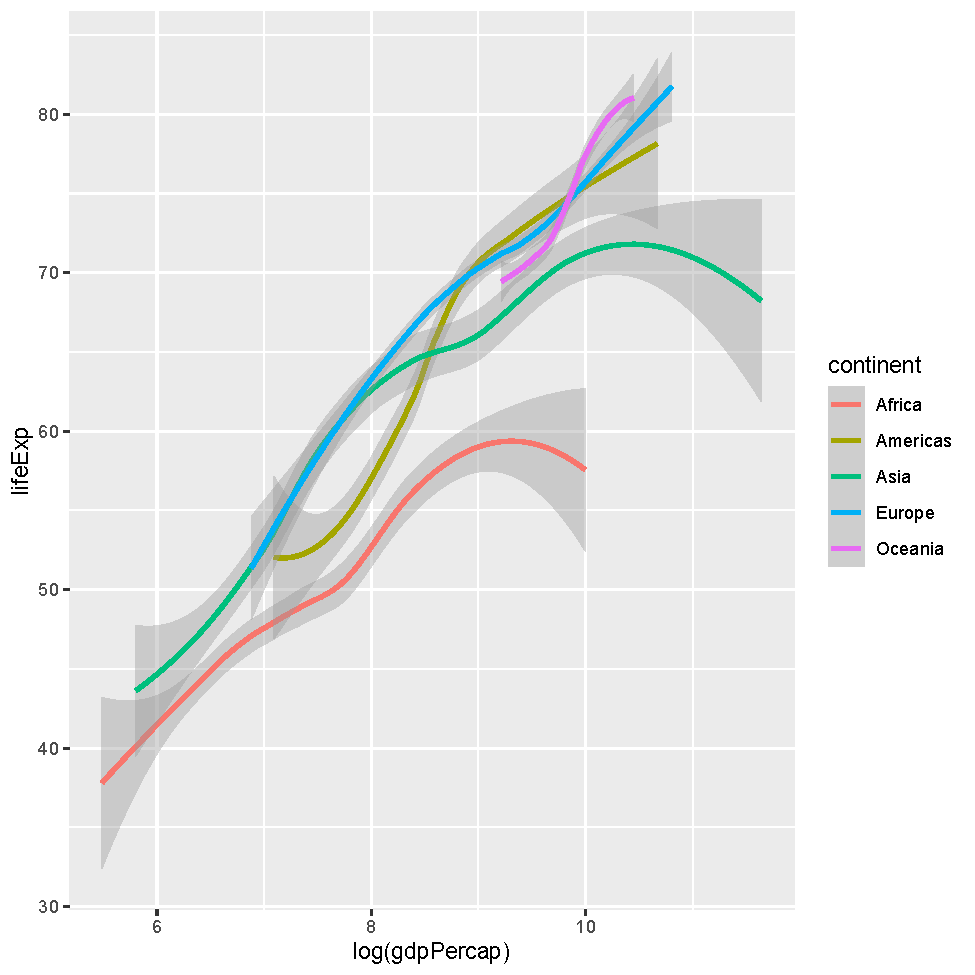
\includegraphics[width=0.7\linewidth,keepaspectratio]{Multivariable_Data_Analysis_files/figure-latex/unnamed-chunk-28-1} \end{center}

\hypertarget{combining-geom}{%
\section{Combining geom}\label{combining-geom}}

We can combine more than one geoms to overlay plots. The trick is to use multiple geoms in a single line of R code

\begin{Shaded}
\begin{Highlighting}[]
\FunctionTok{ggplot}\NormalTok{(}\AttributeTok{data =}\NormalTok{ gapminder) }\SpecialCharTok{+}
  \FunctionTok{geom\_point}\NormalTok{(}\AttributeTok{mapping =} \FunctionTok{aes}\NormalTok{(}\AttributeTok{x =} \FunctionTok{log}\NormalTok{(gdpPercap), }\AttributeTok{y =}\NormalTok{ lifeExp)) }\SpecialCharTok{+}
  \FunctionTok{geom\_smooth}\NormalTok{(}\AttributeTok{mapping =} \FunctionTok{aes}\NormalTok{(}\AttributeTok{x =} \FunctionTok{log}\NormalTok{(gdpPercap), }\AttributeTok{y =}\NormalTok{ lifeExp))}
\end{Highlighting}
\end{Shaded}

\begin{center}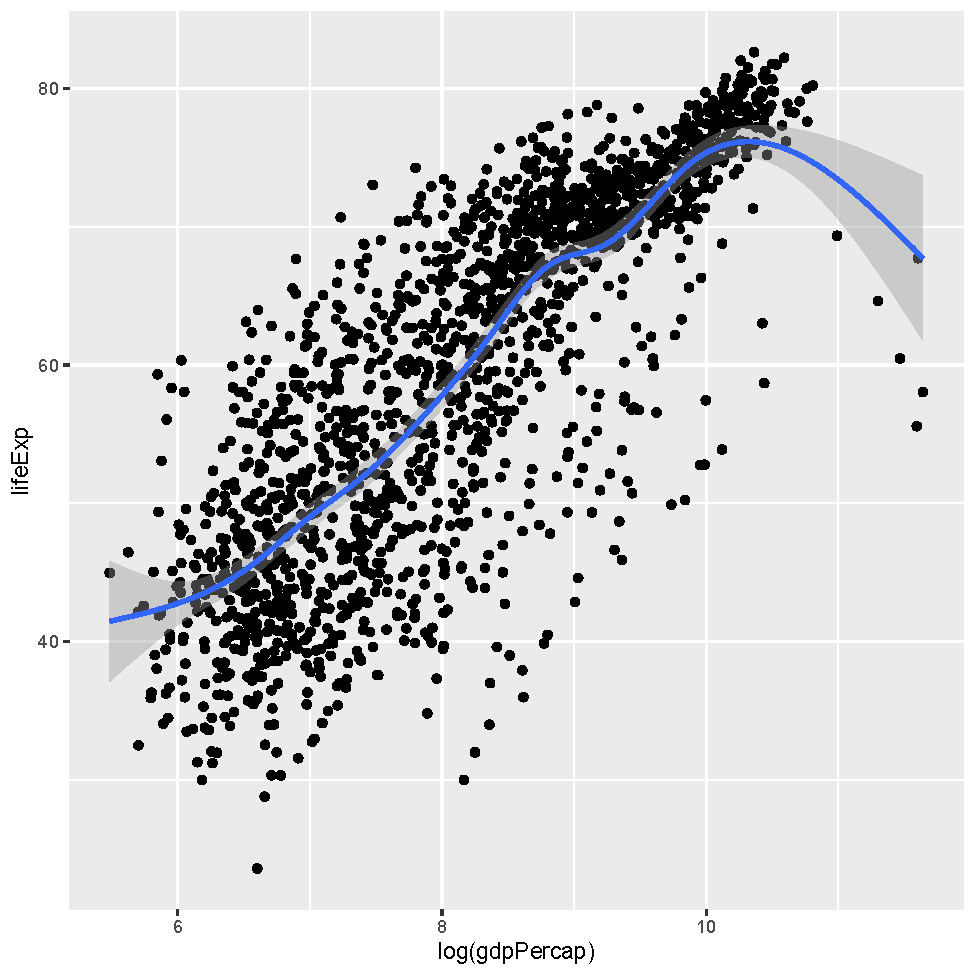
\includegraphics[width=0.7\linewidth,keepaspectratio]{Multivariable_Data_Analysis_files/figure-latex/unnamed-chunk-29-1} \end{center}

The codes above show duplication or repetition. To avoid this, we can pass the mapping to \texttt{ggplot()}.

\begin{Shaded}
\begin{Highlighting}[]
\FunctionTok{ggplot}\NormalTok{(}\AttributeTok{data =}\NormalTok{ gapminder, }\AttributeTok{mapping =} \FunctionTok{aes}\NormalTok{(}\AttributeTok{x =} \FunctionTok{log}\NormalTok{(gdpPercap), }\AttributeTok{y =}\NormalTok{ lifeExp)) }\SpecialCharTok{+}
  \FunctionTok{geom\_point}\NormalTok{() }\SpecialCharTok{+}
  \FunctionTok{geom\_smooth}\NormalTok{()}
\end{Highlighting}
\end{Shaded}

\begin{center}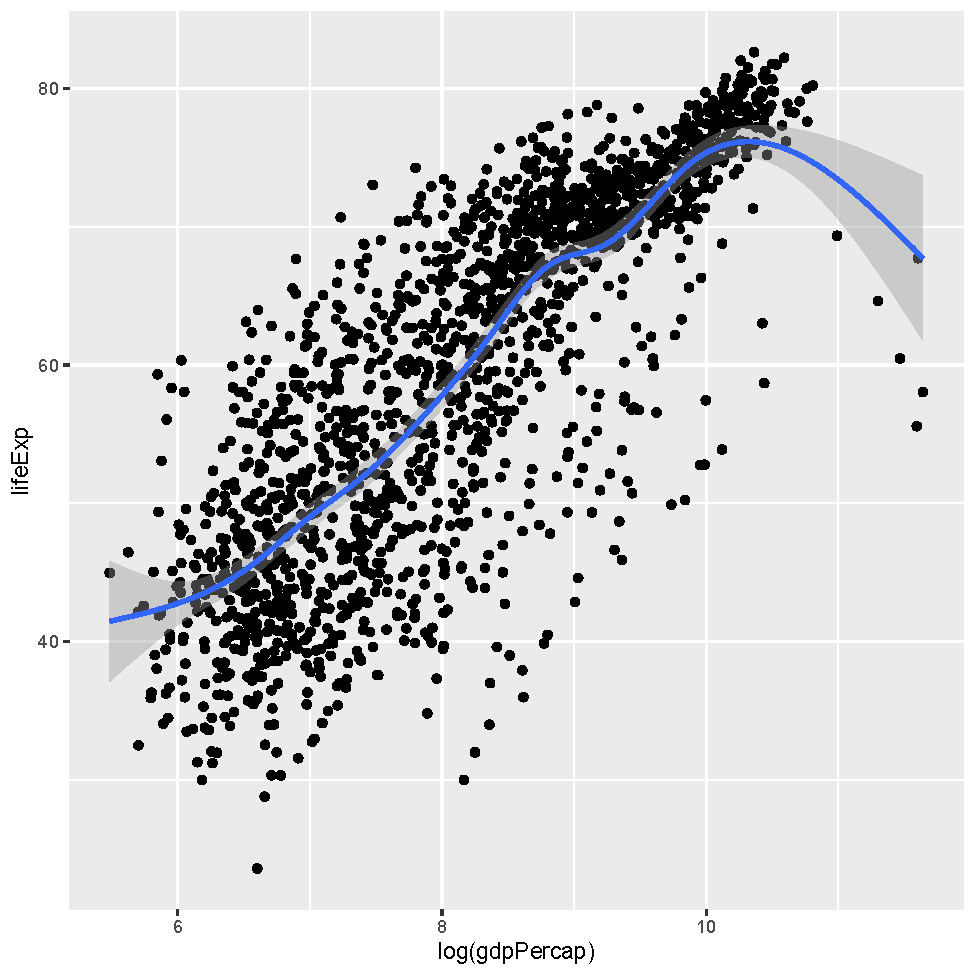
\includegraphics[width=0.7\linewidth,keepaspectratio]{Multivariable_Data_Analysis_files/figure-latex/unnamed-chunk-30-1} \end{center}

And we can expand this to make scatterplot shows different colour for continent

\begin{Shaded}
\begin{Highlighting}[]
\FunctionTok{ggplot}\NormalTok{(}\AttributeTok{data =}\NormalTok{ gapminder, }\AttributeTok{mapping =} \FunctionTok{aes}\NormalTok{(}\AttributeTok{x =} \FunctionTok{log}\NormalTok{(gdpPercap), }\AttributeTok{y =}\NormalTok{ lifeExp)) }\SpecialCharTok{+}
  \FunctionTok{geom\_point}\NormalTok{(}\AttributeTok{mapping =} \FunctionTok{aes}\NormalTok{(}\AttributeTok{colour =}\NormalTok{ continent)) }\SpecialCharTok{+}
  \FunctionTok{geom\_smooth}\NormalTok{()}
\end{Highlighting}
\end{Shaded}

\begin{center}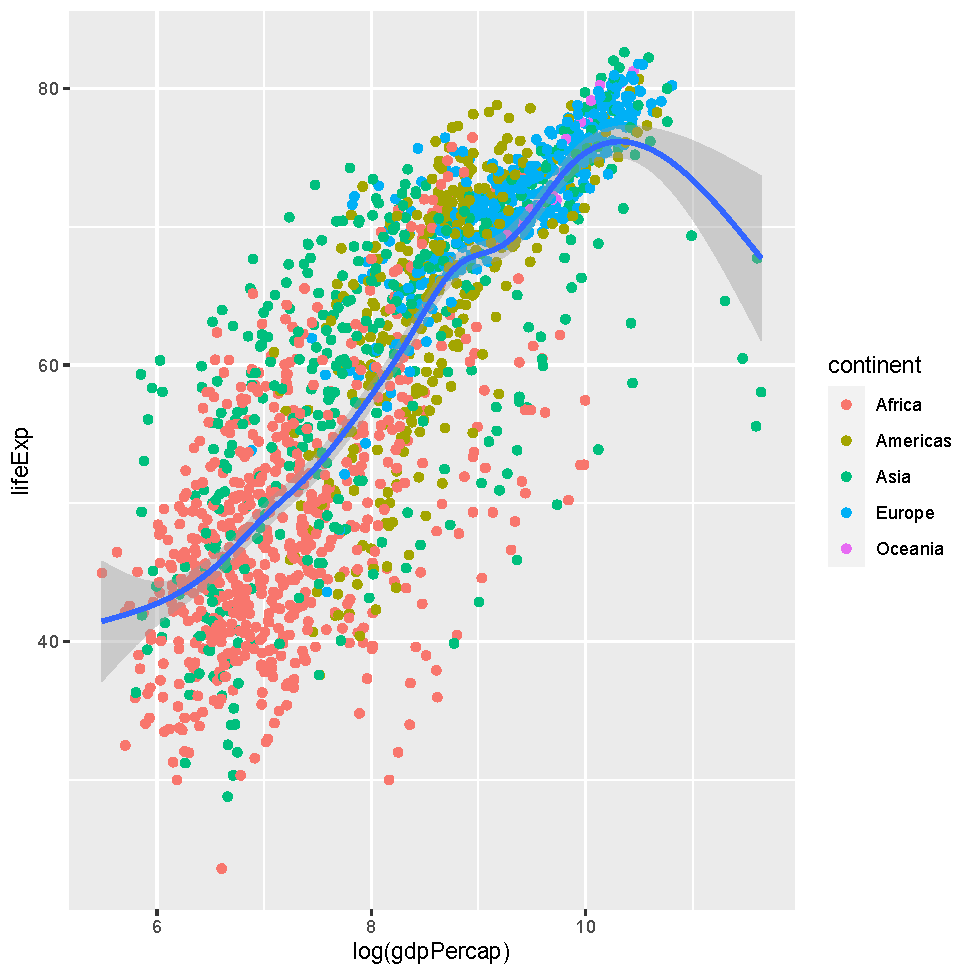
\includegraphics[width=0.7\linewidth,keepaspectratio]{Multivariable_Data_Analysis_files/figure-latex/unnamed-chunk-31-1} \end{center}

Or expand this to make the smooth plot shows different colour for continent

\begin{Shaded}
\begin{Highlighting}[]
\FunctionTok{ggplot}\NormalTok{(}\AttributeTok{data =}\NormalTok{ gapminder, }\AttributeTok{mapping =} \FunctionTok{aes}\NormalTok{(}\AttributeTok{x =} \FunctionTok{log}\NormalTok{(gdpPercap), }\AttributeTok{y =}\NormalTok{ lifeExp)) }\SpecialCharTok{+}
  \FunctionTok{geom\_point}\NormalTok{() }\SpecialCharTok{+}
  \FunctionTok{geom\_smooth}\NormalTok{(}\AttributeTok{mapping =} \FunctionTok{aes}\NormalTok{(}\AttributeTok{colour =}\NormalTok{ continent))}
\end{Highlighting}
\end{Shaded}

\begin{center}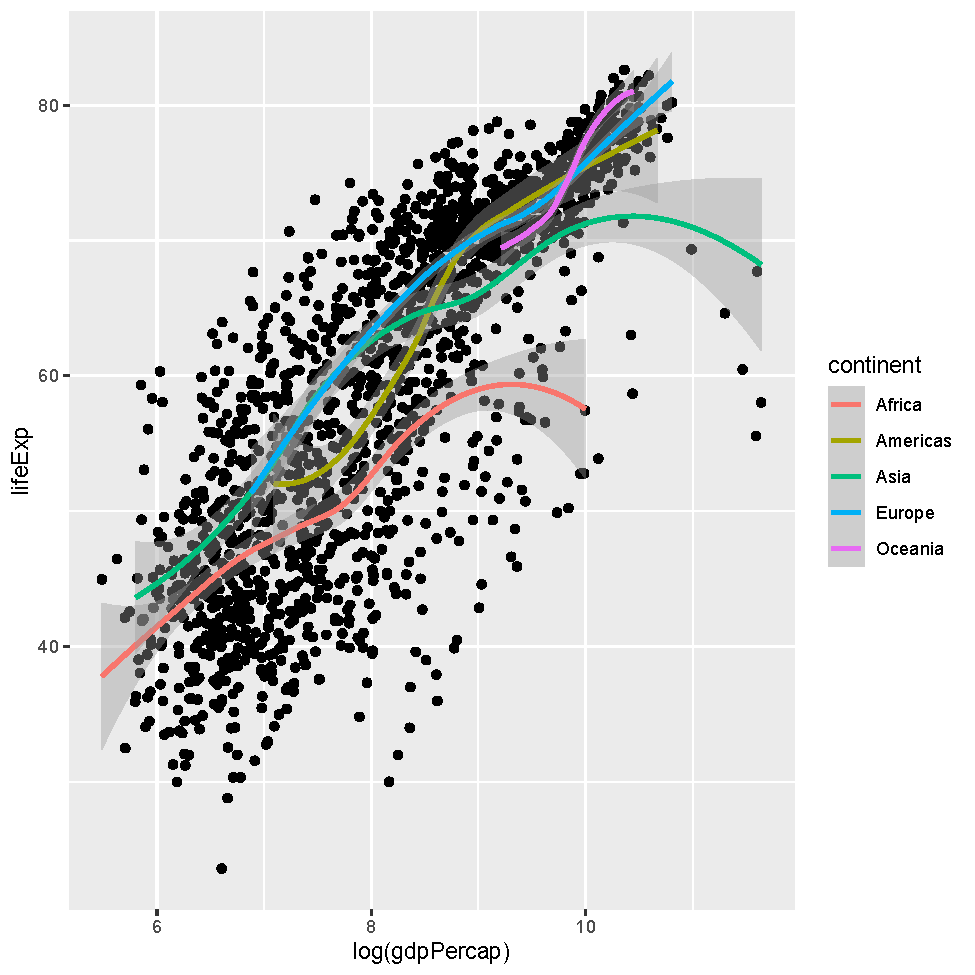
\includegraphics[width=0.7\linewidth,keepaspectratio]{Multivariable_Data_Analysis_files/figure-latex/unnamed-chunk-32-1} \end{center}

Or both the scatterplot and the smoothplot

\begin{Shaded}
\begin{Highlighting}[]
\FunctionTok{ggplot}\NormalTok{(}\AttributeTok{data =}\NormalTok{ gapminder, }\AttributeTok{mapping =} \FunctionTok{aes}\NormalTok{(}\AttributeTok{x =} \FunctionTok{log}\NormalTok{(gdpPercap), }\AttributeTok{y =}\NormalTok{ lifeExp)) }\SpecialCharTok{+}
  \FunctionTok{geom\_point}\NormalTok{(}\AttributeTok{mapping =} \FunctionTok{aes}\NormalTok{(}\AttributeTok{shape =}\NormalTok{ continent)) }\SpecialCharTok{+}
  \FunctionTok{geom\_smooth}\NormalTok{(}\AttributeTok{mapping =} \FunctionTok{aes}\NormalTok{(}\AttributeTok{colour =}\NormalTok{ continent))}
\end{Highlighting}
\end{Shaded}

\begin{center}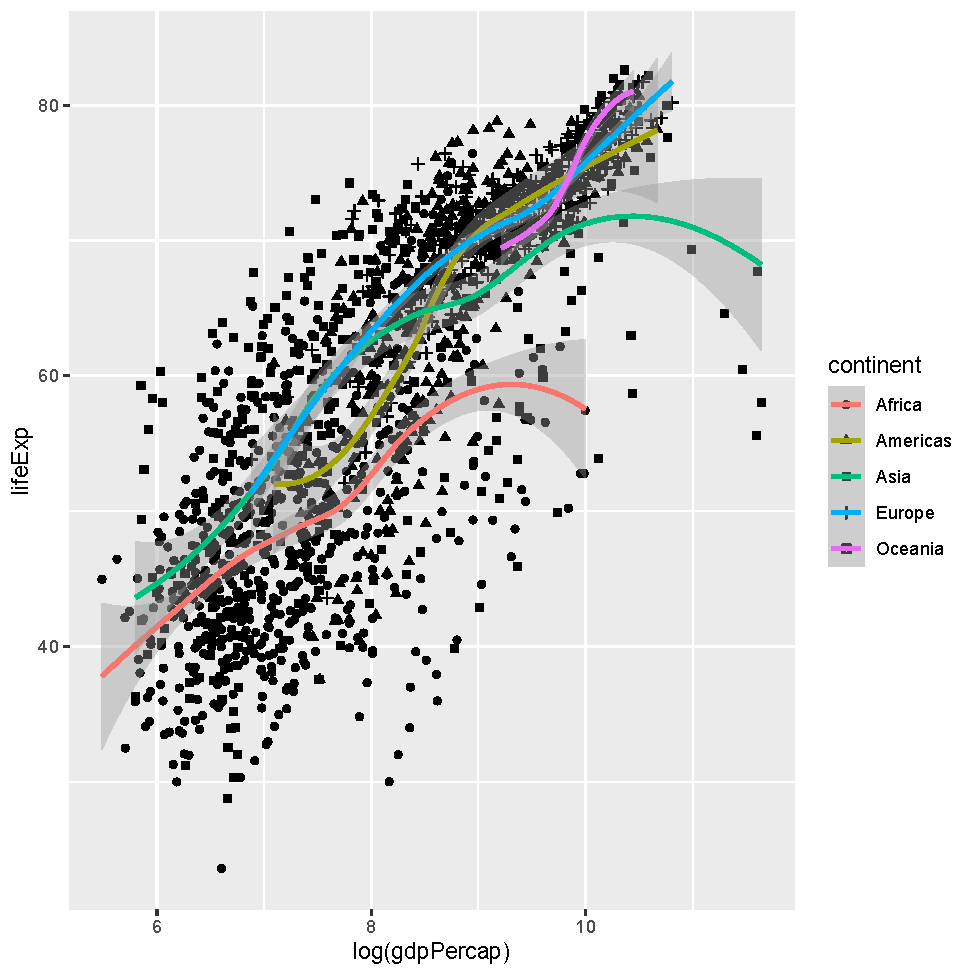
\includegraphics[width=0.7\linewidth,keepaspectratio]{Multivariable_Data_Analysis_files/figure-latex/unnamed-chunk-33-1} \end{center}

\hypertarget{statistical-transformation}{%
\section{Statistical transformation}\label{statistical-transformation}}

Let us create a bar chart, with y axis as the frequency.

\begin{Shaded}
\begin{Highlighting}[]
\FunctionTok{ggplot}\NormalTok{(}\AttributeTok{data =}\NormalTok{ gapminder) }\SpecialCharTok{+}
  \FunctionTok{geom\_bar}\NormalTok{(}\AttributeTok{mapping =} \FunctionTok{aes}\NormalTok{(}\AttributeTok{x =}\NormalTok{ continent))}
\end{Highlighting}
\end{Shaded}

\begin{center}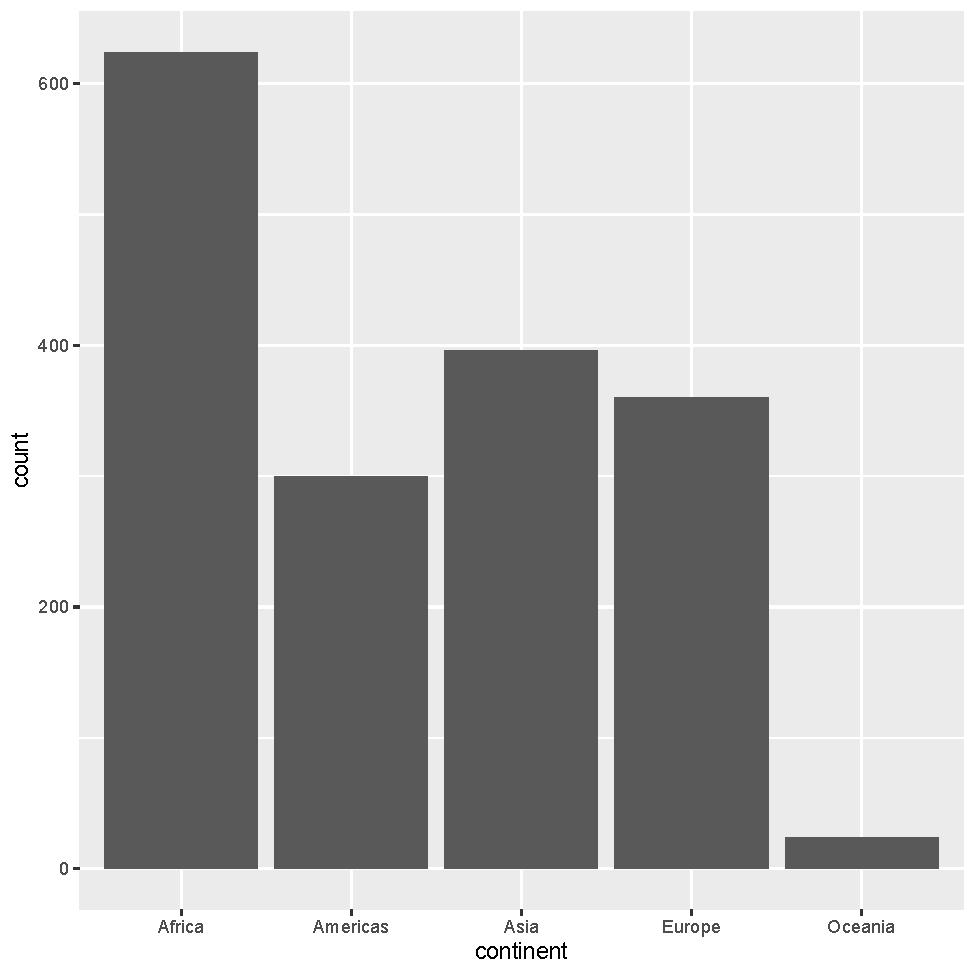
\includegraphics[width=0.7\linewidth,keepaspectratio]{Multivariable_Data_Analysis_files/figure-latex/unnamed-chunk-34-1} \end{center}

If we want the y-axis to show proportion, we can use these codes

\begin{Shaded}
\begin{Highlighting}[]
\FunctionTok{ggplot}\NormalTok{(}\AttributeTok{data =}\NormalTok{ gapminder) }\SpecialCharTok{+}
  \FunctionTok{geom\_bar}\NormalTok{(}\AttributeTok{mapping =} \FunctionTok{aes}\NormalTok{(}\AttributeTok{x =}\NormalTok{ continent, }\AttributeTok{y =}\NormalTok{ ..prop..,}
                         \AttributeTok{group =} \DecValTok{1}\NormalTok{))}
\end{Highlighting}
\end{Shaded}

\begin{center}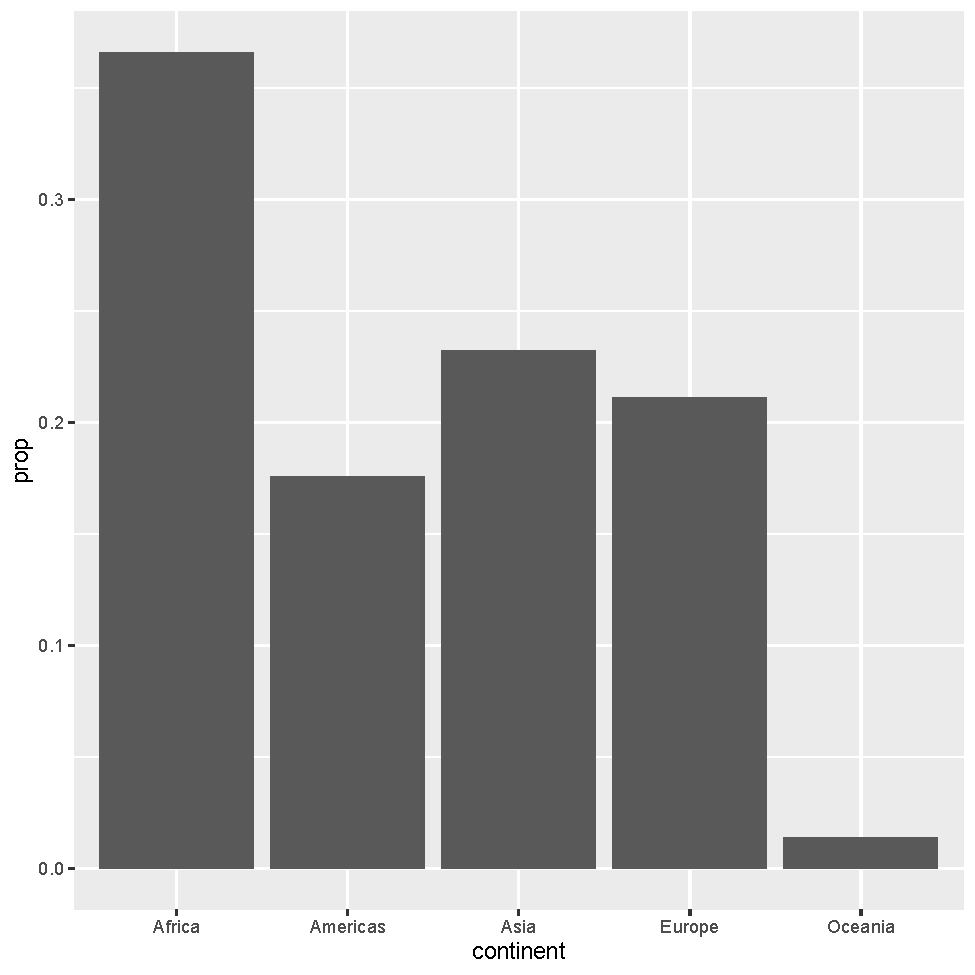
\includegraphics[width=0.7\linewidth,keepaspectratio]{Multivariable_Data_Analysis_files/figure-latex/unnamed-chunk-35-1} \end{center}

\hypertarget{customizing-title}{%
\section{Customizing title}\label{customizing-title}}

We can customize many aspects of the plot using ggplot package. For example, from gapminder dataset, we choose GDP and log it (to reduce skewness) and life expectancy, and make a scatterplot. We named the plot as \texttt{my\_pop}

\begin{Shaded}
\begin{Highlighting}[]
\NormalTok{mypop }\OtherTok{\textless{}{-}} \FunctionTok{ggplot}\NormalTok{(}\AttributeTok{data =}\NormalTok{ gapminder, }\AttributeTok{mapping =} \FunctionTok{aes}\NormalTok{(}\AttributeTok{x =} \FunctionTok{log}\NormalTok{(gdpPercap), }\AttributeTok{y =}\NormalTok{ lifeExp)) }\SpecialCharTok{+}
  \FunctionTok{geom\_point}\NormalTok{() }\SpecialCharTok{+}
  \FunctionTok{geom\_smooth}\NormalTok{(}\AttributeTok{mapping =} \FunctionTok{aes}\NormalTok{(}\AttributeTok{colour =}\NormalTok{ continent))}
\NormalTok{mypop}
\end{Highlighting}
\end{Shaded}

\begin{center}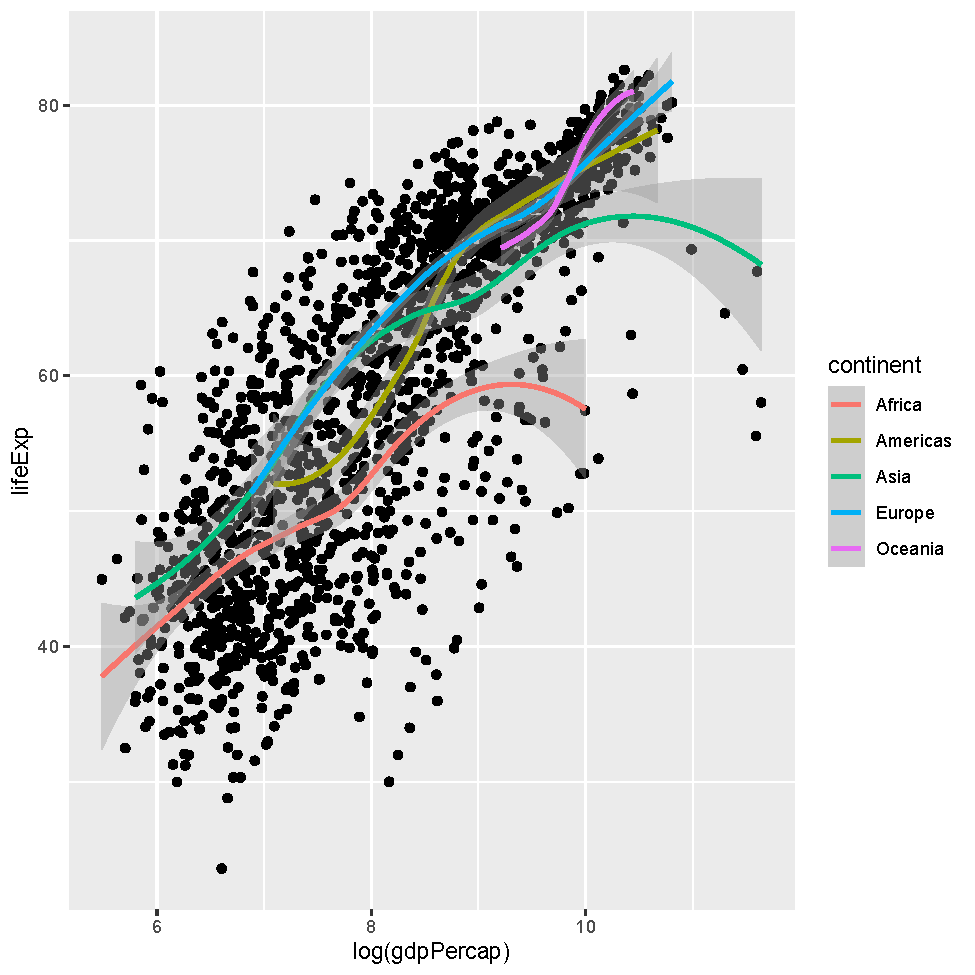
\includegraphics[width=0.7\linewidth,keepaspectratio]{Multivariable_Data_Analysis_files/figure-latex/unnamed-chunk-36-1} \end{center}

You will notice that there is no title in the plot. A title can be added to the plot.

\begin{Shaded}
\begin{Highlighting}[]
\NormalTok{mypop }\SpecialCharTok{+} \FunctionTok{ggtitle}\NormalTok{(}\StringTok{"Scatterplot showing the relationship of GDP in log and life expectancy"}\NormalTok{)}
\end{Highlighting}
\end{Shaded}

\begin{center}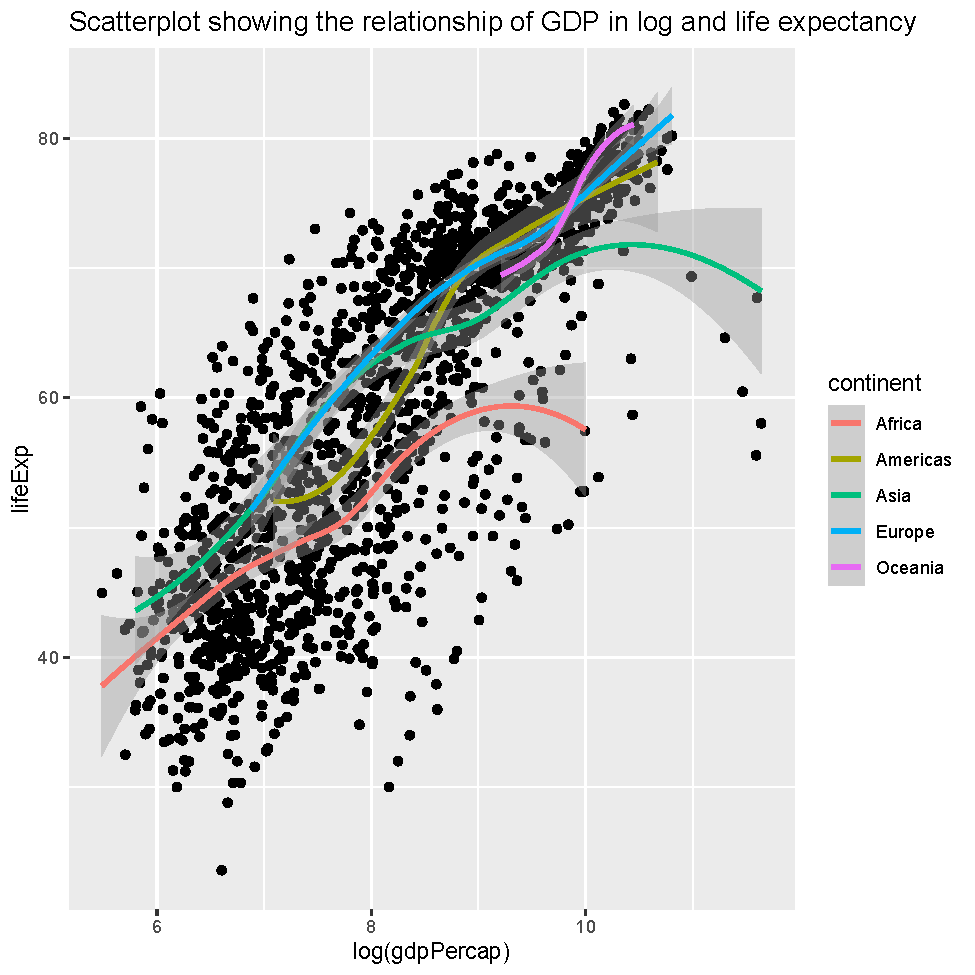
\includegraphics[width=0.7\linewidth,keepaspectratio]{Multivariable_Data_Analysis_files/figure-latex/unnamed-chunk-37-1} \end{center}

Title in multiple lines by adding \texttt{\textbackslash{}n}

\begin{Shaded}
\begin{Highlighting}[]
\NormalTok{mypop }\SpecialCharTok{+} \FunctionTok{ggtitle}\NormalTok{(}\StringTok{"Scatterplot showing the relationship of GDP in log and life expectancy:}
\StringTok{                }\SpecialCharTok{\textbackslash{}n}\StringTok{Data from Gapminder"}\NormalTok{)}
\end{Highlighting}
\end{Shaded}

\begin{center}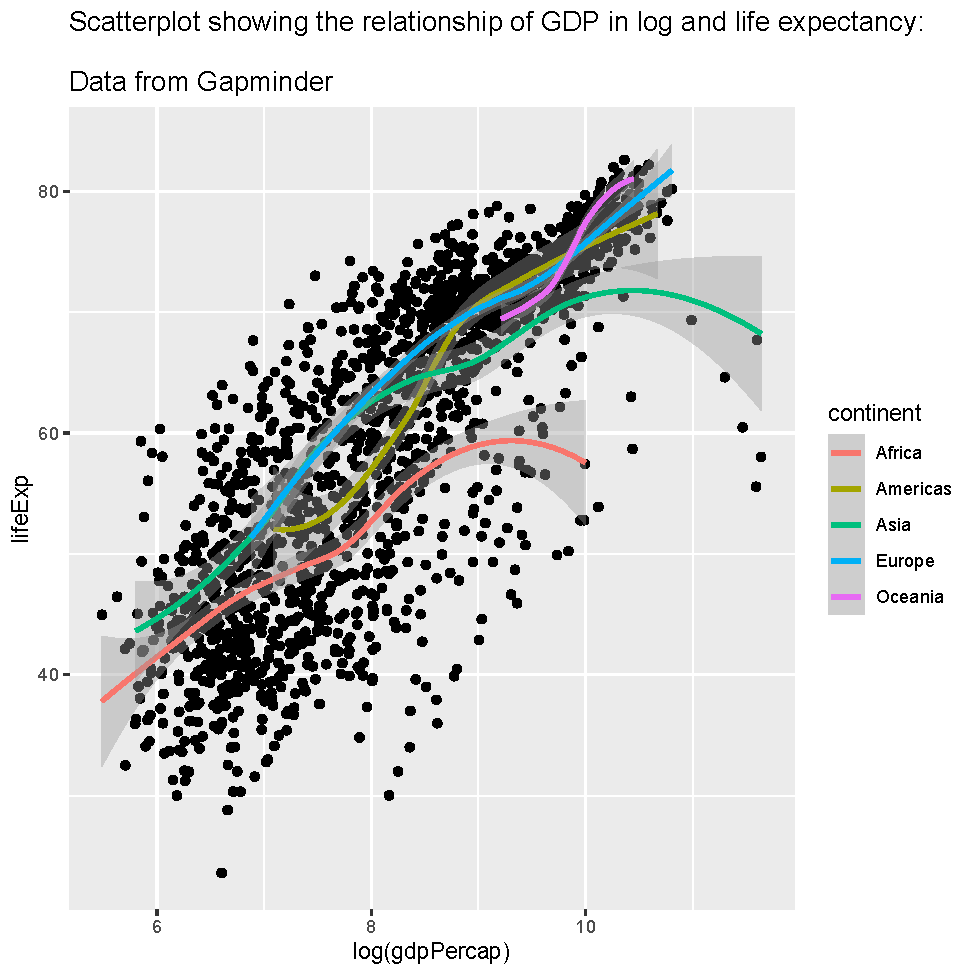
\includegraphics[width=0.7\linewidth,keepaspectratio]{Multivariable_Data_Analysis_files/figure-latex/unnamed-chunk-38-1} \end{center}

\hypertarget{adjusting-axes}{%
\section{Adjusting axes}\label{adjusting-axes}}

We can specify the tick marks

\begin{enumerate}
\def\labelenumi{\arabic{enumi}.}
\tightlist
\item
  min = 0
\item
  max = 12
\item
  interval = 1
\end{enumerate}

\begin{Shaded}
\begin{Highlighting}[]
\NormalTok{mypop }\SpecialCharTok{+} \FunctionTok{scale\_x\_continuous}\NormalTok{(}\AttributeTok{breaks =} \FunctionTok{seq}\NormalTok{(}\DecValTok{0}\NormalTok{,}\DecValTok{12}\NormalTok{,}\DecValTok{1}\NormalTok{))}
\end{Highlighting}
\end{Shaded}

\begin{center}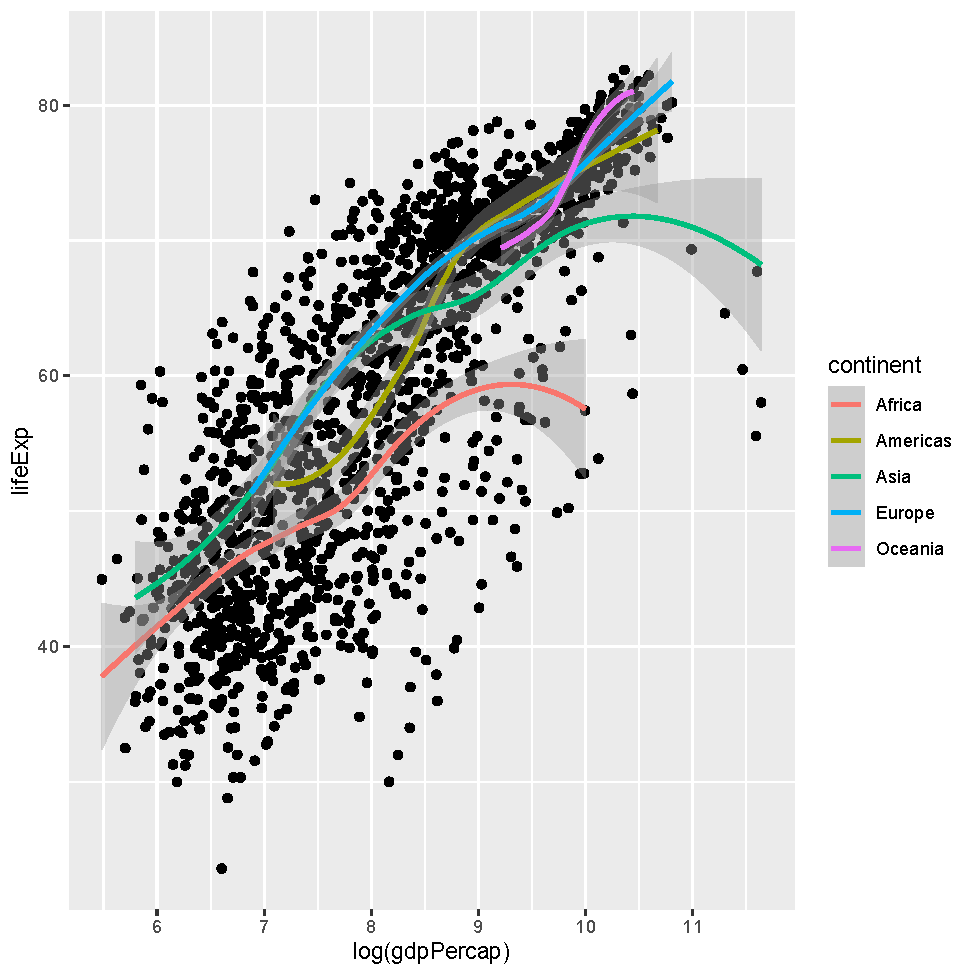
\includegraphics[width=0.7\linewidth,keepaspectratio]{Multivariable_Data_Analysis_files/figure-latex/unnamed-chunk-39-1} \end{center}

And we can label the x-axis and y-axis

\begin{Shaded}
\begin{Highlighting}[]
\NormalTok{mypop }\SpecialCharTok{+} \FunctionTok{ggtitle}\NormalTok{(}\StringTok{"Scatterplot showing the relationship of GDP in log and life expectancy:}
\StringTok{                }\SpecialCharTok{\textbackslash{}n}\StringTok{Data from Gapminder"}\NormalTok{) }\SpecialCharTok{+} \FunctionTok{ylab}\NormalTok{(}\StringTok{"Life Expentancy"}\NormalTok{) }\SpecialCharTok{+} \FunctionTok{xlab}\NormalTok{(}\StringTok{"Percapita GDP in log"}\NormalTok{)}
\end{Highlighting}
\end{Shaded}

\begin{center}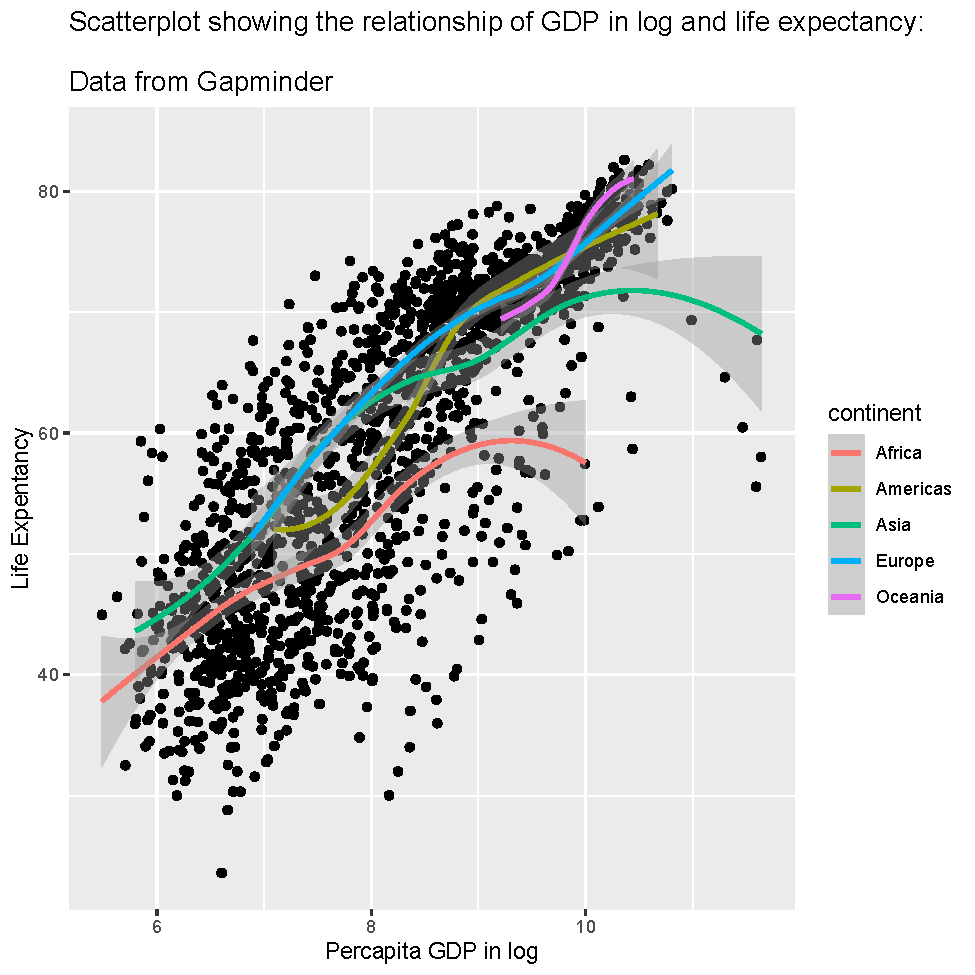
\includegraphics[width=0.7\linewidth,keepaspectratio]{Multivariable_Data_Analysis_files/figure-latex/unnamed-chunk-40-1} \end{center}

\hypertarget{choosing-theme}{%
\section{Choosing theme}\label{choosing-theme}}

The default is gray theme or \texttt{theme\_gray()}

This is the black and white theme

\begin{Shaded}
\begin{Highlighting}[]
\NormalTok{mypop }\SpecialCharTok{+} \FunctionTok{theme\_bw}\NormalTok{()}
\end{Highlighting}
\end{Shaded}

\begin{center}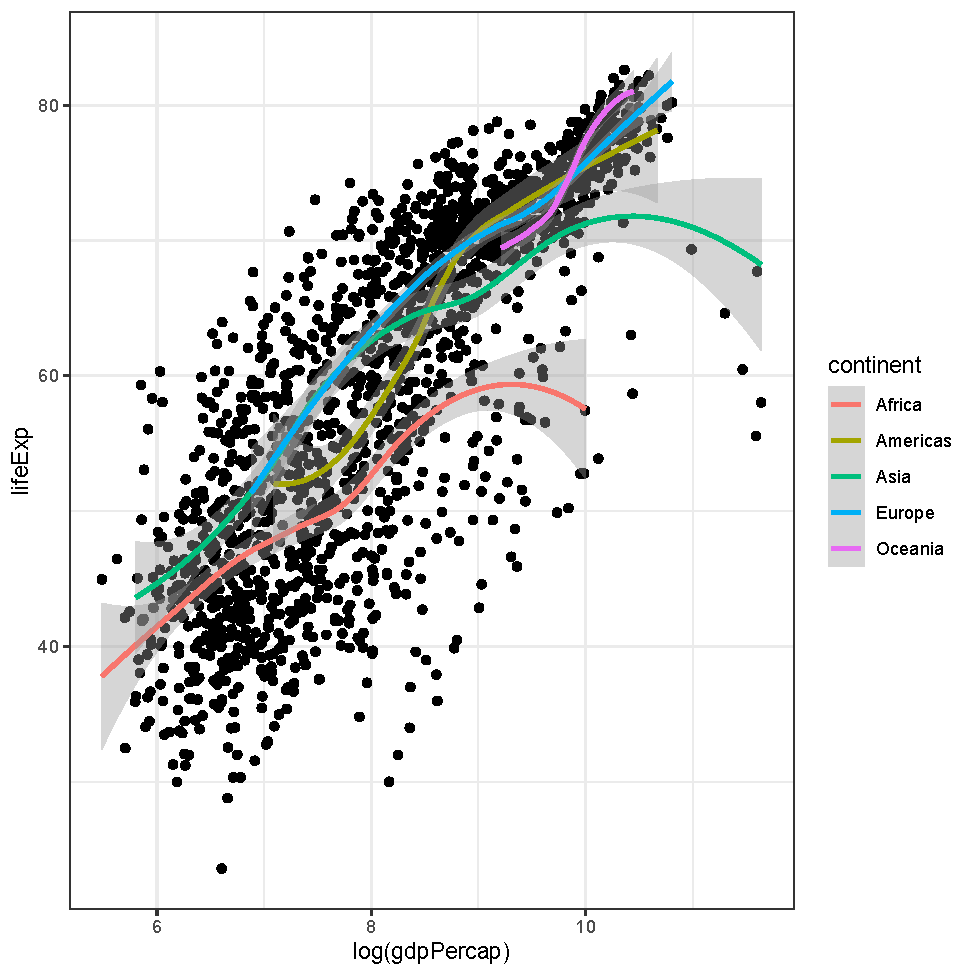
\includegraphics[width=0.7\linewidth,keepaspectratio]{Multivariable_Data_Analysis_files/figure-latex/unnamed-chunk-41-1} \end{center}

This is the classic theme

\begin{Shaded}
\begin{Highlighting}[]
\NormalTok{mypop }\SpecialCharTok{+} \FunctionTok{theme\_classic}\NormalTok{()}
\end{Highlighting}
\end{Shaded}

\begin{center}\includegraphics[width=0.7\linewidth,keepaspectratio]{Multivariable_Data_Analysis_files/figure-latex/unnamed-chunk-42-1} \end{center}

\hypertarget{saving-plot}{%
\section{Saving plot}\label{saving-plot}}

In R, you can save the plot into different format. You can also set other parameters such as the dpi and the size for the plot. One of the preferred formats for saving a plot is as a PDF format.

\hypertarget{saving-plot-using-ggplot2}{%
\section{Saving plot using ggplot2}\label{saving-plot-using-ggplot2}}

Here, we will show how to save plots in R. In this example, let us use the object for the plot named \texttt{mypop} and add a title, an x label, an y label and choose the classic theme,

\begin{Shaded}
\begin{Highlighting}[]
\NormalTok{myplot }\OtherTok{\textless{}{-}}\NormalTok{ mypop }\SpecialCharTok{+} 
\FunctionTok{ggtitle}\NormalTok{(}\StringTok{"Scatterplot showing the relationship of GDP in log and life expectancy:}
\StringTok{                }\SpecialCharTok{\textbackslash{}n}\StringTok{Data from Gapminder"}\NormalTok{) }\SpecialCharTok{+} \FunctionTok{ylab}\NormalTok{(}\StringTok{"Life Expentancy"}\NormalTok{) }\SpecialCharTok{+} 
  \FunctionTok{xlab}\NormalTok{(}\StringTok{"Percapita GDP in log"}\NormalTok{) }\SpecialCharTok{+}
  \FunctionTok{scale\_x\_continuous}\NormalTok{(}\AttributeTok{breaks =} \FunctionTok{seq}\NormalTok{(}\DecValTok{0}\NormalTok{,}\DecValTok{12}\NormalTok{,}\DecValTok{1}\NormalTok{)) }\SpecialCharTok{+}
  \FunctionTok{theme\_classic}\NormalTok{()}
\NormalTok{myplot}
\end{Highlighting}
\end{Shaded}

\begin{center}\includegraphics[width=0.7\linewidth,keepaspectratio]{Multivariable_Data_Analysis_files/figure-latex/unnamed-chunk-43-1} \end{center}

We now can see a nice plot. And next, we want to save the plot (currently on the screen) to these formats:

\begin{enumerate}
\def\labelenumi{\arabic{enumi}.}
\tightlist
\item
  \texttt{pdf} format
\item
  \texttt{png} format
\item
  \texttt{jpg} format
\end{enumerate}

The codes we can use are:

\begin{Shaded}
\begin{Highlighting}[]
\FunctionTok{library}\NormalTok{(here)}
\FunctionTok{ggsave}\NormalTok{(}\AttributeTok{plot =}\NormalTok{ myplot, }\FunctionTok{here}\NormalTok{(}\StringTok{"plots"}\NormalTok{,}\StringTok{"my\_pdf\_plot.pdf"}\NormalTok{))}
\FunctionTok{ggsave}\NormalTok{(}\AttributeTok{plot =}\NormalTok{ myplot, }\FunctionTok{here}\NormalTok{(}\StringTok{"plots"}\NormalTok{,}\StringTok{"my\_png\_plot.png"}\NormalTok{)) }
\FunctionTok{ggsave}\NormalTok{(}\AttributeTok{plot =}\NormalTok{ myplot, }\FunctionTok{here}\NormalTok{(}\StringTok{"plots"}\NormalTok{,}\StringTok{"my\_jpg\_plot.jpg"}\NormalTok{))}
\end{Highlighting}
\end{Shaded}

If we want to add more customization before saving the plot, for example, we want to set these parameters:

\begin{enumerate}
\def\labelenumi{\arabic{enumi}.}
\tightlist
\item
  width = 10 cm (or you can use \texttt{in})
\item
  height = 6 cm (or you can use \texttt{in})
\item
  dpi = 150. dpi is dots per inch
\end{enumerate}

Now, you can run these codes

\begin{Shaded}
\begin{Highlighting}[]
\FunctionTok{ggsave}\NormalTok{(}\AttributeTok{plot =}\NormalTok{ myplot, }\FunctionTok{here}\NormalTok{(}\StringTok{\textquotesingle{}plots\textquotesingle{}}\NormalTok{,}\StringTok{\textquotesingle{}my\_pdf\_plot2.pdf\textquotesingle{}}\NormalTok{), }
                           \AttributeTok{width =} \DecValTok{10}\NormalTok{, }\AttributeTok{height =} \DecValTok{6}\NormalTok{, }\AttributeTok{units =} \StringTok{"in"}\NormalTok{,}
                           \AttributeTok{dpi =} \DecValTok{150}\NormalTok{, }\AttributeTok{device =} \StringTok{\textquotesingle{}pdf\textquotesingle{}}\NormalTok{)}
\FunctionTok{ggsave}\NormalTok{(}\AttributeTok{plot =}\NormalTok{ myplot, }\FunctionTok{here}\NormalTok{(}\StringTok{\textquotesingle{}plots\textquotesingle{}}\NormalTok{,}\StringTok{\textquotesingle{}my\_png\_plot2.png\textquotesingle{}}\NormalTok{), }
       \AttributeTok{width =} \DecValTok{10}\NormalTok{, }\AttributeTok{height =} \DecValTok{6}\NormalTok{, }\AttributeTok{units =} \StringTok{"cm"}\NormalTok{, }
       \AttributeTok{dpi =} \DecValTok{150}\NormalTok{, }\AttributeTok{device =} \StringTok{\textquotesingle{}png\textquotesingle{}}\NormalTok{)}
\FunctionTok{ggsave}\NormalTok{(}\AttributeTok{plot =}\NormalTok{ myplot, }\FunctionTok{here}\NormalTok{(}\StringTok{"plots"}\NormalTok{,}\StringTok{"my\_jpg\_plot2.jpg"}\NormalTok{), }
       \AttributeTok{width =} \DecValTok{10}\NormalTok{, }\AttributeTok{height =} \DecValTok{6}\NormalTok{, }\AttributeTok{units =} \StringTok{"cm"}\NormalTok{,}
       \AttributeTok{dpi =} \DecValTok{150}\NormalTok{, }\AttributeTok{device =} \StringTok{\textquotesingle{}jpg\textquotesingle{}}\NormalTok{)}
\end{Highlighting}
\end{Shaded}

\hypertarget{data-wrangling}{%
\chapter{Data Wrangling}\label{data-wrangling}}

\hypertarget{definition-of-data-wrangling}{%
\section{Definition of data wrangling}\label{definition-of-data-wrangling}}

Data wrangling is also known as Data Munging or Data Transformation. It is loosely the process of manually converting or mapping data from one ``raw'' form into another format. The process allows for more convenient consumption of the data. In doing so, we will be using semi-automated tools in RStudio. You can find more information here \url{https://community.modeanalytics.com/sql/tutorial/data-wrangling-with-sql/}

\hypertarget{data-wrangling-with-dplyr-package}{%
\section{\texorpdfstring{Data wrangling with \textbf{dplyr} package}{Data wrangling with dplyr package}}\label{data-wrangling-with-dplyr-package}}

\hypertarget{dplyr-package}{%
\subsection{\texorpdfstring{\textbf{dplyr} package}{dplyr package}}\label{dplyr-package}}

\textbf{dplyr} is a package grouped inside \textbf{tidyverse} collection of packages. \textbf{dplyr} package is a very useful package to munge or wrangle or to tranform your data. It is a grammar of data manipulation. It provides a consistent set of verbs that help you solve the most common data manipulation challenges. This \textbf{tidyverse} webpage \url{https://github.com/tidyverse/dplyr} has more information and examples.

\hypertarget{common-procedures-for-doing-data-transformation}{%
\section{Common procedures for doing data transformation}\label{common-procedures-for-doing-data-transformation}}

The common data wrangling procedures that data analyst does include:

\begin{enumerate}
\def\labelenumi{\arabic{enumi}.}
\tightlist
\item
  reducing the size of dataset by selecting certain variables (or columns)
\item
  generating new variable from existing variables
\item
  sorting observation of a variable
\item
  grouping observations based on certain criteria
\item
  reducing variable to groups to in order to estimate summary statistic
\end{enumerate}

\hypertarget{some-dplyr-functions}{%
\section{\texorpdfstring{Some \textbf{dplyr} functions}{Some dplyr functions}}\label{some-dplyr-functions}}

For the procedures listed above, the corresponding \textbf{dplyr} functions are

\begin{enumerate}
\def\labelenumi{\arabic{enumi}.}
\tightlist
\item
  \texttt{dplyr::select()} - to select a number of variables from a dataframe
\item
  \texttt{dplyr::mutate()} - to generate a new variable from existing variables
\item
  \texttt{dplyr::arrange()} - to sort observation of a variable
\item
  \texttt{dplyr::filter()} - to group observations that fulfil certain criteria
\item
  \texttt{dplyr::group\_by()} and \texttt{dplyr::summarize()} - to reduce variable to groups in order to provide summary statistic
\end{enumerate}

\hypertarget{create-a-new-project-or-set-your-working-directory}{%
\section{Create a new project or set your working directory}\label{create-a-new-project-or-set-your-working-directory}}

It is very important to ensure you know where your working directory is. To do so, the best practice is \emph{is to create a new project everytime you want to start new analysis with R}. To do so, create a new project by \texttt{File\ -\textgreater{}\ New\ Project}. If you do not start with a new project, you still need to know \textbf{Where is my working directory?}.

So, again we emphasize that every time you want to start processing your data, please make sure:

\begin{enumerate}
\def\labelenumi{\arabic{enumi}.}
\tightlist
\item
  you use R project. It is much easier and cleaner to start your work with a new R project. Once you have done or need to log off your computer, close the project and reopen the project the next time you need to.\\
\item
  that if you are not using R project, you are inside the correct working directory. Type \texttt{getwd()} to display the active \textbf{working directory}. And to set a new working directory use the function \texttt{setwd()}. Once you are know where your working directory is, you can start read or import data into your working directory.
\end{enumerate}

Once you are inside the project, you can import your data if necessary. Remember, there are a number of packages you can use to read the data into R. R can read almost all (if not all format) types of data format. For example, we know that common data format are the:

\begin{enumerate}
\def\labelenumi{\arabic{enumi}.}
\tightlist
\item
  SPSS (\texttt{.sav}) format,
\item
  Stata (\texttt{.dta}) format,
\item
  SAS format,
\item
  MS Excel (\texttt{.xlsx}) format
\item
  Comma-separated-values \texttt{.csv} format.
\end{enumerate}

But they are other formats too for examples data in DICOM format. DICOM format data includes data from CT scan and MRI images. There are data in shapefile format to store geographical information. Three packages - \textbf{haven}, \textbf{readr} and \textbf{foreign} packages - are very useful to read or import your data into R memory.

\begin{enumerate}
\def\labelenumi{\arabic{enumi}.}
\tightlist
\item
  \textbf{readr} provides a fast and friendly way to read rectangular data (like csv, tsv, and fwf).
\item
  \textbf{readxl} reads .xls and .xlsx sheets.
\item
  \textbf{haven} reads SPSS, Stata, and SAS data.
\end{enumerate}

\hypertarget{starwars-data}{%
\section{\texorpdfstring{\emph{starwars} data}{starwars data}}\label{starwars-data}}

To make life easier and to facilitate reproducibility, we will use examples available from the public domains. We will produce and reproduce the outputs demonstrated on \textbf{tidyverse} website (\url{https://github.com/tidyverse/dplyr}). One of the useful datasets is \texttt{starwars} dataset. The \texttt{starwars} data comes together with \textbf{dplyr} package. This original source of data is from SWAPI, the Star Wars API accessible at \url{http://swapi.co/}.

The \texttt{starwars} data is class of \texttt{tibble}. The data have:

\begin{itemize}
\tightlist
\item
  87 rows (observations)
\item
  13 columns (variables)
\end{itemize}

Now, let us:

\begin{enumerate}
\def\labelenumi{\arabic{enumi}.}
\tightlist
\item
  load the \textbf{tidyverse} package
\item
  examine the column names (variable names)
\end{enumerate}

Loading \textbf{tidyverse} packages will load \textbf{dplyr} automatically. If you want to load only \textbf{dplyr}, just type \texttt{library(dplyr)}.

\begin{Shaded}
\begin{Highlighting}[]
\FunctionTok{library}\NormalTok{(dplyr)}
\end{Highlighting}
\end{Shaded}

Take a peek at the \texttt{starwars} data

\begin{Shaded}
\begin{Highlighting}[]
\FunctionTok{glimpse}\NormalTok{(starwars)}
\end{Highlighting}
\end{Shaded}

\begin{verbatim}
## Rows: 87
## Columns: 14
## $ name       <chr> "Luke Skywalker", "C-3PO", "R2-D2", "Darth Vader", "Leia Or~
## $ height     <int> 172, 167, 96, 202, 150, 178, 165, 97, 183, 182, 188, 180, 2~
## $ mass       <dbl> 77.0, 75.0, 32.0, 136.0, 49.0, 120.0, 75.0, 32.0, 84.0, 77.~
## $ hair_color <chr> "blond", NA, NA, "none", "brown", "brown, grey", "brown", N~
## $ skin_color <chr> "fair", "gold", "white, blue", "white", "light", "light", "~
## $ eye_color  <chr> "blue", "yellow", "red", "yellow", "brown", "blue", "blue",~
## $ birth_year <dbl> 19.0, 112.0, 33.0, 41.9, 19.0, 52.0, 47.0, NA, 24.0, 57.0, ~
## $ sex        <chr> "male", "none", "none", "male", "female", "male", "female",~
## $ gender     <chr> "masculine", "masculine", "masculine", "masculine", "femini~
## $ homeworld  <chr> "Tatooine", "Tatooine", "Naboo", "Tatooine", "Alderaan", "T~
## $ species    <chr> "Human", "Droid", "Droid", "Human", "Human", "Human", "Huma~
## $ films      <list> <"The Empire Strikes Back", "Revenge of the Sith", "Return~
## $ vehicles   <list> <"Snowspeeder", "Imperial Speeder Bike">, <>, <>, <>, "Imp~
## $ starships  <list> <"X-wing", "Imperial shuttle">, <>, <>, "TIE Advanced x1",~
\end{verbatim}

Next, we examine the first 10 observations of the data. There are 77 more rows NOT SHOWN. You can also see the types of the variables:

\begin{enumerate}
\def\labelenumi{\arabic{enumi}.}
\tightlist
\item
  \texttt{chr} (character),
\item
  \texttt{int} (integer),
\item
  \texttt{dbl} (double)
\end{enumerate}

\begin{Shaded}
\begin{Highlighting}[]
\NormalTok{starwars}
\end{Highlighting}
\end{Shaded}

\begin{verbatim}
## # A tibble: 87 x 14
##    name    height  mass hair_color  skin_color eye_color birth_year sex   gender
##    <chr>    <int> <dbl> <chr>       <chr>      <chr>          <dbl> <chr> <chr> 
##  1 Luke S~    172    77 blond       fair       blue            19   male  mascu~
##  2 C-3PO      167    75 <NA>        gold       yellow         112   none  mascu~
##  3 R2-D2       96    32 <NA>        white, bl~ red             33   none  mascu~
##  4 Darth ~    202   136 none        white      yellow          41.9 male  mascu~
##  5 Leia O~    150    49 brown       light      brown           19   fema~ femin~
##  6 Owen L~    178   120 brown, grey light      blue            52   male  mascu~
##  7 Beru W~    165    75 brown       light      blue            47   fema~ femin~
##  8 R5-D4       97    32 <NA>        white, red red             NA   none  mascu~
##  9 Biggs ~    183    84 black       light      brown           24   male  mascu~
## 10 Obi-Wa~    182    77 auburn, wh~ fair       blue-gray       57   male  mascu~
## # ... with 77 more rows, and 5 more variables: homeworld <chr>, species <chr>,
## #   films <list>, vehicles <list>, starships <list>
\end{verbatim}

\hypertarget{select-variables-generate-new-variable-and-rename-variable}{%
\section{Select variables, generate new variable and rename variable}\label{select-variables-generate-new-variable-and-rename-variable}}

We will work with these functions

\begin{itemize}
\tightlist
\item
  \texttt{dplyr::select()}
\item
  \texttt{dplyr::mutate()} and
\item
  \texttt{dplyr::rename()}
\end{itemize}

\hypertarget{select-variables-using-dplyrselect}{%
\subsection{\texorpdfstring{Select variables using \texttt{dplyr::select()}}{Select variables using dplyr::select()}}\label{select-variables-using-dplyrselect}}

When you work with large datasets with many columns, sometimes it is easier to select only the necessary columns to reduce the size of dataset. This is possible by creating a smaller dataset (less variables). Then you can work on at the initial part of data analysis with this smaller dataset. This will greatly help data exploration.

To create smaller datasets, select some of the columns (variables) in the dataset. For example, in \texttt{starwars} data, we have 13 variables. From this dataset, let us generate a new dataset named as \texttt{mysw} with only these 4 variables ,
1. name
2. height
3. mass
4. gender

\begin{Shaded}
\begin{Highlighting}[]
\NormalTok{mysw }\OtherTok{\textless{}{-}}\NormalTok{ starwars }\SpecialCharTok{\%\textgreater{}\%} \FunctionTok{select}\NormalTok{(name, gender, height, mass)}
\NormalTok{mysw}
\end{Highlighting}
\end{Shaded}

\begin{verbatim}
## # A tibble: 87 x 4
##    name               gender    height  mass
##    <chr>              <chr>      <int> <dbl>
##  1 Luke Skywalker     masculine    172    77
##  2 C-3PO              masculine    167    75
##  3 R2-D2              masculine     96    32
##  4 Darth Vader        masculine    202   136
##  5 Leia Organa        feminine     150    49
##  6 Owen Lars          masculine    178   120
##  7 Beru Whitesun lars feminine     165    75
##  8 R5-D4              masculine     97    32
##  9 Biggs Darklighter  masculine    183    84
## 10 Obi-Wan Kenobi     masculine    182    77
## # ... with 77 more rows
\end{verbatim}

The new dataset \texttt{mysw} is now created. You can see it in the \texttt{Environment} pane.

\hypertarget{generate-varibale-using-dplyrmutate}{%
\subsection{\texorpdfstring{Generate varibale using \texttt{dplyr::mutate()}}{Generate varibale using dplyr::mutate()}}\label{generate-varibale-using-dplyrmutate}}

With \texttt{dplyr::mutate()}, you can generate new variable. For example, in the dataset \texttt{mysw}, we want to create a new variable named as \texttt{bmi}. This variable equals mass in kg divided by squared height (in meter)

\[bmi = \frac{kg}{m^2}\]

\begin{Shaded}
\begin{Highlighting}[]
\NormalTok{mysw }\OtherTok{\textless{}{-}}\NormalTok{ mysw }\SpecialCharTok{\%\textgreater{}\%} \FunctionTok{mutate}\NormalTok{(}\AttributeTok{bmi =}\NormalTok{ mass}\SpecialCharTok{/}\NormalTok{(height}\SpecialCharTok{/}\DecValTok{100}\NormalTok{)}\SpecialCharTok{\^{}}\DecValTok{2}\NormalTok{)}
\NormalTok{mysw}
\end{Highlighting}
\end{Shaded}

\begin{verbatim}
## # A tibble: 87 x 5
##    name               gender    height  mass   bmi
##    <chr>              <chr>      <int> <dbl> <dbl>
##  1 Luke Skywalker     masculine    172    77  26.0
##  2 C-3PO              masculine    167    75  26.9
##  3 R2-D2              masculine     96    32  34.7
##  4 Darth Vader        masculine    202   136  33.3
##  5 Leia Organa        feminine     150    49  21.8
##  6 Owen Lars          masculine    178   120  37.9
##  7 Beru Whitesun lars feminine     165    75  27.5
##  8 R5-D4              masculine     97    32  34.0
##  9 Biggs Darklighter  masculine    183    84  25.1
## 10 Obi-Wan Kenobi     masculine    182    77  23.2
## # ... with 77 more rows
\end{verbatim}

Now, your dataset \texttt{mysw} has 5 columns (variables). The last variable is \texttt{bmi}

\hypertarget{rename-variable-using-dplyrrename}{%
\subsection{\texorpdfstring{Rename variable using \texttt{dplyr::rename()}}{Rename variable using dplyr::rename()}}\label{rename-variable-using-dplyrrename}}

Now,

\begin{enumerate}
\def\labelenumi{\arabic{enumi}.}
\tightlist
\item
  create a new variable \emph{bmi2} which equals \(bmi^2\).
\item
  rename \emph{bmi2} to \emph{bmisq}
\end{enumerate}

\begin{Shaded}
\begin{Highlighting}[]
\NormalTok{mysw }\OtherTok{\textless{}{-}}\NormalTok{ mysw }\SpecialCharTok{\%\textgreater{}\%} \FunctionTok{mutate}\NormalTok{(}\AttributeTok{bmi2 =}\NormalTok{ bmi}\SpecialCharTok{\^{}}\DecValTok{2}\NormalTok{)}
\NormalTok{mysw}
\end{Highlighting}
\end{Shaded}

\begin{verbatim}
## # A tibble: 87 x 6
##    name               gender    height  mass   bmi  bmi2
##    <chr>              <chr>      <int> <dbl> <dbl> <dbl>
##  1 Luke Skywalker     masculine    172    77  26.0  677.
##  2 C-3PO              masculine    167    75  26.9  723.
##  3 R2-D2              masculine     96    32  34.7 1206.
##  4 Darth Vader        masculine    202   136  33.3 1111.
##  5 Leia Organa        feminine     150    49  21.8  474.
##  6 Owen Lars          masculine    178   120  37.9 1434.
##  7 Beru Whitesun lars feminine     165    75  27.5  759.
##  8 R5-D4              masculine     97    32  34.0 1157.
##  9 Biggs Darklighter  masculine    183    84  25.1  629.
## 10 Obi-Wan Kenobi     masculine    182    77  23.2  540.
## # ... with 77 more rows
\end{verbatim}

\begin{Shaded}
\begin{Highlighting}[]
\NormalTok{mysw }\OtherTok{\textless{}{-}}\NormalTok{ mysw }\SpecialCharTok{\%\textgreater{}\%} \FunctionTok{rename}\NormalTok{(}\AttributeTok{bmisq =}\NormalTok{ bmi2)}
\NormalTok{mysw}
\end{Highlighting}
\end{Shaded}

\begin{verbatim}
## # A tibble: 87 x 6
##    name               gender    height  mass   bmi bmisq
##    <chr>              <chr>      <int> <dbl> <dbl> <dbl>
##  1 Luke Skywalker     masculine    172    77  26.0  677.
##  2 C-3PO              masculine    167    75  26.9  723.
##  3 R2-D2              masculine     96    32  34.7 1206.
##  4 Darth Vader        masculine    202   136  33.3 1111.
##  5 Leia Organa        feminine     150    49  21.8  474.
##  6 Owen Lars          masculine    178   120  37.9 1434.
##  7 Beru Whitesun lars feminine     165    75  27.5  759.
##  8 R5-D4              masculine     97    32  34.0 1157.
##  9 Biggs Darklighter  masculine    183    84  25.1  629.
## 10 Obi-Wan Kenobi     masculine    182    77  23.2  540.
## # ... with 77 more rows
\end{verbatim}

\hypertarget{sorting-data-and-select-observation}{%
\section{Sorting data and select observation}\label{sorting-data-and-select-observation}}

The function \texttt{dplyr::arrange()} can sort the data. And the function \texttt{dplyr::filter()} allows you to select observations based on your criteria.

\hypertarget{sorting-data-using-dplyrarrange}{%
\subsection{\texorpdfstring{Sorting data using \texttt{dplyr::arrange()}}{Sorting data using dplyr::arrange()}}\label{sorting-data-using-dplyrarrange}}

We can sort data in ascending or descending order. To do that, we will use \texttt{dplyr::arrange()}. It will sort the observation based on the values of the specified variable. For dataset \texttt{mysw}, let us sort the \texttt{bmi} from the biggest bmi (descending).

\begin{Shaded}
\begin{Highlighting}[]
\NormalTok{mysw }\OtherTok{\textless{}{-}}\NormalTok{ mysw }\SpecialCharTok{\%\textgreater{}\%} \FunctionTok{arrange}\NormalTok{(}\FunctionTok{desc}\NormalTok{(bmi))}
\NormalTok{mysw}
\end{Highlighting}
\end{Shaded}

\begin{verbatim}
## # A tibble: 87 x 6
##    name                  gender    height  mass   bmi   bmisq
##    <chr>                 <chr>      <int> <dbl> <dbl>   <dbl>
##  1 Jabba Desilijic Tiure masculine    175  1358 443.  196629.
##  2 Dud Bolt              masculine     94    45  50.9   2594.
##  3 Yoda                  masculine     66    17  39.0   1523.
##  4 Owen Lars             masculine    178   120  37.9   1434.
##  5 IG-88                 masculine    200   140  35     1225 
##  6 R2-D2                 masculine     96    32  34.7   1206.
##  7 Grievous              masculine    216   159  34.1   1161.
##  8 R5-D4                 masculine     97    32  34.0   1157.
##  9 Jek Tono Porkins      masculine    180   110  34.0   1153.
## 10 Darth Vader           masculine    202   136  33.3   1111.
## # ... with 77 more rows
\end{verbatim}

Now, we will replace the dataset \texttt{mysw} with data that contain the \texttt{bmi} values from the lowest to the biggest bmi (ascending).

\begin{Shaded}
\begin{Highlighting}[]
\NormalTok{mysw }\OtherTok{\textless{}{-}}\NormalTok{ mysw }\SpecialCharTok{\%\textgreater{}\%} \FunctionTok{arrange}\NormalTok{(bmi)}
\NormalTok{mysw}
\end{Highlighting}
\end{Shaded}

\begin{verbatim}
## # A tibble: 87 x 6
##    name          gender    height  mass   bmi bmisq
##    <chr>         <chr>      <int> <dbl> <dbl> <dbl>
##  1 Wat Tambor    masculine    193    48  12.9  166.
##  2 Adi Gallia    feminine     184    50  14.8  218.
##  3 Sly Moore     <NA>         178    48  15.1  230.
##  4 Roos Tarpals  masculine    224    82  16.3  267.
##  5 Padmé Amidala feminine     165    45  16.5  273.
##  6 Lama Su       masculine    229    88  16.8  282.
##  7 Jar Jar Binks masculine    196    66  17.2  295.
##  8 Ayla Secura   feminine     178    55  17.4  301.
##  9 Shaak Ti      feminine     178    57  18.0  324.
## 10 Barriss Offee feminine     166    50  18.1  329.
## # ... with 77 more rows
\end{verbatim}

\hypertarget{select-observation-using-dplyrfilter}{%
\subsection{\texorpdfstring{Select observation using \texttt{dplyr::filter()}}{Select observation using dplyr::filter()}}\label{select-observation-using-dplyrfilter}}

To select observations based on certain criteria, we use the \texttt{dplyr::filter()} function. Here, in this example, we will create a new dataset (which we will name as \texttt{mysw\_m\_40}) that contains observations with these criteria:

\begin{itemize}
\tightlist
\item
  gender is male AND
\item
  bmi at or above 40
\end{itemize}

\begin{Shaded}
\begin{Highlighting}[]
\NormalTok{mysw\_m\_40 }\OtherTok{\textless{}{-}}\NormalTok{ mysw }\SpecialCharTok{\%\textgreater{}\%} \FunctionTok{filter}\NormalTok{(gender }\SpecialCharTok{==} \StringTok{\textquotesingle{}male\textquotesingle{}}\NormalTok{, bmi }\SpecialCharTok{\textgreater{}=} \DecValTok{40}\NormalTok{)}
\NormalTok{mysw\_m\_40}
\end{Highlighting}
\end{Shaded}

\begin{verbatim}
## # A tibble: 0 x 6
## # ... with 6 variables: name <chr>, gender <chr>, height <int>, mass <dbl>,
## #   bmi <dbl>, bmisq <dbl>
\end{verbatim}

Next, we will create a new dataset (named as \texttt{mysw\_ht\_45}) that contain

\begin{itemize}
\tightlist
\item
  \texttt{height} above 200 OR \texttt{BMI} above 45, AND
\item
  does not include \texttt{NA} (which is missing value) observation for \texttt{bmi}
\end{itemize}

\begin{Shaded}
\begin{Highlighting}[]
\NormalTok{mysw\_ht\_45 }\OtherTok{\textless{}{-}}\NormalTok{ mysw }\SpecialCharTok{\%\textgreater{}\%} \FunctionTok{filter}\NormalTok{(height }\SpecialCharTok{\textgreater{}}\DecValTok{200} \SpecialCharTok{|}\NormalTok{ bmi }\SpecialCharTok{\textgreater{}}\DecValTok{45}\NormalTok{, bmi }\SpecialCharTok{!=} \StringTok{\textquotesingle{}NA\textquotesingle{}}\NormalTok{)}
\NormalTok{mysw\_ht\_45}
\end{Highlighting}
\end{Shaded}

\begin{verbatim}
## # A tibble: 9 x 6
##   name                  gender    height  mass   bmi   bmisq
##   <chr>                 <chr>      <int> <dbl> <dbl>   <dbl>
## 1 Roos Tarpals          masculine    224    82  16.3    267.
## 2 Lama Su               masculine    229    88  16.8    282.
## 3 Tion Medon            masculine    206    80  18.9    355.
## 4 Chewbacca             masculine    228   112  21.5    464.
## 5 Tarfful               masculine    234   136  24.8    617.
## 6 Darth Vader           masculine    202   136  33.3   1111.
## 7 Grievous              masculine    216   159  34.1   1161.
## 8 Dud Bolt              masculine     94    45  50.9   2594.
## 9 Jabba Desilijic Tiure masculine    175  1358 443.  196629.
\end{verbatim}

\hypertarget{group-data-and-get-summary-statistics}{%
\section{Group data and get summary statistics}\label{group-data-and-get-summary-statistics}}

The\texttt{dplyr::group\_by()} function allows us to group data based on categorical variable. Using the \texttt{dplyr::summarize} we do summary statistics for the overall data or for groups created using \texttt{group\_by()} function.

\hypertarget{group-data-using-dplyrgroup_by}{%
\subsection{\texorpdfstring{Group data using \texttt{dplyr::group\_by()}}{Group data using dplyr::group\_by()}}\label{group-data-using-dplyrgroup_by}}

The \texttt{group\_by} function will prepare the data for group analysis. For example,

\begin{enumerate}
\def\labelenumi{\arabic{enumi}.}
\tightlist
\item
  to get summary values for mean \texttt{bmi}, mean \texttt{ht} and mean \texttt{mass}
\item
  for male, female, hermaphrodite and none (\texttt{gender} variable)
\end{enumerate}

\begin{Shaded}
\begin{Highlighting}[]
\NormalTok{mysw\_g }\OtherTok{\textless{}{-}}\NormalTok{ mysw }\SpecialCharTok{\%\textgreater{}\%} \FunctionTok{group\_by}\NormalTok{(gender)}
\NormalTok{mysw\_g}
\end{Highlighting}
\end{Shaded}

\begin{verbatim}
## # A tibble: 87 x 6
## # Groups:   gender [3]
##    name          gender    height  mass   bmi bmisq
##    <chr>         <chr>      <int> <dbl> <dbl> <dbl>
##  1 Wat Tambor    masculine    193    48  12.9  166.
##  2 Adi Gallia    feminine     184    50  14.8  218.
##  3 Sly Moore     <NA>         178    48  15.1  230.
##  4 Roos Tarpals  masculine    224    82  16.3  267.
##  5 Padmé Amidala feminine     165    45  16.5  273.
##  6 Lama Su       masculine    229    88  16.8  282.
##  7 Jar Jar Binks masculine    196    66  17.2  295.
##  8 Ayla Secura   feminine     178    55  17.4  301.
##  9 Shaak Ti      feminine     178    57  18.0  324.
## 10 Barriss Offee feminine     166    50  18.1  329.
## # ... with 77 more rows
\end{verbatim}

\hypertarget{summary-statistic-using-dplyrsummarize}{%
\subsection{\texorpdfstring{Summary statistic using \texttt{dplyr::summarize()}}{Summary statistic using dplyr::summarize()}}\label{summary-statistic-using-dplyrsummarize}}

Now that we have a group data named \texttt{mysw\_g}, now, we would summarize our data using the mean and standard deviation (SD) for the groups specified above.

\begin{Shaded}
\begin{Highlighting}[]
\NormalTok{mysw\_g }\SpecialCharTok{\%\textgreater{}\%} \FunctionTok{summarise}\NormalTok{(}\AttributeTok{meanbmi =} \FunctionTok{mean}\NormalTok{(bmi, }\AttributeTok{na.rm =} \ConstantTok{TRUE}\NormalTok{), }
                     \AttributeTok{meanht  =} \FunctionTok{mean}\NormalTok{(height, }\AttributeTok{na.rm =} \ConstantTok{TRUE}\NormalTok{),}
                     \AttributeTok{meanmass =} \FunctionTok{mean}\NormalTok{(mass, }\AttributeTok{na.rm =} \ConstantTok{TRUE}\NormalTok{),}
                     \AttributeTok{sdbmi =} \FunctionTok{sd}\NormalTok{(bmi, }\AttributeTok{na.rm =} \ConstantTok{TRUE}\NormalTok{),}
                     \AttributeTok{sdht =} \FunctionTok{sd}\NormalTok{(height, }\AttributeTok{na.rm =} \ConstantTok{TRUE}\NormalTok{),}
                     \AttributeTok{sdmass =} \FunctionTok{sd}\NormalTok{(mass, }\AttributeTok{na.rm =} \ConstantTok{TRUE}\NormalTok{))}
\end{Highlighting}
\end{Shaded}

\begin{verbatim}
## # A tibble: 3 x 7
##   gender    meanbmi meanht meanmass sdbmi  sdht sdmass
##   <chr>       <dbl>  <dbl>    <dbl> <dbl> <dbl>  <dbl>
## 1 feminine     19.2   165.     54.7  3.69 23.6    8.59
## 2 masculine    34.7   177.    106.  60.0  37.6  185.  
## 3 <NA>         15.1   181.     48   NA     2.89  NA
\end{verbatim}

To calculate the frequencies for one variable

\begin{Shaded}
\begin{Highlighting}[]
\NormalTok{freq\_species }\OtherTok{\textless{}{-}}\NormalTok{ starwars }\SpecialCharTok{\%\textgreater{}\%} \FunctionTok{count}\NormalTok{(species, }\AttributeTok{sort =} \ConstantTok{TRUE}\NormalTok{)}
\NormalTok{freq\_species}
\end{Highlighting}
\end{Shaded}

\begin{verbatim}
## # A tibble: 38 x 2
##    species      n
##    <chr>    <int>
##  1 Human       35
##  2 Droid        6
##  3 <NA>         4
##  4 Gungan       3
##  5 Kaminoan     2
##  6 Mirialan     2
##  7 Twi'lek      2
##  8 Wookiee      2
##  9 Zabrak       2
## 10 Aleena       1
## # ... with 28 more rows
\end{verbatim}

And to calculate the frequencies for two variables. You can add the categorical or factor variable to get the frequencies for more groups.

\begin{Shaded}
\begin{Highlighting}[]
\NormalTok{freq\_species\_home }\OtherTok{\textless{}{-}}\NormalTok{ starwars }\SpecialCharTok{\%\textgreater{}\%} \FunctionTok{count}\NormalTok{(species, homeworld, }\AttributeTok{sort =} \ConstantTok{TRUE}\NormalTok{)}
\NormalTok{freq\_species\_home}
\end{Highlighting}
\end{Shaded}

\begin{verbatim}
## # A tibble: 58 x 3
##    species  homeworld     n
##    <chr>    <chr>     <int>
##  1 Human    Tatooine      8
##  2 Human    Naboo         5
##  3 Human    <NA>          5
##  4 Droid    <NA>          3
##  5 Gungan   Naboo         3
##  6 Human    Alderaan      3
##  7 Droid    Tatooine      2
##  8 Human    Corellia      2
##  9 Human    Coruscant     2
## 10 Kaminoan Kamino        2
## # ... with 48 more rows
\end{verbatim}

\hypertarget{more-complicated-dplyr-verbs}{%
\section{\texorpdfstring{More complicated \textbf{dplyr} verbs}{More complicated dplyr verbs}}\label{more-complicated-dplyr-verbs}}

To be more efficent, use multiple \textbf{dplyr} functions in one line of R code. For example,

\begin{Shaded}
\begin{Highlighting}[]
\NormalTok{starwars }\SpecialCharTok{\%\textgreater{}\%} \FunctionTok{filter}\NormalTok{(gender }\SpecialCharTok{==} \StringTok{"male"}\NormalTok{, height }\SpecialCharTok{\textgreater{}} \DecValTok{100}\NormalTok{, mass }\SpecialCharTok{\textgreater{}} \DecValTok{100}\NormalTok{) }\SpecialCharTok{\%\textgreater{}\%} 
  \FunctionTok{select}\NormalTok{(height, mass, species) }\SpecialCharTok{\%\textgreater{}\%}
  \FunctionTok{group\_by}\NormalTok{(species) }\SpecialCharTok{\%\textgreater{}\%}
  \FunctionTok{summarize}\NormalTok{(}\AttributeTok{mean\_ht =} \FunctionTok{mean}\NormalTok{(height, }\AttributeTok{na.rm =} \ConstantTok{TRUE}\NormalTok{), }
            \AttributeTok{mean\_mass =} \FunctionTok{mean}\NormalTok{(mass, }\AttributeTok{na.rm =} \ConstantTok{TRUE}\NormalTok{),}
            \AttributeTok{freq =} \FunctionTok{n}\NormalTok{())}
\end{Highlighting}
\end{Shaded}

\begin{verbatim}
## # A tibble: 0 x 4
## # ... with 4 variables: species <chr>, mean_ht <dbl>, mean_mass <dbl>,
## #   freq <int>
\end{verbatim}

\hypertarget{data-transformation-for-categorical-variables}{%
\section{Data transformation for categorical variables}\label{data-transformation-for-categorical-variables}}

\hypertarget{forcats-package}{%
\subsection{\texorpdfstring{\textbf{forcats} package}{forcats package}}\label{forcats-package}}

Data transformation for categorical variables (factor variables) can be facilitated using the \textbf{forcats} package.

\hypertarget{create-a-dataset}{%
\subsection{Create a dataset}\label{create-a-dataset}}

Let us create create a dataset to demonstrate \textbf{forcats} package. The dataset will contain

\begin{enumerate}
\def\labelenumi{\arabic{enumi}.}
\tightlist
\item
  a vector column named as \textbf{sex1} , values = 0,1
\item
  a vector column named as \textbf{race1} , values = 1,2,3,4
\item
  a tibble dataframe (dataset) named as \textbf{data\_f}
\end{enumerate}

\begin{Shaded}
\begin{Highlighting}[]
\NormalTok{sex1 }\OtherTok{\textless{}{-}} \FunctionTok{rbinom}\NormalTok{(}\AttributeTok{n =} \DecValTok{100}\NormalTok{, }\AttributeTok{size =} \DecValTok{1}\NormalTok{, }\AttributeTok{prob =} \FloatTok{0.5}\NormalTok{) }
\FunctionTok{str}\NormalTok{(sex1)}
\end{Highlighting}
\end{Shaded}

\begin{verbatim}
##  int [1:100] 0 0 1 0 1 1 0 1 0 1 ...
\end{verbatim}

\begin{Shaded}
\begin{Highlighting}[]
\NormalTok{race1 }\OtherTok{\textless{}{-}} \FunctionTok{rep}\NormalTok{(}\FunctionTok{seq}\NormalTok{(}\DecValTok{1}\SpecialCharTok{:}\DecValTok{4}\NormalTok{), }\DecValTok{25}\NormalTok{)}
\FunctionTok{str}\NormalTok{(race1)}
\end{Highlighting}
\end{Shaded}

\begin{verbatim}
##  int [1:100] 1 2 3 4 1 2 3 4 1 2 ...
\end{verbatim}

\begin{Shaded}
\begin{Highlighting}[]
\NormalTok{data\_f }\OtherTok{\textless{}{-}} \FunctionTok{tibble}\NormalTok{(sex1, race1)}
\FunctionTok{head}\NormalTok{(data\_f)}
\end{Highlighting}
\end{Shaded}

\begin{verbatim}
## # A tibble: 6 x 2
##    sex1 race1
##   <int> <int>
## 1     0     1
## 2     0     2
## 3     1     3
## 4     0     4
## 5     1     1
## 6     1     2
\end{verbatim}

Now let us see the structure of the dataset. You should see that they are all in the integer (numerical) format

\begin{Shaded}
\begin{Highlighting}[]
\FunctionTok{str}\NormalTok{(data\_f)}
\end{Highlighting}
\end{Shaded}

\begin{verbatim}
## tibble [100 x 2] (S3: tbl_df/tbl/data.frame)
##  $ sex1 : int [1:100] 0 0 1 0 1 1 0 1 0 1 ...
##  $ race1: int [1:100] 1 2 3 4 1 2 3 4 1 2 ...
\end{verbatim}

\hypertarget{conversion-from-numeric-to-factor-variables}{%
\subsection{Conversion from numeric to factor variables}\label{conversion-from-numeric-to-factor-variables}}

Now, we will convert the integer (numerical) variable to a factor (categorical) variable. For example, we will generate a new factor (categorical) variable named as \texttt{male} from variable \texttt{sex1} (which is an integer variable). We will label \texttt{male}as \emph{No} or \emph{Yes}.

We then generate a new factor (categorical) variable named as \texttt{race2} from \texttt{race1} (which is an integer variable) and label as \emph{Mal, Chi, Ind, Others}

\begin{Shaded}
\begin{Highlighting}[]
\NormalTok{data\_f}\SpecialCharTok{$}\NormalTok{male }\OtherTok{\textless{}{-}} \FunctionTok{factor}\NormalTok{(data\_f}\SpecialCharTok{$}\NormalTok{sex1, }\AttributeTok{labels =} \FunctionTok{c}\NormalTok{(}\StringTok{\textquotesingle{}No\textquotesingle{}}\NormalTok{, }\StringTok{\textquotesingle{}Yes\textquotesingle{}}\NormalTok{)) }
\NormalTok{data\_f}\SpecialCharTok{$}\NormalTok{race2 }\OtherTok{\textless{}{-}} \FunctionTok{factor}\NormalTok{(data\_f}\SpecialCharTok{$}\NormalTok{race1, }\AttributeTok{labels =} \FunctionTok{c}\NormalTok{(}\StringTok{\textquotesingle{}Mal\textquotesingle{}}\NormalTok{, }\StringTok{\textquotesingle{}Chi\textquotesingle{}}\NormalTok{, }\StringTok{\textquotesingle{}Ind\textquotesingle{}}\NormalTok{, }\StringTok{\textquotesingle{}Others\textquotesingle{}}\NormalTok{)) }
\FunctionTok{str}\NormalTok{(data\_f)}
\end{Highlighting}
\end{Shaded}

\begin{verbatim}
## tibble [100 x 4] (S3: tbl_df/tbl/data.frame)
##  $ sex1 : int [1:100] 0 0 1 0 1 1 0 1 0 1 ...
##  $ race1: int [1:100] 1 2 3 4 1 2 3 4 1 2 ...
##  $ male : Factor w/ 2 levels "No","Yes": 1 1 2 1 2 2 1 2 1 2 ...
##  $ race2: Factor w/ 4 levels "Mal","Chi","Ind",..: 1 2 3 4 1 2 3 4 1 2 ...
\end{verbatim}

\begin{Shaded}
\begin{Highlighting}[]
\FunctionTok{head}\NormalTok{(data\_f) ; }\FunctionTok{tail}\NormalTok{(data\_f)}
\end{Highlighting}
\end{Shaded}

\begin{verbatim}
## # A tibble: 6 x 4
##    sex1 race1 male  race2 
##   <int> <int> <fct> <fct> 
## 1     0     1 No    Mal   
## 2     0     2 No    Chi   
## 3     1     3 Yes   Ind   
## 4     0     4 No    Others
## 5     1     1 Yes   Mal   
## 6     1     2 Yes   Chi
\end{verbatim}

\begin{verbatim}
## # A tibble: 6 x 4
##    sex1 race1 male  race2 
##   <int> <int> <fct> <fct> 
## 1     1     3 Yes   Ind   
## 2     0     4 No    Others
## 3     0     1 No    Mal   
## 4     0     2 No    Chi   
## 5     0     3 No    Ind   
## 6     0     4 No    Others
\end{verbatim}

\hypertarget{recoding-variables-using-forcatsfct_recode}{%
\subsection{\texorpdfstring{Recoding variables using \texttt{forcats::fct\_recode()}}{Recoding variables using forcats::fct\_recode()}}\label{recoding-variables-using-forcatsfct_recode}}

We use this function to recode variables from the old levels to the new levels. Let us say that our objectives is to:

\begin{enumerate}
\def\labelenumi{\arabic{enumi}.}
\tightlist
\item
  modify the levels for variable \textbf{male} by changing the levels from \texttt{No} vs \texttt{Yes} to \texttt{Fem} and \texttt{Male}, respectively.
\item
  create a new variable \textbf{malay} from variable \textbf{race2}. We then want to label \texttt{Chi} to \texttt{Non-Malay}, \texttt{Ind} to \texttt{Non-Malay} and \texttt{Others} to \texttt{Non-Malay}. But we keep \texttt{Mal} as it is.
\end{enumerate}

To do that, use the codes below,

\begin{Shaded}
\begin{Highlighting}[]
\FunctionTok{library}\NormalTok{(forcats)}
\NormalTok{data\_f}\SpecialCharTok{$}\NormalTok{male2 }\OtherTok{\textless{}{-}}\NormalTok{ data\_f}\SpecialCharTok{$}\NormalTok{male }\SpecialCharTok{\%\textgreater{}\%} \FunctionTok{fct\_recode}\NormalTok{(}\StringTok{\textquotesingle{}Fem\textquotesingle{}} \OtherTok{=} \StringTok{\textquotesingle{}No\textquotesingle{}}\NormalTok{, }\StringTok{\textquotesingle{}Male\textquotesingle{}} \OtherTok{=} \StringTok{\textquotesingle{}Yes\textquotesingle{}}\NormalTok{)}
\NormalTok{data\_f }\OtherTok{\textless{}{-}}\NormalTok{ data\_f }\SpecialCharTok{\%\textgreater{}\%} \FunctionTok{mutate}\NormalTok{(}\AttributeTok{malay =} \FunctionTok{fct\_recode}\NormalTok{(race2, }
                                        \StringTok{\textquotesingle{}Non{-}Malay\textquotesingle{}} \OtherTok{=} \StringTok{\textquotesingle{}Chi\textquotesingle{}}\NormalTok{, }
                                        \StringTok{\textquotesingle{}Non{-}Malay\textquotesingle{}} \OtherTok{=} \StringTok{\textquotesingle{}Ind\textquotesingle{}}\NormalTok{, }
                                        \StringTok{\textquotesingle{}Non{-}Malay\textquotesingle{}} \OtherTok{=} \StringTok{\textquotesingle{}Others\textquotesingle{}}\NormalTok{))}
\FunctionTok{head}\NormalTok{(data\_f) ; }\FunctionTok{tail}\NormalTok{(data\_f)}
\end{Highlighting}
\end{Shaded}

\begin{verbatim}
## # A tibble: 6 x 6
##    sex1 race1 male  race2  male2 malay    
##   <int> <int> <fct> <fct>  <fct> <fct>    
## 1     0     1 No    Mal    Fem   Mal      
## 2     0     2 No    Chi    Fem   Non-Malay
## 3     1     3 Yes   Ind    Male  Non-Malay
## 4     0     4 No    Others Fem   Non-Malay
## 5     1     1 Yes   Mal    Male  Mal      
## 6     1     2 Yes   Chi    Male  Non-Malay
\end{verbatim}

\begin{verbatim}
## # A tibble: 6 x 6
##    sex1 race1 male  race2  male2 malay    
##   <int> <int> <fct> <fct>  <fct> <fct>    
## 1     1     3 Yes   Ind    Male  Non-Malay
## 2     0     4 No    Others Fem   Non-Malay
## 3     0     1 No    Mal    Fem   Mal      
## 4     0     2 No    Chi    Fem   Non-Malay
## 5     0     3 No    Ind    Fem   Non-Malay
## 6     0     4 No    Others Fem   Non-Malay
\end{verbatim}

\hypertarget{summary}{%
\section{Summary}\label{summary}}

\textbf{dplyr} package is a very useful package that encourages users to use proper verb when manipulating variables (columns) and observations (rows). We have learned to use 5 functions but there are more functions available. Other useful functions include:

\begin{enumerate}
\def\labelenumi{\arabic{enumi}.}
\tightlist
\item
  \texttt{dplyr::distinct()}
\item
  \texttt{dplyr::transmutate()}
\item
  \texttt{dplyr::sample\_n()} and \texttt{dplyr::sample\_frac()}
\end{enumerate}

Also note that, package \textbf{dplyr} is very useful when it is combined with another function that is \texttt{group\_by}

If you working with database, you can use \textbf{dbplyr} which has been developed to perform very effectively with databases.

For categorical variables, you can use \textbf{forcats} package.

\hypertarget{self-practice}{%
\section{Self-practice}\label{self-practice}}

If you have completed the tutorial above, you may:

\begin{enumerate}
\def\labelenumi{\arabic{enumi}.}
\tightlist
\item
  Read your own data (hints: \textbf{haven}, \textbf{foreign}) or you can download data from \url{https://www.kaggle.com/datasets} . Maybe can try this dataset \url{https://www.kaggle.com/blastchar/telco-customer-churn}
\item
  Create a smaller dataset by selecting some variable (hints: \texttt{dplyr::select()})
\item
  Creating a dataset with some selection (hints: \texttt{dplyr::filter()})
\item
  Generate a new variable (hints\texttt{dplyr::mutate()})
\item
  Creata an object using pipe and combining \texttt{dplyr::select()}, \texttt{dplyr::filter()} and \texttt{dplyr::mutate()} in one single line of R code
\item
  Summarise the mean, standard deviation and median for numerical variables \texttt{dplyr::group\_by()} and \texttt{dplyr::summarize()}
\item
  Calculare the number of observations for categorical variables (hints: \texttt{dplyr::count()})
\item
  Recode a categorical variable (hints: \texttt{forcats::fct\_recode()})
\end{enumerate}

\hypertarget{references}{%
\section{References}\label{references}}

\begin{enumerate}
\def\labelenumi{\arabic{enumi}.}
\tightlist
\item
  dplyr vignettes here \url{https://cran.r-project.org/web/packages/dplyr/vignettes/dplyr.html}
\item
  forcats examples here \url{http://r4ds.had.co.nz/factors.html}
\item
  reading data into R \url{https://garthtarr.github.io/meatR/rio.html}
\end{enumerate}

\hypertarget{exploratory-data-analysis-eda}{%
\chapter{Exploratory data analysis (EDA)}\label{exploratory-data-analysis-eda}}

\hypertarget{motivation}{%
\section{Motivation}\label{motivation}}

In statistics, exploratory data analysis (EDA) is an approach in data analysis in order to summarize their main characteristics, often with visual methods.

A statistical model can be used or not, but primarily EDA is for seeing what the data can tell us beyond the formal modeling or hypothesis testing task.

Exploratory data analysis was promoted by John Tukey to encourage statisticians to explore the data, and possibly formulate hypotheses that could lead to new data collection

Source: \url{https://en.wikipedia.org/wiki/Exploratory_data_analysis}

\hypertarget{questions-to-ask-before-making-graphs-1}{%
\section{Questions to ask before making graphs}\label{questions-to-ask-before-making-graphs-1}}

You must ask yourselves these:

\begin{itemize}
\tightlist
\item
  Which data do I want to use? \texttt{data\ =}
\item
  Which variable or variables do I want to plot? \texttt{mapping\ =\ aes()}
\item
  What is (or are) the type of that variable?

  \begin{itemize}
  \tightlist
  \item
    Are they factor (categorical) variables ?
  \item
    Are they numerical variables?
  \end{itemize}
\item
  Am I going to plot

  \begin{itemize}
  \tightlist
  \item
    a single variable?
  \item
    two variables together?
  \item
    three variables together?
  \end{itemize}
\item
  What plot? \texttt{geom\_}
\end{itemize}

\hypertarget{eda-using-ggplot2-package}{%
\section{EDA using ggplot2 package}\label{eda-using-ggplot2-package}}

\hypertarget{usage-of-ggplot2}{%
\subsection{\texorpdfstring{Usage of \textbf{ggplot2}}{Usage of ggplot2}}\label{usage-of-ggplot2}}

\begin{enumerate}
\def\labelenumi{\arabic{enumi}.}
\tightlist
\item
  start with \texttt{ggplot()}
\item
  supply a dataset \texttt{data\ =}
\item
  and aesthetic mapping (with \texttt{aes()}) - variables
\item
  add on layers
\end{enumerate}

\begin{itemize}
\tightlist
\item
  geom\_X : \texttt{geom\_point()}, \texttt{geom\_histogram()}
\item
  scales (like \texttt{scale\_colour\_brewer()})
\item
  faceting specifications (like \texttt{facet\_wrap()})
\item
  coordinate systems (like \texttt{coord\_flip()}).
\end{itemize}

\hypertarget{loading-the-library}{%
\section{Loading the library}\label{loading-the-library}}

\hypertarget{tidyverse-package-for-eda}{%
\subsection{\texorpdfstring{\textbf{tidyverse} package for EDA}{tidyverse package for EDA}}\label{tidyverse-package-for-eda}}

We will load the \textbf{tidyverse} library

The tidyverse is an opinionated collection of R packages designed for data science. All packages share an underlying design philosophy, grammar, and data structures.

\url{https://www.tidyverse.org/}

\begin{Shaded}
\begin{Highlighting}[]
\FunctionTok{library}\NormalTok{(tidyverse)}
\end{Highlighting}
\end{Shaded}

\hypertarget{the-gapminder-for-dataset}{%
\subsection{\texorpdfstring{the \textbf{gapminder} for dataset}{the gapminder for dataset}}\label{the-gapminder-for-dataset}}

And load \textbf{gapminder} package to use the \emph{gapminder} dataset

Excerpt from the Gapminder data. The main object in this package is the gapminder data frame or \emph{tibble}.

There are other goodies in the package, such as the data in tab delimited form, a larger unfiltered dataset, premade color schemes for the countries and continents, and ISO 3166-1 country codes.

Variables:

\begin{itemize}
\tightlist
\item
  country
\item
  continent
\item
  year
\item
  lifeExp: life expectancy at birth
\item
  pop: total population
\item
  gdpPercap: per-capita GDP
\end{itemize}

Load the library

\begin{Shaded}
\begin{Highlighting}[]
\FunctionTok{library}\NormalTok{(gapminder)}
\end{Highlighting}
\end{Shaded}

Peek at the data

\begin{Shaded}
\begin{Highlighting}[]
\FunctionTok{glimpse}\NormalTok{(gapminder)}
\end{Highlighting}
\end{Shaded}

\begin{verbatim}
## Rows: 1,704
## Columns: 6
## $ country   <fct> "Afghanistan", "Afghanistan", "Afghanistan", "Afghanistan", ~
## $ continent <fct> Asia, Asia, Asia, Asia, Asia, Asia, Asia, Asia, Asia, Asia, ~
## $ year      <int> 1952, 1957, 1962, 1967, 1972, 1977, 1982, 1987, 1992, 1997, ~
## $ lifeExp   <dbl> 28.801, 30.332, 31.997, 34.020, 36.088, 38.438, 39.854, 40.8~
## $ pop       <int> 8425333, 9240934, 10267083, 11537966, 13079460, 14880372, 12~
## $ gdpPercap <dbl> 779.4453, 820.8530, 853.1007, 836.1971, 739.9811, 786.1134, ~
\end{verbatim}

Summary statistics of data

\begin{Shaded}
\begin{Highlighting}[]
\FunctionTok{summary}\NormalTok{(gapminder)}
\end{Highlighting}
\end{Shaded}

\begin{verbatim}
##         country        continent        year         lifeExp     
##  Afghanistan:  12   Africa  :624   Min.   :1952   Min.   :23.60  
##  Albania    :  12   Americas:300   1st Qu.:1966   1st Qu.:48.20  
##  Algeria    :  12   Asia    :396   Median :1980   Median :60.71  
##  Angola     :  12   Europe  :360   Mean   :1980   Mean   :59.47  
##  Argentina  :  12   Oceania : 24   3rd Qu.:1993   3rd Qu.:70.85  
##  Australia  :  12                  Max.   :2007   Max.   :82.60  
##  (Other)    :1632                                                
##       pop              gdpPercap       
##  Min.   :6.001e+04   Min.   :   241.2  
##  1st Qu.:2.794e+06   1st Qu.:  1202.1  
##  Median :7.024e+06   Median :  3531.8  
##  Mean   :2.960e+07   Mean   :  7215.3  
##  3rd Qu.:1.959e+07   3rd Qu.:  9325.5  
##  Max.   :1.319e+09   Max.   :113523.1  
## 
\end{verbatim}

More information about \emph{gapminder} data is here \url{https://www.gapminder.org/}

We can see the top of our \emph{gapminder} data and the bottom of our \emph{gapminder} data

\begin{Shaded}
\begin{Highlighting}[]
\FunctionTok{head}\NormalTok{(gapminder) ; }\FunctionTok{tail}\NormalTok{(gapminder)}
\end{Highlighting}
\end{Shaded}

\begin{verbatim}
## # A tibble: 6 x 6
##   country     continent  year lifeExp      pop gdpPercap
##   <fct>       <fct>     <int>   <dbl>    <int>     <dbl>
## 1 Afghanistan Asia       1952    28.8  8425333      779.
## 2 Afghanistan Asia       1957    30.3  9240934      821.
## 3 Afghanistan Asia       1962    32.0 10267083      853.
## 4 Afghanistan Asia       1967    34.0 11537966      836.
## 5 Afghanistan Asia       1972    36.1 13079460      740.
## 6 Afghanistan Asia       1977    38.4 14880372      786.
\end{verbatim}

\begin{verbatim}
## # A tibble: 6 x 6
##   country  continent  year lifeExp      pop gdpPercap
##   <fct>    <fct>     <int>   <dbl>    <int>     <dbl>
## 1 Zimbabwe Africa     1982    60.4  7636524      789.
## 2 Zimbabwe Africa     1987    62.4  9216418      706.
## 3 Zimbabwe Africa     1992    60.4 10704340      693.
## 4 Zimbabwe Africa     1997    46.8 11404948      792.
## 5 Zimbabwe Africa     2002    40.0 11926563      672.
## 6 Zimbabwe Africa     2007    43.5 12311143      470.
\end{verbatim}

\hypertarget{one-variable-distribution-of-a-categorical-variable}{%
\section{One variable: Distribution of a categorical variable}\label{one-variable-distribution-of-a-categorical-variable}}

\hypertarget{bar-chart}{%
\subsection{Bar chart}\label{bar-chart}}

The frequencies (number of countries) based on continents

\begin{Shaded}
\begin{Highlighting}[]
\NormalTok{gapminder }\SpecialCharTok{\%\textgreater{}\%} \FunctionTok{group\_by}\NormalTok{(continent) }\SpecialCharTok{\%\textgreater{}\%} \FunctionTok{summarise}\NormalTok{(}\AttributeTok{freq =} \FunctionTok{n}\NormalTok{())}
\end{Highlighting}
\end{Shaded}

\begin{verbatim}
## # A tibble: 5 x 2
##   continent  freq
##   <fct>     <int>
## 1 Africa      624
## 2 Americas    300
## 3 Asia        396
## 4 Europe      360
## 5 Oceania      24
\end{verbatim}

To examine the distribution of a categorical variable, we can use a bar chart.

\begin{Shaded}
\begin{Highlighting}[]
\FunctionTok{ggplot}\NormalTok{(}\AttributeTok{data =}\NormalTok{ gapminder) }\SpecialCharTok{+} 
  \FunctionTok{geom\_bar}\NormalTok{(}\AttributeTok{mapping =} \FunctionTok{aes}\NormalTok{(}\AttributeTok{x =}\NormalTok{ continent))}
\end{Highlighting}
\end{Shaded}

\begin{center}\includegraphics[width=0.7\linewidth,keepaspectratio]{Multivariable_Data_Analysis_files/figure-latex/unnamed-chunk-67-1} \end{center}

But we can also pass the \texttt{aes()} to ggplot

\begin{Shaded}
\begin{Highlighting}[]
\FunctionTok{ggplot}\NormalTok{(}\AttributeTok{data =}\NormalTok{ gapminder, }\AttributeTok{mapping =} \FunctionTok{aes}\NormalTok{(}\AttributeTok{x =}\NormalTok{ continent)) }\SpecialCharTok{+} 
  \FunctionTok{geom\_bar}\NormalTok{()}
\end{Highlighting}
\end{Shaded}

\begin{center}\includegraphics[width=0.7\linewidth,keepaspectratio]{Multivariable_Data_Analysis_files/figure-latex/unnamed-chunk-68-1} \end{center}

Combining dplyr and ggplot

dplyr part:

\begin{Shaded}
\begin{Highlighting}[]
\NormalTok{gapminder\_life }\OtherTok{\textless{}{-}}\NormalTok{ gapminder }\SpecialCharTok{\%\textgreater{}\%} \FunctionTok{group\_by}\NormalTok{(continent) }\SpecialCharTok{\%\textgreater{}\%} 
  \FunctionTok{summarize}\NormalTok{(}\AttributeTok{mean\_life =} \FunctionTok{mean}\NormalTok{(lifeExp)) }
\NormalTok{gapminder\_life}
\end{Highlighting}
\end{Shaded}

\begin{verbatim}
## # A tibble: 5 x 2
##   continent mean_life
##   <fct>         <dbl>
## 1 Africa         48.9
## 2 Americas       64.7
## 3 Asia           60.1
## 4 Europe         71.9
## 5 Oceania        74.3
\end{verbatim}

ggplot part:

\begin{Shaded}
\begin{Highlighting}[]
\FunctionTok{ggplot}\NormalTok{(gapminder\_life, }\AttributeTok{mapping =} \FunctionTok{aes}\NormalTok{(}\AttributeTok{x =}\NormalTok{ continent, }\AttributeTok{y =}\NormalTok{ mean\_life)) }\SpecialCharTok{+} \FunctionTok{geom\_col}\NormalTok{()}
\end{Highlighting}
\end{Shaded}

\begin{center}\includegraphics[width=0.7\linewidth,keepaspectratio]{Multivariable_Data_Analysis_files/figure-latex/unnamed-chunk-70-1} \end{center}

dplyr and ggplot in action:

\begin{Shaded}
\begin{Highlighting}[]
\NormalTok{gapminder }\SpecialCharTok{\%\textgreater{}\%} \FunctionTok{group\_by}\NormalTok{(continent) }\SpecialCharTok{\%\textgreater{}\%} \FunctionTok{summarize}\NormalTok{(}\AttributeTok{mean\_life =} \FunctionTok{mean}\NormalTok{(lifeExp)) }\SpecialCharTok{\%\textgreater{}\%} 
  \FunctionTok{ggplot}\NormalTok{(}\AttributeTok{mapping =} \FunctionTok{aes}\NormalTok{(}\AttributeTok{x =}\NormalTok{ continent, }\AttributeTok{y =}\NormalTok{ mean\_life, }\AttributeTok{fill =}\NormalTok{ continent)) }\SpecialCharTok{+} \FunctionTok{geom\_col}\NormalTok{() }\SpecialCharTok{+}
  \FunctionTok{ylab}\NormalTok{(}\StringTok{"Mean of Life Expectancy (Years)"}\NormalTok{)}
\end{Highlighting}
\end{Shaded}

\begin{center}\includegraphics[width=0.7\linewidth,keepaspectratio]{Multivariable_Data_Analysis_files/figure-latex/unnamed-chunk-71-1} \end{center}

Personalize the plot

\begin{itemize}
\tightlist
\item
  using \texttt{coord\_flip()}
\end{itemize}

\begin{Shaded}
\begin{Highlighting}[]
\NormalTok{gapminder }\SpecialCharTok{\%\textgreater{}\%} \FunctionTok{filter}\NormalTok{(continent }\SpecialCharTok{==} \StringTok{"Asia"}\NormalTok{, year }\SpecialCharTok{==} \DecValTok{2007}\NormalTok{) }\SpecialCharTok{\%\textgreater{}\%} \FunctionTok{arrange}\NormalTok{(lifeExp) }\SpecialCharTok{\%\textgreater{}\%}
  \FunctionTok{ggplot}\NormalTok{(}\AttributeTok{mapping =} \FunctionTok{aes}\NormalTok{(}\AttributeTok{x =}\NormalTok{ country, }\AttributeTok{y =}\NormalTok{ lifeExp, }\AttributeTok{fill =}\NormalTok{ country)) }\SpecialCharTok{+}
  \FunctionTok{geom\_col}\NormalTok{(}\AttributeTok{position =} \StringTok{"dodge"}\NormalTok{, }\AttributeTok{show.legend =} \ConstantTok{FALSE}\NormalTok{) }\SpecialCharTok{+} 
  \FunctionTok{coord\_flip}\NormalTok{()}
\end{Highlighting}
\end{Shaded}

\begin{center}\includegraphics[width=0.7\linewidth,keepaspectratio]{Multivariable_Data_Analysis_files/figure-latex/unnamed-chunk-72-1} \end{center}

Excellent resource from this website \url{http://www.cookbook-r.com/Graphs/Bar_and_line_graphs_(ggplot2)/}. It is a must go to website!!

\hypertarget{one-variable-distribution-of-a-numerical-variable}{%
\section{One variable: Distribution of a numerical variable}\label{one-variable-distribution-of-a-numerical-variable}}

Plot distribution of values of a numerical variable

\hypertarget{histogram}{%
\subsection{Histogram}\label{histogram}}

To see the distribution of a numerical variable, we can plot a histogram. And this is bu using the default number of bin widths.

\begin{Shaded}
\begin{Highlighting}[]
\FunctionTok{ggplot}\NormalTok{(}\AttributeTok{data =}\NormalTok{ gapminder, }\AttributeTok{mapping =} \FunctionTok{aes}\NormalTok{(}\AttributeTok{x =}\NormalTok{ lifeExp)) }\SpecialCharTok{+} \FunctionTok{geom\_histogram}\NormalTok{()}
\end{Highlighting}
\end{Shaded}

\begin{center}\includegraphics[width=0.7\linewidth,keepaspectratio]{Multivariable_Data_Analysis_files/figure-latex/unnamed-chunk-73-1} \end{center}

To specify the number of bin, we can use bindwidth

\begin{Shaded}
\begin{Highlighting}[]
\FunctionTok{ggplot}\NormalTok{(}\AttributeTok{data =}\NormalTok{ gapminder, }\AttributeTok{mapping =} \FunctionTok{aes}\NormalTok{(}\AttributeTok{x =}\NormalTok{ lifeExp)) }\SpecialCharTok{+} 
  \FunctionTok{geom\_histogram}\NormalTok{(}\AttributeTok{binwidth =} \DecValTok{5}\NormalTok{)}
\end{Highlighting}
\end{Shaded}

\begin{center}\includegraphics[width=0.7\linewidth,keepaspectratio]{Multivariable_Data_Analysis_files/figure-latex/unnamed-chunk-74-1} \end{center}

\textbf{ggplot2} has lots of flexibility and personalization. For example, the histogram above is very plain. We can improve it by setting the line color and fill color, the theme, the size, the symbols and many other parameters.

\begin{Shaded}
\begin{Highlighting}[]
\FunctionTok{ggplot}\NormalTok{(}\AttributeTok{data =}\NormalTok{ gapminder, }\AttributeTok{mapping =} \FunctionTok{aes}\NormalTok{(}\AttributeTok{x =}\NormalTok{ lifeExp)) }\SpecialCharTok{+} 
  \FunctionTok{geom\_histogram}\NormalTok{(}\AttributeTok{binwidth =} \DecValTok{5}\NormalTok{, }\AttributeTok{colour =} \StringTok{"black"}\NormalTok{, }\AttributeTok{fill =} \StringTok{"white"}\NormalTok{)}
\end{Highlighting}
\end{Shaded}

\begin{center}\includegraphics[width=0.7\linewidth,keepaspectratio]{Multivariable_Data_Analysis_files/figure-latex/unnamed-chunk-75-1} \end{center}

\hypertarget{density-curve}{%
\subsection{Density curve}\label{density-curve}}

Let us create a density curve. Density curve is useful to examine the distribution of observations.

\begin{Shaded}
\begin{Highlighting}[]
\FunctionTok{ggplot}\NormalTok{(}\AttributeTok{data =}\NormalTok{ gapminder, }\AttributeTok{mapping =} \FunctionTok{aes}\NormalTok{(}\AttributeTok{x =}\NormalTok{ lifeExp)) }\SpecialCharTok{+} \FunctionTok{geom\_density}\NormalTok{()}
\end{Highlighting}
\end{Shaded}

\begin{center}\includegraphics[width=0.7\linewidth,keepaspectratio]{Multivariable_Data_Analysis_files/figure-latex/unnamed-chunk-76-1} \end{center}

Very skewed. Let us focus (zoom) to the x axis

\begin{Shaded}
\begin{Highlighting}[]
\FunctionTok{ggplot}\NormalTok{(}\AttributeTok{data =}\NormalTok{ gapminder, }\AttributeTok{mapping =} \FunctionTok{aes}\NormalTok{(}\AttributeTok{x =}\NormalTok{ pop)) }\SpecialCharTok{+} 
  \FunctionTok{geom\_histogram}\NormalTok{(}\AttributeTok{binwidth =} \DecValTok{10000000}\NormalTok{, }\AttributeTok{colour =} \StringTok{"black"}\NormalTok{, }\AttributeTok{fill =} \StringTok{"white"}\NormalTok{) }\SpecialCharTok{+}
  \FunctionTok{coord\_cartesian}\NormalTok{(}\AttributeTok{xlim =} \FunctionTok{c}\NormalTok{(}\DecValTok{0}\NormalTok{, }\DecValTok{100000000}\NormalTok{))}
\end{Highlighting}
\end{Shaded}

\begin{center}\includegraphics[width=0.7\linewidth,keepaspectratio]{Multivariable_Data_Analysis_files/figure-latex/unnamed-chunk-77-1} \end{center}

Histogram for life expectancy

\begin{Shaded}
\begin{Highlighting}[]
\FunctionTok{ggplot}\NormalTok{(}\AttributeTok{data =}\NormalTok{ gapminder, }\AttributeTok{mapping =} \FunctionTok{aes}\NormalTok{(}\AttributeTok{x =}\NormalTok{ lifeExp)) }\SpecialCharTok{+} 
  \FunctionTok{geom\_histogram}\NormalTok{(}\AttributeTok{fill =} \StringTok{"white"}\NormalTok{, }\AttributeTok{colour =} \StringTok{"black"}\NormalTok{)}
\end{Highlighting}
\end{Shaded}

\begin{center}\includegraphics[width=0.7\linewidth,keepaspectratio]{Multivariable_Data_Analysis_files/figure-latex/unnamed-chunk-78-1} \end{center}

Density curve for life expectancy

\begin{Shaded}
\begin{Highlighting}[]
\FunctionTok{ggplot}\NormalTok{(}\AttributeTok{data =}\NormalTok{ gapminder, }\AttributeTok{mapping =} \FunctionTok{aes}\NormalTok{(}\AttributeTok{x =}\NormalTok{ lifeExp)) }\SpecialCharTok{+} 
  \FunctionTok{geom\_density}\NormalTok{(}\AttributeTok{colour =} \StringTok{"red"}\NormalTok{)}
\end{Highlighting}
\end{Shaded}

\begin{center}\includegraphics[width=0.7\linewidth,keepaspectratio]{Multivariable_Data_Analysis_files/figure-latex/unnamed-chunk-79-1} \end{center}

\hypertarget{histogram-and-density-curve-together}{%
\subsection{Histogram and density curve together}\label{histogram-and-density-curve-together}}

If we want to display both the histogram and the density curve, we can use \texttt{geom\_histogram()} and \texttt{geom\_density()} in the single line of codes.

\begin{Shaded}
\begin{Highlighting}[]
\FunctionTok{ggplot}\NormalTok{(}\AttributeTok{data =}\NormalTok{ gapminder, }\AttributeTok{mapping =} \FunctionTok{aes}\NormalTok{(}\AttributeTok{x =}\NormalTok{ lifeExp)) }\SpecialCharTok{+} 
  \FunctionTok{geom\_histogram}\NormalTok{(}\AttributeTok{mapping =} \FunctionTok{aes}\NormalTok{(}\AttributeTok{y =}\NormalTok{ ..density..), }
                 \AttributeTok{colour =} \StringTok{"black"}\NormalTok{, }\AttributeTok{fill =} \StringTok{"white"}\NormalTok{) }\SpecialCharTok{+}
  \FunctionTok{geom\_density}\NormalTok{(}\AttributeTok{colour =} \StringTok{"red"}\NormalTok{)}
\end{Highlighting}
\end{Shaded}

\begin{center}\includegraphics[width=0.7\linewidth,keepaspectratio]{Multivariable_Data_Analysis_files/figure-latex/unnamed-chunk-80-1} \end{center}

\hypertarget{two-variables-plotting-a-numerical-and-a-categorical-variable}{%
\section{Two variables: Plotting a numerical and a categorical variable}\label{two-variables-plotting-a-numerical-and-a-categorical-variable}}

\hypertarget{overlaying-histogramss}{%
\subsection{Overlaying histogramss}\label{overlaying-histogramss}}

Now, examine the distribution of a numerical variable (var \textbf{pop}) based on variable \textbf{continent} by overlaying histograms.

\begin{Shaded}
\begin{Highlighting}[]
\FunctionTok{ggplot}\NormalTok{(}\AttributeTok{data =}\NormalTok{ gapminder, }\FunctionTok{aes}\NormalTok{(}\AttributeTok{x =}\NormalTok{ lifeExp, }\AttributeTok{fill =}\NormalTok{ continent)) }\SpecialCharTok{+}
    \FunctionTok{geom\_histogram}\NormalTok{(}\AttributeTok{position =} \StringTok{"identity"}\NormalTok{, }\AttributeTok{alpha =} \FloatTok{0.5}\NormalTok{)}
\end{Highlighting}
\end{Shaded}

\begin{center}\includegraphics[width=0.7\linewidth,keepaspectratio]{Multivariable_Data_Analysis_files/figure-latex/unnamed-chunk-81-1} \end{center}

\hypertarget{using-facet}{%
\subsection{Using facet}\label{using-facet}}

We can see better plots if we splot the histogram based on certain grouping.

In this example, we stratify the distibution of life expectancy (a numerical variable) based on continent (a categorical variable)

\begin{Shaded}
\begin{Highlighting}[]
\FunctionTok{ggplot}\NormalTok{(}\AttributeTok{data =}\NormalTok{ gapminder, }\FunctionTok{aes}\NormalTok{(}\AttributeTok{x =}\NormalTok{ lifeExp)) }\SpecialCharTok{+}
         \FunctionTok{geom\_histogram}\NormalTok{(}\AttributeTok{position =} \StringTok{"identity"}\NormalTok{, }\AttributeTok{fill =} \StringTok{"white"}\NormalTok{, }\AttributeTok{colour =} \StringTok{"black"}\NormalTok{) }\SpecialCharTok{+}
         \FunctionTok{facet\_wrap}\NormalTok{(}\SpecialCharTok{\textasciitilde{}}\NormalTok{ continent)}
\end{Highlighting}
\end{Shaded}

\begin{center}\includegraphics[width=0.7\linewidth,keepaspectratio]{Multivariable_Data_Analysis_files/figure-latex/unnamed-chunk-82-1} \end{center}

We can draw histogram life expectancy, and this plot can be split based on year and continent. We will also add a vertical line using \texttt{geom\_vline()}.

But, first, we use filter (part of \textbf{dplyr} verb) to choose observations from variable year that equal year 1952 and 2007. We want to reduce the number of plots created afterwards. We named this data as \texttt{gapminder\_52\_07}

\begin{Shaded}
\begin{Highlighting}[]
\NormalTok{gapminder\_52\_07 }\OtherTok{\textless{}{-}}\NormalTok{ gapminder }\SpecialCharTok{\%\textgreater{}\%} \FunctionTok{filter}\NormalTok{(year }\SpecialCharTok{==} \DecValTok{1952} \SpecialCharTok{|}\NormalTok{ year }\SpecialCharTok{==} \DecValTok{2007}\NormalTok{)}
\FunctionTok{ggplot}\NormalTok{(}\AttributeTok{data =}\NormalTok{ gapminder\_52\_07) }\SpecialCharTok{+}
  \FunctionTok{geom\_histogram}\NormalTok{(}\AttributeTok{mapping =} \FunctionTok{aes}\NormalTok{(}\AttributeTok{x =}\NormalTok{ lifeExp), }\AttributeTok{binwidth =} \DecValTok{4}\NormalTok{) }\SpecialCharTok{+} 
  \FunctionTok{facet\_wrap}\NormalTok{(}\SpecialCharTok{\textasciitilde{}}\NormalTok{ year }\SpecialCharTok{+}\NormalTok{ continent, }\AttributeTok{nrow =} \DecValTok{5}\NormalTok{) }\SpecialCharTok{+}
  \FunctionTok{geom\_vline}\NormalTok{(}\AttributeTok{xintercept =} \FunctionTok{c}\NormalTok{(}\DecValTok{50}\NormalTok{, }\DecValTok{60}\NormalTok{, }\DecValTok{80}\NormalTok{), }\AttributeTok{colour =} \StringTok{"red"}\NormalTok{) }
\end{Highlighting}
\end{Shaded}

\begin{center}\includegraphics[width=0.7\linewidth,keepaspectratio]{Multivariable_Data_Analysis_files/figure-latex/unnamed-chunk-83-1} \end{center}

\hypertarget{box-plot}{%
\section{Box plot}\label{box-plot}}

Box plot contains a box and whiskers. The box goes from the 25th percentile to the 75th percentile of the data, also known as the inter-quartile range (IQR).

There's a line indicating the median, or the 50th percentile of the data.

The whiskers start from the edge of the box and extend to the furthest data point that is within 1.5 times the IQR.

Outliers are points that stay beyond the end of whiskers

\begin{Shaded}
\begin{Highlighting}[]
\FunctionTok{ggplot}\NormalTok{(}\AttributeTok{data =}\NormalTok{ gapminder, }\AttributeTok{mapping =} \FunctionTok{aes}\NormalTok{(}\AttributeTok{x =}\NormalTok{ continent, }\AttributeTok{y =}\NormalTok{ lifeExp)) }\SpecialCharTok{+}
  \FunctionTok{geom\_boxplot}\NormalTok{()}
\end{Highlighting}
\end{Shaded}

\begin{center}\includegraphics[width=0.7\linewidth,keepaspectratio]{Multivariable_Data_Analysis_files/figure-latex/unnamed-chunk-84-1} \end{center}

For 1952 and 2007

\begin{Shaded}
\begin{Highlighting}[]
\FunctionTok{ggplot}\NormalTok{(}\AttributeTok{data =}\NormalTok{ gapminder\_52\_07, }\AttributeTok{mapping =} \FunctionTok{aes}\NormalTok{(}\AttributeTok{x =}\NormalTok{ continent, }\AttributeTok{y =}\NormalTok{ lifeExp)) }\SpecialCharTok{+}
  \FunctionTok{geom\_boxplot}\NormalTok{() }\SpecialCharTok{+}
  \FunctionTok{facet\_wrap}\NormalTok{(}\SpecialCharTok{\textasciitilde{}}\NormalTok{ year)}
\end{Highlighting}
\end{Shaded}

\begin{center}\includegraphics[width=0.7\linewidth,keepaspectratio]{Multivariable_Data_Analysis_files/figure-latex/unnamed-chunk-85-1} \end{center}

\hypertarget{violin-plot}{%
\section{Violin plot}\label{violin-plot}}

You want to make a violin plot to compare density estimates of different groups.

Violin plots are a way of comparing multiple data distributions.

A violin plot is a kernel density estimate, mirrored so that it forms a symmetrical shape.

\begin{Shaded}
\begin{Highlighting}[]
\NormalTok{my\_violin }\OtherTok{\textless{}{-}} \FunctionTok{ggplot}\NormalTok{(}\AttributeTok{data =}\NormalTok{ gapminder, }\AttributeTok{mapping =} \FunctionTok{aes}\NormalTok{(}\AttributeTok{x =}\NormalTok{ continent, }\AttributeTok{y =}\NormalTok{ lifeExp)) }\SpecialCharTok{+}
  \FunctionTok{geom\_violin}\NormalTok{() }
\NormalTok{my\_violin}
\end{Highlighting}
\end{Shaded}

\begin{center}\includegraphics[width=0.7\linewidth,keepaspectratio]{Multivariable_Data_Analysis_files/figure-latex/unnamed-chunk-86-1} \end{center}

We can overlay with box plot

\begin{Shaded}
\begin{Highlighting}[]
\NormalTok{my\_violin }\SpecialCharTok{+} \FunctionTok{geom\_boxplot}\NormalTok{(}\AttributeTok{width =}\NormalTok{ .}\DecValTok{1}\NormalTok{)}
\end{Highlighting}
\end{Shaded}

\begin{center}\includegraphics[width=0.7\linewidth,keepaspectratio]{Multivariable_Data_Analysis_files/figure-latex/unnamed-chunk-87-1} \end{center}

\hypertarget{dot-plot}{%
\section{Dot plot}\label{dot-plot}}

Dot plots are sometimes overlaid on box plots. In these cases, it may be helpful to make the dots hollow

\begin{Shaded}
\begin{Highlighting}[]
\FunctionTok{ggplot}\NormalTok{(}\AttributeTok{data =}\NormalTok{ gapminder, }\AttributeTok{mapping =} \FunctionTok{aes}\NormalTok{(}\AttributeTok{x =}\NormalTok{ continent, }\AttributeTok{y =}\NormalTok{ lifeExp)) }\SpecialCharTok{+}
  \FunctionTok{geom\_boxplot}\NormalTok{() }\SpecialCharTok{+}
  \FunctionTok{scale\_y\_continuous}\NormalTok{(}\AttributeTok{breaks =} \FunctionTok{seq}\NormalTok{(}\DecValTok{30}\NormalTok{,}\DecValTok{80}\NormalTok{,}\DecValTok{10}\NormalTok{)) }\SpecialCharTok{+}
  \FunctionTok{geom\_dotplot}\NormalTok{(}\AttributeTok{binaxis =} \StringTok{"y"}\NormalTok{, }\AttributeTok{binwidth =} \FloatTok{0.5}\NormalTok{, }\AttributeTok{fill =} \ConstantTok{NA}\NormalTok{, }\AttributeTok{colour =} \StringTok{"blue"}\NormalTok{, }\AttributeTok{alpha =} \FloatTok{0.5}\NormalTok{) }
\end{Highlighting}
\end{Shaded}

\begin{center}\includegraphics[width=0.7\linewidth,keepaspectratio]{Multivariable_Data_Analysis_files/figure-latex/unnamed-chunk-88-1} \end{center}

\hypertarget{line-plot}{%
\section{Line plot}\label{line-plot}}

Line graphs are typically used for visualizing how one continuous variable, on the y-axis, changes in relation to another continuous variable, on the x-axis.

As with bar graphs, there are exceptions. Line graphs can also be used with a discrete variable on the x-axis. This is appropriate when the variable is ordered (e.g., ``small,'' ``medium,'' ``large'').

How about the life expectancy for Asia continent and also Malaysia in comparison

\begin{enumerate}
\def\labelenumi{\arabic{enumi}.}
\tightlist
\item
  gapminder data
\item
  continent == ``Asia''
\item
  life expectancy
\item
  trend
\end{enumerate}

\begin{Shaded}
\begin{Highlighting}[]
\NormalTok{gapminder }\SpecialCharTok{\%\textgreater{}\%} \FunctionTok{filter}\NormalTok{(continent }\SpecialCharTok{==} \StringTok{"Asia"}\NormalTok{) }\SpecialCharTok{\%\textgreater{}\%}
\FunctionTok{ggplot}\NormalTok{(}\AttributeTok{mapping =} \FunctionTok{aes}\NormalTok{(}\AttributeTok{x =}\NormalTok{ year, }\AttributeTok{y =}\NormalTok{ lifeExp)) }\SpecialCharTok{+}
  \FunctionTok{geom\_line}\NormalTok{()}
\end{Highlighting}
\end{Shaded}

\begin{center}\includegraphics[width=0.7\linewidth,keepaspectratio]{Multivariable_Data_Analysis_files/figure-latex/unnamed-chunk-89-1} \end{center}

Does not seem right,

\begin{Shaded}
\begin{Highlighting}[]
\NormalTok{gapminder }\SpecialCharTok{\%\textgreater{}\%} \FunctionTok{filter}\NormalTok{(continent }\SpecialCharTok{==} \StringTok{"Asia"}\NormalTok{) }\SpecialCharTok{\%\textgreater{}\%}
\FunctionTok{ggplot}\NormalTok{(}\AttributeTok{mapping =} \FunctionTok{aes}\NormalTok{(}\AttributeTok{x =}\NormalTok{ year, }\AttributeTok{y =}\NormalTok{ lifeExp, }\AttributeTok{colour =}\NormalTok{ country)) }\SpecialCharTok{+}
  \FunctionTok{geom\_line}\NormalTok{(}\AttributeTok{show.legend =} \ConstantTok{FALSE}\NormalTok{)}
\end{Highlighting}
\end{Shaded}

\begin{center}\includegraphics[width=0.7\linewidth,keepaspectratio]{Multivariable_Data_Analysis_files/figure-latex/unnamed-chunk-90-1} \end{center}

Let us make a line graph for only Malaysia

\begin{enumerate}
\def\labelenumi{\arabic{enumi}.}
\tightlist
\item
  gapminder data
\item
  country == ``Malaysia''
\item
  life expectancy
\item
  trend
\end{enumerate}

Pay attention to the dplyr codes and ggplot2 codes:

\begin{Shaded}
\begin{Highlighting}[]
\NormalTok{gapminder }\SpecialCharTok{\%\textgreater{}\%} \FunctionTok{filter}\NormalTok{(country }\SpecialCharTok{==} \StringTok{"Malaysia"}\NormalTok{) }\SpecialCharTok{\%\textgreater{}\%}
  \FunctionTok{ggplot}\NormalTok{(}\AttributeTok{mapping =} \FunctionTok{aes}\NormalTok{(}\AttributeTok{x =}\NormalTok{ year, }\AttributeTok{y =}\NormalTok{ lifeExp)) }\SpecialCharTok{+}
  \FunctionTok{geom\_line}\NormalTok{()}
\end{Highlighting}
\end{Shaded}

\begin{center}\includegraphics[width=0.7\linewidth,keepaspectratio]{Multivariable_Data_Analysis_files/figure-latex/unnamed-chunk-91-1} \end{center}

\hypertarget{plotting-means-and-error-bars-10-min}{%
\section{Plotting means and error bars (10 min)}\label{plotting-means-and-error-bars-10-min}}

We want to error bar for life expectancy for Asia continent only. Error bar that will contain

\begin{itemize}
\tightlist
\item
  mean
\item
  standard deviation
\end{itemize}

Our approach is:

\begin{itemize}
\tightlist
\item
  use filter to choose Asia continent only \texttt{filter()}
\item
  generate the mean and SD for life expectancy using \texttt{mutate()}
\item
  plot the scatterplot (country vs mean life expectancy) \texttt{geom\_point()}
\item
  plot errorbar \texttt{geom\_errorbar()}
\end{itemize}

\begin{Shaded}
\begin{Highlighting}[]
\NormalTok{gap\_continent }\OtherTok{\textless{}{-}}\NormalTok{ gapminder }\SpecialCharTok{\%\textgreater{}\%} \FunctionTok{filter}\NormalTok{(continent }\SpecialCharTok{==} \StringTok{"Asia"}\NormalTok{) }\SpecialCharTok{\%\textgreater{}\%}
  \FunctionTok{group\_by}\NormalTok{(country) }\SpecialCharTok{\%\textgreater{}\%} \FunctionTok{mutate}\NormalTok{(}\AttributeTok{mean =} \FunctionTok{mean}\NormalTok{(lifeExp), }\AttributeTok{sd =} \FunctionTok{sd}\NormalTok{(lifeExp)) }\SpecialCharTok{\%\textgreater{}\%}
  \FunctionTok{arrange}\NormalTok{(}\FunctionTok{desc}\NormalTok{(mean))}
\end{Highlighting}
\end{Shaded}

Let is check the result

\begin{Shaded}
\begin{Highlighting}[]
\FunctionTok{head}\NormalTok{(gap\_continent)}
\end{Highlighting}
\end{Shaded}

\begin{verbatim}
## # A tibble: 6 x 8
## # Groups:   country [1]
##   country continent  year lifeExp       pop gdpPercap  mean    sd
##   <fct>   <fct>     <int>   <dbl>     <int>     <dbl> <dbl> <dbl>
## 1 Japan   Asia       1952    63.0  86459025     3217.  74.8  6.49
## 2 Japan   Asia       1957    65.5  91563009     4318.  74.8  6.49
## 3 Japan   Asia       1962    68.7  95831757     6577.  74.8  6.49
## 4 Japan   Asia       1967    71.4 100825279     9848.  74.8  6.49
## 5 Japan   Asia       1972    73.4 107188273    14779.  74.8  6.49
## 6 Japan   Asia       1977    75.4 113872473    16610.  74.8  6.49
\end{verbatim}

Plot them with \texttt{coord\_flip()}

\begin{Shaded}
\begin{Highlighting}[]
\NormalTok{gap\_continent }\SpecialCharTok{\%\textgreater{}\%}   
  \FunctionTok{ggplot}\NormalTok{(}\AttributeTok{mapping =} \FunctionTok{aes}\NormalTok{(}\AttributeTok{x =}\NormalTok{ country, }\AttributeTok{y =}\NormalTok{ mean)) }\SpecialCharTok{+} 
  \FunctionTok{geom\_point}\NormalTok{(}\AttributeTok{mapping =} \FunctionTok{aes}\NormalTok{(}\AttributeTok{x =}\NormalTok{ country, }\AttributeTok{y =}\NormalTok{ mean)) }\SpecialCharTok{+}
  \FunctionTok{geom\_errorbar}\NormalTok{(}\AttributeTok{mapping =} \FunctionTok{aes}\NormalTok{(}\AttributeTok{ymin =}\NormalTok{ mean }\SpecialCharTok{{-}}\NormalTok{ sd, }\AttributeTok{ymax =}\NormalTok{ mean }\SpecialCharTok{+}\NormalTok{ sd),}
                \AttributeTok{position =} \FunctionTok{position\_dodge}\NormalTok{()) }\SpecialCharTok{+}
  \FunctionTok{coord\_flip}\NormalTok{()}
\end{Highlighting}
\end{Shaded}

\begin{center}\includegraphics[width=0.7\linewidth,keepaspectratio]{Multivariable_Data_Analysis_files/figure-latex/unnamed-chunk-94-1} \end{center}

\hypertarget{scatterplot-with-fit-line}{%
\section{Scatterplot with fit line}\label{scatterplot-with-fit-line}}

The steps below shows that:

\begin{itemize}
\tightlist
\item
  data is gapminder
\item
  a new variable log\_gdp which equals log of gdpPercap
\item
  filter to Asia continent
\item
  make a plot
\item
  choose variables log\_gdp and lifeExp based on country
\item
  plot scatterplot
\item
  plot fit line
\end{itemize}

\begin{Shaded}
\begin{Highlighting}[]
\NormalTok{gapminder }\SpecialCharTok{\%\textgreater{}\%} \FunctionTok{mutate}\NormalTok{(}\AttributeTok{log\_gdp =} \FunctionTok{log}\NormalTok{(gdpPercap)) }\SpecialCharTok{\%\textgreater{}\%}
  \FunctionTok{filter}\NormalTok{(continent }\SpecialCharTok{==} \StringTok{"Asia"}\NormalTok{) }\SpecialCharTok{\%\textgreater{}\%}
\FunctionTok{ggplot}\NormalTok{(}\AttributeTok{mapping =} \FunctionTok{aes}\NormalTok{(}\AttributeTok{x =}\NormalTok{ log\_gdp, }\AttributeTok{y =}\NormalTok{ lifeExp, }\AttributeTok{colour =}\NormalTok{ country)) }\SpecialCharTok{+}
  \FunctionTok{geom\_point}\NormalTok{(}\AttributeTok{show.legend =} \ConstantTok{FALSE}\NormalTok{) }\SpecialCharTok{+}
  \FunctionTok{geom\_smooth}\NormalTok{(}\AttributeTok{method =}\NormalTok{ lm, }\AttributeTok{se =} \ConstantTok{FALSE}\NormalTok{, }\AttributeTok{show.legend =} \ConstantTok{FALSE}\NormalTok{)}
\end{Highlighting}
\end{Shaded}

\begin{center}\includegraphics[width=0.7\linewidth,keepaspectratio]{Multivariable_Data_Analysis_files/figure-latex/unnamed-chunk-95-1} \end{center}

Now,

\begin{itemize}
\tightlist
\item
  choose selected countries: Malaysia, Indonesia, Singapore and Thailand.
\item
  use \texttt{facet\_wrap()} to split the plots based on the 4 countries
\end{itemize}

\begin{Shaded}
\begin{Highlighting}[]
\NormalTok{gapminder }\SpecialCharTok{\%\textgreater{}\%} \FunctionTok{mutate}\NormalTok{(}\AttributeTok{log\_gdp =} \FunctionTok{log}\NormalTok{(gdpPercap)) }\SpecialCharTok{\%\textgreater{}\%}
  \FunctionTok{filter}\NormalTok{(country }\SpecialCharTok{\%in\%} \FunctionTok{c}\NormalTok{(}\StringTok{"Malaysia"}\NormalTok{, }\StringTok{"Indonesia"}\NormalTok{, }\StringTok{"Singapore"}\NormalTok{, }\StringTok{"Thailand"}\NormalTok{)) }\SpecialCharTok{\%\textgreater{}\%}
\FunctionTok{ggplot}\NormalTok{(}\AttributeTok{mapping =} \FunctionTok{aes}\NormalTok{(}\AttributeTok{x =}\NormalTok{ log\_gdp, }\AttributeTok{y =}\NormalTok{ lifeExp)) }\SpecialCharTok{+}
  \FunctionTok{geom\_point}\NormalTok{(}\AttributeTok{show.legend =} \ConstantTok{FALSE}\NormalTok{) }\SpecialCharTok{+}
  \FunctionTok{geom\_smooth}\NormalTok{(}\AttributeTok{method =}\NormalTok{ lm, }\AttributeTok{se =} \ConstantTok{FALSE}\NormalTok{, }\AttributeTok{show.legend =} \ConstantTok{FALSE}\NormalTok{) }\SpecialCharTok{+}
  \FunctionTok{facet\_wrap}\NormalTok{(}\SpecialCharTok{\textasciitilde{}}\NormalTok{ country, }\AttributeTok{ncol =} \DecValTok{2}\NormalTok{)}
\end{Highlighting}
\end{Shaded}

\begin{center}\includegraphics[width=0.7\linewidth,keepaspectratio]{Multivariable_Data_Analysis_files/figure-latex/unnamed-chunk-96-1} \end{center}

\hypertarget{balloon-plot}{%
\section{Balloon plot}\label{balloon-plot}}

Relationship between log\_gdp and life expectancy

\begin{itemize}
\tightlist
\item
  gapminder data for countries in the Asia continent
\item
  variable log\_gdp as the predictor
\item
  variable life expectancy as the outcome
\item
  variable population for the size
\item
  using scatterplot
\end{itemize}

\begin{Shaded}
\begin{Highlighting}[]
\NormalTok{ballon\_plot }\OtherTok{\textless{}{-}}\NormalTok{ gapminder }\SpecialCharTok{\%\textgreater{}\%} \FunctionTok{mutate}\NormalTok{(}\AttributeTok{log\_gdp =} \FunctionTok{log}\NormalTok{(gdpPercap)) }\SpecialCharTok{\%\textgreater{}\%}
  \FunctionTok{filter}\NormalTok{(continent }\SpecialCharTok{==} \StringTok{"Asia"}\NormalTok{) }\SpecialCharTok{\%\textgreater{}\%}
  \FunctionTok{ggplot}\NormalTok{(}\AttributeTok{mapping =} \FunctionTok{aes}\NormalTok{(}\AttributeTok{x =}\NormalTok{ log\_gdp, }\AttributeTok{y =}\NormalTok{ lifeExp, }\AttributeTok{size =}\NormalTok{ pop)) }\SpecialCharTok{+}
  \FunctionTok{geom\_point}\NormalTok{(}\AttributeTok{shape =} \DecValTok{21}\NormalTok{, }\AttributeTok{colour =} \StringTok{"black"}\NormalTok{, }\AttributeTok{fill =} \StringTok{"yellow"}\NormalTok{) }
\NormalTok{ballon\_plot}
\end{Highlighting}
\end{Shaded}

\begin{center}\includegraphics[width=0.7\linewidth,keepaspectratio]{Multivariable_Data_Analysis_files/figure-latex/unnamed-chunk-97-1} \end{center}

We instead want to map the value of population to the area of the dots, which we can do using scale\_size\_area()

\begin{Shaded}
\begin{Highlighting}[]
\NormalTok{ballon\_plot }\SpecialCharTok{+} \FunctionTok{scale\_size\_area}\NormalTok{(}\AttributeTok{max\_size =} \DecValTok{10}\NormalTok{)}
\end{Highlighting}
\end{Shaded}

\begin{center}\includegraphics[width=0.7\linewidth,keepaspectratio]{Multivariable_Data_Analysis_files/figure-latex/unnamed-chunk-98-1} \end{center}

\hypertarget{linear-regression}{%
\chapter{Linear regression}\label{linear-regression}}

\begin{enumerate}
\def\labelenumi{\arabic{enumi}.}
\item
  A statistical method to model relationship between:

  \begin{itemize}
  \tightlist
  \item
    outcome: numerical variable.
  \item
    predictors/independent variables: numerical, categorical variables.
  \end{itemize}
\item
  A type of Generalized Linear Models (GLMs), which also includes other outcome types, e.g.~categorical and count.
\item
  Basically, the linear relationship is structured as follows,
\end{enumerate}

\[numerical\ outcome = numerical\ predictors + categorical\ predictors\]

\hypertarget{simple-linear-regression-slr}{%
\section{Simple linear regression (SLR)}\label{simple-linear-regression-slr}}

\hypertarget{about-slr}{%
\subsection{About SLR}\label{about-slr}}

\begin{enumerate}
\def\labelenumi{\arabic{enumi}.}
\item
  Model \emph{linear} (straight line) relationship between:

  \begin{itemize}
  \tightlist
  \item
    outcome: numerical variable.
  \item
    a predictor: numerical variable (only).
  \end{itemize}
\end{enumerate}

\begin{quote}
\emph{Note}: What if the predictor is a categorical variable? Remember, we already handled that with one-way ANOVA.
\end{quote}

\begin{enumerate}
\def\labelenumi{\arabic{enumi}.}
\setcounter{enumi}{1}
\tightlist
\item
  Formula,
  \[numerical\ outcome = intercept + coefficient \times numerical\ predictor\]
  in short,
  \[\hat y = \beta_0 + \beta_1x_1\]
  where \(\hat y\) is the predicted value of the outcome y.
\end{enumerate}

\hypertarget{analysis}{%
\subsection{Analysis}\label{analysis}}

\hypertarget{libraries}{%
\subsubsection{Libraries}\label{libraries}}

\begin{Shaded}
\begin{Highlighting}[]
\CommentTok{\# library}
\FunctionTok{library}\NormalTok{(foreign)}
\FunctionTok{library}\NormalTok{(epiDisplay)}
\FunctionTok{library}\NormalTok{(psych)}
\FunctionTok{library}\NormalTok{(lattice)}
\FunctionTok{library}\NormalTok{(rsq)}
\FunctionTok{library}\NormalTok{(car)}
\FunctionTok{library}\NormalTok{(broom)}
\FunctionTok{library}\NormalTok{(tidyverse)}
\end{Highlighting}
\end{Shaded}

\hypertarget{data-set}{%
\subsubsection{Data set}\label{data-set}}

\begin{Shaded}
\begin{Highlighting}[]
\CommentTok{\# data}
\NormalTok{coronary }\OtherTok{=} \FunctionTok{read.dta}\NormalTok{(here}\SpecialCharTok{::}\FunctionTok{here}\NormalTok{(}\StringTok{"data"}\NormalTok{,}\StringTok{"coronary.dta"}\NormalTok{))}
\FunctionTok{str}\NormalTok{(coronary)}
\end{Highlighting}
\end{Shaded}

\begin{verbatim}
## 'data.frame':    200 obs. of  9 variables:
##  $ id    : num  1 14 56 61 62 64 69 108 112 134 ...
##  $ cad   : Factor w/ 2 levels "no cad","cad": 1 1 1 1 1 1 2 1 1 1 ...
##  $ sbp   : num  106 130 136 138 115 124 110 112 138 104 ...
##  $ dbp   : num  68 78 84 100 85 72 80 70 85 70 ...
##  $ chol  : num  6.57 6.33 5.97 7.04 6.66 ...
##  $ age   : num  60 34 36 45 53 43 44 50 43 48 ...
##  $ bmi   : num  38.9 37.8 40.5 37.6 40.3 ...
##  $ race  : Factor w/ 3 levels "malay","chinese",..: 3 1 1 1 3 1 1 2 2 2 ...
##  $ gender: Factor w/ 2 levels "woman","man": 1 1 1 1 2 2 2 1 1 2 ...
##  - attr(*, "datalabel")= chr "Written by R.              "
##  - attr(*, "time.stamp")= chr ""
##  - attr(*, "formats")= chr [1:9] "%9.0g" "%9.0g" "%9.0g" "%9.0g" ...
##  - attr(*, "types")= int [1:9] 100 108 100 100 100 100 100 108 108
##  - attr(*, "val.labels")= chr [1:9] "" "cad" "" "" ...
##  - attr(*, "var.labels")= chr [1:9] "id" "cad" "sbp" "dbp" ...
##  - attr(*, "version")= int 7
##  - attr(*, "label.table")=List of 3
##   ..$ cad   : Named int [1:2] 1 2
##   .. ..- attr(*, "names")= chr [1:2] "no cad" "cad"
##   ..$ race  : Named int [1:3] 1 2 3
##   .. ..- attr(*, "names")= chr [1:3] "malay" "chinese" "indian"
##   ..$ gender: Named int [1:2] 1 2
##   .. ..- attr(*, "names")= chr [1:2] "woman" "man"
\end{verbatim}

\hypertarget{data-exploration}{%
\subsection{Data exploration}\label{data-exploration}}

\hypertarget{descriptive-statistics}{%
\subsubsection{Descriptive statistics}\label{descriptive-statistics}}

\begin{Shaded}
\begin{Highlighting}[]
\FunctionTok{summ}\NormalTok{(coronary[}\FunctionTok{c}\NormalTok{(}\StringTok{"chol"}\NormalTok{, }\StringTok{"dbp"}\NormalTok{)])}
\end{Highlighting}
\end{Shaded}

\begin{verbatim}
## 
## No. of observations = 200
## 
##   Var. name obs. mean   median  s.d.   min.   max.  
## 1 chol      200  6.2    6.19    1.18   4      9.35  
## 2 dbp       200  82.31  80      12.9   56     120
\end{verbatim}

\hypertarget{plots}{%
\subsubsection{Plots}\label{plots}}

\begin{Shaded}
\begin{Highlighting}[]
\FunctionTok{multi.hist}\NormalTok{(coronary[}\FunctionTok{c}\NormalTok{(}\StringTok{"chol"}\NormalTok{, }\StringTok{"dbp"}\NormalTok{)], }\AttributeTok{ncol =} \DecValTok{2}\NormalTok{)}
\end{Highlighting}
\end{Shaded}

\begin{center}\includegraphics[width=0.7\linewidth,keepaspectratio]{Multivariable_Data_Analysis_files/figure-latex/unnamed-chunk-102-1} \end{center}

\begin{Shaded}
\begin{Highlighting}[]
\FunctionTok{par}\NormalTok{(}\AttributeTok{mfrow =} \FunctionTok{c}\NormalTok{(}\DecValTok{1}\NormalTok{, }\DecValTok{2}\NormalTok{))}
\FunctionTok{mapply}\NormalTok{(boxplot, coronary[}\FunctionTok{c}\NormalTok{(}\StringTok{"chol"}\NormalTok{, }\StringTok{"dbp"}\NormalTok{)], }
       \AttributeTok{main =} \FunctionTok{colnames}\NormalTok{(coronary[}\FunctionTok{c}\NormalTok{(}\StringTok{"chol"}\NormalTok{, }\StringTok{"dbp"}\NormalTok{)]))}
\end{Highlighting}
\end{Shaded}

\begin{center}\includegraphics[width=0.7\linewidth,keepaspectratio]{Multivariable_Data_Analysis_files/figure-latex/unnamed-chunk-102-2} \end{center}

\begin{verbatim}
##       chol      dbp      
## stats numeric,5 numeric,5
## n     200       200      
## conf  numeric,2 numeric,2
## out   9.35      numeric,0
## group 1         numeric,0
## names ""        ""
\end{verbatim}

\begin{Shaded}
\begin{Highlighting}[]
\FunctionTok{par}\NormalTok{(}\AttributeTok{mfrow =} \FunctionTok{c}\NormalTok{(}\DecValTok{1}\NormalTok{, }\DecValTok{1}\NormalTok{))}
\end{Highlighting}
\end{Shaded}

\hypertarget{univariable}{%
\subsection{Univariable}\label{univariable}}

Fit model,

\begin{Shaded}
\begin{Highlighting}[]
\CommentTok{\# model: chol \textasciitilde{} dbp}
\NormalTok{slr\_chol }\OtherTok{=} \FunctionTok{glm}\NormalTok{(chol }\SpecialCharTok{\textasciitilde{}}\NormalTok{ dbp, }\AttributeTok{data =}\NormalTok{ coronary)}
\FunctionTok{summary}\NormalTok{(slr\_chol)}
\end{Highlighting}
\end{Shaded}

\begin{verbatim}
## 
## Call:
## glm(formula = chol ~ dbp, data = coronary)
## 
## Deviance Residuals: 
##     Min       1Q   Median       3Q      Max  
## -1.9967  -0.8304  -0.1292   0.7734   2.8470  
## 
## Coefficients:
##             Estimate Std. Error t value Pr(>|t|)    
## (Intercept) 2.995134   0.492092   6.087 5.88e-09 ***
## dbp         0.038919   0.005907   6.589 3.92e-10 ***
## ---
## Signif. codes:  0 '***' 0.001 '**' 0.01 '*' 0.05 '.' 0.1 ' ' 1
## 
## (Dispersion parameter for gaussian family taken to be 1.154763)
## 
##     Null deviance: 278.77  on 199  degrees of freedom
## Residual deviance: 228.64  on 198  degrees of freedom
## AIC: 600.34
## 
## Number of Fisher Scoring iterations: 2
\end{verbatim}

\begin{Shaded}
\begin{Highlighting}[]
\FunctionTok{Confint}\NormalTok{(slr\_chol)  }\CommentTok{\# 95\% CI}
\end{Highlighting}
\end{Shaded}

\begin{verbatim}
##               Estimate      2.5 %     97.5 %
## (Intercept) 2.99513427 2.03065127 3.95961727
## dbp         0.03891876 0.02734161 0.05049591
\end{verbatim}

Important results,

\begin{itemize}
\tightlist
\item
  Coefficient, \(\beta\).
\item
  95\% CI.
\item
  \emph{P}-value.
\end{itemize}

Obtain \(R^2\), \% of variance explained,

\begin{Shaded}
\begin{Highlighting}[]
\FunctionTok{rsq}\NormalTok{(slr\_chol, }\AttributeTok{adj =}\NormalTok{ T)}
\end{Highlighting}
\end{Shaded}

\begin{verbatim}
## [1] 0.1756834
\end{verbatim}

Scatter plot,

\begin{Shaded}
\begin{Highlighting}[]
\FunctionTok{plot}\NormalTok{(chol }\SpecialCharTok{\textasciitilde{}}\NormalTok{ dbp, }\AttributeTok{data =}\NormalTok{ coronary)}
\FunctionTok{abline}\NormalTok{(slr\_chol)}
\end{Highlighting}
\end{Shaded}

\begin{center}\includegraphics[width=0.7\linewidth,keepaspectratio]{Multivariable_Data_Analysis_files/figure-latex/unnamed-chunk-105-1} \end{center}

this allows assessment of normality, linearity and equal variance assumptions. We expect eliptical/oval shape (normality), equal scatter of dots on both sides of the prediction line (equal variance). Both these indicate linear relationship between \texttt{chol} and \texttt{dbp}.

\hypertarget{interpretation}{%
\subsubsection{Interpretation}\label{interpretation}}

\begin{itemize}
\tightlist
\item
  1mmHg increase in DBP causes 0.04mmol/L increase in cholestrol.
\item
  DBP explains 17.6\% variance in cholestrol.
\end{itemize}

\hypertarget{model-equation}{%
\subsubsection{Model equation}\label{model-equation}}

\[chol = 3.0 + 0.04\times dbp\]

\hypertarget{multiple-linear-regression-mlr}{%
\section{Multiple linear regression (MLR)}\label{multiple-linear-regression-mlr}}

\hypertarget{about-mlr}{%
\subsection{About MLR}\label{about-mlr}}

\begin{enumerate}
\def\labelenumi{\arabic{enumi}.}
\item
  Model \emph{linear} relationship between:

  \begin{itemize}
  \tightlist
  \item
    outcome: numerical variable.
  \item
    predictors: numerical, categorical variables.
  \end{itemize}
\end{enumerate}

\begin{quote}
\emph{Note}: MLR is a term that refers to linear regression with two or more \emph{numerical} variables. Whenever we have both numerical and categorical variables, the proper term for the regression model is \emph{General Linear Model}. However, we will use the term MLR in this workshop.
\end{quote}

\begin{enumerate}
\def\labelenumi{\arabic{enumi}.}
\setcounter{enumi}{1}
\tightlist
\item
  Formula,
  \[\begin{aligned}
  numerical\ outcome = &\ intercept + coefficients \times numerical\ predictors \\
  & + coefficients \times categorical\ predictors
  \end{aligned}\]
  in a shorter form,
  \[\hat y = \beta_0 + \beta_1x_1 + \beta_2x_2 + ... + \beta_kx_k\]
  where we have \emph{k} predictors.
\end{enumerate}

Whenever the predictor is a categorical variable with more than two levels, we use dummy variable(s). This can be easily specified in R using \texttt{factor()} if the variable is not yet properly specified as such. There is no problem with binary categorical variable.

For a categorical variable with more than two levels, the number of dummy variables (i.e.~once turned into several binary variables) equals number of levels minus one. For example, whenever we have four levels, we will obtain three dummy (binary) variables.

\hypertarget{analysis-1}{%
\subsection{Analysis}\label{analysis-1}}

\hypertarget{review-data-set}{%
\subsubsection{Review data set}\label{review-data-set}}

\begin{Shaded}
\begin{Highlighting}[]
\CommentTok{\# data}
\FunctionTok{str}\NormalTok{(coronary)}
\end{Highlighting}
\end{Shaded}

\begin{verbatim}
## 'data.frame':    200 obs. of  9 variables:
##  $ id    : num  1 14 56 61 62 64 69 108 112 134 ...
##  $ cad   : Factor w/ 2 levels "no cad","cad": 1 1 1 1 1 1 2 1 1 1 ...
##  $ sbp   : num  106 130 136 138 115 124 110 112 138 104 ...
##  $ dbp   : num  68 78 84 100 85 72 80 70 85 70 ...
##  $ chol  : num  6.57 6.33 5.97 7.04 6.66 ...
##  $ age   : num  60 34 36 45 53 43 44 50 43 48 ...
##  $ bmi   : num  38.9 37.8 40.5 37.6 40.3 ...
##  $ race  : Factor w/ 3 levels "malay","chinese",..: 3 1 1 1 3 1 1 2 2 2 ...
##  $ gender: Factor w/ 2 levels "woman","man": 1 1 1 1 2 2 2 1 1 2 ...
##  - attr(*, "datalabel")= chr "Written by R.              "
##  - attr(*, "time.stamp")= chr ""
##  - attr(*, "formats")= chr [1:9] "%9.0g" "%9.0g" "%9.0g" "%9.0g" ...
##  - attr(*, "types")= int [1:9] 100 108 100 100 100 100 100 108 108
##  - attr(*, "val.labels")= chr [1:9] "" "cad" "" "" ...
##  - attr(*, "var.labels")= chr [1:9] "id" "cad" "sbp" "dbp" ...
##  - attr(*, "version")= int 7
##  - attr(*, "label.table")=List of 3
##   ..$ cad   : Named int [1:2] 1 2
##   .. ..- attr(*, "names")= chr [1:2] "no cad" "cad"
##   ..$ race  : Named int [1:3] 1 2 3
##   .. ..- attr(*, "names")= chr [1:3] "malay" "chinese" "indian"
##   ..$ gender: Named int [1:2] 1 2
##   .. ..- attr(*, "names")= chr [1:2] "woman" "man"
\end{verbatim}

We exclude \texttt{id}, \texttt{cad} and \texttt{age} from our data for the purpose of this analysis, keeping only \texttt{sbp\ ,\ dbp,\ bmi,\ race} and \texttt{gender}. We will add \texttt{age} later in the exercise.

\begin{Shaded}
\begin{Highlighting}[]
\NormalTok{coronary }\OtherTok{\textless{}{-}}\NormalTok{ coronary }\SpecialCharTok{\%\textgreater{}\%}\NormalTok{ dplyr}\SpecialCharTok{::}\FunctionTok{select}\NormalTok{(}\SpecialCharTok{{-}}\NormalTok{id, }\SpecialCharTok{{-}}\NormalTok{cad, }\SpecialCharTok{{-}}\NormalTok{age)}
\CommentTok{\# remove id, cad, age from our data since we\textquotesingle{}re not going to use them,}
\CommentTok{\# easier to specifiy multivariable model.}
\end{Highlighting}
\end{Shaded}

\hypertarget{data-exploration-1}{%
\subsubsection{Data exploration}\label{data-exploration-1}}

\hypertarget{descriptive-statistics-1}{%
\paragraph{Descriptive statistics}\label{descriptive-statistics-1}}

\begin{Shaded}
\begin{Highlighting}[]
\FunctionTok{summ}\NormalTok{(coronary[}\FunctionTok{c}\NormalTok{(}\StringTok{"chol"}\NormalTok{, }\StringTok{"sbp"}\NormalTok{, }\StringTok{"dbp"}\NormalTok{, }\StringTok{"bmi"}\NormalTok{)])}
\end{Highlighting}
\end{Shaded}

\begin{verbatim}
## 
## No. of observations = 200
## 
##   Var. name obs. mean   median  s.d.   min.   max.  
## 1 chol      200  6.2    6.19    1.18   4      9.35  
## 2 sbp       200  130.18 126     19.81  88     187   
## 3 dbp       200  82.31  80      12.9   56     120   
## 4 bmi       200  37.45  37.8    2.68   28.99  45.03
\end{verbatim}

\begin{Shaded}
\begin{Highlighting}[]
\FunctionTok{codebook}\NormalTok{(coronary[}\FunctionTok{c}\NormalTok{(}\StringTok{"race"}\NormalTok{, }\StringTok{"gender"}\NormalTok{)])}
\end{Highlighting}
\end{Shaded}

\begin{verbatim}
## 
##  
##  
## race      :    
##         Frequency Percent
## malay          73    36.5
## chinese        64    32.0
## indian         63    31.5
## 
##  ================== 
## gender    :    
##       Frequency Percent
## woman       100      50
## man         100      50
## 
##  ==================
\end{verbatim}

\hypertarget{plots-1}{%
\paragraph{Plots}\label{plots-1}}

\begin{Shaded}
\begin{Highlighting}[]
\FunctionTok{plot}\NormalTok{(coronary)}
\end{Highlighting}
\end{Shaded}

\begin{center}\includegraphics[width=0.7\linewidth,keepaspectratio]{Multivariable_Data_Analysis_files/figure-latex/unnamed-chunk-109-1} \end{center}

\begin{Shaded}
\begin{Highlighting}[]
\FunctionTok{multi.hist}\NormalTok{(coronary[}\FunctionTok{c}\NormalTok{(}\StringTok{"chol"}\NormalTok{, }\StringTok{"sbp"}\NormalTok{, }\StringTok{"dbp"}\NormalTok{, }\StringTok{"bmi"}\NormalTok{)])}
\end{Highlighting}
\end{Shaded}

\begin{center}\includegraphics[width=0.7\linewidth,keepaspectratio]{Multivariable_Data_Analysis_files/figure-latex/unnamed-chunk-109-2} \end{center}

\begin{Shaded}
\begin{Highlighting}[]
\FunctionTok{par}\NormalTok{(}\AttributeTok{mfrow =} \FunctionTok{c}\NormalTok{(}\DecValTok{2}\NormalTok{, }\DecValTok{2}\NormalTok{))}
\FunctionTok{mapply}\NormalTok{(boxplot, coronary[}\FunctionTok{c}\NormalTok{(}\StringTok{"chol"}\NormalTok{, }\StringTok{"sbp"}\NormalTok{, }\StringTok{"dbp"}\NormalTok{, }\StringTok{"bmi"}\NormalTok{)], }
       \AttributeTok{main =} \FunctionTok{colnames}\NormalTok{(coronary[}\FunctionTok{c}\NormalTok{(}\StringTok{"chol"}\NormalTok{, }\StringTok{"sbp"}\NormalTok{, }\StringTok{"dbp"}\NormalTok{, }\StringTok{"bmi"}\NormalTok{)]))}
\end{Highlighting}
\end{Shaded}

\begin{center}\includegraphics[width=0.7\linewidth,keepaspectratio]{Multivariable_Data_Analysis_files/figure-latex/unnamed-chunk-109-3} \end{center}

\begin{verbatim}
##       chol      sbp       dbp       bmi      
## stats numeric,5 numeric,5 numeric,5 numeric,5
## n     200       200       200       200      
## conf  numeric,2 numeric,2 numeric,2 numeric,2
## out   9.35      numeric,0 numeric,0 numeric,8
## group 1         numeric,0 numeric,0 numeric,8
## names ""        ""        ""        ""
\end{verbatim}

\begin{Shaded}
\begin{Highlighting}[]
\FunctionTok{par}\NormalTok{(}\AttributeTok{mfrow =} \FunctionTok{c}\NormalTok{(}\DecValTok{1}\NormalTok{, }\DecValTok{1}\NormalTok{))}
\FunctionTok{par}\NormalTok{(}\AttributeTok{mfrow =} \FunctionTok{c}\NormalTok{(}\DecValTok{1}\NormalTok{, }\DecValTok{2}\NormalTok{))}
\FunctionTok{boxplot}\NormalTok{(chol }\SpecialCharTok{\textasciitilde{}}\NormalTok{ race, }\AttributeTok{data =}\NormalTok{ coronary)}
\FunctionTok{boxplot}\NormalTok{(chol }\SpecialCharTok{\textasciitilde{}}\NormalTok{ gender, }\AttributeTok{data =}\NormalTok{ coronary)}
\end{Highlighting}
\end{Shaded}

\begin{center}\includegraphics[width=0.7\linewidth,keepaspectratio]{Multivariable_Data_Analysis_files/figure-latex/unnamed-chunk-109-4} \end{center}

\begin{Shaded}
\begin{Highlighting}[]
\FunctionTok{par}\NormalTok{(}\AttributeTok{mfrow =} \FunctionTok{c}\NormalTok{(}\DecValTok{1}\NormalTok{, }\DecValTok{1}\NormalTok{))}
\end{Highlighting}
\end{Shaded}

\hypertarget{variable-selection}{%
\subsubsection{Variable selection}\label{variable-selection}}

\hypertarget{slr}{%
\subsubsection{slr}\label{slr}}

We want to choose only variables with \emph{P}-values \textless{} 0.25 to be included in MLR. Obtaining the \emph{P}-values for each variable is easy by LR test,

\begin{Shaded}
\begin{Highlighting}[]
\NormalTok{slr\_chol0 }\OtherTok{=} \FunctionTok{glm}\NormalTok{(chol }\SpecialCharTok{\textasciitilde{}} \DecValTok{1}\NormalTok{, }\AttributeTok{data =}\NormalTok{ coronary)}
\FunctionTok{summary}\NormalTok{(slr\_chol0)}
\end{Highlighting}
\end{Shaded}

\begin{verbatim}
## 
## Call:
## glm(formula = chol ~ 1, data = coronary)
## 
## Deviance Residuals: 
##      Min        1Q    Median        3Q       Max  
## -2.19854  -0.80854  -0.01104   0.69021   3.15146  
## 
## Coefficients:
##             Estimate Std. Error t value Pr(>|t|)    
## (Intercept)  6.19854    0.08369   74.06   <2e-16 ***
## ---
## Signif. codes:  0 '***' 0.001 '**' 0.01 '*' 0.05 '.' 0.1 ' ' 1
## 
## (Dispersion parameter for gaussian family taken to be 1.400874)
## 
##     Null deviance: 278.77  on 199  degrees of freedom
## Residual deviance: 278.77  on 199  degrees of freedom
## AIC: 637.99
## 
## Number of Fisher Scoring iterations: 2
\end{verbatim}

\hypertarget{multivariable}{%
\paragraph{Multivariable}\label{multivariable}}

Perform MLR with \emph{all} selected variables,

\begin{Shaded}
\begin{Highlighting}[]
\CommentTok{\# all}
\NormalTok{mlr\_chol }\OtherTok{=} \FunctionTok{glm}\NormalTok{(chol }\SpecialCharTok{\textasciitilde{}}\NormalTok{ sbp }\SpecialCharTok{+}\NormalTok{ dbp }\SpecialCharTok{+}\NormalTok{ bmi }\SpecialCharTok{+}\NormalTok{ race, }\AttributeTok{data =}\NormalTok{ coronary)}
\CommentTok{\#mlr\_chol = glm(chol \textasciitilde{} ., data = coronary)  \# shortcut}
\FunctionTok{summary}\NormalTok{(mlr\_chol)}
\end{Highlighting}
\end{Shaded}

\begin{verbatim}
## 
## Call:
## glm(formula = chol ~ sbp + dbp + bmi + race, data = coronary)
## 
## Deviance Residuals: 
##      Min        1Q    Median        3Q       Max  
## -2.17751  -0.73860  -0.02674   0.63163   2.90926  
## 
## Coefficients:
##              Estimate Std. Error t value Pr(>|t|)    
## (Intercept)  4.842338   1.265149   3.827 0.000175 ***
## sbp          0.000975   0.006990   0.139 0.889210    
## dbp          0.028350   0.010327   2.745 0.006615 ** 
## bmi         -0.038537   0.028170  -1.368 0.172879    
## racechinese  0.354039   0.183169   1.933 0.054710 .  
## raceindian   0.716327   0.200346   3.575 0.000441 ***
## ---
## Signif. codes:  0 '***' 0.001 '**' 0.01 '*' 0.05 '.' 0.1 ' ' 1
## 
## (Dispersion parameter for gaussian family taken to be 1.089387)
## 
##     Null deviance: 278.77  on 199  degrees of freedom
## Residual deviance: 211.34  on 194  degrees of freedom
## AIC: 592.61
## 
## Number of Fisher Scoring iterations: 2
\end{verbatim}

\begin{Shaded}
\begin{Highlighting}[]
\FunctionTok{rsq}\NormalTok{(mlr\_chol, }\AttributeTok{adj =}\NormalTok{ T)}
\end{Highlighting}
\end{Shaded}

\begin{verbatim}
## [1] 0.2223518
\end{verbatim}

Focus on,

\begin{itemize}
\tightlist
\item
  Coefficients, \(\beta\)s.
\item
  95\% CI.
\item
  \emph{P}-values.
\end{itemize}

For model fit,

\begin{itemize}
\tightlist
\item
  \(R^2\) -- \% of variance explained by the model.
\item
  Akaike Information Criterion, AIC -- for comparison with other models. This is not useful alone, but for comparison with other models. The model with the lowest AIC is the best model.
\end{itemize}

Looking at all these results, we choose:

\begin{quote}
\texttt{chol\ \textasciitilde{}\ dbp\ +\ race}
\end{quote}

which has the lowest AIC.

\begin{Shaded}
\begin{Highlighting}[]
\NormalTok{mlr\_chol1 }\OtherTok{=} \FunctionTok{glm}\NormalTok{(chol }\SpecialCharTok{\textasciitilde{}}\NormalTok{ dbp }\SpecialCharTok{+}\NormalTok{ race, }\AttributeTok{data =}\NormalTok{ coronary)}
\FunctionTok{summary}\NormalTok{(mlr\_chol1)}
\end{Highlighting}
\end{Shaded}

\begin{verbatim}
## 
## Call:
## glm(formula = chol ~ dbp + race, data = coronary)
## 
## Deviance Residuals: 
##     Min       1Q   Median       3Q      Max  
## -2.1378  -0.7068  -0.0289   0.5997   2.7778  
## 
## Coefficients:
##             Estimate Std. Error t value Pr(>|t|)    
## (Intercept) 3.298028   0.486213   6.783 1.36e-10 ***
## dbp         0.031108   0.006104   5.096 8.14e-07 ***
## racechinese 0.359964   0.182149   1.976 0.049534 *  
## raceindian  0.713690   0.190883   3.739 0.000243 ***
## ---
## Signif. codes:  0 '***' 0.001 '**' 0.01 '*' 0.05 '.' 0.1 ' ' 1
## 
## (Dispersion parameter for gaussian family taken to be 1.088777)
## 
##     Null deviance: 278.77  on 199  degrees of freedom
## Residual deviance: 213.40  on 196  degrees of freedom
## AIC: 590.55
## 
## Number of Fisher Scoring iterations: 2
\end{verbatim}

Our chosen model:

\begin{quote}
\texttt{mlr\_chol1:\ chol\ \textasciitilde{}\ dbp\ +\ race}
\end{quote}

\begin{Shaded}
\begin{Highlighting}[]
\FunctionTok{summary}\NormalTok{(mlr\_chol1)}
\end{Highlighting}
\end{Shaded}

\begin{verbatim}
## 
## Call:
## glm(formula = chol ~ dbp + race, data = coronary)
## 
## Deviance Residuals: 
##     Min       1Q   Median       3Q      Max  
## -2.1378  -0.7068  -0.0289   0.5997   2.7778  
## 
## Coefficients:
##             Estimate Std. Error t value Pr(>|t|)    
## (Intercept) 3.298028   0.486213   6.783 1.36e-10 ***
## dbp         0.031108   0.006104   5.096 8.14e-07 ***
## racechinese 0.359964   0.182149   1.976 0.049534 *  
## raceindian  0.713690   0.190883   3.739 0.000243 ***
## ---
## Signif. codes:  0 '***' 0.001 '**' 0.01 '*' 0.05 '.' 0.1 ' ' 1
## 
## (Dispersion parameter for gaussian family taken to be 1.088777)
## 
##     Null deviance: 278.77  on 199  degrees of freedom
## Residual deviance: 213.40  on 196  degrees of freedom
## AIC: 590.55
## 
## Number of Fisher Scoring iterations: 2
\end{verbatim}

\begin{Shaded}
\begin{Highlighting}[]
\FunctionTok{Confint}\NormalTok{(mlr\_chol1)  }\CommentTok{\# 95\% CI of the coefficients}
\end{Highlighting}
\end{Shaded}

\begin{verbatim}
##               Estimate       2.5 %     97.5 %
## (Intercept) 3.29802826 2.345067995 4.25098852
## dbp         0.03110811 0.019143668 0.04307255
## racechinese 0.35996365 0.002958566 0.71696873
## raceindian  0.71369024 0.339566932 1.08781356
\end{verbatim}

Compare this model with the no-variable model and all-variable model by LR test and AIC comparison,

\begin{Shaded}
\begin{Highlighting}[]
\CommentTok{\# LR test}
\FunctionTok{anova}\NormalTok{(slr\_chol0, mlr\_chol1, }\AttributeTok{test =} \StringTok{"LRT"}\NormalTok{)  }\CommentTok{\# sig. better than no var at all!}
\end{Highlighting}
\end{Shaded}

\begin{verbatim}
## Analysis of Deviance Table
## 
## Model 1: chol ~ 1
## Model 2: chol ~ dbp + race
##   Resid. Df Resid. Dev Df Deviance  Pr(>Chi)    
## 1       199     278.77                          
## 2       196     213.40  3   65.373 5.755e-13 ***
## ---
## Signif. codes:  0 '***' 0.001 '**' 0.01 '*' 0.05 '.' 0.1 ' ' 1
\end{verbatim}

\begin{Shaded}
\begin{Highlighting}[]
\CommentTok{\# model with no var at all is called Null Model}
\FunctionTok{anova}\NormalTok{(mlr\_chol, mlr\_chol1, }\AttributeTok{test =} \StringTok{"LRT"}\NormalTok{)  }\CommentTok{\# no sig. dif with all vars model,}
\end{Highlighting}
\end{Shaded}

\begin{verbatim}
## Analysis of Deviance Table
## 
## Model 1: chol ~ sbp + dbp + bmi + race
## Model 2: chol ~ dbp + race
##   Resid. Df Resid. Dev Df Deviance Pr(>Chi)
## 1       194     211.34                     
## 2       196     213.40 -2  -2.0593   0.3886
\end{verbatim}

\begin{Shaded}
\begin{Highlighting}[]
\CommentTok{\# model with 2 vars (dbp \& race) is just as good as full model (with all the vars)}
\CommentTok{\# model with all vars is called Saturated Model}
\end{Highlighting}
\end{Shaded}

\begin{Shaded}
\begin{Highlighting}[]
\CommentTok{\# AIC}
\FunctionTok{AIC}\NormalTok{(slr\_chol0, mlr\_chol1, mlr\_chol)}
\end{Highlighting}
\end{Shaded}

\begin{verbatim}
##           df      AIC
## slr_chol0  2 637.9921
## mlr_chol1  5 590.5459
## mlr_chol   7 592.6065
\end{verbatim}

\begin{Shaded}
\begin{Highlighting}[]
\CommentTok{\# our final model has the lowest AIC}
\end{Highlighting}
\end{Shaded}

\hypertarget{multicollinearity-mc}{%
\subsection{Multicollinearity, MC}\label{multicollinearity-mc}}

Multicollinearity is the problem of repetitive/redundant variables -- high correlations between predictors. MC is checked by Variance Inflation Factor (VIF). VIF \textgreater{} 10 indicates MC problem.

\begin{Shaded}
\begin{Highlighting}[]
\FunctionTok{vif}\NormalTok{(mlr\_chol1)  }\CommentTok{\# all \textless{} 10}
\end{Highlighting}
\end{Shaded}

\begin{verbatim}
##          GVIF Df GVIF^(1/(2*Df))
## dbp  1.132753  1        1.064309
## race 1.132753  2        1.031653
\end{verbatim}

\hypertarget{interaction}{%
\subsection{Interaction, *}\label{interaction}}

Interaction is the predictor variable combination that requires interpretation of regression coefficients separately based on the levels of the predictor (e.g.~separate analysis for each race group, Malay vs Chinese vs Indian). This makes interpreting our analysis complicated. So, most of the time, we pray not to have interaction in our regression model.

\begin{Shaded}
\begin{Highlighting}[]
\FunctionTok{summary}\NormalTok{(}\FunctionTok{glm}\NormalTok{(chol }\SpecialCharTok{\textasciitilde{}}\NormalTok{ dbp}\SpecialCharTok{*}\NormalTok{race, }\AttributeTok{data =}\NormalTok{ coronary))  }\CommentTok{\# dbp*race not sig.}
\end{Highlighting}
\end{Shaded}

\begin{verbatim}
## 
## Call:
## glm(formula = chol ~ dbp * race, data = coronary)
## 
## Deviance Residuals: 
##      Min        1Q    Median        3Q       Max  
## -2.10485  -0.77524  -0.02423   0.58059   2.74380  
## 
## Coefficients:
##                 Estimate Std. Error t value Pr(>|t|)    
## (Intercept)      2.11114    0.92803   2.275 0.024008 *  
## dbp              0.04650    0.01193   3.897 0.000134 ***
## racechinese      1.95576    1.28477   1.522 0.129572    
## raceindian       2.41530    1.25766   1.920 0.056266 .  
## dbp:racechinese -0.02033    0.01596  -1.273 0.204376    
## dbp:raceindian  -0.02126    0.01529  -1.391 0.165905    
## ---
## Signif. codes:  0 '***' 0.001 '**' 0.01 '*' 0.05 '.' 0.1 ' ' 1
## 
## (Dispersion parameter for gaussian family taken to be 1.087348)
## 
##     Null deviance: 278.77  on 199  degrees of freedom
## Residual deviance: 210.95  on 194  degrees of freedom
## AIC: 592.23
## 
## Number of Fisher Scoring iterations: 2
\end{verbatim}

\begin{Shaded}
\begin{Highlighting}[]
\CommentTok{\# in R, it is easy to fit interaction by *}
\CommentTok{\# dbp*race will automatically include all vars involved i.e. equal to}
\CommentTok{\# glm(chol \textasciitilde{} dbp + race + dbp:race, data = coronary)}
\CommentTok{\# use : to just include just the interaction}
\end{Highlighting}
\end{Shaded}

There is no interaction here because the included interaction term was insignificant.

\hypertarget{model-fit-assessment-residuals}{%
\section{Model fit assessment: Residuals}\label{model-fit-assessment-residuals}}

\hypertarget{histogram-1}{%
\subsection*{Histogram}\label{histogram-1}}


Raw residuals: Normality assumption.

\begin{Shaded}
\begin{Highlighting}[]
\NormalTok{rraw\_chol }\OtherTok{=} \FunctionTok{resid}\NormalTok{(mlr\_chol1)  }\CommentTok{\# unstandardized}
\FunctionTok{multi.hist}\NormalTok{(rraw\_chol)}
\end{Highlighting}
\end{Shaded}

\begin{center}\includegraphics[width=0.7\linewidth,keepaspectratio]{Multivariable_Data_Analysis_files/figure-latex/unnamed-chunk-118-1} \end{center}

\hypertarget{scatter-plots}{%
\subsection*{Scatter plots}\label{scatter-plots}}


Standardized residuals vs Standardized predicted values: Overall -- normality, linearity and equal variance assumptions.

\begin{Shaded}
\begin{Highlighting}[]
\NormalTok{rstd\_chol }\OtherTok{=} \FunctionTok{rstandard}\NormalTok{(mlr\_chol1)  }\CommentTok{\# standardized residuals}
\NormalTok{pstd\_chol }\OtherTok{=} \FunctionTok{scale}\NormalTok{(}\FunctionTok{predict}\NormalTok{(mlr\_chol1))  }\CommentTok{\# standardized predicted values}
\FunctionTok{plot}\NormalTok{(rstd\_chol }\SpecialCharTok{\textasciitilde{}}\NormalTok{ pstd\_chol, }\AttributeTok{xlab =} \StringTok{"Std predicted"}\NormalTok{, }\AttributeTok{ylab =} \StringTok{"Std residuals"}\NormalTok{)}
\FunctionTok{abline}\NormalTok{(}\DecValTok{0}\NormalTok{, }\DecValTok{0}\NormalTok{)  }\CommentTok{\# normal, linear, equal variance}
\end{Highlighting}
\end{Shaded}

\begin{center}\includegraphics[width=0.7\linewidth,keepaspectratio]{Multivariable_Data_Analysis_files/figure-latex/unnamed-chunk-119-1} \end{center}

The dots should form elliptical/oval shape (normality) and scattered roughly equal above and below the zero line (equal variance). Both these indicate linearity.

Raw residuals vs Numerical predictor by each predictors: Linearity assumption.

\begin{Shaded}
\begin{Highlighting}[]
\FunctionTok{plot}\NormalTok{(rraw\_chol }\SpecialCharTok{\textasciitilde{}}\NormalTok{ coronary}\SpecialCharTok{$}\NormalTok{dbp, }\AttributeTok{xlab =} \StringTok{"DBP"}\NormalTok{, }\AttributeTok{ylab =} \StringTok{"Raw Residuals"}\NormalTok{)}
\FunctionTok{abline}\NormalTok{(}\DecValTok{0}\NormalTok{, }\DecValTok{0}\NormalTok{)}
\end{Highlighting}
\end{Shaded}

\begin{center}\includegraphics[width=0.7\linewidth,keepaspectratio]{Multivariable_Data_Analysis_files/figure-latex/unnamed-chunk-120-1} \end{center}

\hypertarget{interpretation-1}{%
\section{Interpretation}\label{interpretation-1}}

Now we have decided on our final model, rename the model,

\begin{Shaded}
\begin{Highlighting}[]
\CommentTok{\# rename the selected model}
\NormalTok{mlr\_chol\_final }\OtherTok{=}\NormalTok{ mlr\_chol1}
\end{Highlighting}
\end{Shaded}

and interpret the model,

\begin{Shaded}
\begin{Highlighting}[]
\FunctionTok{summary}\NormalTok{(mlr\_chol\_final)}
\end{Highlighting}
\end{Shaded}

\begin{verbatim}
## 
## Call:
## glm(formula = chol ~ dbp + race, data = coronary)
## 
## Deviance Residuals: 
##     Min       1Q   Median       3Q      Max  
## -2.1378  -0.7068  -0.0289   0.5997   2.7778  
## 
## Coefficients:
##             Estimate Std. Error t value Pr(>|t|)    
## (Intercept) 3.298028   0.486213   6.783 1.36e-10 ***
## dbp         0.031108   0.006104   5.096 8.14e-07 ***
## racechinese 0.359964   0.182149   1.976 0.049534 *  
## raceindian  0.713690   0.190883   3.739 0.000243 ***
## ---
## Signif. codes:  0 '***' 0.001 '**' 0.01 '*' 0.05 '.' 0.1 ' ' 1
## 
## (Dispersion parameter for gaussian family taken to be 1.088777)
## 
##     Null deviance: 278.77  on 199  degrees of freedom
## Residual deviance: 213.40  on 196  degrees of freedom
## AIC: 590.55
## 
## Number of Fisher Scoring iterations: 2
\end{verbatim}

\begin{Shaded}
\begin{Highlighting}[]
\FunctionTok{Confint}\NormalTok{(mlr\_chol\_final)  }\CommentTok{\# 95\% CI of the coefficients}
\end{Highlighting}
\end{Shaded}

\begin{verbatim}
##               Estimate       2.5 %     97.5 %
## (Intercept) 3.29802826 2.345067995 4.25098852
## dbp         0.03110811 0.019143668 0.04307255
## racechinese 0.35996365 0.002958566 0.71696873
## raceindian  0.71369024 0.339566932 1.08781356
\end{verbatim}

\begin{Shaded}
\begin{Highlighting}[]
\FunctionTok{rsq}\NormalTok{(mlr\_chol\_final, }\AttributeTok{adj =}\NormalTok{ T)}
\end{Highlighting}
\end{Shaded}

\begin{verbatim}
## [1] 0.2227869
\end{verbatim}

\begin{itemize}
\tightlist
\item
  1mmHg increase in DBP causes 0.03mmol/L increase in cholestrol, controlling for the effect of race.
\item
  Being Chinese causes 0.36mmol/L increase in cholestrol in comparison to Malay, controlling for the effect of DBP.
\item
  Being Indian causes 0.71mmol/L increase in cholestrol in comparison to Malay, controlling for the effect of DBP.
\item
  DBP and race explains 22.3\% variance in cholestrol.
\end{itemize}

Turn the results into data frames results using \texttt{broom},

\begin{Shaded}
\begin{Highlighting}[]
\NormalTok{tib\_mlr }\OtherTok{=} \FunctionTok{tidy}\NormalTok{(mlr\_chol\_final, }\AttributeTok{conf.int =}\NormalTok{ T); tib\_mlr}
\end{Highlighting}
\end{Shaded}

\begin{verbatim}
## # A tibble: 4 x 7
##   term        estimate std.error statistic  p.value conf.low conf.high
##   <chr>          <dbl>     <dbl>     <dbl>    <dbl>    <dbl>     <dbl>
## 1 (Intercept)   3.30     0.486        6.78 1.36e-10  2.35       4.25  
## 2 dbp           0.0311   0.00610      5.10 8.14e- 7  0.0191     0.0431
## 3 racechinese   0.360    0.182        1.98 4.95e- 2  0.00296    0.717 
## 4 raceindian    0.714    0.191        3.74 2.43e- 4  0.340      1.09
\end{verbatim}

Display the results using \texttt{kable} in a nice table,

\begin{Shaded}
\begin{Highlighting}[]
\NormalTok{knitr}\SpecialCharTok{::}\FunctionTok{kable}\NormalTok{(tib\_mlr)}
\end{Highlighting}
\end{Shaded}

\begin{tabular}{l|r|r|r|r|r|r}
\hline
term & estimate & std.error & statistic & p.value & conf.low & conf.high\\
\hline
(Intercept) & 3.2980283 & 0.4862132 & 6.783091 & 0.0000000 & 2.3450680 & 4.2509885\\
\hline
dbp & 0.0311081 & 0.0061044 & 5.095998 & 0.0000008 & 0.0191437 & 0.0430726\\
\hline
racechinese & 0.3599636 & 0.1821488 & 1.976207 & 0.0495342 & 0.0029586 & 0.7169687\\
\hline
raceindian & 0.7136902 & 0.1908827 & 3.738893 & 0.0002425 & 0.3395669 & 1.0878136\\
\hline
\end{tabular}

We can export the results into a .csv file for use later (e.g.~to prepare a table for journal articles etc.),

\begin{Shaded}
\begin{Highlighting}[]
\FunctionTok{write.csv}\NormalTok{(tib\_mlr, }\StringTok{"mlr\_final.csv"}\NormalTok{)}
\end{Highlighting}
\end{Shaded}

\hypertarget{model-equation-1}{%
\section{Model equation}\label{model-equation-1}}

Cholestrol level in mmol/L can be predicted by its predictors as given by,
\[chol = 3.30 + 0.03\times dbp + 0.36\times race\ (chinese) + 0.71\times race\ (indian)\]

\hypertarget{prediction}{%
\section{Prediction}\label{prediction}}

It is easy to predict in R using our fitted model above. First we view the predicted values for our sample,

\begin{Shaded}
\begin{Highlighting}[]
\NormalTok{coronary}\SpecialCharTok{$}\NormalTok{pred\_chol }\OtherTok{=} \FunctionTok{predict}\NormalTok{(mlr\_chol\_final)}
\FunctionTok{head}\NormalTok{(coronary)}
\end{Highlighting}
\end{Shaded}

\begin{verbatim}
##   sbp dbp   chol  bmi   race gender pred_chol
## 1 106  68 6.5725 38.9 indian  woman  6.127070
## 2 130  78 6.3250 37.8  malay  woman  5.724461
## 3 136  84 5.9675 40.5  malay  woman  5.911109
## 4 138 100 7.0400 37.6  malay  woman  6.408839
## 5 115  85 6.6550 40.3 indian    man  6.655908
## 6 124  72 5.9675 37.6  malay    man  5.537812
\end{verbatim}

Now let us try predicting for any values for \texttt{dbp} and \texttt{race},

\begin{Shaded}
\begin{Highlighting}[]
\FunctionTok{str}\NormalTok{(coronary[}\FunctionTok{c}\NormalTok{(}\StringTok{"dbp"}\NormalTok{, }\StringTok{"race"}\NormalTok{)])}
\end{Highlighting}
\end{Shaded}

\begin{verbatim}
## 'data.frame':    200 obs. of  2 variables:
##  $ dbp : num  68 78 84 100 85 72 80 70 85 70 ...
##  $ race: Factor w/ 3 levels "malay","chinese",..: 3 1 1 1 3 1 1 2 2 2 ...
\end{verbatim}

\begin{Shaded}
\begin{Highlighting}[]
\CommentTok{\# simple, dbp = 90, race = indian}
\FunctionTok{predict}\NormalTok{(mlr\_chol\_final, }\FunctionTok{list}\NormalTok{(}\AttributeTok{dbp =} \DecValTok{90}\NormalTok{, }\AttributeTok{race =} \StringTok{"indian"}\NormalTok{))}
\end{Highlighting}
\end{Shaded}

\begin{verbatim}
##        1 
## 6.811448
\end{verbatim}

More data points

\begin{Shaded}
\begin{Highlighting}[]
\NormalTok{new\_data }\OtherTok{=} \FunctionTok{data.frame}\NormalTok{(}\AttributeTok{dbp =} \FunctionTok{c}\NormalTok{(}\DecValTok{90}\NormalTok{, }\DecValTok{90}\NormalTok{, }\DecValTok{90}\NormalTok{), }\AttributeTok{race =} \FunctionTok{c}\NormalTok{(}\StringTok{"malay"}\NormalTok{, }\StringTok{"chinese"}\NormalTok{, }\StringTok{"indian"}\NormalTok{))}
\NormalTok{new\_data}
\end{Highlighting}
\end{Shaded}

\begin{verbatim}
##   dbp    race
## 1  90   malay
## 2  90 chinese
## 3  90  indian
\end{verbatim}

\begin{Shaded}
\begin{Highlighting}[]
\FunctionTok{predict}\NormalTok{(mlr\_chol\_final, new\_data)}
\end{Highlighting}
\end{Shaded}

\begin{verbatim}
##        1        2        3 
## 6.097758 6.457722 6.811448
\end{verbatim}

\begin{Shaded}
\begin{Highlighting}[]
\NormalTok{new\_data}\SpecialCharTok{$}\NormalTok{pred\_chol }\OtherTok{=} \FunctionTok{predict}\NormalTok{(mlr\_chol\_final, new\_data)}
\NormalTok{new\_data}
\end{Highlighting}
\end{Shaded}

\begin{verbatim}
##   dbp    race pred_chol
## 1  90   malay  6.097758
## 2  90 chinese  6.457722
## 3  90  indian  6.811448
\end{verbatim}

\begin{Shaded}
\begin{Highlighting}[]
\FunctionTok{detach}\NormalTok{(}\StringTok{"package:car"}\NormalTok{, }\AttributeTok{unload=}\ConstantTok{TRUE}\NormalTok{)}
\FunctionTok{detach}\NormalTok{(}\StringTok{"package:epiDisplay"}\NormalTok{, }\AttributeTok{unload=}\ConstantTok{TRUE}\NormalTok{)}
\FunctionTok{detach}\NormalTok{(}\StringTok{"package:psych"}\NormalTok{, }\AttributeTok{unload=}\ConstantTok{TRUE}\NormalTok{)}
\FunctionTok{detach}\NormalTok{(}\StringTok{"package:rsq"}\NormalTok{, }\AttributeTok{unload=}\ConstantTok{TRUE}\NormalTok{)}
\FunctionTok{detach}\NormalTok{(}\StringTok{"package:MASS"}\NormalTok{, }\AttributeTok{unload=}\ConstantTok{TRUE}\NormalTok{)}
\end{Highlighting}
\end{Shaded}

\begin{verbatim}
## Warning: 'MASS' namespace cannot be unloaded:
##   namespace 'MASS' is imported by 'lme4' so cannot be unloaded
\end{verbatim}

\hypertarget{logistic-regression}{%
\chapter{Logistic Regression}\label{logistic-regression}}

\hypertarget{introduction}{%
\section{Introduction}\label{introduction}}

We will be using examples from \url{http://ftp.auckland.ac.nz/software/CRAN/doc/vignettes/HSAUR/Ch_logistic_regression_glm.pdf}

We will use 5 packages

\begin{enumerate}
\def\labelenumi{\arabic{enumi}.}
\tightlist
\item
  the built in \textbf{stat} package - to run Generalized Linear Model. it is already loaded
\item
  \textbf{HSAUR} package - to use the \texttt{fatal} dataset as an example.
\item
  \textbf{tidyverse} package - for data transformation
\item
  \textbf{broom} package - to tidy up the results
\item
  \textbf{LogisticDx} package - to do model assessment
\end{enumerate}

\begin{Shaded}
\begin{Highlighting}[]
\FunctionTok{library}\NormalTok{(tidyverse)}
\FunctionTok{library}\NormalTok{(broom)}
\FunctionTok{library}\NormalTok{(HSAUR)}
\FunctionTok{library}\NormalTok{(LogisticDx)}
\FunctionTok{library}\NormalTok{(here)}
\end{Highlighting}
\end{Shaded}

\hypertarget{data}{%
\section{Data}\label{data}}

We will use a dataset named \textbf{stroke\_dta}.

Call data into R

\begin{Shaded}
\begin{Highlighting}[]
\NormalTok{fatal }\OtherTok{\textless{}{-}} \FunctionTok{read\_csv}\NormalTok{(}\FunctionTok{here}\NormalTok{(}\StringTok{\textquotesingle{}data\textquotesingle{}}\NormalTok{,}\StringTok{\textquotesingle{}stroke\_data.csv\textquotesingle{}}\NormalTok{))}
\end{Highlighting}
\end{Shaded}

Take a peek at data

\begin{Shaded}
\begin{Highlighting}[]
\FunctionTok{glimpse}\NormalTok{(fatal)}
\end{Highlighting}
\end{Shaded}

\begin{verbatim}
## Rows: 219
## Columns: 14
## $ id        <chr> "B179568", "B454143", "B221072", "B455158", "B099206", "A173~
## $ doa       <date> 2011-01-01, 2011-01-03, 2011-01-06, 2011-01-16, 2011-01-18,~
## $ dod       <date> 2011-01-05, 2011-01-06, 2011-01-22, 2011-02-08, 2011-01-23,~
## $ status    <chr> "dead", "alive", "alive", "alive", "alive", "dead", "alive",~
## $ sex       <chr> "female", "male", "female", "female", "male", "female", "fem~
## $ referral  <chr> "GP/Home/Missing", "GP/Home/Missing", "GP/Home/Missing", "ho~
## $ dm        <chr> "yes", "no", "yes", "no", "no", "no", "yes", "yes", "no", "n~
## $ gcs       <dbl> 15, 15, 15, 11, 15, 7, 5, 13, 15, 15, 10, 15, 14, 9, 15, 15,~
## $ sbp       <dbl> 150, 152, 231, 110, 199, 190, 145, 161, 222, 161, 149, 153, ~
## $ dbp       <dbl> 87, 108, 117, 79, 134, 101, 102, 96, 129, 107, 90, 61, 95, 1~
## $ wbc       <dbl> 12.5, 7.4, 22.4, 9.6, 18.7, 11.3, 15.8, 8.5, 9.0, 9.5, 11.0,~
## $ time2     <dbl> 4, 3, 16, 23, 5, 4, 22, 14, 4, 2, 22, 2, 43, 2, 4, 4, 3, 21,~
## $ str_type2 <chr> "IS", "IS", "HS", "HS", "HS", "HS", "HS", "IS", "IS", "IS", ~
## $ referral2 <chr> "non-hospital", "non-hospital", "non-hospital", "hospital", ~
\end{verbatim}

Get summary statistics

\begin{Shaded}
\begin{Highlighting}[]
\FunctionTok{summary}\NormalTok{(fatal)}
\end{Highlighting}
\end{Shaded}

\begin{verbatim}
##       id                 doa                  dod            
##  Length:219         Min.   :2011-01-01   Min.   :2011-01-05  
##  Class :character   1st Qu.:2011-06-08   1st Qu.:2011-06-13  
##  Mode  :character   Median :2011-10-28   Median :2011-11-02  
##                     Mean   :2011-10-16   Mean   :2011-10-22  
##                     3rd Qu.:2012-03-10   3rd Qu.:2012-03-15  
##                     Max.   :2012-06-23   Max.   :2012-06-27  
##     status              sex              referral              dm           
##  Length:219         Length:219         Length:219         Length:219        
##  Class :character   Class :character   Class :character   Class :character  
##  Mode  :character   Mode  :character   Mode  :character   Mode  :character  
##                                                                             
##                                                                             
##                                                                             
##       gcs             sbp             dbp              wbc       
##  Min.   : 3.00   Min.   : 75.0   Min.   : 42.00   Min.   : 4.20  
##  1st Qu.:10.00   1st Qu.:142.5   1st Qu.: 79.50   1st Qu.: 7.50  
##  Median :15.00   Median :160.0   Median : 90.00   Median : 9.90  
##  Mean   :12.47   Mean   :162.9   Mean   : 91.72   Mean   :10.49  
##  3rd Qu.:15.00   3rd Qu.:186.0   3rd Qu.:103.50   3rd Qu.:12.70  
##  Max.   :15.00   Max.   :290.0   Max.   :160.00   Max.   :27.00  
##      time2         str_type2          referral2        
##  Min.   : 0.000   Length:219         Length:219        
##  1st Qu.: 3.000   Class :character   Class :character  
##  Median : 4.000   Mode  :character   Mode  :character  
##  Mean   : 6.575                                        
##  3rd Qu.: 7.000                                        
##  Max.   :61.000
\end{verbatim}

The \textbf{fatal} data contain status as the dependent variable. It is a binary variable but classed as a character variable.

\begin{Shaded}
\begin{Highlighting}[]
\FunctionTok{str}\NormalTok{(fatal}\SpecialCharTok{$}\NormalTok{status)}
\end{Highlighting}
\end{Shaded}

\begin{verbatim}
##  chr [1:219] "dead" "alive" "alive" "alive" "alive" "dead" "alive" "dead" ...
\end{verbatim}

We can convert the character variable to a factor (categorical) variable. But we notice that dead comes after alive. This will cause problem in interpretation later. Assuming, we want the `worse' category as the reference, then we need to make alive as the first category.

\begin{Shaded}
\begin{Highlighting}[]
\NormalTok{fatal }\OtherTok{\textless{}{-}}\NormalTok{ fatal }\SpecialCharTok{\%\textgreater{}\%} \FunctionTok{mutate}\NormalTok{(}\AttributeTok{status2 =} \FunctionTok{fct\_relevel}\NormalTok{(status, }\StringTok{"alive"}\NormalTok{, }\StringTok{"dead"}\NormalTok{)) }
\FunctionTok{glimpse}\NormalTok{(fatal)}
\end{Highlighting}
\end{Shaded}

\begin{verbatim}
## Rows: 219
## Columns: 15
## $ id        <chr> "B179568", "B454143", "B221072", "B455158", "B099206", "A173~
## $ doa       <date> 2011-01-01, 2011-01-03, 2011-01-06, 2011-01-16, 2011-01-18,~
## $ dod       <date> 2011-01-05, 2011-01-06, 2011-01-22, 2011-02-08, 2011-01-23,~
## $ status    <chr> "dead", "alive", "alive", "alive", "alive", "dead", "alive",~
## $ sex       <chr> "female", "male", "female", "female", "male", "female", "fem~
## $ referral  <chr> "GP/Home/Missing", "GP/Home/Missing", "GP/Home/Missing", "ho~
## $ dm        <chr> "yes", "no", "yes", "no", "no", "no", "yes", "yes", "no", "n~
## $ gcs       <dbl> 15, 15, 15, 11, 15, 7, 5, 13, 15, 15, 10, 15, 14, 9, 15, 15,~
## $ sbp       <dbl> 150, 152, 231, 110, 199, 190, 145, 161, 222, 161, 149, 153, ~
## $ dbp       <dbl> 87, 108, 117, 79, 134, 101, 102, 96, 129, 107, 90, 61, 95, 1~
## $ wbc       <dbl> 12.5, 7.4, 22.4, 9.6, 18.7, 11.3, 15.8, 8.5, 9.0, 9.5, 11.0,~
## $ time2     <dbl> 4, 3, 16, 23, 5, 4, 22, 14, 4, 2, 22, 2, 43, 2, 4, 4, 3, 21,~
## $ str_type2 <chr> "IS", "IS", "HS", "HS", "HS", "HS", "HS", "IS", "IS", "IS", ~
## $ referral2 <chr> "non-hospital", "non-hospital", "non-hospital", "hospital", ~
## $ status2   <fct> dead, alive, alive, alive, alive, dead, alive, dead, alive, ~
\end{verbatim}

\begin{Shaded}
\begin{Highlighting}[]
\FunctionTok{str}\NormalTok{(fatal}\SpecialCharTok{$}\NormalTok{status2)}
\end{Highlighting}
\end{Shaded}

\begin{verbatim}
##  Factor w/ 2 levels "alive","dead": 2 1 1 1 1 2 1 2 1 1 ...
\end{verbatim}

Verify that status is a factor (categorical variable) with

\begin{itemize}
\tightlist
\item
  \(dead\) is coded as 2
\item
  \(alive\) is coded as 1
\end{itemize}

\hypertarget{estimation}{%
\section{Estimation}\label{estimation}}

Objective: To estimate the regression parameters \(\hat\beta_s\)

Two approaches:

\begin{enumerate}
\def\labelenumi{\arabic{enumi}.}
\tightlist
\item
  Univariable = 1 independent variable (covariate)
\item
  Multivariable = 2 or more independent variable (covariates)
\end{enumerate}

\hypertarget{univariable-analysis}{%
\section{Univariable analysis}\label{univariable-analysis}}

One dependent variable with one independent (predictor) variable.

\begin{enumerate}
\def\labelenumi{\arabic{enumi}.}
\tightlist
\item
  The dependent variable is ESR, a binary variable.
\item
  The predictor is a numerical (continouos) variable
\end{enumerate}

We first estimate the log odds (the regression parameters, \(\beta\)).

\[log\frac{Pr(ESR = high)}{1 - Pr(ESR = high)}  = \beta_0 + \beta_1(gcs)\]

Estimate the parameter

\begin{Shaded}
\begin{Highlighting}[]
\NormalTok{fatal\_glm\_1 }\OtherTok{\textless{}{-}} \FunctionTok{glm}\NormalTok{(status2 }\SpecialCharTok{\textasciitilde{}}\NormalTok{ gcs, }\AttributeTok{data =}\NormalTok{ fatal, }
                    \AttributeTok{family =} \FunctionTok{binomial}\NormalTok{(}\AttributeTok{link =} \StringTok{\textquotesingle{}logit\textquotesingle{}}\NormalTok{))}
\end{Highlighting}
\end{Shaded}

Get the summarized result of the model

\begin{Shaded}
\begin{Highlighting}[]
\FunctionTok{summary}\NormalTok{(fatal\_glm\_1)}
\end{Highlighting}
\end{Shaded}

\begin{verbatim}
## 
## Call:
## glm(formula = status2 ~ gcs, family = binomial(link = "logit"), 
##     data = fatal)
## 
## Deviance Residuals: 
##     Min       1Q   Median       3Q      Max  
## -2.1149  -0.3872  -0.3872  -0.3872   2.2926  
## 
## Coefficients:
##             Estimate Std. Error z value Pr(>|z|)    
## (Intercept)  3.29238    0.63238   5.206 1.93e-07 ***
## gcs         -0.38970    0.05434  -7.172 7.39e-13 ***
## ---
## Signif. codes:  0 '***' 0.001 '**' 0.01 '*' 0.05 '.' 0.1 ' ' 1
## 
## (Dispersion parameter for binomial family taken to be 1)
## 
##     Null deviance: 237.72  on 218  degrees of freedom
## Residual deviance: 164.19  on 217  degrees of freedom
## AIC: 168.19
## 
## Number of Fisher Scoring iterations: 5
\end{verbatim}

Cleaner result in data frame format

\begin{Shaded}
\begin{Highlighting}[]
\FunctionTok{tidy}\NormalTok{(fatal\_glm\_1, }\AttributeTok{conf.int =} \ConstantTok{TRUE}\NormalTok{)}
\end{Highlighting}
\end{Shaded}

\begin{verbatim}
## # A tibble: 2 x 7
##   term        estimate std.error statistic  p.value conf.low conf.high
##   <chr>          <dbl>     <dbl>     <dbl>    <dbl>    <dbl>     <dbl>
## 1 (Intercept)    3.29     0.632       5.21 1.93e- 7    2.12      4.61 
## 2 gcs           -0.390    0.0543     -7.17 7.39e-13   -0.503    -0.289
\end{verbatim}

\begin{Shaded}
\begin{Highlighting}[]
\NormalTok{fatal\_glm\_2 }\OtherTok{\textless{}{-}} \FunctionTok{glm}\NormalTok{(status2 }\SpecialCharTok{\textasciitilde{}}\NormalTok{ str\_type2, }\AttributeTok{data =}\NormalTok{ fatal, }
                    \AttributeTok{family =} \FunctionTok{binomial}\NormalTok{(}\AttributeTok{link =} \StringTok{\textquotesingle{}logit\textquotesingle{}}\NormalTok{))}
\FunctionTok{tidy}\NormalTok{(fatal\_glm\_2)}
\end{Highlighting}
\end{Shaded}

\begin{verbatim}
## # A tibble: 2 x 5
##   term        estimate std.error statistic      p.value
##   <chr>          <dbl>     <dbl>     <dbl>        <dbl>
## 1 (Intercept)   -0.137     0.235    -0.585 0.559       
## 2 str_type2IS   -1.89      0.349    -5.42  0.0000000604
\end{verbatim}

\hypertarget{multivariable-analysis}{%
\section{Multivariable analysis}\label{multivariable-analysis}}

Unlikely only one variable (gcs) relates with stroke. Consider adding other seemingly important independent variable for example stroke type. To do that, we will add \textbf{str\_type2} to the model

Estimate the model

\begin{Shaded}
\begin{Highlighting}[]
\NormalTok{fatal\_mv }\OtherTok{\textless{}{-}} \FunctionTok{glm}\NormalTok{(status2 }\SpecialCharTok{\textasciitilde{}}\NormalTok{ gcs }\SpecialCharTok{+}\NormalTok{ str\_type2, }\AttributeTok{data =}\NormalTok{ fatal,}
                    \AttributeTok{family =} \FunctionTok{binomial}\NormalTok{(}\AttributeTok{link =} \StringTok{\textquotesingle{}logit\textquotesingle{}}\NormalTok{))}
\end{Highlighting}
\end{Shaded}

Summary of estimates

\begin{Shaded}
\begin{Highlighting}[]
\FunctionTok{summary}\NormalTok{(fatal\_mv)}
\end{Highlighting}
\end{Shaded}

\begin{verbatim}
## 
## Call:
## glm(formula = status2 ~ gcs + str_type2, family = binomial(link = "logit"), 
##     data = fatal)
## 
## Deviance Residuals: 
##     Min       1Q   Median       3Q      Max  
## -1.8987  -0.5467  -0.3367  -0.3367   2.4078  
## 
## Coefficients:
##             Estimate Std. Error z value Pr(>|z|)    
## (Intercept)  3.34620    0.64619   5.178 2.24e-07 ***
## gcs         -0.34476    0.05671  -6.080 1.20e-09 ***
## str_type2IS -1.01691    0.41998  -2.421   0.0155 *  
## ---
## Signif. codes:  0 '***' 0.001 '**' 0.01 '*' 0.05 '.' 0.1 ' ' 1
## 
## (Dispersion parameter for binomial family taken to be 1)
## 
##     Null deviance: 237.72  on 218  degrees of freedom
## Residual deviance: 158.47  on 216  degrees of freedom
## AIC: 164.47
## 
## Number of Fisher Scoring iterations: 5
\end{verbatim}

Cleaner result in data frame format

\begin{Shaded}
\begin{Highlighting}[]
\NormalTok{result\_mv }\OtherTok{\textless{}{-}} \FunctionTok{tidy}\NormalTok{(fatal\_mv, }\AttributeTok{conf.int =} \ConstantTok{TRUE}\NormalTok{)}
\NormalTok{result\_mv}
\end{Highlighting}
\end{Shaded}

\begin{verbatim}
## # A tibble: 3 x 7
##   term        estimate std.error statistic       p.value conf.low conf.high
##   <chr>          <dbl>     <dbl>     <dbl>         <dbl>    <dbl>     <dbl>
## 1 (Intercept)    3.35     0.646       5.18 0.000000224      2.15      4.70 
## 2 gcs           -0.345    0.0567     -6.08 0.00000000120   -0.463    -0.239
## 3 str_type2IS   -1.02     0.420      -2.42 0.0155          -1.84     -0.186
\end{verbatim}

\hypertarget{estimate-the-odds-ratio}{%
\section{Estimate the Odds Ratio}\label{estimate-the-odds-ratio}}

For lay person, it is difficult to interpret the log odds. It is easier to interpret - for lay person - the model using the odds ratio.

This can be done by \(\exp^{\beta_i}\)

\begin{Shaded}
\begin{Highlighting}[]
\NormalTok{or\_gcs }\OtherTok{\textless{}{-}} \FunctionTok{exp}\NormalTok{(fatal\_glm\_1}\SpecialCharTok{$}\NormalTok{coefficients)}
\NormalTok{or\_gcs}
\end{Highlighting}
\end{Shaded}

\begin{verbatim}
## (Intercept)         gcs 
##  26.9068822   0.6772593
\end{verbatim}

We do not generally interpret \(\hat\beta_0\). In the model, it means that if \textbf{gcs} increases by 1 unit, the odds to be dead change by 0.6772593times.

In multivariable model, the adjusted odds ratio are

\begin{Shaded}
\begin{Highlighting}[]
\NormalTok{or\_mv }\OtherTok{\textless{}{-}} \FunctionTok{exp}\NormalTok{(fatal\_mv}\SpecialCharTok{$}\NormalTok{coefficients)}
\NormalTok{or\_mv }\OtherTok{\textless{}{-}} \FunctionTok{round}\NormalTok{(or\_mv, }\AttributeTok{digits =} \DecValTok{4}\NormalTok{)}
\NormalTok{or\_mv}
\end{Highlighting}
\end{Shaded}

\begin{verbatim}
## (Intercept)         gcs str_type2IS 
##     28.3946      0.7084      0.3617
\end{verbatim}

Let us combine the results

\begin{Shaded}
\begin{Highlighting}[]
\FunctionTok{bind\_cols}\NormalTok{(result\_mv, }\AttributeTok{adj\_or =}\NormalTok{ or\_mv)}
\end{Highlighting}
\end{Shaded}

\begin{verbatim}
## # A tibble: 3 x 8
##   term       estimate std.error statistic      p.value conf.low conf.high adj_or
##   <chr>         <dbl>     <dbl>     <dbl>        <dbl>    <dbl>     <dbl>  <dbl>
## 1 (Intercep~    3.35     0.646       5.18      2.24e-7    2.15      4.70  28.4  
## 2 gcs          -0.345    0.0567     -6.08      1.20e-9   -0.463    -0.239  0.708
## 3 str_type2~   -1.02     0.420      -2.42      1.55e-2   -1.84     -0.186  0.362
\end{verbatim}

In the model, it means that if \textbf{gcs} increases by 1 unit (when \emph{stroke type} is adjusted), the odds to be in the fatal group, change to 0.71 or \(29\%\) reduction.

\hypertarget{inference}{%
\section{Inference}\label{inference}}

Let us examine the inferences of the model.

This involves:

\begin{enumerate}
\def\labelenumi{\arabic{enumi}.}
\tightlist
\item
  checking the p-values
\item
  getting the 95\% confidence intervals (CI)
\end{enumerate}

For the univariable model (model 1), the 95\% CI for the log odds are:

\begin{Shaded}
\begin{Highlighting}[]
\FunctionTok{confint}\NormalTok{(fatal\_glm\_1)}
\end{Highlighting}
\end{Shaded}

\begin{verbatim}
##                  2.5 %     97.5 %
## (Intercept)  2.1171243  4.6104021
## gcs         -0.5033314 -0.2891175
\end{verbatim}

Interpretation:

With 1 unit increase in gcs, the log odds to have died can be as small as \(-0.34\) and as big as \(-0.29\) at \(95\%\) confidence level.

For the multivariable model (model 2), the \(95\%\) CI for the adjusted log odds are:

\begin{Shaded}
\begin{Highlighting}[]
\NormalTok{ci\_mv }\OtherTok{\textless{}{-}} \FunctionTok{confint}\NormalTok{(fatal\_mv)}
\NormalTok{ci\_mv}
\end{Highlighting}
\end{Shaded}

\begin{verbatim}
##                 2.5 %     97.5 %
## (Intercept)  2.148853  4.6991270
## gcs         -0.462758 -0.2390711
## str_type2IS -1.843009 -0.1862533
\end{verbatim}

or using \texttt{tidy()}

\begin{Shaded}
\begin{Highlighting}[]
\NormalTok{result\_mv}
\end{Highlighting}
\end{Shaded}

\begin{verbatim}
## # A tibble: 3 x 7
##   term        estimate std.error statistic       p.value conf.low conf.high
##   <chr>          <dbl>     <dbl>     <dbl>         <dbl>    <dbl>     <dbl>
## 1 (Intercept)    3.35     0.646       5.18 0.000000224      2.15      4.70 
## 2 gcs           -0.345    0.0567     -6.08 0.00000000120   -0.463    -0.239
## 3 str_type2IS   -1.02     0.420      -2.42 0.0155          -1.84     -0.186
\end{verbatim}

The results shows:

\begin{enumerate}
\def\labelenumi{\arabic{enumi}.}
\tightlist
\item
  that with 1 unit increase in gcs (while adjusting for stroke type), the log odds for fatality ranges from -0.462758016620181 to -0.239071095130772 at \(95\%\) CI
\item
  that for patients with IS (while adjusting for gcs), the log odds for fatality ranges from -1.8430093965314 to -0.186253346056638 at \(95\%\) CI
\end{enumerate}

Combine the results

\begin{Shaded}
\begin{Highlighting}[]
\NormalTok{result\_mv }\SpecialCharTok{\%\textgreater{}\%} \FunctionTok{mutate}\NormalTok{(}\AttributeTok{adj\_or =} \FunctionTok{exp}\NormalTok{(estimate),}
                     \AttributeTok{low\_or =} \FunctionTok{exp}\NormalTok{(conf.low),}
                     \AttributeTok{high\_or =} \FunctionTok{exp}\NormalTok{(conf.high))}
\end{Highlighting}
\end{Shaded}

\begin{verbatim}
## # A tibble: 3 x 10
##   term    estimate std.error statistic  p.value conf.low conf.high adj_or low_or
##   <chr>      <dbl>     <dbl>     <dbl>    <dbl>    <dbl>     <dbl>  <dbl>  <dbl>
## 1 (Inter~    3.35     0.646       5.18  2.24e-7    2.15      4.70  28.4    8.58 
## 2 gcs       -0.345    0.0567     -6.08  1.20e-9   -0.463    -0.239  0.708  0.630
## 3 str_ty~   -1.02     0.420      -2.42  1.55e-2   -1.84     -0.186  0.362  0.158
## # ... with 1 more variable: high_or <dbl>
\end{verbatim}

\hypertarget{model-comparison}{%
\section{Model comparison}\label{model-comparison}}

Is there any difference between model 1 and model 2 at level of significance of \(5\%\)?

\begin{Shaded}
\begin{Highlighting}[]
\FunctionTok{anova}\NormalTok{(fatal\_mv, fatal\_glm\_1, }\AttributeTok{test =} \StringTok{\textquotesingle{}Chisq\textquotesingle{}}\NormalTok{)}
\end{Highlighting}
\end{Shaded}

\begin{verbatim}
## Analysis of Deviance Table
## 
## Model 1: status2 ~ gcs + str_type2
## Model 2: status2 ~ gcs
##   Resid. Df Resid. Dev Df Deviance Pr(>Chi)  
## 1       216     158.47                       
## 2       217     164.19 -1  -5.7162  0.01681 *
## ---
## Signif. codes:  0 '***' 0.001 '**' 0.01 '*' 0.05 '.' 0.1 ' ' 1
\end{verbatim}

\hypertarget{inference-using-or}{%
\section{Inference using OR}\label{inference-using-or}}

For univariable model, to estimate the odds ratio

\begin{Shaded}
\begin{Highlighting}[]
\FunctionTok{exp}\NormalTok{(}\FunctionTok{confint}\NormalTok{(fatal\_glm\_1))}
\end{Highlighting}
\end{Shaded}

\begin{verbatim}
##                 2.5 %      97.5 %
## (Intercept) 8.3072137 100.5245596
## gcs         0.6045134   0.7489242
\end{verbatim}

For multivariable model, to estimate the odds ratios

\begin{Shaded}
\begin{Highlighting}[]
\NormalTok{ci\_or\_mv }\OtherTok{\textless{}{-}} \FunctionTok{exp}\NormalTok{(}\FunctionTok{confint}\NormalTok{(fatal\_glm\_2))}
\NormalTok{ci\_or\_mv }\OtherTok{\textless{}{-}} \FunctionTok{round}\NormalTok{(ci\_or\_mv, }\AttributeTok{digits =} \DecValTok{3}\NormalTok{)}
\NormalTok{ci\_or\_mv}
\end{Highlighting}
\end{Shaded}

\begin{verbatim}
##             2.5 % 97.5 %
## (Intercept) 0.548  1.380
## str_type2IS 0.075  0.295
\end{verbatim}

\hypertarget{prediction-1}{%
\section{Prediction}\label{prediction-1}}

We used \texttt{broom::augment()} to calculate the

\begin{enumerate}
\def\labelenumi{\arabic{enumi}.}
\tightlist
\item
  log odds and probability
\item
  residuals
\item
  hat values
\item
  Cooks distance
\item
  standardized residuals
\end{enumerate}

\hypertarget{predict-the-log-odds}{%
\section{Predict the log odds}\label{predict-the-log-odds}}

the .fitted column represents the estimated log odds for each row

\begin{Shaded}
\begin{Highlighting}[]
\FunctionTok{augment}\NormalTok{(fatal\_mv)}
\end{Highlighting}
\end{Shaded}

\begin{verbatim}
## # A tibble: 219 x 9
##    status2   gcs str_type2 .fitted .resid .std.resid    .hat .sigma  .cooksd
##    <fct>   <dbl> <chr>       <dbl>  <dbl>      <dbl>   <dbl>  <dbl>    <dbl>
##  1 dead       15 IS         -2.84   2.41       2.42  0.00595  0.843 0.0344  
##  2 alive      15 IS         -2.84  -0.337     -0.338 0.00595  0.858 0.000117
##  3 alive      15 HS         -1.83  -0.547     -0.552 0.0189   0.858 0.00105 
##  4 alive      11 HS         -0.446 -0.995     -1.01  0.0204   0.856 0.00453 
##  5 alive      15 HS         -1.83  -0.547     -0.552 0.0189   0.858 0.00105 
##  6 dead        7 HS          0.933  0.815      0.824 0.0236   0.857 0.00324 
##  7 alive       5 HS          1.62  -1.90      -1.92  0.0234   0.848 0.0415  
##  8 dead       13 IS         -2.15   2.13       2.14  0.00814  0.846 0.0237  
##  9 alive      15 IS         -2.84  -0.337     -0.338 0.00595  0.858 0.000117
## 10 alive      15 IS         -2.84  -0.337     -0.338 0.00595  0.858 0.000117
## # ... with 209 more rows
\end{verbatim}

\hypertarget{predict-the-probability}{%
\section{Predict the probability}\label{predict-the-probability}}

the .fitted column represents the estimated probability for each row

\begin{Shaded}
\begin{Highlighting}[]
\FunctionTok{augment}\NormalTok{(fatal\_mv, }\AttributeTok{type.predict =} \StringTok{"response"}\NormalTok{)}
\end{Highlighting}
\end{Shaded}

\begin{verbatim}
## # A tibble: 219 x 9
##    status2   gcs str_type2 .fitted .resid .std.resid    .hat .sigma  .cooksd
##    <fct>   <dbl> <chr>       <dbl>  <dbl>      <dbl>   <dbl>  <dbl>    <dbl>
##  1 dead       15 IS         0.0551  2.41       2.42  0.00595  0.843 0.0344  
##  2 alive      15 IS         0.0551 -0.337     -0.338 0.00595  0.858 0.000117
##  3 alive      15 HS         0.139  -0.547     -0.552 0.0189   0.858 0.00105 
##  4 alive      11 HS         0.390  -0.995     -1.01  0.0204   0.856 0.00453 
##  5 alive      15 HS         0.139  -0.547     -0.552 0.0189   0.858 0.00105 
##  6 dead        7 HS         0.718   0.815      0.824 0.0236   0.857 0.00324 
##  7 alive       5 HS         0.835  -1.90      -1.92  0.0234   0.848 0.0415  
##  8 dead       13 IS         0.104   2.13       2.14  0.00814  0.846 0.0237  
##  9 alive      15 IS         0.0551 -0.337     -0.338 0.00595  0.858 0.000117
## 10 alive      15 IS         0.0551 -0.337     -0.338 0.00595  0.858 0.000117
## # ... with 209 more rows
\end{verbatim}

\hypertarget{model-fitness}{%
\section{Model fitness}\label{model-fitness}}

\begin{Shaded}
\begin{Highlighting}[]
\FunctionTok{library}\NormalTok{(LogisticDx)}
\NormalTok{fit\_m }\OtherTok{\textless{}{-}} \FunctionTok{gof}\NormalTok{(fatal\_mv, }\AttributeTok{g =} \DecValTok{7}\NormalTok{)}
\end{Highlighting}
\end{Shaded}

\begin{center}\includegraphics[width=0.7\linewidth,keepaspectratio]{Multivariable_Data_Analysis_files/figure-latex/unnamed-chunk-155-1} \end{center}

\begin{Shaded}
\begin{Highlighting}[]
\NormalTok{fit\_m}\SpecialCharTok{$}\NormalTok{gof}
\end{Highlighting}
\end{Shaded}

\begin{verbatim}
##          test  stat           val df      pVal
## 1:         HL chiSq  2.6540042570  5 0.7531438
## 2:        mHL     F  0.6644572590  3 0.5831693
## 3:       OsRo     Z -0.6685908282 NA 0.5037565
## 4: SstPgeq0.5     Z  0.0281273134 NA 0.9775606
## 5:   SstPl0.5     Z  0.9349745620 NA 0.3498014
## 6:    SstBoth chiSq  0.8749685773  2 0.6456587
## 7: SllPgeq0.5 chiSq  0.0007937242  1 0.9775241
## 8:   SllPl0.5 chiSq  0.8647789087  1 0.3524048
## 9:    SllBoth chiSq  2.1518198712  2 0.3409873
\end{verbatim}

\hypertarget{poisson-regression}{%
\chapter{Poisson Regression}\label{poisson-regression}}

\hypertarget{introduction-1}{%
\section{Introduction}\label{introduction-1}}

Multiple Poisson Regression for count is given as
\[ln\,E(Y|\mathbf{X})=ln\,\mu=\beta_{0}+\beta_{1}X_{1}+\cdots+\beta_{p-1}X_{p-1}=\beta_{0}+\sum\beta_{p-1}X_{p-1}\]
where the \textbf{X} (in bold) denotes a collection of Xs. \emph{p} is the number of estimated parameters.

Multiple Poisson Regression for rate with offset \footnote{the ln of the denominator/person-years, a(X)} is given as
\[ln\,E(Y|\mathbf{X})=ln\,a(\mathbf{X})+\beta_{0}+\sum\beta_{p-1}X_{p-1}\]
The rate ratio, RR is
\[RR=e^{\beta_{p-1}}\]

\hypertarget{preliminaries}{%
\section{Preliminaries}\label{preliminaries}}

\hypertarget{load-libraries}{%
\subsection{Load libraries}\label{load-libraries}}

\begin{Shaded}
\begin{Highlighting}[]
\FunctionTok{library}\NormalTok{(epiDisplay)}
\FunctionTok{library}\NormalTok{(car)}
\end{Highlighting}
\end{Shaded}

\hypertarget{simple-poisson-regression-models}{%
\section{Simple Poisson regression models}\label{simple-poisson-regression-models}}

\hypertarget{count-data}{%
\subsection{Count data}\label{count-data}}

\hypertarget{x-categorical}{%
\subsubsection{X categorical}\label{x-categorical}}

\begin{Shaded}
\begin{Highlighting}[]
\CommentTok{\# {-} UKaccident.csv is modified from builtin data Seatbelts}
\NormalTok{acc }\OtherTok{=} \FunctionTok{read.csv}\NormalTok{(here}\SpecialCharTok{::}\FunctionTok{here}\NormalTok{(}\StringTok{"data"}\NormalTok{, }\StringTok{"UKaccident.csv"}\NormalTok{))}
\CommentTok{\#{-} driverskilled: number of death}
\CommentTok{\#{-} law: before seatbelt law = 0, after law = 1}
\FunctionTok{str}\NormalTok{(acc)}
\end{Highlighting}
\end{Shaded}

\begin{verbatim}
## 'data.frame':    122 obs. of  2 variables:
##  $ driverskilled: int  107 97 102 87 119 106 110 106 107 125 ...
##  $ law          : int  0 0 0 0 0 0 0 0 0 0 ...
\end{verbatim}

\begin{Shaded}
\begin{Highlighting}[]
\FunctionTok{head}\NormalTok{(acc); }\FunctionTok{tail}\NormalTok{(acc)}
\end{Highlighting}
\end{Shaded}

\begin{verbatim}
##   driverskilled law
## 1           107   0
## 2            97   0
## 3           102   0
## 4            87   0
## 5           119   0
## 6           106   0
\end{verbatim}

\begin{verbatim}
##     driverskilled law
## 117            81   1
## 118            84   1
## 119            87   1
## 120            90   1
## 121            79   1
## 122            96   1
\end{verbatim}

\begin{Shaded}
\begin{Highlighting}[]
\CommentTok{\# {-} some descriptives}
\FunctionTok{tapply}\NormalTok{(acc}\SpecialCharTok{$}\NormalTok{driverskilled, acc}\SpecialCharTok{$}\NormalTok{law, sum)  }\CommentTok{\# total death before vs after}
\end{Highlighting}
\end{Shaded}

\begin{verbatim}
##     0     1 
## 11826  1294
\end{verbatim}

\begin{Shaded}
\begin{Highlighting}[]
\FunctionTok{table}\NormalTok{(acc}\SpecialCharTok{$}\NormalTok{law)  }\CommentTok{\# num of observations before vs after}
\end{Highlighting}
\end{Shaded}

\begin{verbatim}
## 
##   0   1 
## 107  15
\end{verbatim}

\begin{Shaded}
\begin{Highlighting}[]
\CommentTok{\# {-} mean count, manually}
\DecValTok{11826}\SpecialCharTok{/}\DecValTok{107}  \CommentTok{\# 110.5234, count before law}
\end{Highlighting}
\end{Shaded}

\begin{verbatim}
## [1] 110.5234
\end{verbatim}

\begin{Shaded}
\begin{Highlighting}[]
\DecValTok{1294}\SpecialCharTok{/}\DecValTok{15}  \CommentTok{\# 86.26667, count after law}
\end{Highlighting}
\end{Shaded}

\begin{verbatim}
## [1] 86.26667
\end{verbatim}

\begin{Shaded}
\begin{Highlighting}[]
\NormalTok{model.acc }\OtherTok{=} \FunctionTok{glm}\NormalTok{(driverskilled }\SpecialCharTok{\textasciitilde{}}\NormalTok{ law, }\AttributeTok{data =}\NormalTok{ acc, }\AttributeTok{family =}\NormalTok{ poisson)}
\FunctionTok{summary}\NormalTok{(model.acc)  }\CommentTok{\# significant p based on Wald test}
\end{Highlighting}
\end{Shaded}

\begin{verbatim}
## 
## Call:
## glm(formula = driverskilled ~ law, family = poisson, data = acc)
## 
## Deviance Residuals: 
##      Min        1Q    Median        3Q       Max  
## -3.16127  -0.72398   0.04531   0.77308   1.89182  
## 
## Coefficients:
##              Estimate Std. Error z value Pr(>|z|)    
## (Intercept)  4.705227   0.009196 511.681   <2e-16 ***
## law         -0.247784   0.029281  -8.462   <2e-16 ***
## ---
## Signif. codes:  0 '***' 0.001 '**' 0.01 '*' 0.05 '.' 0.1 ' ' 1
## 
## (Dispersion parameter for poisson family taken to be 1)
## 
##     Null deviance: 219.17  on 121  degrees of freedom
## Residual deviance: 142.64  on 120  degrees of freedom
## AIC: 940.7
## 
## Number of Fisher Scoring iterations: 4
\end{verbatim}

\begin{Shaded}
\begin{Highlighting}[]
\CommentTok{\# {-} to get CI}
\FunctionTok{cbind}\NormalTok{(}\FunctionTok{coef}\NormalTok{(model.acc), }\FunctionTok{confint}\NormalTok{(model.acc))}
\end{Highlighting}
\end{Shaded}

\begin{verbatim}
##                             2.5 %     97.5 %
## (Intercept)  4.7052269  4.6871495  4.7231960
## law         -0.2477837 -0.3056189 -0.1908312
\end{verbatim}

\begin{Shaded}
\begin{Highlighting}[]
\CommentTok{\# {-} ln(count) = 4.71 {-} 0.25*LAW}
\FloatTok{4.71} \SpecialCharTok{{-}} \FloatTok{0.25}  \CommentTok{\# = 4.46}
\end{Highlighting}
\end{Shaded}

\begin{verbatim}
## [1] 4.46
\end{verbatim}

\begin{Shaded}
\begin{Highlighting}[]
\FunctionTok{exp}\NormalTok{(}\FloatTok{4.71}\NormalTok{)  }\CommentTok{\# 111.0522, count before law}
\end{Highlighting}
\end{Shaded}

\begin{verbatim}
## [1] 111.0522
\end{verbatim}

\begin{Shaded}
\begin{Highlighting}[]
\FunctionTok{exp}\NormalTok{(}\FloatTok{4.46}\NormalTok{)  }\CommentTok{\# 86.48751, count after law}
\end{Highlighting}
\end{Shaded}

\begin{verbatim}
## [1] 86.48751
\end{verbatim}

\begin{Shaded}
\begin{Highlighting}[]
\CommentTok{\# {-} Model fit}
\FunctionTok{poisgof}\NormalTok{(model.acc)  }\CommentTok{\# fit well, based on chi{-}square test on the residual deviance}
\end{Highlighting}
\end{Shaded}

\begin{verbatim}
## $results
## [1] "Goodness-of-fit test for Poisson assumption"
## 
## $chisq
## [1] 142.6436
## 
## $df
## [1] 120
## 
## $p.value
## [1] 0.07764771
\end{verbatim}

\begin{Shaded}
\begin{Highlighting}[]
\CommentTok{\# {-} Diagnostics}
\CommentTok{\#   {-} standardized residuals}
\NormalTok{sr }\OtherTok{=} \FunctionTok{rstandard}\NormalTok{(model.acc)}
\NormalTok{sr[}\FunctionTok{abs}\NormalTok{(sr) }\SpecialCharTok{\textgreater{}} \FloatTok{1.96}\NormalTok{]}
\end{Highlighting}
\end{Shaded}

\begin{verbatim}
##         4        54        55        91       113 
## -2.335861 -3.176147 -2.857937 -2.647896 -3.098644
\end{verbatim}

\begin{Shaded}
\begin{Highlighting}[]
\CommentTok{\#   {-} predicted count vs fitted values}
\NormalTok{fitted.acc }\OtherTok{=}\NormalTok{ model.acc}\SpecialCharTok{$}\NormalTok{fitted}
\FunctionTok{data.frame}\NormalTok{(acc, fitted.acc)[}\FunctionTok{names}\NormalTok{(sr[}\FunctionTok{abs}\NormalTok{(sr) }\SpecialCharTok{\textgreater{}} \FloatTok{1.96}\NormalTok{]),]  }\CommentTok{\# look at the discrepancies}
\end{Highlighting}
\end{Shaded}

\begin{verbatim}
##     driverskilled law fitted.acc
## 4              87   0  110.52336
## 54             79   0  110.52336
## 55             82   0  110.52336
## 91             84   0  110.52336
## 113            60   1   86.26667
\end{verbatim}

\begin{Shaded}
\begin{Highlighting}[]
\CommentTok{\# Summary with RR}
\FunctionTok{idr.display}\NormalTok{(model.acc)  }\CommentTok{\# easier, also view LR test}
\end{Highlighting}
\end{Shaded}

\begin{verbatim}
## 
## Poisson regression predicting driverskilled 
##  
##              IDR(95%CI)        P(Wald's test) P(LR-test)
## law: 1 vs 0  0.78 (0.74,0.83)  < 0.001        < 0.001   
##                                                         
## Log-likelihood = -468.3481
## No. of observations = 122
## AIC value = 940.6963
\end{verbatim}

\hypertarget{x-numerical}{%
\subsubsection{X numerical}\label{x-numerical}}

\begin{Shaded}
\begin{Highlighting}[]
\CommentTok{\# {-} Data from https://stats.idre.ucla.edu/stat/data/poisson\_sim.csv}
\NormalTok{aw }\OtherTok{=} \FunctionTok{read.csv}\NormalTok{(here}\SpecialCharTok{::}\FunctionTok{here}\NormalTok{(}\StringTok{"data"}\NormalTok{, }\StringTok{"poisson\_sim.csv"}\NormalTok{))}
\FunctionTok{head}\NormalTok{(aw); }\FunctionTok{tail}\NormalTok{(aw)}
\end{Highlighting}
\end{Shaded}

\begin{verbatim}
##    id num_awards prog math
## 1  45          0    3   41
## 2 108          0    1   41
## 3  15          0    3   44
## 4  67          0    3   42
## 5 153          0    3   40
## 6  51          0    1   42
\end{verbatim}

\begin{verbatim}
##      id num_awards prog math
## 195  61          1    2   60
## 196 100          2    2   71
## 197 143          2    3   75
## 198  68          1    2   71
## 199  57          0    2   72
## 200 132          3    2   73
\end{verbatim}

\begin{Shaded}
\begin{Highlighting}[]
\FunctionTok{str}\NormalTok{(aw)}
\end{Highlighting}
\end{Shaded}

\begin{verbatim}
## 'data.frame':    200 obs. of  4 variables:
##  $ id        : int  45 108 15 67 153 51 164 133 2 53 ...
##  $ num_awards: int  0 0 0 0 0 0 0 0 0 0 ...
##  $ prog      : int  3 1 3 3 3 1 3 3 3 3 ...
##  $ math      : int  41 41 44 42 40 42 46 40 33 46 ...
\end{verbatim}

\begin{Shaded}
\begin{Highlighting}[]
\CommentTok{\#{-} num\_awards: The number of awards earned by students at one high school.}
\CommentTok{\#{-} math: the score on their final exam in math.}
\NormalTok{model.aw }\OtherTok{=} \FunctionTok{glm}\NormalTok{(num\_awards }\SpecialCharTok{\textasciitilde{}}\NormalTok{ math, }\AttributeTok{data =}\NormalTok{ aw, }\AttributeTok{family =}\NormalTok{ poisson)}
\FunctionTok{summary}\NormalTok{(model.aw)  }\CommentTok{\# math sig.}
\end{Highlighting}
\end{Shaded}

\begin{verbatim}
## 
## Call:
## glm(formula = num_awards ~ math, family = poisson, data = aw)
## 
## Deviance Residuals: 
##     Min       1Q   Median       3Q      Max  
## -2.1853  -0.9070  -0.6001   0.3246   2.9529  
## 
## Coefficients:
##              Estimate Std. Error z value Pr(>|z|)    
## (Intercept) -5.333532   0.591261  -9.021   <2e-16 ***
## math         0.086166   0.009679   8.902   <2e-16 ***
## ---
## Signif. codes:  0 '***' 0.001 '**' 0.01 '*' 0.05 '.' 0.1 ' ' 1
## 
## (Dispersion parameter for poisson family taken to be 1)
## 
##     Null deviance: 287.67  on 199  degrees of freedom
## Residual deviance: 204.02  on 198  degrees of freedom
## AIC: 384.08
## 
## Number of Fisher Scoring iterations: 6
\end{verbatim}

\begin{Shaded}
\begin{Highlighting}[]
\FunctionTok{cbind}\NormalTok{(}\FunctionTok{coef}\NormalTok{(model.aw), }\FunctionTok{confint}\NormalTok{(model.aw))}
\end{Highlighting}
\end{Shaded}

\begin{verbatim}
##                              2.5 %    97.5 %
## (Intercept) -5.3335321 -6.52038334 -4.200322
## math         0.0861656  0.06737466  0.105356
\end{verbatim}

\begin{Shaded}
\begin{Highlighting}[]
\FunctionTok{poisgof}\NormalTok{(model.aw)  }\CommentTok{\# fit well}
\end{Highlighting}
\end{Shaded}

\begin{verbatim}
## $results
## [1] "Goodness-of-fit test for Poisson assumption"
## 
## $chisq
## [1] 204.0213
## 
## $df
## [1] 198
## 
## $p.value
## [1] 0.3695697
\end{verbatim}

\begin{Shaded}
\begin{Highlighting}[]
\NormalTok{sr }\OtherTok{=} \FunctionTok{rstandard}\NormalTok{(model.aw)}
\NormalTok{sr[}\FunctionTok{abs}\NormalTok{(sr) }\SpecialCharTok{\textgreater{}} \FloatTok{1.96}\NormalTok{]}
\end{Highlighting}
\end{Shaded}

\begin{verbatim}
##        54       120       122       150       157       164       172       181 
##  2.740294  1.975409  2.015236  2.112331  2.963862  2.253872  2.112331  2.451774 
##       199 
## -2.241058
\end{verbatim}

\begin{Shaded}
\begin{Highlighting}[]
\NormalTok{aw\_ }\OtherTok{=} \FunctionTok{data.frame}\NormalTok{(aw[}\FunctionTok{c}\NormalTok{(}\DecValTok{4}\NormalTok{,}\DecValTok{2}\NormalTok{)], }\AttributeTok{predicted =}\NormalTok{ model.aw}\SpecialCharTok{$}\NormalTok{fitted); }\FunctionTok{head}\NormalTok{(aw\_); }\FunctionTok{tail}\NormalTok{(aw\_)}
\end{Highlighting}
\end{Shaded}

\begin{verbatim}
##   math num_awards predicted
## 1   41          0 0.1651762
## 2   41          0 0.1651762
## 3   44          0 0.2139002
## 4   42          0 0.1800399
## 5   40          0 0.1515396
## 6   42          0 0.1800399
\end{verbatim}

\begin{verbatim}
##     math num_awards predicted
## 195   60          1 0.8490848
## 196   71          2 2.1907094
## 197   75          2 3.0922155
## 198   71          1 2.1907094
## 199   72          0 2.3878444
## 200   73          3 2.6027189
\end{verbatim}

\begin{Shaded}
\begin{Highlighting}[]
\NormalTok{aw\_[}\FunctionTok{names}\NormalTok{(sr[}\FunctionTok{abs}\NormalTok{(sr) }\SpecialCharTok{\textgreater{}} \FloatTok{1.96}\NormalTok{]),] }\CommentTok{\# look at the discrepancies}
\end{Highlighting}
\end{Shaded}

\begin{verbatim}
##     math num_awards predicted
## 54    50          3 0.3587060
## 120   49          2 0.3290921
## 122   58          3 0.7146750
## 150   57          3 0.6556731
## 157   61          5 0.9254913
## 164   62          4 1.0087733
## 172   57          3 0.6556731
## 181   69          6 1.8439209
## 199   72          0 2.3878444
\end{verbatim}

\begin{Shaded}
\begin{Highlighting}[]
\CommentTok{\# 1 unit increase in math score}
\FunctionTok{idr.display}\NormalTok{(model.aw)}
\end{Highlighting}
\end{Shaded}

\begin{verbatim}
## 
## Poisson regression predicting num_awards 
##  
##                   IDR(95%CI)        P(Wald's test) P(LR-test)
## math (cont. var.) 1.09 (1.07,1.11)  < 0.001        < 0.001   
##                                                              
## Log-likelihood = -190.0381
## No. of observations = 200
## AIC value = 384.0762
\end{verbatim}

\begin{Shaded}
\begin{Highlighting}[]
\CommentTok{\# 10 unit increase in math score? Manually...}
\NormalTok{b1 }\OtherTok{=} \FunctionTok{coef}\NormalTok{(model.aw)[[}\DecValTok{2}\NormalTok{]]}\SpecialCharTok{*}\DecValTok{10}
\NormalTok{b1.ll }\OtherTok{=} \FunctionTok{confint}\NormalTok{(model.aw)[[}\DecValTok{2}\NormalTok{]]}\SpecialCharTok{*}\DecValTok{10}
\NormalTok{b1.ul }\OtherTok{=} \FunctionTok{confint}\NormalTok{(model.aw)[[}\DecValTok{4}\NormalTok{]]}\SpecialCharTok{*}\DecValTok{10}
\FunctionTok{exp}\NormalTok{(}\FunctionTok{cbind}\NormalTok{(}\StringTok{"Math RR"} \OtherTok{=}\NormalTok{ b1, }\StringTok{"95\% LL"} \OtherTok{=}\NormalTok{ b1.ll, }\StringTok{"95\% UL"} \OtherTok{=}\NormalTok{ b1.ul))}
\end{Highlighting}
\end{Shaded}

\begin{verbatim}
##       Math RR   95% LL   95% UL
## [1,] 2.367077 1.961573 2.867842
\end{verbatim}

\hypertarget{rate-data}{%
\section{Rate data}\label{rate-data}}

\begin{Shaded}
\begin{Highlighting}[]
\CommentTok{\# {-} data in Fleiss et al 2003}
\StringTok{" Table 12.1}
\StringTok{  cigar.day person.yrs cases        rate        pred}
\StringTok{1       0.0       1421     0 0.000000000 0.000793326}
\StringTok{2       5.2        927     0 0.000000000 0.001170787}
\StringTok{3      11.2        988     2 0.002024291 0.001834458}
\StringTok{4      15.9        849     2 0.002355713 0.002607843}
\StringTok{5      20.4       1567     9 0.005743459 0.003652195}
\StringTok{6      27.4       1409    10 0.007097232 0.006167215}
\StringTok{7      40.8        556     7 0.012589928 0.016813428}
\StringTok{"}
\end{Highlighting}
\end{Shaded}

\begin{verbatim}
## [1] " Table 12.1\n  cigar.day person.yrs cases        rate        pred\n1       0.0       1421     0 0.000000000 0.000793326\n2       5.2        927     0 0.000000000 0.001170787\n3      11.2        988     2 0.002024291 0.001834458\n4      15.9        849     2 0.002355713 0.002607843\n5      20.4       1567     9 0.005743459 0.003652195\n6      27.4       1409    10 0.007097232 0.006167215\n7      40.8        556     7 0.012589928 0.016813428\n"
\end{verbatim}

\begin{Shaded}
\begin{Highlighting}[]
\NormalTok{cigar.day }\OtherTok{=} \FunctionTok{c}\NormalTok{(}\DecValTok{0}\NormalTok{, }\FloatTok{5.2}\NormalTok{, }\FloatTok{11.2}\NormalTok{, }\FloatTok{15.9}\NormalTok{, }\FloatTok{20.4}\NormalTok{, }\FloatTok{27.4}\NormalTok{, }\FloatTok{40.8}\NormalTok{)}
\NormalTok{person.yrs }\OtherTok{=} \FunctionTok{c}\NormalTok{(}\DecValTok{1421}\NormalTok{, }\DecValTok{927}\NormalTok{, }\DecValTok{988}\NormalTok{, }\DecValTok{849}\NormalTok{, }\DecValTok{1567}\NormalTok{, }\DecValTok{1409}\NormalTok{, }\DecValTok{556}\NormalTok{)}
\NormalTok{cases }\OtherTok{=} \FunctionTok{c}\NormalTok{(}\DecValTok{0}\NormalTok{, }\DecValTok{0}\NormalTok{, }\DecValTok{2}\NormalTok{, }\DecValTok{2}\NormalTok{, }\DecValTok{9}\NormalTok{, }\DecValTok{10}\NormalTok{, }\DecValTok{7}\NormalTok{)}
\NormalTok{cig }\OtherTok{=} \FunctionTok{data.frame}\NormalTok{(cigar.day, person.yrs, cases); cig}
\end{Highlighting}
\end{Shaded}

\begin{verbatim}
##   cigar.day person.yrs cases
## 1       0.0       1421     0
## 2       5.2        927     0
## 3      11.2        988     2
## 4      15.9        849     2
## 5      20.4       1567     9
## 6      27.4       1409    10
## 7      40.8        556     7
\end{verbatim}

\begin{Shaded}
\begin{Highlighting}[]
\NormalTok{cig}\SpecialCharTok{$}\NormalTok{rate }\OtherTok{=}\NormalTok{ cig}\SpecialCharTok{$}\NormalTok{cases}\SpecialCharTok{/}\NormalTok{cig}\SpecialCharTok{$}\NormalTok{person.yrs; cig}
\end{Highlighting}
\end{Shaded}

\begin{verbatim}
##   cigar.day person.yrs cases        rate
## 1       0.0       1421     0 0.000000000
## 2       5.2        927     0 0.000000000
## 3      11.2        988     2 0.002024291
## 4      15.9        849     2 0.002355713
## 5      20.4       1567     9 0.005743459
## 6      27.4       1409    10 0.007097232
## 7      40.8        556     7 0.012589928
\end{verbatim}

\begin{Shaded}
\begin{Highlighting}[]
\NormalTok{model.cig }\OtherTok{=} \FunctionTok{glm}\NormalTok{(cases }\SpecialCharTok{\textasciitilde{}}\NormalTok{ cigar.day, }\AttributeTok{offset =} \FunctionTok{log}\NormalTok{(person.yrs), }
                \AttributeTok{data =}\NormalTok{ cig, }\AttributeTok{family =} \StringTok{"poisson"}\NormalTok{)}
\CommentTok{\# {-} it includes offset variable}
\FunctionTok{summary}\NormalTok{(model.cig)}
\end{Highlighting}
\end{Shaded}

\begin{verbatim}
## 
## Call:
## glm(formula = cases ~ cigar.day, family = "poisson", data = cig, 
##     offset = log(person.yrs))
## 
## Deviance Residuals: 
##       1        2        3        4        5        6        7  
## -1.5015  -1.4733   0.1370  -0.1463   1.2630   0.4340  -0.8041  
## 
## Coefficients:
##             Estimate Std. Error z value Pr(>|z|)    
## (Intercept) -7.13928    0.45402 -15.725  < 2e-16 ***
## cigar.day    0.07485    0.01564   4.786  1.7e-06 ***
## ---
## Signif. codes:  0 '***' 0.001 '**' 0.01 '*' 0.05 '.' 0.1 ' ' 1
## 
## (Dispersion parameter for poisson family taken to be 1)
## 
##     Null deviance: 30.9017  on 6  degrees of freedom
## Residual deviance:  6.8956  on 5  degrees of freedom
## AIC: 28.141
## 
## Number of Fisher Scoring iterations: 5
\end{verbatim}

\begin{Shaded}
\begin{Highlighting}[]
\FunctionTok{poisgof}\NormalTok{(model.cig)}
\end{Highlighting}
\end{Shaded}

\begin{verbatim}
## $results
## [1] "Goodness-of-fit test for Poisson assumption"
## 
## $chisq
## [1] 6.895581
## 
## $df
## [1] 5
## 
## $p.value
## [1] 0.2285227
\end{verbatim}

\begin{Shaded}
\begin{Highlighting}[]
\NormalTok{cig}\SpecialCharTok{$}\NormalTok{pred }\OtherTok{=}\NormalTok{ model.cig}\SpecialCharTok{$}\NormalTok{fitted}\SpecialCharTok{/}\NormalTok{cig}\SpecialCharTok{$}\NormalTok{person.yrs; cig}
\end{Highlighting}
\end{Shaded}

\begin{verbatim}
##   cigar.day person.yrs cases        rate        pred
## 1       0.0       1421     0 0.000000000 0.000793326
## 2       5.2        927     0 0.000000000 0.001170787
## 3      11.2        988     2 0.002024291 0.001834458
## 4      15.9        849     2 0.002355713 0.002607843
## 5      20.4       1567     9 0.005743459 0.003652195
## 6      27.4       1409    10 0.007097232 0.006167215
## 7      40.8        556     7 0.012589928 0.016813428
\end{verbatim}

\begin{Shaded}
\begin{Highlighting}[]
\FunctionTok{idr.display}\NormalTok{(model.cig)  }\CommentTok{\# interpret?}
\end{Highlighting}
\end{Shaded}

\begin{verbatim}
## 
## Poisson regression predicting cases with offset = log(person.yrs) 
##  
##                        IDR(95%CI)        P(Wald's test) P(LR-test)
## cigar.day (cont. var.) 1.08 (1.05,1.11)  < 0.001        < 0.001   
##                                                                   
## Log-likelihood = -12.0707
## No. of observations = 7
## AIC value = 28.1413
\end{verbatim}

\begin{Shaded}
\begin{Highlighting}[]
\CommentTok{\# {-} 5 cigar/day}
\FunctionTok{exp}\NormalTok{(}\FunctionTok{coef}\NormalTok{(model.cig)[[}\DecValTok{2}\NormalTok{]]}\SpecialCharTok{*}\DecValTok{5}\NormalTok{)  }\CommentTok{\# interpret?}
\end{Highlighting}
\end{Shaded}

\begin{verbatim}
## [1] 1.453868
\end{verbatim}

\begin{Shaded}
\begin{Highlighting}[]
\CommentTok{\# {-} 10 cigar/day}
\FunctionTok{exp}\NormalTok{(}\FunctionTok{coef}\NormalTok{(model.cig)[[}\DecValTok{2}\NormalTok{]]}\SpecialCharTok{*}\DecValTok{10}\NormalTok{)  }\CommentTok{\# interpret?}
\end{Highlighting}
\end{Shaded}

\begin{verbatim}
## [1] 2.113733
\end{verbatim}

\hypertarget{multiple-poisson-regression-model}{%
\section{Multiple Poisson regression model}\label{multiple-poisson-regression-model}}

\begin{Shaded}
\begin{Highlighting}[]
\CommentTok{\# {-} Again, data from https://stats.idre.ucla.edu/stat/data/poisson\_sim.csv}
\NormalTok{aw }\OtherTok{=} \FunctionTok{read.csv}\NormalTok{(here}\SpecialCharTok{::}\FunctionTok{here}\NormalTok{(}\StringTok{"data"}\NormalTok{, }\StringTok{"poisson\_sim.csv"}\NormalTok{))}
\FunctionTok{str}\NormalTok{(aw)}
\end{Highlighting}
\end{Shaded}

\begin{verbatim}
## 'data.frame':    200 obs. of  4 variables:
##  $ id        : int  45 108 15 67 153 51 164 133 2 53 ...
##  $ num_awards: int  0 0 0 0 0 0 0 0 0 0 ...
##  $ prog      : int  3 1 3 3 3 1 3 3 3 3 ...
##  $ math      : int  41 41 44 42 40 42 46 40 33 46 ...
\end{verbatim}

\begin{Shaded}
\begin{Highlighting}[]
\FunctionTok{head}\NormalTok{(aw); }\FunctionTok{tail}\NormalTok{(aw)}
\end{Highlighting}
\end{Shaded}

\begin{verbatim}
##    id num_awards prog math
## 1  45          0    3   41
## 2 108          0    1   41
## 3  15          0    3   44
## 4  67          0    3   42
## 5 153          0    3   40
## 6  51          0    1   42
\end{verbatim}

\begin{verbatim}
##      id num_awards prog math
## 195  61          1    2   60
## 196 100          2    2   71
## 197 143          2    3   75
## 198  68          1    2   71
## 199  57          0    2   72
## 200 132          3    2   73
\end{verbatim}

\begin{Shaded}
\begin{Highlighting}[]
\CommentTok{\#{-} num\_awards: The number of awards earned by students at one high school.}
\CommentTok{\#{-} prog: 1 = General, 2 = Academic, 3 = Vocational}
\CommentTok{\#{-} math: the score on their final exam in math.}
\CommentTok{\#{-} factor prog \& save as a new variable prog1}
\NormalTok{aw}\SpecialCharTok{$}\NormalTok{prog1 }\OtherTok{=} \FunctionTok{factor}\NormalTok{(aw}\SpecialCharTok{$}\NormalTok{prog, }\AttributeTok{levels =} \DecValTok{1}\SpecialCharTok{:}\DecValTok{3}\NormalTok{, }\AttributeTok{labels =} \FunctionTok{c}\NormalTok{(}\StringTok{"General"}\NormalTok{, }\StringTok{"Academic"}\NormalTok{, }\StringTok{"Vocational"}\NormalTok{))}
\FunctionTok{str}\NormalTok{(aw)}
\end{Highlighting}
\end{Shaded}

\begin{verbatim}
## 'data.frame':    200 obs. of  5 variables:
##  $ id        : int  45 108 15 67 153 51 164 133 2 53 ...
##  $ num_awards: int  0 0 0 0 0 0 0 0 0 0 ...
##  $ prog      : int  3 1 3 3 3 1 3 3 3 3 ...
##  $ math      : int  41 41 44 42 40 42 46 40 33 46 ...
##  $ prog1     : Factor w/ 3 levels "General","Academic",..: 3 1 3 3 3 1 3 3 3 3 ...
\end{verbatim}

\begin{Shaded}
\begin{Highlighting}[]
\FunctionTok{head}\NormalTok{(aw); }\FunctionTok{tail}\NormalTok{(aw)}
\end{Highlighting}
\end{Shaded}

\begin{verbatim}
##    id num_awards prog math      prog1
## 1  45          0    3   41 Vocational
## 2 108          0    1   41    General
## 3  15          0    3   44 Vocational
## 4  67          0    3   42 Vocational
## 5 153          0    3   40 Vocational
## 6  51          0    1   42    General
\end{verbatim}

\begin{verbatim}
##      id num_awards prog math      prog1
## 195  61          1    2   60   Academic
## 196 100          2    2   71   Academic
## 197 143          2    3   75 Vocational
## 198  68          1    2   71   Academic
## 199  57          0    2   72   Academic
## 200 132          3    2   73   Academic
\end{verbatim}

\hypertarget{univariable-1}{%
\subsection{Univariable}\label{univariable-1}}

\begin{Shaded}
\begin{Highlighting}[]
\CommentTok{\# {-} Math}
\NormalTok{model.aw.u1 }\OtherTok{=} \FunctionTok{glm}\NormalTok{(num\_awards }\SpecialCharTok{\textasciitilde{}}\NormalTok{ math, }\AttributeTok{data =}\NormalTok{ aw, }\AttributeTok{family =}\NormalTok{ poisson)}
\FunctionTok{summary}\NormalTok{(model.aw.u1) }\CommentTok{\# Math sig.}
\end{Highlighting}
\end{Shaded}

\begin{verbatim}
## 
## Call:
## glm(formula = num_awards ~ math, family = poisson, data = aw)
## 
## Deviance Residuals: 
##     Min       1Q   Median       3Q      Max  
## -2.1853  -0.9070  -0.6001   0.3246   2.9529  
## 
## Coefficients:
##              Estimate Std. Error z value Pr(>|z|)    
## (Intercept) -5.333532   0.591261  -9.021   <2e-16 ***
## math         0.086166   0.009679   8.902   <2e-16 ***
## ---
## Signif. codes:  0 '***' 0.001 '**' 0.01 '*' 0.05 '.' 0.1 ' ' 1
## 
## (Dispersion parameter for poisson family taken to be 1)
## 
##     Null deviance: 287.67  on 199  degrees of freedom
## Residual deviance: 204.02  on 198  degrees of freedom
## AIC: 384.08
## 
## Number of Fisher Scoring iterations: 6
\end{verbatim}

\begin{Shaded}
\begin{Highlighting}[]
\CommentTok{\# {-} Prog}
\NormalTok{model.aw.u2 }\OtherTok{=} \FunctionTok{glm}\NormalTok{(num\_awards }\SpecialCharTok{\textasciitilde{}}\NormalTok{ prog1, }\AttributeTok{data =}\NormalTok{ aw, }\AttributeTok{family =}\NormalTok{ poisson)}
\FunctionTok{summary}\NormalTok{(model.aw.u2) }\CommentTok{\# Vocational vs General not sig. {-}\textgreater{} Combine}
\end{Highlighting}
\end{Shaded}

\begin{verbatim}
## 
## Call:
## glm(formula = num_awards ~ prog1, family = poisson, data = aw)
## 
## Deviance Residuals: 
##     Min       1Q   Median       3Q      Max  
## -1.4142  -0.6928  -0.6325   0.0000   3.3913  
## 
## Coefficients:
##                 Estimate Std. Error z value Pr(>|z|)    
## (Intercept)      -1.6094     0.3333  -4.828 1.38e-06 ***
## prog1Academic     1.6094     0.3473   4.634 3.59e-06 ***
## prog1Vocational   0.1823     0.4410   0.413    0.679    
## ---
## Signif. codes:  0 '***' 0.001 '**' 0.01 '*' 0.05 '.' 0.1 ' ' 1
## 
## (Dispersion parameter for poisson family taken to be 1)
## 
##     Null deviance: 287.67  on 199  degrees of freedom
## Residual deviance: 234.46  on 197  degrees of freedom
## AIC: 416.51
## 
## Number of Fisher Scoring iterations: 6
\end{verbatim}

\begin{Shaded}
\begin{Highlighting}[]
\NormalTok{aw}\SpecialCharTok{$}\NormalTok{prog2 }\OtherTok{=} \FunctionTok{recode}\NormalTok{(aw}\SpecialCharTok{$}\NormalTok{prog1, }\StringTok{"c(\textquotesingle{}General\textquotesingle{}, \textquotesingle{}Vocational\textquotesingle{}) = \textquotesingle{}General \& Vocational\textquotesingle{}"}\NormalTok{)}
\FunctionTok{levels}\NormalTok{(aw}\SpecialCharTok{$}\NormalTok{prog2)}
\end{Highlighting}
\end{Shaded}

\begin{verbatim}
## [1] "Academic"             "General & Vocational"
\end{verbatim}

\begin{Shaded}
\begin{Highlighting}[]
\CommentTok{\# {-} Prog2: General \& Vocational vs Academic}
\NormalTok{model.aw.u2a }\OtherTok{=} \FunctionTok{glm}\NormalTok{(num\_awards }\SpecialCharTok{\textasciitilde{}}\NormalTok{ prog2, }\AttributeTok{data =}\NormalTok{ aw, }\AttributeTok{family =}\NormalTok{ poisson)}
\FunctionTok{summary}\NormalTok{(model.aw.u2a)}
\end{Highlighting}
\end{Shaded}

\begin{verbatim}
## 
## Call:
## glm(formula = num_awards ~ prog2, family = poisson, data = aw)
## 
## Deviance Residuals: 
##     Min       1Q   Median       3Q      Max  
## -1.4142  -0.6649  -0.6649   0.0000   3.3913  
## 
## Coefficients:
##                             Estimate Std. Error z value Pr(>|z|)    
## (Intercept)                4.352e-16  9.759e-02   0.000        1    
## prog2General & Vocational -1.509e+00  2.390e-01  -6.314 2.72e-10 ***
## ---
## Signif. codes:  0 '***' 0.001 '**' 0.01 '*' 0.05 '.' 0.1 ' ' 1
## 
## (Dispersion parameter for poisson family taken to be 1)
## 
##     Null deviance: 287.67  on 199  degrees of freedom
## Residual deviance: 234.63  on 198  degrees of freedom
## AIC: 414.69
## 
## Number of Fisher Scoring iterations: 6
\end{verbatim}

\begin{Shaded}
\begin{Highlighting}[]
\FunctionTok{table}\NormalTok{(}\AttributeTok{No\_Award =}\NormalTok{ aw}\SpecialCharTok{$}\NormalTok{num\_awards, aw}\SpecialCharTok{$}\NormalTok{prog2)}
\end{Highlighting}
\end{Shaded}

\begin{verbatim}
##         
## No_Award Academic General & Vocational
##        0       48                   76
##        1       32                   17
##        2       11                    2
##        3        9                    0
##        4        2                    0
##        5        2                    0
##        6        1                    0
\end{verbatim}

\begin{Shaded}
\begin{Highlighting}[]
\FunctionTok{tapply}\NormalTok{(aw}\SpecialCharTok{$}\NormalTok{num\_awards, aw}\SpecialCharTok{$}\NormalTok{prog2, sum)}
\end{Highlighting}
\end{Shaded}

\begin{verbatim}
##             Academic General & Vocational 
##                  105                   21
\end{verbatim}

\hypertarget{multivariable-1}{%
\subsection{Multivariable}\label{multivariable-1}}

\begin{Shaded}
\begin{Highlighting}[]
\NormalTok{model.aw.m1 }\OtherTok{=} \FunctionTok{glm}\NormalTok{(num\_awards }\SpecialCharTok{\textasciitilde{}}\NormalTok{ math }\SpecialCharTok{+}\NormalTok{ prog2, }\AttributeTok{data =}\NormalTok{ aw, }\AttributeTok{family =}\NormalTok{ poisson)}
\FunctionTok{summary}\NormalTok{(model.aw.m1)  }\CommentTok{\# both vars sig.}
\end{Highlighting}
\end{Shaded}

\begin{verbatim}
## 
## Call:
## glm(formula = num_awards ~ math + prog2, family = poisson, data = aw)
## 
## Deviance Residuals: 
##     Min       1Q   Median       3Q      Max  
## -2.2020  -0.8346  -0.5115   0.2589   2.6793  
## 
## Coefficients:
##                           Estimate Std. Error z value Pr(>|z|)    
## (Intercept)               -4.15050    0.66781  -6.215 5.13e-10 ***
## math                       0.06995    0.01068   6.548 5.83e-11 ***
## prog2General & Vocational -0.89129    0.25662  -3.473 0.000514 ***
## ---
## Signif. codes:  0 '***' 0.001 '**' 0.01 '*' 0.05 '.' 0.1 ' ' 1
## 
## (Dispersion parameter for poisson family taken to be 1)
## 
##     Null deviance: 287.67  on 199  degrees of freedom
## Residual deviance: 190.16  on 197  degrees of freedom
## AIC: 372.22
## 
## Number of Fisher Scoring iterations: 6
\end{verbatim}

\begin{Shaded}
\begin{Highlighting}[]
\FunctionTok{poisgof}\NormalTok{(model.aw.m1)  }\CommentTok{\# good fit}
\end{Highlighting}
\end{Shaded}

\begin{verbatim}
## $results
## [1] "Goodness-of-fit test for Poisson assumption"
## 
## $chisq
## [1] 190.1611
## 
## $df
## [1] 197
## 
## $p.value
## [1] 0.6235879
\end{verbatim}

\begin{Shaded}
\begin{Highlighting}[]
\FunctionTok{idr.display}\NormalTok{(model.aw.m1)  }
\end{Highlighting}
\end{Shaded}

\begin{verbatim}
## 
## Poisson regression predicting num_awards 
##  
##                                         crude IDR(95%CI)  adj. IDR(95%CI)  
## math (cont. var.)                       1.09 (1.07,1.11)  1.07 (1.05,1.1)  
##                                                                            
## prog2: General & Vocational vs Academic 0.22 (0.14,0.35)  0.41 (0.25,0.68) 
##                                                                            
##                                         P(Wald's test) P(LR-test)
## math (cont. var.)                       < 0.001        < 0.001   
##                                                                  
## prog2: General & Vocational vs Academic < 0.001        < 0.001   
##                                                                  
## Log-likelihood = -183.108
## No. of observations = 200
## AIC value = 372.216
\end{verbatim}

\begin{Shaded}
\begin{Highlighting}[]
\FunctionTok{AIC}\NormalTok{(model.aw.u1, model.aw.u2a, model.aw.m1)}
\end{Highlighting}
\end{Shaded}

\begin{verbatim}
##              df      AIC
## model.aw.u1   2 384.0762
## model.aw.u2a  2 414.6871
## model.aw.m1   3 372.2160
\end{verbatim}

\begin{Shaded}
\begin{Highlighting}[]
\CommentTok{\# {-} diagnostics}
\NormalTok{sr }\OtherTok{=} \FunctionTok{rstandard}\NormalTok{(model.aw.m1)}
\NormalTok{sr[}\FunctionTok{abs}\NormalTok{(sr) }\SpecialCharTok{\textgreater{}} \FloatTok{1.96}\NormalTok{]}
\end{Highlighting}
\end{Shaded}

\begin{verbatim}
##        54       154       157       164       181       191       199 
##  2.372000  1.996023  2.693894  2.014175  2.342797 -2.013339 -2.261164
\end{verbatim}

\begin{Shaded}
\begin{Highlighting}[]
\NormalTok{aw}\SpecialCharTok{$}\NormalTok{pred }\OtherTok{=}\NormalTok{ model.aw.m1}\SpecialCharTok{$}\NormalTok{fitted}
\NormalTok{aw\_diag }\OtherTok{=} \FunctionTok{data.frame}\NormalTok{(}\AttributeTok{num\_of\_awards =}\NormalTok{ aw}\SpecialCharTok{$}\NormalTok{num\_awards, }\AttributeTok{pred\_awards =} \FunctionTok{round}\NormalTok{(aw}\SpecialCharTok{$}\NormalTok{pred, }\DecValTok{1}\NormalTok{))}
\NormalTok{aw\_diag[}\FunctionTok{names}\NormalTok{(sr[}\FunctionTok{abs}\NormalTok{(sr) }\SpecialCharTok{\textgreater{}} \FloatTok{1.96}\NormalTok{]), ] }\CommentTok{\# look at the discrepancies}
\end{Highlighting}
\end{Shaded}

\begin{verbatim}
##     num_of_awards pred_awards
## 54              3         0.5
## 154             2         0.3
## 157             5         1.1
## 164             4         1.2
## 181             6         2.0
## 191             0         2.0
## 199             0         2.4
\end{verbatim}

\begin{Shaded}
\begin{Highlighting}[]
\CommentTok{\# {-} model fit: scaled Pearson chi{-}square statistic}
\NormalTok{quasi }\OtherTok{=} \FunctionTok{summary}\NormalTok{(}\FunctionTok{glm}\NormalTok{(num\_awards }\SpecialCharTok{\textasciitilde{}}\NormalTok{ math }\SpecialCharTok{+}\NormalTok{ prog2, }\AttributeTok{data =}\NormalTok{ aw, }\AttributeTok{family =}\NormalTok{ quasipoisson))}
\NormalTok{quasi}\SpecialCharTok{$}\NormalTok{dispersion  }\CommentTok{\# dispersion parameter = scaled Pearson chi{-}square statistic}
\end{Highlighting}
\end{Shaded}

\begin{verbatim}
## [1] 1.08969
\end{verbatim}

\begin{Shaded}
\begin{Highlighting}[]
\CommentTok{\# {-} closer to 1, better.}
\end{Highlighting}
\end{Shaded}

\hypertarget{interaction-1}{%
\subsection{Interaction}\label{interaction-1}}

\begin{Shaded}
\begin{Highlighting}[]
\NormalTok{model.aw.i1 }\OtherTok{=} \FunctionTok{glm}\NormalTok{(num\_awards }\SpecialCharTok{\textasciitilde{}}\NormalTok{ math }\SpecialCharTok{+}\NormalTok{ prog2 }\SpecialCharTok{+}\NormalTok{ math}\SpecialCharTok{*}\NormalTok{prog2, }\AttributeTok{data =}\NormalTok{ aw, }\AttributeTok{family =}\NormalTok{ poisson)}
\FunctionTok{summary}\NormalTok{(model.aw.i1)  }\CommentTok{\# interaction term not sig.}
\end{Highlighting}
\end{Shaded}

\begin{verbatim}
## 
## Call:
## glm(formula = num_awards ~ math + prog2 + math * prog2, family = poisson, 
##     data = aw)
## 
## Deviance Residuals: 
##     Min       1Q   Median       3Q      Max  
## -2.2295  -0.8162  -0.5377   0.2528   2.6826  
## 
## Coefficients:
##                                Estimate Std. Error z value Pr(>|z|)    
## (Intercept)                    -4.30286    0.74810  -5.752 8.83e-09 ***
## math                            0.07241    0.01196   6.053 1.42e-09 ***
## prog2General & Vocational      -0.19552    1.50706  -0.130    0.897    
## math:prog2General & Vocational -0.01277    0.02742  -0.466    0.641    
## ---
## Signif. codes:  0 '***' 0.001 '**' 0.01 '*' 0.05 '.' 0.1 ' ' 1
## 
## (Dispersion parameter for poisson family taken to be 1)
## 
##     Null deviance: 287.67  on 199  degrees of freedom
## Residual deviance: 189.94  on 196  degrees of freedom
## AIC: 374
## 
## Number of Fisher Scoring iterations: 6
\end{verbatim}

\begin{Shaded}
\begin{Highlighting}[]
\FunctionTok{AIC}\NormalTok{(model.aw.m1, model.aw.i1)  }\CommentTok{\# increase in AIC, M1 is better}
\end{Highlighting}
\end{Shaded}

\begin{verbatim}
##             df      AIC
## model.aw.m1  3 372.2160
## model.aw.i1  4 373.9965
\end{verbatim}

\hypertarget{final-model}{%
\subsection{Final model}\label{final-model}}

\begin{Shaded}
\begin{Highlighting}[]
\CommentTok{\# {-} Accept model.aw.m1}
\FunctionTok{idr.display}\NormalTok{(model.aw.m1)}
\end{Highlighting}
\end{Shaded}

\begin{verbatim}
## 
## Poisson regression predicting num_awards 
##  
##                                         crude IDR(95%CI)  adj. IDR(95%CI)  
## math (cont. var.)                       1.09 (1.07,1.11)  1.07 (1.05,1.1)  
##                                                                            
## prog2: General & Vocational vs Academic 0.22 (0.14,0.35)  0.41 (0.25,0.68) 
##                                                                            
##                                         P(Wald's test) P(LR-test)
## math (cont. var.)                       < 0.001        < 0.001   
##                                                                  
## prog2: General & Vocational vs Academic < 0.001        < 0.001   
##                                                                  
## Log-likelihood = -183.108
## No. of observations = 200
## AIC value = 372.216
\end{verbatim}

\begin{Shaded}
\begin{Highlighting}[]
\NormalTok{b1 }\OtherTok{=} \FunctionTok{coef}\NormalTok{(model.aw.m1)[[}\DecValTok{2}\NormalTok{]]}\SpecialCharTok{*}\DecValTok{10}
\NormalTok{b1.ll }\OtherTok{=} \FunctionTok{confint}\NormalTok{(model.aw.m1)[[}\DecValTok{2}\NormalTok{]]}\SpecialCharTok{*}\DecValTok{10}
\NormalTok{b1.ul }\OtherTok{=} \FunctionTok{confint}\NormalTok{(model.aw.m1)[[}\DecValTok{5}\NormalTok{]]}\SpecialCharTok{*}\DecValTok{10}
\FunctionTok{exp}\NormalTok{(}\FunctionTok{cbind}\NormalTok{(}\StringTok{"Math RR"} \OtherTok{=}\NormalTok{ b1, }\StringTok{"95\% LL"} \OtherTok{=}\NormalTok{ b1.ll, }\StringTok{"95\% UL"} \OtherTok{=}\NormalTok{ b1.ul))}
\end{Highlighting}
\end{Shaded}

\begin{verbatim}
##       Math RR  95% LL   95% UL
## [1,] 2.012665 1.63494 2.485884
\end{verbatim}

\hypertarget{references-1}{%
\section{References}\label{references-1}}

\hypertarget{survival-analysis}{%
\chapter{Survival analysis}\label{survival-analysis}}

\hypertarget{packages-1}{%
\section{Packages}\label{packages-1}}

To run the tutorial, we will use

\begin{itemize}
\tightlist
\item
  \textbf{survival}: This is a package necessary to run survival analysis. There are other survival packages that can run survival analysis which you can find here \url{https://cran.r-project.org/web/views/Survival.html}
\item
  \textbf{survminer}: a package to plot survival objects
\item
  \textbf{pec}: a package to use a breast cancer dataset
\item
  \textbf{tidyverse}: a package for data transformation
\item
  \textbf{broom}: to make prettier outputs
\item
  \textbf{here} to manage location fo files
\end{itemize}

Remember, check if all packages are available in your R library. If you have not installed them, use \texttt{install.packages()} function to download and install the packages.

Note: If or once the packages are already installed, then load the package

\begin{Shaded}
\begin{Highlighting}[]
\FunctionTok{library}\NormalTok{(survival)}
\FunctionTok{library}\NormalTok{(survminer)}
\FunctionTok{library}\NormalTok{(pec)}
\FunctionTok{library}\NormalTok{(tidyverse)}
\FunctionTok{library}\NormalTok{(broom)}
\FunctionTok{library}\NormalTok{(here)}
\end{Highlighting}
\end{Shaded}

\hypertarget{data-1}{%
\section{Data}\label{data-1}}

The tutorial uses a dataset named \emph{stroke\_dat} in a csv format.

Now let us load the data

\begin{Shaded}
\begin{Highlighting}[]
\NormalTok{stroke\_dat }\OtherTok{\textless{}{-}} \FunctionTok{read\_csv}\NormalTok{(}\FunctionTok{here}\NormalTok{(}\StringTok{\textquotesingle{}data\textquotesingle{}}\NormalTok{, }\StringTok{\textquotesingle{}stroke\_data.csv\textquotesingle{}}\NormalTok{))}
\end{Highlighting}
\end{Shaded}

And take a peek at our data

\begin{Shaded}
\begin{Highlighting}[]
\FunctionTok{glimpse}\NormalTok{(stroke\_dat)}
\end{Highlighting}
\end{Shaded}

\begin{verbatim}
## Rows: 219
## Columns: 14
## $ id        <chr> "B179568", "B454143", "B221072", "B455158", "B099206", "A173~
## $ doa       <date> 2011-01-01, 2011-01-03, 2011-01-06, 2011-01-16, 2011-01-18,~
## $ dod       <date> 2011-01-05, 2011-01-06, 2011-01-22, 2011-02-08, 2011-01-23,~
## $ status    <chr> "dead", "alive", "alive", "alive", "alive", "dead", "alive",~
## $ sex       <chr> "female", "male", "female", "female", "male", "female", "fem~
## $ referral  <chr> "GP/Home/Missing", "GP/Home/Missing", "GP/Home/Missing", "ho~
## $ dm        <chr> "yes", "no", "yes", "no", "no", "no", "yes", "yes", "no", "n~
## $ gcs       <dbl> 15, 15, 15, 11, 15, 7, 5, 13, 15, 15, 10, 15, 14, 9, 15, 15,~
## $ sbp       <dbl> 150, 152, 231, 110, 199, 190, 145, 161, 222, 161, 149, 153, ~
## $ dbp       <dbl> 87, 108, 117, 79, 134, 101, 102, 96, 129, 107, 90, 61, 95, 1~
## $ wbc       <dbl> 12.5, 7.4, 22.4, 9.6, 18.7, 11.3, 15.8, 8.5, 9.0, 9.5, 11.0,~
## $ time2     <dbl> 4, 3, 16, 23, 5, 4, 22, 14, 4, 2, 22, 2, 43, 2, 4, 4, 3, 21,~
## $ str_type2 <chr> "IS", "IS", "HS", "HS", "HS", "HS", "HS", "IS", "IS", "IS", ~
## $ referral2 <chr> "non-hospital", "non-hospital", "non-hospital", "hospital", ~
\end{verbatim}

And summary statistics are

\begin{Shaded}
\begin{Highlighting}[]
\FunctionTok{summary}\NormalTok{(stroke\_dat)}
\end{Highlighting}
\end{Shaded}

\begin{verbatim}
##       id                 doa                  dod            
##  Length:219         Min.   :2011-01-01   Min.   :2011-01-05  
##  Class :character   1st Qu.:2011-06-08   1st Qu.:2011-06-13  
##  Mode  :character   Median :2011-10-28   Median :2011-11-02  
##                     Mean   :2011-10-16   Mean   :2011-10-22  
##                     3rd Qu.:2012-03-10   3rd Qu.:2012-03-15  
##                     Max.   :2012-06-23   Max.   :2012-06-27  
##     status              sex              referral              dm           
##  Length:219         Length:219         Length:219         Length:219        
##  Class :character   Class :character   Class :character   Class :character  
##  Mode  :character   Mode  :character   Mode  :character   Mode  :character  
##                                                                             
##                                                                             
##                                                                             
##       gcs             sbp             dbp              wbc       
##  Min.   : 3.00   Min.   : 75.0   Min.   : 42.00   Min.   : 4.20  
##  1st Qu.:10.00   1st Qu.:142.5   1st Qu.: 79.50   1st Qu.: 7.50  
##  Median :15.00   Median :160.0   Median : 90.00   Median : 9.90  
##  Mean   :12.47   Mean   :162.9   Mean   : 91.72   Mean   :10.49  
##  3rd Qu.:15.00   3rd Qu.:186.0   3rd Qu.:103.50   3rd Qu.:12.70  
##  Max.   :15.00   Max.   :290.0   Max.   :160.00   Max.   :27.00  
##      time2         str_type2          referral2        
##  Min.   : 0.000   Length:219         Length:219        
##  1st Qu.: 3.000   Class :character   Class :character  
##  Median : 4.000   Mode  :character   Mode  :character  
##  Mean   : 6.575                                        
##  3rd Qu.: 7.000                                        
##  Max.   :61.000
\end{verbatim}

To be able to perform survival analysis, the dataset has this time-to-event variable

\begin{enumerate}
\def\labelenumi{\arabic{enumi}.}
\tightlist
\item
  time : a time variable indicates days taken from the first day the patient was enrolled in the study until the last seen\\
\item
  an event variable : a status variable for the patient when he or she was last seen
\end{enumerate}

So, it is a time-to-event dataset. There are other variables too for example

\begin{itemize}
\tightlist
\item
  sex:\\
\item
  referral:
\item
  dm:
\item
  gcs:
\item
  sbp:
\item
  dbp:
\item
  wbc:
\item
  str\_type2:
\item
  referral2:
\end{itemize}

In the dataset:

\begin{enumerate}
\def\labelenumi{\arabic{enumi}.}
\tightlist
\item
  variable time \emph{time} was a numeric variable measured in days
\item
  variable event \emph{event} was a categorical variable coded as alive or dead
\end{enumerate}

\emph{stroke\_dta} data is an object of \emph{tibble} class.

\begin{Shaded}
\begin{Highlighting}[]
\FunctionTok{class}\NormalTok{(stroke\_dat)}
\end{Highlighting}
\end{Shaded}

\begin{verbatim}
## [1] "spec_tbl_df" "tbl_df"      "tbl"         "data.frame"
\end{verbatim}

\hypertarget{exploratory-data}{%
\section{Exploratory data}\label{exploratory-data}}

The distribution of stroke types

\begin{Shaded}
\begin{Highlighting}[]
\NormalTok{stroke\_dat }\SpecialCharTok{\%\textgreater{}\%} \FunctionTok{group\_by}\NormalTok{(status) }\SpecialCharTok{\%\textgreater{}\%} \FunctionTok{count}\NormalTok{()}
\end{Highlighting}
\end{Shaded}

\begin{verbatim}
## # A tibble: 2 x 2
## # Groups:   status [2]
##   status     n
##   <chr>  <int>
## 1 alive    168
## 2 dead      51
\end{verbatim}

\begin{Shaded}
\begin{Highlighting}[]
\NormalTok{stroke\_dat }\SpecialCharTok{\%\textgreater{}\%} \FunctionTok{group\_by}\NormalTok{(status, str\_type2) }\SpecialCharTok{\%\textgreater{}\%} \FunctionTok{count}\NormalTok{()}
\end{Highlighting}
\end{Shaded}

\begin{verbatim}
## # A tibble: 4 x 3
## # Groups:   status, str_type2 [4]
##   status str_type2     n
##   <chr>  <chr>     <int>
## 1 alive  HS           39
## 2 alive  IS          129
## 3 dead   HS           34
## 4 dead   IS           17
\end{verbatim}

The descriptive statistics for

\begin{Shaded}
\begin{Highlighting}[]
\NormalTok{stroke\_dat }\SpecialCharTok{\%\textgreater{}\%} \FunctionTok{filter}\NormalTok{(status }\SpecialCharTok{==} \StringTok{\textquotesingle{}alive\textquotesingle{}}\NormalTok{) }\SpecialCharTok{\%\textgreater{}\%} 
\NormalTok{  dplyr}\SpecialCharTok{::}\FunctionTok{select}\NormalTok{(gcs, sbp, dbp, wbc, time2) }\SpecialCharTok{\%\textgreater{}\%} 
  \FunctionTok{summary}\NormalTok{()}
\end{Highlighting}
\end{Shaded}

\begin{verbatim}
##       gcs             sbp           dbp              wbc        
##  Min.   : 3.00   Min.   : 99   Min.   : 55.00   Min.   : 4.200  
##  1st Qu.:14.00   1st Qu.:143   1st Qu.: 79.75   1st Qu.: 7.200  
##  Median :15.00   Median :160   Median : 90.50   Median : 9.100  
##  Mean   :13.68   Mean   :163   Mean   : 91.42   Mean   : 9.842  
##  3rd Qu.:15.00   3rd Qu.:186   3rd Qu.:102.00   3rd Qu.:11.650  
##  Max.   :15.00   Max.   :240   Max.   :146.00   Max.   :23.000  
##      time2       
##  Min.   : 0.000  
##  1st Qu.: 3.000  
##  Median : 4.000  
##  Mean   : 6.196  
##  3rd Qu.: 6.000  
##  Max.   :61.000
\end{verbatim}

\hypertarget{kaplan-meier-survival-estimates}{%
\section{Kaplan-Meier survival estimates}\label{kaplan-meier-survival-estimates}}

\hypertarget{estimate-the-km-survivals}{%
\subsection{Estimate the KM survivals}\label{estimate-the-km-survivals}}

This is a non-parametric survival estimates. It provides the survival probability estimates at different time.

\hypertarget{survival-probability}{%
\section{Survival probability}\label{survival-probability}}

Kaplan-Meier (KM) is a non-parametric survival analysis. Using \texttt{survfit()}, we will estimate the survival probability using the Kaplan-Meier (KM) estimates. We will estimate KM for stroke types.\\
And the result will be named \texttt{KM\_str\_type2}

\begin{Shaded}
\begin{Highlighting}[]
\NormalTok{KM\_str\_type2 }\OtherTok{\textless{}{-}} \FunctionTok{survfit}\NormalTok{(}\FunctionTok{Surv}\NormalTok{(}\AttributeTok{time =}\NormalTok{ time2, }\AttributeTok{event =}\NormalTok{ status }\SpecialCharTok{==} \StringTok{"dead"}\NormalTok{ ) }\SpecialCharTok{\textasciitilde{}}\NormalTok{ str\_type2, }
                        \AttributeTok{data =}\NormalTok{ stroke\_dat)}
\FunctionTok{summary}\NormalTok{(KM\_str\_type2)}
\end{Highlighting}
\end{Shaded}

\begin{verbatim}
## Call: survfit(formula = Surv(time = time2, event = status == "dead") ~ 
##     str_type2, data = stroke_dat)
## 
##                 str_type2=HS 
##  time n.risk n.event survival std.err lower 95% CI upper 95% CI
##     0     73       3    0.959  0.0232        0.914        1.000
##     1     70       6    0.877  0.0385        0.804        0.955
##     2     62       1    0.863  0.0404        0.787        0.945
##     3     59       4    0.804  0.0470        0.717        0.902
##     4     53       2    0.774  0.0499        0.682        0.878
##     5     48       4    0.709  0.0552        0.609        0.826
##     6     39       2    0.673  0.0581        0.568        0.797
##     7     35       2    0.634  0.0608        0.526        0.765
##     9     31       1    0.614  0.0622        0.503        0.749
##    10     28       1    0.592  0.0637        0.480        0.731
##    12     25       2    0.545  0.0668        0.428        0.693
##    14     20       1    0.517  0.0688        0.399        0.672
##    18     16       1    0.485  0.0717        0.363        0.648
##    22     12       1    0.445  0.0763        0.318        0.622
##    25      7       2    0.318  0.0935        0.178        0.565
##    29      3       1    0.212  0.1066        0.079        0.568
## 
##                 str_type2=IS 
##  time n.risk n.event survival std.err lower 95% CI upper 95% CI
##     1    144       3    0.979  0.0119        0.956        1.000
##     2    129       3    0.956  0.0174        0.923        0.991
##     4     78       2    0.932  0.0241        0.886        0.980
##     5     43       1    0.910  0.0318        0.850        0.975
##     6     27       1    0.876  0.0451        0.792        0.970
##     7     22       2    0.797  0.0676        0.675        0.941
##    12      9       2    0.620  0.1223        0.421        0.912
##    14      5       1    0.496  0.1479        0.276        0.890
##    28      3       1    0.331  0.1671        0.123        0.890
##    41      1       1    0.000     NaN           NA           NA
\end{verbatim}

\hypertarget{plot-the-survival-probability}{%
\section{Plot the survival probability}\label{plot-the-survival-probability}}

We will plot the survival probability based on the KM estimate.

The plot provides

\begin{enumerate}
\def\labelenumi{\arabic{enumi}.}
\tightlist
\item
  y axis: survival probability
\item
  x axis: time
\end{enumerate}

\begin{Shaded}
\begin{Highlighting}[]
\FunctionTok{ggsurvplot}\NormalTok{(KM\_str\_type2, }\AttributeTok{data =}\NormalTok{ stroke\_dat, }\AttributeTok{risk.table =} \ConstantTok{TRUE}\NormalTok{, }
           \AttributeTok{linetype =} \FunctionTok{c}\NormalTok{(}\DecValTok{1}\NormalTok{,}\DecValTok{4}\NormalTok{), }\AttributeTok{pval =} \ConstantTok{TRUE}\NormalTok{)}
\end{Highlighting}
\end{Shaded}

\begin{center}\includegraphics[width=0.7\linewidth,keepaspectratio]{Multivariable_Data_Analysis_files/figure-latex/unnamed-chunk-173-1} \end{center}

Run the Kaplan-Meier estimates for variable dm and named the output as KM\_dm

\begin{Shaded}
\begin{Highlighting}[]
\NormalTok{KM\_dm }\OtherTok{\textless{}{-}} \FunctionTok{survfit}\NormalTok{(}\FunctionTok{Surv}\NormalTok{(}\AttributeTok{time =}\NormalTok{ time2, }\AttributeTok{event =}\NormalTok{ status }\SpecialCharTok{==} \StringTok{"dead"}\NormalTok{ ) }\SpecialCharTok{\textasciitilde{}}\NormalTok{ dm, }
                        \AttributeTok{data =}\NormalTok{ stroke\_dat)}
\FunctionTok{summary}\NormalTok{(KM\_dm)}
\end{Highlighting}
\end{Shaded}

\begin{verbatim}
## Call: survfit(formula = Surv(time = time2, event = status == "dead") ~ 
##     dm, data = stroke_dat)
## 
##                 dm=no 
##  time n.risk n.event survival std.err lower 95% CI upper 95% CI
##     0    146       2    0.986 0.00962        0.968        1.000
##     1    142       8    0.931 0.02113        0.890        0.973
##     2    123       4    0.900 0.02529        0.852        0.951
##     3    103       2    0.883 0.02766        0.830        0.939
##     4     83       2    0.862 0.03081        0.803        0.924
##     5     55       5    0.783 0.04359        0.702        0.874
##     6     41       3    0.726 0.05145        0.632        0.834
##     7     35       2    0.685 0.05626        0.583        0.804
##    10     25       1    0.657 0.06031        0.549        0.787
##    12     21       4    0.532 0.07453        0.404        0.700
##    18     14       1    0.494 0.07830        0.362        0.674
##    22     10       1    0.445 0.08463        0.306        0.646
##    25      5       1    0.356 0.10445        0.200        0.632
##    29      4       1    0.267 0.10985        0.119        0.598
## 
##                 dm=yes 
##  time n.risk n.event survival std.err lower 95% CI upper 95% CI
##     0     73       1    0.986  0.0136       0.9600        1.000
##     1     72       1    0.973  0.0191       0.9359        1.000
##     3     64       2    0.942  0.0281       0.8887        0.999
##     4     48       2    0.903  0.0383       0.8310        0.981
##     7     22       2    0.821  0.0654       0.7022        0.960
##     9     15       1    0.766  0.0807       0.6232        0.942
##    14      9       2    0.596  0.1233       0.3972        0.894
##    25      5       1    0.477  0.1453       0.2624        0.866
##    28      2       1    0.238  0.1835       0.0527        1.000
##    41      1       1    0.000     NaN           NA           NA
\end{verbatim}

Plot the survival estimates

\begin{Shaded}
\begin{Highlighting}[]
\FunctionTok{ggsurvplot}\NormalTok{(KM\_dm, }\AttributeTok{data =}\NormalTok{ stroke\_dat, }\AttributeTok{risk.table =} \ConstantTok{TRUE}\NormalTok{, }
           \AttributeTok{linetype =} \FunctionTok{c}\NormalTok{(}\DecValTok{1}\NormalTok{,}\DecValTok{4}\NormalTok{), }\AttributeTok{pval =} \ConstantTok{TRUE}\NormalTok{)}
\end{Highlighting}
\end{Shaded}

\begin{center}\includegraphics[width=0.7\linewidth,keepaspectratio]{Multivariable_Data_Analysis_files/figure-latex/unnamed-chunk-175-1} \end{center}

\hypertarget{comparing-survival-estimates-from-kaplan-meier-analysis}{%
\section{Comparing survival estimates from Kaplan-Meier analysis}\label{comparing-survival-estimates-from-kaplan-meier-analysis}}

\hypertarget{log-rank-test}{%
\subsection{Log-rank test}\label{log-rank-test}}

Plotting Kaplan-Meier survival curves provides graphical representation of survival probabilities in different group.

The question is : Do the survival estimates differ between different levels (groups)?

To answer, we test the null hypothesis that the survival times between levels in variable \emph{group} are similar.

A few available tests, for example:

\begin{enumerate}
\def\labelenumi{\arabic{enumi}.}
\tightlist
\item
  log-rank test (default)
\item
  peto-peto test
\end{enumerate}

\begin{Shaded}
\begin{Highlighting}[]
\FunctionTok{survdiff}\NormalTok{(}\FunctionTok{Surv}\NormalTok{(}\AttributeTok{time =}\NormalTok{ time2, }\AttributeTok{event =}\NormalTok{ status }\SpecialCharTok{==} \StringTok{"dead"}\NormalTok{) }\SpecialCharTok{\textasciitilde{}}\NormalTok{ str\_type2, }\AttributeTok{data =}\NormalTok{ stroke\_dat)}
\end{Highlighting}
\end{Shaded}

\begin{verbatim}
## Call:
## survdiff(formula = Surv(time = time2, event = status == "dead") ~ 
##     str_type2, data = stroke_dat)
## 
##                N Observed Expected (O-E)^2/E (O-E)^2/V
## str_type2=HS  73       34     25.9      2.57      6.08
## str_type2=IS 146       17     25.1      2.64      6.08
## 
##  Chisq= 6.1  on 1 degrees of freedom, p= 0.01
\end{verbatim}

The survival times between the stroke types \emph{IS} and \emph{HS} groups are different (p = 0.014).

\begin{Shaded}
\begin{Highlighting}[]
\FunctionTok{survdiff}\NormalTok{(}\FunctionTok{Surv}\NormalTok{(}\AttributeTok{time =}\NormalTok{ time2, }\AttributeTok{event =}\NormalTok{ status }\SpecialCharTok{==} \StringTok{"dead"}\NormalTok{) }\SpecialCharTok{\textasciitilde{}}\NormalTok{ dm, }\AttributeTok{data =}\NormalTok{ stroke\_dat)}
\end{Highlighting}
\end{Shaded}

\begin{verbatim}
## Call:
## survdiff(formula = Surv(time = time2, event = status == "dead") ~ 
##     dm, data = stroke_dat)
## 
##          N Observed Expected (O-E)^2/E (O-E)^2/V
## dm=no  146       37     32.4      0.65      1.86
## dm=yes  73       14     18.6      1.13      1.86
## 
##  Chisq= 1.9  on 1 degrees of freedom, p= 0.2
\end{verbatim}

The survival times between the dm status \emph{yes} and \emph{no} groups are not different (p = 0.2).

\hypertarget{cox-proportional-hazard-regression}{%
\section{Cox proportional hazard regression}\label{cox-proportional-hazard-regression}}

\hypertarget{advantages-of-cox-proportional-hazard-regression}{%
\subsection{Advantages of Cox proportional hazard regression}\label{advantages-of-cox-proportional-hazard-regression}}

The disadvantages of the Kaplan-Meier (KM) analysis include these:

\begin{enumerate}
\def\labelenumi{\arabic{enumi}.}
\tightlist
\item
  The need to categorize numerical variable
\item
  It is a univariable analysis
\item
  It is a non-parametric analysis
\end{enumerate}

To overcome the limitations of the KM analysis, we can model our survival data using the semi-parametric \textbf{Cox proportional hazard regression}.

We will use \textbf{Breast cancer survival data (GBSG2)} from \textbf{pec} package

Load the \emph{GBSG2} data

\begin{Shaded}
\begin{Highlighting}[]
\FunctionTok{data}\NormalTok{(GBSG2)}
\end{Highlighting}
\end{Shaded}

Take a peek at data

\begin{Shaded}
\begin{Highlighting}[]
\FunctionTok{glimpse}\NormalTok{(GBSG2)}
\end{Highlighting}
\end{Shaded}

\begin{verbatim}
## Rows: 686
## Columns: 10
## $ horTh    <fct> no, yes, yes, yes, no, no, yes, no, no, no, yes, yes, yes, no~
## $ age      <int> 70, 56, 58, 59, 73, 32, 59, 65, 80, 66, 68, 71, 59, 50, 70, 5~
## $ menostat <fct> Post, Post, Post, Post, Post, Pre, Post, Post, Post, Post, Po~
## $ tsize    <int> 21, 12, 35, 17, 35, 57, 8, 16, 39, 18, 40, 21, 58, 27, 22, 30~
## $ tgrade   <fct> II, II, II, II, II, III, II, II, II, II, II, II, II, III, II,~
## $ pnodes   <int> 3, 7, 9, 4, 1, 24, 2, 1, 30, 7, 9, 9, 1, 1, 3, 1, 4, 1, 1, 4,~
## $ progrec  <int> 48, 61, 52, 60, 26, 0, 181, 192, 0, 0, 16, 0, 154, 16, 113, 1~
## $ estrec   <int> 66, 77, 271, 29, 65, 13, 0, 25, 59, 3, 20, 0, 101, 12, 139, 6~
## $ time     <int> 1814, 2018, 712, 1807, 772, 448, 2172, 2161, 471, 2014, 577, ~
## $ cens     <int> 1, 1, 1, 1, 1, 1, 0, 0, 1, 0, 1, 1, 0, 0, 0, 1, 1, 0, 0, 1, 1~
\end{verbatim}

Get the summary statistics

\begin{Shaded}
\begin{Highlighting}[]
\FunctionTok{summary}\NormalTok{(GBSG2)}
\end{Highlighting}
\end{Shaded}

\begin{verbatim}
##  horTh          age        menostat       tsize        tgrade   
##  no :440   Min.   :21.00   Post:396   Min.   :  3.00   I  : 81  
##  yes:246   1st Qu.:46.00   Pre :290   1st Qu.: 20.00   II :444  
##            Median :53.00              Median : 25.00   III:161  
##            Mean   :53.05              Mean   : 29.33            
##            3rd Qu.:61.00              3rd Qu.: 35.00            
##            Max.   :80.00              Max.   :120.00            
##      pnodes         progrec           estrec             time       
##  Min.   : 1.00   Min.   :   0.0   Min.   :   0.00   Min.   :   8.0  
##  1st Qu.: 1.00   1st Qu.:   7.0   1st Qu.:   8.00   1st Qu.: 567.8  
##  Median : 3.00   Median :  32.5   Median :  36.00   Median :1084.0  
##  Mean   : 5.01   Mean   : 110.0   Mean   :  96.25   Mean   :1124.5  
##  3rd Qu.: 7.00   3rd Qu.: 131.8   3rd Qu.: 114.00   3rd Qu.:1684.8  
##  Max.   :51.00   Max.   :2380.0   Max.   :1144.00   Max.   :2659.0  
##       cens       
##  Min.   :0.0000  
##  1st Qu.:0.0000  
##  Median :0.0000  
##  Mean   :0.4359  
##  3rd Qu.:1.0000  
##  Max.   :1.0000
\end{verbatim}

In the dataset (686 observations):

\begin{enumerate}
\def\labelenumi{\arabic{enumi}.}
\tightlist
\item
  the time variable: \emph{time} (days)
\item
  the event variable: \emph{cens} (coded as 1 vs 0). The event of interest is 1 and censored cases (for example, loss to follow up) is 0.
\end{enumerate}

299 developed the event (n = 299)

\begin{Shaded}
\begin{Highlighting}[]
\FunctionTok{table}\NormalTok{(GBSG2}\SpecialCharTok{$}\NormalTok{cens)}
\end{Highlighting}
\end{Shaded}

\begin{verbatim}
## 
##   0   1 
## 387 299
\end{verbatim}

Let us convert the \texttt{cens} (0 and 1) variable to

\begin{enumerate}
\def\labelenumi{\arabic{enumi}.}
\tightlist
\item
  a variable named \texttt{event}
\item
  and code \emph{failed} for 1, and \emph{censored} for 0
\end{enumerate}

\begin{Shaded}
\begin{Highlighting}[]
\FunctionTok{str}\NormalTok{(GBSG2}\SpecialCharTok{$}\NormalTok{cens)}
\end{Highlighting}
\end{Shaded}

\begin{verbatim}
##  int [1:686] 1 1 1 1 1 1 0 0 1 0 ...
\end{verbatim}

\begin{Shaded}
\begin{Highlighting}[]
\NormalTok{GBSG2 }\OtherTok{\textless{}{-}}\NormalTok{ GBSG2 }\SpecialCharTok{\%\textgreater{}\%} \FunctionTok{mutate}\NormalTok{(}\AttributeTok{event =} \FunctionTok{factor}\NormalTok{(cens, }
                                         \AttributeTok{labels =}  \FunctionTok{c}\NormalTok{(}\StringTok{"censored"}\NormalTok{, }\StringTok{"failed"}\NormalTok{)))}
\FunctionTok{table}\NormalTok{(GBSG2}\SpecialCharTok{$}\NormalTok{event)}
\end{Highlighting}
\end{Shaded}

\begin{verbatim}
## 
## censored   failed 
##      387      299
\end{verbatim}

\hypertarget{estimation-of-cox-proportional-hazards-regression}{%
\section{Estimation of Cox proportional hazards regression}\label{estimation-of-cox-proportional-hazards-regression}}

We will run a generalized linear model using Cox PH regression with

\begin{enumerate}
\def\labelenumi{\arabic{enumi}.}
\tightlist
\item
  time variable \emph{time}
\item
  event variable \emph{event == ``failed''}
\item
  all covariates
\end{enumerate}

This becomes a multivariable Cox PH model

\begin{Shaded}
\begin{Highlighting}[]
\NormalTok{GBSG2\_coxph }\OtherTok{\textless{}{-}} \FunctionTok{coxph}\NormalTok{(}\FunctionTok{Surv}\NormalTok{(}\AttributeTok{time =}\NormalTok{ time, }\AttributeTok{event =}\NormalTok{ event }\SpecialCharTok{==} \StringTok{\textquotesingle{}failed\textquotesingle{}}\NormalTok{) }\SpecialCharTok{\textasciitilde{}}\NormalTok{ .,}
                     \AttributeTok{data =}\NormalTok{ GBSG2)}
\end{Highlighting}
\end{Shaded}

\begin{verbatim}
## Warning in coxph.fit(X, Y, istrat, offset, init, control, weights = weights, :
## Loglik converged before variable 10 ; coefficient may be infinite.
\end{verbatim}

\begin{Shaded}
\begin{Highlighting}[]
\FunctionTok{summary}\NormalTok{(GBSG2\_coxph)}
\end{Highlighting}
\end{Shaded}

\begin{verbatim}
## Call:
## coxph(formula = Surv(time = time, event = event == "failed") ~ 
##     ., data = GBSG2)
## 
##   n= 686, number of events= 299 
## 
##                   coef  exp(coef)   se(coef)      z Pr(>|z|)   
## horThyes    -2.032e-01  8.161e-01  1.340e-01 -1.516  0.12940   
## age         -2.090e-02  9.793e-01  9.548e-03 -2.189  0.02858 * 
## menostatPre -2.025e-01  8.167e-01  2.043e-01 -0.991  0.32155   
## tsize        3.968e-03  1.004e+00  3.864e-03  1.027  0.30457   
## tgradeII     1.244e-01  1.132e+00  2.494e-01  0.499  0.61809   
## tgradeIII    5.099e-01  1.665e+00  2.719e-01  1.876  0.06070 . 
## pnodes       2.498e-02  1.025e+00  9.277e-03  2.693  0.00708 **
## progrec     -1.153e-03  9.988e-01  5.464e-04 -2.110  0.03485 * 
## estrec       2.233e-04  1.000e+00  4.762e-04  0.469  0.63920   
## cens         2.158e+01  2.366e+09  1.716e+03  0.013  0.98996   
## ---
## Signif. codes:  0 '***' 0.001 '**' 0.01 '*' 0.05 '.' 0.1 ' ' 1
## 
##             exp(coef) exp(-coef) lower .95 upper .95
## horThyes    8.161e-01  1.225e+00    0.6275    1.0612
## age         9.793e-01  1.021e+00    0.9612    0.9978
## menostatPre 8.167e-01  1.224e+00    0.5472    1.2188
## tsize       1.004e+00  9.960e-01    0.9964    1.0116
## tgradeII    1.132e+00  8.831e-01    0.6945    1.8464
## tgradeIII   1.665e+00  6.005e-01    0.9773    2.8370
## pnodes      1.025e+00  9.753e-01    1.0068    1.0441
## progrec     9.988e-01  1.001e+00    0.9978    0.9999
## estrec      1.000e+00  9.998e-01    0.9993    1.0012
## cens        2.366e+09  4.227e-10    0.0000       Inf
## 
## Concordance= 0.878  (se = 0.009 )
## Likelihood ratio test= 795.6  on 10 df,   p=<2e-16
## Wald test            = 32.84  on 10 df,   p=3e-04
## Score (logrank) test = 762.1  on 10 df,   p=<2e-16
\end{verbatim}

The results:

\begin{enumerate}
\def\labelenumi{\arabic{enumi}.}
\tightlist
\item
  The \texttt{coef} is the log hazard.
\item
  And the \texttt{exp(coef)} is hazard ratio.
\end{enumerate}

Interpretation:

\begin{enumerate}
\def\labelenumi{\arabic{enumi}.}
\tightlist
\item
  Each 1 unit increase in \textbf{progrec}, the adjusted log hazard for dying change by -0.002. So, with 10 units increase in \textbf{progrec}, the adjusted log hazard for dying change by -0.02
\item
  Each 1 unit increase in \textbf{progrec}, the adjusted rate for hazard or the risk for dying changed by 0.998. Or similarly, the risk for dying with 1 unit increase in \textbf{progrec}reduces by 0.2\%.
\end{enumerate}

\hypertarget{inference-from-cox-proportional-hazard-regression}{%
\section{Inference from Cox proportional hazard regression}\label{inference-from-cox-proportional-hazard-regression}}

To do inference, we estimate

\begin{enumerate}
\def\labelenumi{\arabic{enumi}.}
\tightlist
\item
  the Wald test. This is shown with p-values in the example above
\item
  the 95\% confidence intervals for the log hazards
\end{enumerate}

\begin{Shaded}
\begin{Highlighting}[]
\CommentTok{\# the confidence intervals for log hazards}
\NormalTok{ci }\OtherTok{\textless{}{-}} \FunctionTok{confint}\NormalTok{(GBSG2\_coxph)}
\NormalTok{ci}
\end{Highlighting}
\end{Shaded}

\begin{verbatim}
##                     2.5 %        97.5 %
## horThyes    -4.659360e-01  5.944275e-02
## age         -3.961387e-02 -2.188319e-03
## menostatPre -6.028860e-01  1.978863e-01
## tsize       -3.606628e-03  1.154179e-02
## tgradeII    -3.645205e-01  6.132323e-01
## tgradeIII   -2.292450e-02  1.042748e+00
## pnodes       6.799419e-03  4.316587e-02
## progrec     -2.223996e-03 -8.203879e-05
## estrec      -7.100672e-04  1.156567e-03
## cens        -3.341351e+03  3.384519e+03
\end{verbatim}

We can transform log hazard to hazard ratio by exp the \(\hat\beta\). It is more interesting for applied scientists to make inferences based on the 95\% CI of the hazard ratios

\begin{Shaded}
\begin{Highlighting}[]
\CommentTok{\# hazard ratios and the corresponding confidence intervals }
\FunctionTok{exp}\NormalTok{(}\FunctionTok{cbind}\NormalTok{(}\FunctionTok{coef}\NormalTok{(GBSG2\_coxph), ci))}
\end{Highlighting}
\end{Shaded}

\begin{verbatim}
##                              2.5 %    97.5 %
## horThyes    8.160769e-01 0.6275474 1.0612450
## age         9.793158e-01 0.9611605 0.9978141
## menostatPre 8.166866e-01 0.5472301 1.2188238
## tsize       1.003975e+00 0.9963999 1.0116087
## tgradeII    1.132419e+00 0.6945296 1.8463898
## tgradeIII   1.665144e+00 0.9773363 2.8370021
## pnodes      1.025297e+00 1.0068226 1.0441111
## progrec     9.988476e-01 0.9977785 0.9999180
## estrec      1.000223e+00 0.9992902 1.0011572
## cens        2.365898e+09 0.0000000       Inf
\end{verbatim}

This result implies that:

\begin{enumerate}
\def\labelenumi{\arabic{enumi}.}
\tightlist
\item
  patients treated with a hormonal therapy (\texttt{horThyes}) had a lower
  risk (\(29\%\) lower) to die. Thus they survived longer compared to women who were not treated this
  way
\item
  the risk for dying for patients treated with a hormonal therapy (\texttt{horThyes}) can be as small as \(9\%\) or as big as \(45\%\) at \(95\%\) confidence levels.
\end{enumerate}

\hypertarget{tidy-for-nicer-output}{%
\section{\texorpdfstring{\textbf{tidy()} for nicer output}{tidy() for nicer output}}\label{tidy-for-nicer-output}}

\texttt{broom::tidy} can give nicer outputs

\begin{Shaded}
\begin{Highlighting}[]
\NormalTok{broom}\SpecialCharTok{::}\FunctionTok{tidy}\NormalTok{(GBSG2\_coxph)}
\end{Highlighting}
\end{Shaded}

\begin{verbatim}
## # A tibble: 10 x 5
##    term         estimate   std.error statistic p.value
##    <chr>           <dbl>       <dbl>     <dbl>   <dbl>
##  1 horThyes    -0.203       0.134      -1.52   0.129  
##  2 age         -0.0209      0.00955    -2.19   0.0286 
##  3 menostatPre -0.202       0.204      -0.991  0.322  
##  4 tsize        0.00397     0.00386     1.03   0.305  
##  5 tgradeII     0.124       0.249       0.499  0.618  
##  6 tgradeIII    0.510       0.272       1.88   0.0607 
##  7 pnodes       0.0250      0.00928     2.69   0.00708
##  8 progrec     -0.00115     0.000546   -2.11   0.0348 
##  9 estrec       0.000223    0.000476    0.469  0.639  
## 10 cens        21.6      1716.          0.0126 0.990
\end{verbatim}

and to get the \emph{hazard ratios}

\begin{Shaded}
\begin{Highlighting}[]
\NormalTok{broom}\SpecialCharTok{::}\FunctionTok{tidy}\NormalTok{(GBSG2\_coxph, }\AttributeTok{exponentiate =} \ConstantTok{TRUE}\NormalTok{)}
\end{Highlighting}
\end{Shaded}

\begin{verbatim}
## # A tibble: 10 x 5
##    term        estimate   std.error statistic p.value
##    <chr>          <dbl>       <dbl>     <dbl>   <dbl>
##  1 horThyes     8.16e-1    0.134      -1.52   0.129  
##  2 age          9.79e-1    0.00955    -2.19   0.0286 
##  3 menostatPre  8.17e-1    0.204      -0.991  0.322  
##  4 tsize        1.00e+0    0.00386     1.03   0.305  
##  5 tgradeII     1.13e+0    0.249       0.499  0.618  
##  6 tgradeIII    1.67e+0    0.272       1.88   0.0607 
##  7 pnodes       1.03e+0    0.00928     2.69   0.00708
##  8 progrec      9.99e-1    0.000546   -2.11   0.0348 
##  9 estrec       1.00e+0    0.000476    0.469  0.639  
## 10 cens         2.37e+9 1716.          0.0126 0.990
\end{verbatim}

\hypertarget{prediction-2}{%
\section{Prediction}\label{prediction-2}}

We can predict

\begin{enumerate}
\def\labelenumi{\arabic{enumi}.}
\tightlist
\item
  the linear predictor
\item
  the risk (risk score exp(lp))
\item
  the he expected number of events given the covariates and follow-up time
\end{enumerate}

\begin{Shaded}
\begin{Highlighting}[]
\FunctionTok{library}\NormalTok{(broom)}
\NormalTok{lp }\OtherTok{\textless{}{-}} \FunctionTok{augment}\NormalTok{(GBSG2\_coxph, }\AttributeTok{data =}\NormalTok{ GBSG2)}
\NormalTok{risks }\OtherTok{\textless{}{-}} \FunctionTok{augment}\NormalTok{(GBSG2\_coxph, }\AttributeTok{data =}\NormalTok{ GBSG2, }\AttributeTok{type.predict =} \StringTok{"risk"}\NormalTok{)}
\NormalTok{expected }\OtherTok{\textless{}{-}} \FunctionTok{augment}\NormalTok{(GBSG2\_coxph, }\AttributeTok{data =}\NormalTok{ GBSG2, }\AttributeTok{type.predict =} \StringTok{"expected"}\NormalTok{)}
\end{Highlighting}
\end{Shaded}

We can also plot the survival

\begin{Shaded}
\begin{Highlighting}[]
\NormalTok{mod\_coxph }\OtherTok{\textless{}{-}} \FunctionTok{coxph}\NormalTok{(}\FunctionTok{Surv}\NormalTok{(}\AttributeTok{time =}\NormalTok{ time, }\AttributeTok{event =}\NormalTok{ event }\SpecialCharTok{==} \StringTok{\textquotesingle{}failed\textquotesingle{}}\NormalTok{) }\SpecialCharTok{\textasciitilde{}}\NormalTok{ horTh }\SpecialCharTok{+}\NormalTok{ age }\SpecialCharTok{+}\NormalTok{ tgrade, }\AttributeTok{data =}\NormalTok{ GBSG2)}
\FunctionTok{ggadjustedcurves}\NormalTok{(mod\_coxph, }\AttributeTok{data =}\NormalTok{ GBSG2)}
\end{Highlighting}
\end{Shaded}

\begin{center}\includegraphics[width=0.7\linewidth,keepaspectratio]{Multivariable_Data_Analysis_files/figure-latex/unnamed-chunk-189-1} \end{center}

\begin{Shaded}
\begin{Highlighting}[]
\FunctionTok{ggadjustedcurves}\NormalTok{(mod\_coxph, }\AttributeTok{data =}\NormalTok{ GBSG2, }\AttributeTok{variable =} \StringTok{"horTh"}\NormalTok{)}
\end{Highlighting}
\end{Shaded}

\begin{center}\includegraphics[width=0.7\linewidth,keepaspectratio]{Multivariable_Data_Analysis_files/figure-latex/unnamed-chunk-189-2} \end{center}

\begin{Shaded}
\begin{Highlighting}[]
\FunctionTok{ggadjustedcurves}\NormalTok{(mod\_coxph, }\AttributeTok{data =}\NormalTok{ GBSG2, }\AttributeTok{method =} \StringTok{"average"}\NormalTok{, }\AttributeTok{variable =} \StringTok{"horTh"}\NormalTok{)}
\end{Highlighting}
\end{Shaded}

\begin{center}\includegraphics[width=0.7\linewidth,keepaspectratio]{Multivariable_Data_Analysis_files/figure-latex/unnamed-chunk-189-3} \end{center}

\hypertarget{checking-the-proportional-hazard-assumption}{%
\section{Checking the proportional hazard assumption}\label{checking-the-proportional-hazard-assumption}}

\hypertarget{proportional-hazard-assumption}{%
\subsection{Proportional hazard assumption}\label{proportional-hazard-assumption}}

The most important assumption in Cox PH regression is the proportionality of the hazards over time.

A check of the proportional hazards assumption can be done by looking at the parameter estimates \(\beta_1, ..., \beta_q\) over time.

We can safely assume proportional hazards when the estimates don't vary much over time.

The null hypothesis of constant regression coefficients can be tested, both globally as well as for each covariate, by using the cox.zph function.

\begin{Shaded}
\begin{Highlighting}[]
\CommentTok{\#GBSG2\_zph \textless{}{-} cox.zph(GBSG2\_coxph)}
\CommentTok{\#GBSG2\_zph}
\end{Highlighting}
\end{Shaded}

Evidence of time-varying effects (non-proportionality), especially for age (p = 0.0855)
and tumor grading. But we keep at this for now. Because this requires a more advanced method.

So basically, if the GLOBAL test gives non-significant (p\textgreater{} 0.05), the assumption of proportional hazard is met. if it is less than 0.05, we need to remedial measures.

We can plot the log hazard over time, to see the performance of our model (in terms of proportionality)

\begin{Shaded}
\begin{Highlighting}[]
\CommentTok{\# plot(GBSG2\_zph, var = "age")}
\CommentTok{\# plot(GBSG2\_zph, var = "tgradeIII")}
\CommentTok{\# plot(GBSG2\_zph, var = "menostatPre")}
\CommentTok{\# plot(GBSG2\_zph, var = "progrec")}
\CommentTok{\# plot(GBSG2\_zph, var = "horThyes")}
\end{Highlighting}
\end{Shaded}

For now, we will assume the proportionality of hazard is acceptable. In the case of serious violation of proportionality of hazard, we can remedy using

\begin{enumerate}
\def\labelenumi{\arabic{enumi}.}
\tightlist
\item
  stratified cox regression
\item
  extended cox regression using time-varying dependent variable
\item
  parametric survival analysis
\end{enumerate}

\hypertarget{references-2}{%
\section{References}\label{references-2}}

This will be a brief practical note on running survival analysis in R.

Parts of this note are taken from this source \url{http://ftp.auckland.ac.nz/software/CRAN/doc/vignettes/HSAUR/Ch_survival_analysis.pdf}. The source comes from the book entitled A Handbook of Statistical Analyses Using R - and if you are interested - the book can be bought here \url{https://www.amazon.com/Handbook-Statistical-Analyses-Using-Second/dp/1420079336}

  \bibliography{skeleton.bib,skeleton1.bib}

\backmatter
\printindex

\end{document}
